\documentclass[defaultstyle,10pt,Helvetica]{article}
%
% -----------------------------------------------------------------------------
% The Preamble document contains all the necessary Packages for typesetting
% Modify it to suit your needs
% -----------------------------------------------------------------------------
% #############################################################################
% Preamble
% Required Packages and commands
% --> Please Choose the MAIN LANGUAGE for the Report in package BABEL (below)
% !TEX root = main.tex
%
% -----------------------------------------------------------------------------
% PACKAGES ucs, utf8x, babel, iflang:
% -----------------------------------------------------------------------------
% The 'ucs' package provides support for using UTF-8 in LaTeX documents. 
% However in most situations it is not required.
\usepackage{ucs}
% The 'utf8x' package contains support for using UTF-8 as input encoding. 
\usepackage[utf8x]{inputenc}
% The 'babel' package may correct some hyphenation issues of LaTeX. 
% Select your MAIN LANGUAGE for the Report with the 'main=' option.
\usepackage[main=english,portuguese]{babel}
% The 'iflang' package is used to help determine the language being used. 
\usepackage{iflang}

% -----------------------------------------------------------------------------
% PACKAGE scrbase:
% -----------------------------------------------------------------------------
% The 'scrbase' package is used to help redefining document structure.
\usepackage{scrbase}
% -----------------------------------------------------------------------------
% PACKAGE mathtools, amsmath, amsthm, amssymb, amsfonts, nicefrac:
% -----------------------------------------------------------------------------
% These packages are typically required. 
% Among many other things they add the possibility to put symbols in bold
% by using \boldsymbol (not \mathbf); defines additional fonts and symbols;
% adds the \eqref command for citing equations.
\usepackage{mathtools, amsmath, amsthm, amssymb, amsfonts}
\usepackage{nicefrac}
%
% -----------------------------------------------------------------------------
% PACKAGES array, booktabs, multirow, colortbl, spreadtab:
% -----------------------------------------------------------------------------
% These packages are most usefull for advanced tables. 
% 'multirow' allows to join rows throuhg the command \multirow which works
% similarly with the command \multicolumn.
% The 'colortbl' package allows to color the table (foreground and background)
% The 'ctable' package provides commands to easily typeset centered or left or
% right aligned tables.
% The package 'booktabs' provide some additional commands to enhance
% the quality of tables
% The 'longtable' package is only required when tables extend beyond the length
% of one page, which typically does not happen and should be avoided
\usepackage{array}
\usepackage{booktabs}
\usepackage{multirow}
\usepackage{colortbl}
\usepackage{spreadtab}
\usepackage{longtable}
%
% -----------------------------------------------------------------------------
% PACKAGES graphicx, subfigure:
% -----------------------------------------------------------------------------
% The package 'graphicx' supports formats PNG and JPG.
% Package 'subfigure' allows to place figures within figures with own caption. 
% For each of the subfigures use the command \subfigure.
\usepackage{graphicx}
\graphicspath{ {./images/} }
\usepackage[hang,small,bf,tight]{subfigure}
\usepackage{wrapfig}
%
% -----------------------------------------------------------------------------
% PACKAGE caption:
% -----------------------------------------------------------------------------
% The 'caption' package offers customization of captions in floating 
% environments such figure and table
% \usepackage[hang,small,bf]{caption}
\usepackage[format=hang,labelfont=bf,font=small]{caption} 
% the following customization adds vertical space between caption and the table
\captionsetup[table]{skip=10pt}
%
% -----------------------------------------------------------------------------
% PACKAGE algorithmic, algorithm, algorithm2e:
% -----------------------------------------------------------------------------
% These packages are required if you need to describe an algorithm.
% The preference is for using 'algorithm2e'
%\usepackage{algorithmic}
%\usepackage[chapter]{algorithm}
\usepackage[ruled,vlined,algochapter,norelsize,\languagename]{algorithm2e}
%
% -----------------------------------------------------------------------------
% PACKAGE listings
% -----------------------------------------------------------------------------
% These packages are required if you need to list code snippets.
\usepackage{listings}
%
% -----------------------------------------------------------------------------
%
% -----------------------------------------------------------------------------
% PACKAGE csquotes
% -----------------------------------------------------------------------------
% Quotation helper package
\usepackage{csquotes}
%
% -----------------------------------------------------------------------------
% PACKAGE todonotes
% -----------------------------------------------------------------------------
% Create TODO Notes in text
% The notes can be made invisible by just using the 'disable' option:
\usepackage[textwidth=2cm, textsize=small]{todonotes}
%\usepackage[textwidth=2cm, textsize=small, disable]{todonotes}
\setlength{\marginparwidth}{2cm}
%
% -----------------------------------------------------------------------------
% PACKAGE changes
% -----------------------------------------------------------------------------
% Track changes in document (changes in pdf preview).
%% Use "final" option to make all tracking markups invisible.
%\usepackage[authormarkup=superscript,authormarkuptext=id,markup=underlined,ulem={ULforem,normalbf},final]{changes}
\usepackage[authormarkup=superscript,authormarkuptext=id,markup=underlined,ulem={ULforem,normalbf}]{changes}
% commands:
% \added[id=xx]{text}
% \deleted[id=xx]{text}
% \replaced[id=xx]{deleted text}{added text}
% -----------------------------------------------------------------------------
% PACKAGES xcolor, color
% -----------------------------------------------------------------------------
% These packages are required for list code snippets.
\usepackage{xcolor}
\usepackage{color}
% The following special color definitions are used in the IST Thesis
\definecolor{forestgreen}{RGB}{34,139,34}
\definecolor{orangered}{RGB}{239,134,64}
\definecolor{lightred}{rgb}{1,0.4,0.5}
\definecolor{orange}{rgb}{1,0.45,0.13}	
\definecolor{darkblue}{rgb}{0.0,0.0,0.6}
\definecolor{lightblue}{rgb}{0.1,0.57,0.7}
\definecolor{gray}{rgb}{0.4,0.4,0.4}
\definecolor{lightgray}{rgb}{0.95, 0.95, 0.95}
\definecolor{darkgray}{rgb}{0.4, 0.4, 0.4}
\definecolor{editorGray}{rgb}{0.95, 0.95, 0.95}
\definecolor{editorOcher}{rgb}{1, 0.5, 0} % #FF7F00 -> rgb(239, 169, 0)
\definecolor{chaptergrey}{rgb}{0.6,0.6,0.6}
\definecolor{editorGreen}{rgb}{0, 0.5, 0} % #007C00 -> rgb(0, 124, 0)
\definecolor{olive}{rgb}{0.17,0.59,0.20}
\definecolor{brown}{rgb}{0.69,0.31,0.31}
\definecolor{purple}{rgb}{0.38,0.18,0.81}
%
% -----------------------------------------------------------------------------
% PACKAGE setspace:
% ----------------------------------------------------------------------------
% Provides support for setting the spacing between lines in a document. 
% Package options include single spacing, one half spacing, and double spacing. 
% Alternatively the spacing can be changed as required with:
% \singlespacing, \onehalfspacing, and \doublespacing commands
\usepackage{setspace}
%
% -----------------------------------------------------------------------------
% PACKAGE paralist
% -----------------------------------------------------------------------------
% This package provides the 'inparaenum' environment for inline lists
\usepackage{paralist}
% usage:
% \begin{inparaenum}[(a)]
% \item bla
% \item bla, bla
% \end{inparaenum}
% -----------------------------------------------------------------------------
% PACKAGE cite:
% -----------------------------------------------------------------------------
% The 'cite' package will result in citation numbers being automatically
% sorted and properly "ranged". i.e.,
% [1], [2], [5]--[7], [9]
\usepackage{cite}
%
% -----------------------------------------------------------------------------
% PACKAGE acronym:
% -----------------------------------------------------------------------------
% The package 'acronym' garantees that all acronyms definitions are 
% given at the first usage. 
% IMPORTANT: do not use acronyms in titles/captions; otherwise the definition 
% will appear on the table of contents.
\usepackage[printonlyused]{acronym}
%
% -----------------------------------------------------------------------------
% PACKAGE hyperref
% -----------------------------------------------------------------------------
% Set links for references and citations in document
\usepackage{hyperref}
% pre-configuration of hyperref
\hypersetup{ colorlinks=true,
             citecolor=cyan,
             linkcolor=darkgray,
             urlcolor=teal,
             breaklinks=true,
             bookmarksnumbered=true,
             bookmarksopen=true,
}
%
% -----------------------------------------------------------------------------
% PACKAGE url:
% -----------------------------------------------------------------------------
% Provides better support for handling and breaking URLs.
\usepackage{url} 
%
% -----------------------------------------------------------------------------
% PACKAGE Cleveref:
% -----------------------------------------------------------------------------
% Clever Referencing of document parts
% Note: portuguese is supported through "brazilian" option
\usepackage[\IfLanguageName{english}{english}{brazilian}]{cleveref}
%
% -----------------------------------------------------------------------------
% PACKAGE enumitem:
% -----------------------------------------------------------------------------
%For enhanced enumeration of lists
%\usepackage{enumitem}
\usepackage[final]{pdfpages}
\usepackage{multicol}
\usepackage[shortlabels]{enumitem}
\setlist[description]{leftmargin=\parindent,labelindent=\parindent,itemsep=1pt,parsep=0pt,topsep=0pt}
%
% #############################################################################
% GLOBAL FORMATTING OF THE THESIS DOCUMENT before using FANCY stuff
% Set paragraph counter to alphanumeric mode
\renewcommand{\theparagraph}{\Alph{paragraph}~--}
\hoffset 0in
\voffset 0in
\oddsidemargin 0 cm
\evensidemargin 0 cm
\marginparsep 0in
\topmargin -0.25cm
\textwidth 16 cm
\textheight 22.4 cm
\makeatletter
% package indentfirst says \let\@afterindentfalse\@afterindenttrue
% and we revert this modification, reinstating the original definitio
% of \@afterindentfalse
\def\@afterindentfalse{\let\if@afterindent\iffalse}
\makeatother
% -----------------------------------------------------------------------------
% PACKAGE fancyhdr:
% -----------------------------------------------------------------------------
% The fancyhdr macro package allows to customize page headers and footers.
\usepackage{fancyhdr}
\pagestyle{fancy}
\renewcommand{\chaptermark}[1]{\markboth{\thechapter.\ #1}{}}
\renewcommand{\sectionmark}[1]{\markright{\thesection\ #1}}
\fancyhead{}
\renewcommand{\headrulewidth}{0.0pt}
\renewcommand{\footrulewidth}{0.0pt}
\addtolength{\headheight}{2pt} % make space for the rule
\fancypagestyle{plain}{%
   \fancyhead{} % get rid of headers
   \renewcommand{\headrulewidth}{0pt} % and the line
   \renewcommand{\footrulewidth}{0pt}
}
\fancypagestyle{blank}{%
   \fancyhf{} % get rid of headers and footers
   \renewcommand{\headrulewidth}{0pt} % and the line
   \renewcommand{\footrulewidth}{0pt}
}
\fancypagestyle{abstract}{%
   \fancyhead{}
   \renewcommand{\headrulewidth}{0pt}
   \renewcommand{\footrulewidth}{0.0pt}
}
\fancypagestyle{document}{%
	\fancyhead{}
	\renewcommand{\headrulewidth}{0.5pt}
	\renewcommand{\footrulewidth}{0.5pt}
	\addtolength{\headheight}{2pt} % make space for the rule
}
\setcounter{secnumdepth} {5}
\setcounter{tocdepth} {5}
\renewcommand{\thesubsubsection}{\thesubsection.\Alph{subsubsection}}
\renewcommand{\subfigtopskip}{0.3 cm}
\renewcommand{\subfigbottomskip}{0.2 cm}
\renewcommand{\subfigcapskip}{0.3 cm}
\renewcommand{\subfigcapmargin}{0.2 cm}
%
% -----------------------------------------------------------------------------
% PACKAGE etoolbox:
% -----------------------------------------------------------------------------
% Package 'etoolbox' is used under this thesis for quotes.
\usepackage{etoolbox}
\AtBeginEnvironment{quote}{\par\singlespacing\small}
% -----------------------------------------------------------------------------
% PACKAGE minitoc:
% -----------------------------------------------------------------------------
% Package 'minitoc' creates a mini-table of contents (a “minitoc”) at 
% the beginning of each chapter of a document.
% This packages are required for the \fancychapter configuration
\usepackage{minitoc}
\setcounter{minitocdepth}{1}
\setlength{\mtcindent}{24pt}
\renewcommand{\mtcfont}{\small\rm}
\renewcommand{\mtcSfont}{\small\bf}
\renewcommand*{\kernafterminitoc}{\kern0.\baselineskip\kern0.ex}
\mtcselectlanguage{\languagename} 
% Now prepare the MINITOC
\def\boxedverbatim{%
  \def\verbatim@processline{%
    {\setbox0=\hbox{\the\verbatim@line}%
    \hsize=\wd0 \the\verbatim@line\par}}%
  \@minipagetrue%%%DPC%%%
  \@tempswatrue%%%DPC%%%
  \setbox0=\vbox\bgroup\vspace*{0.2cm}\footnotesize\verbatim
}
\def\endboxedverbatim{%
  \endverbatim
  \unskip\setbox0=\lastbox %%%DPC%%%
  \hspace*{0.2cm}
  \vspace*{-0.2cm}
  \egroup
  \fbox{\box0}% <<<=== change here for centering,...
}
% Now prepare the CHAPTER Number
\newcommand*{\chapnumfont}{%
%   \usefont{T1}{\@defaultcnfont}{b}{n}\fontsize{100}{130}\selectfont%
  \usefont{T1}{pbk}{b}{n}
  \fontsize{150}{130}
  \selectfont
  \color{chaptergrey}
}
\makeatletter
\def\@makechapterhead#1{%
  \vspace*{50\p@}%
  {\parindent \z@ \raggedright \normalfont
    {\chapnumfont\ifnum \c@secnumdepth >\m@ne
%         \huge\bfseries \@chapapp\space \thechapter
        \raggedleft\bfseries \thechapter
        \par\nobreak
        \vskip 20\p@
    \fi}
    \interlinepenalty\@M
    {\raggedleft\Huge \bfseries #1\par\nobreak}
    \vskip 40\p@
  }}
\makeatother
% Now put it all together as a command \fancychapter
\newcommand{\fancychapter}[1]{\chapter{#1}\vfill\minitoc\pagebreak}
%
% #############################################################################
% ADDITIONAL COMMANDS AND CONFIGURATIONS
% #############################################################################
% This commmand allows to place horizontal lines with a custom width... 
% replaces the standard hline command
\newcommand{\hlinew}[1]{%
  \noalign{\ifnum0=`}\fi\hrule \@height #1 \futurelet
   \reserved@a\@xhline}
%   
% -----------------------------------------------------------------------------
% This command defines some marks... USEFUL FOR TABLES.
\def\Mark#1{\raisebox{0pt}[0pt][0pt]{\textsuperscript{\footnotesize\ensuremath{\ifcase#1\or *\or \dagger\or \ddagger\or%
    \mathsection\or \mathparagraph\or \|\or **\or \dagger\dagger%
    \or \ddagger\ddagger \else\textsuperscript{\expandafter\romannumeral#1}\fi}}}}
%
% -----------------------------------------------------------------------------
% The following configurations are used for LISTINGS of certain languages
\lstdefinestyle{XML} {
	language=XML,
	extendedchars=true, 
	breaklines=true,
	breakatwhitespace=true,
	emph={},
	emphstyle=\color{red},
	basicstyle=\small,
	xleftmargin=17pt,
	columns=fullflexible,
	commentstyle=\color{gray}\upshape,
	morestring=[b][\color{brown}]",
	morecomment=[s]{<?}{?>},
	morecomment=[s][\color{forestgreen}]{<!--}{-->},
	keywordstyle=\color{orangered},
	stringstyle=\ttfamily\color{black},
	% stringstyle=\ttfamily\color{black}\normalfont,
	tagstyle=\color{blue},
	% tagstyle=\color{darkblue}\bf,
	morekeywords={asn,action,addrType,abilityNAT,audioSampleRate,audiChannels,,bandwidth,bitmapSize,bitRate,connection,codecs,concurrentLinks,dependency,duration,frameRate,from,height,ip,id,lang,mimeType,onlineTime,peerMode,port,priority,peerProtocol,property,release,to,tier,type,transactionID,url,uploadBWlevel,version,width},
	otherkeywords={attribute,xmlns,schemaLocation,PresentationType,availabilityStartTime,availabilityEndTime,minimumUpdatePeriod,minBufferTime,UpdateTime},
}
% ----------------------------------------------------------------------------
\lstdefinelanguage{Assembler}{
	morecomment=[l];,
	keywords={ADD,ADDC,SUB,SUBB,CMP,MUL,DIV,MOD,NEG,AND,OR,NOT,XOR,TEST,BIT,SET,EI,EI0,EI1,EI2,EI3,SETC,EDMA,CLR,DI,DI0,DI1,DI2,DI3,CLRC,SHR,SHL,SHRA,SHLA,ROR,ROL,RORC,ROLC,MOV,MOVB,MOVBS,MOVP,MOVL,MOVH,SWAP,PUSH,POP,JZ,JNZ,JN,JNN,JP,JNP,JC,JNC,JV,JNV,JEQ,JNE,JLT,JLE,JGT,JGE,JA,JAE,JB,JBE,JMP,CALL,CALLF,RET,RETF,SWE,RFE,NOP},
	morekeywords={EQU,TABLE,WORD,STRING,PLACE},
} 
% ----------------------------------------------------------------------------
\lstdefinestyle{coloredASM}{
	language=Assembler,
	extendedchars=false,
	breaklines=true,
	tabsize=2,
	numberstyle=\tiny,
	numbers=left,
	breakatwhitespace=true,
	emph={},
	emphstyle=\color{red},
	fontadjust=true,
	basicstyle=\small\ttfamily,
	% basicstyle=\footnotesize\ttfamily,
	columns=fixed,
	xleftmargin=17pt,
	framexleftmargin=17pt,
	framexrightmargin=5pt,
	framexbottommargin=4pt,
	commentstyle=\color{forestgreen}\upshape,
	morestring=[b][\color{brown}]",
	keywordstyle=\color{darkblue},
	stringstyle=\ttfamily\color{black},
	literate={á}{{\'a}}1 {ã}{{\~a}}1 {â}{{\^a}}1 {é}{{\'e}}1 {É}{{\'E}}1 {ê}{{\^e}}1 {õ}{{\~o}}1 {ó}{{\'o}}1 {í}{{\'i}}1 {ç}{{\c{c}}}1 {Ç}{{\c{C}}}1,
}    
% ----------------------------------------------------------------------------
\lstdefinelanguage{CSS}{
	sensitive=true,
	morecomment=[l]{//},
	morecomment=[s]{/*}{*/},
	morestring=[b]',
	morestring=[b]",
	alsoletter={:},
	alsodigit={-},
	keywords={color,background-image:,margin,padding,font,weight,display,position,top,left,right,bottom,list,style,border,size,white,space,min,width, transition:, transform:, transition-property, transition-duration, transition-timing-function}
}
% ----------------------------------------------------------------------------
% JavaScript
\lstdefinelanguage{JavaScript}{
	morecomment=[s]{/*}{*/},
	morecomment=[l]//,
	morestring=[b]",
	morestring=[b]',
	morekeywords={typeof, new, true, false, catch, function, return, null, catch, switch, var, if, in, while, do, else, case, break}
}
% ----------------------------------------------------------------------------
\lstdefinelanguage{HTML5}{
	language=html,
	sensitive=true,	
	alsoletter={<>=-},	
	morecomment=[s]{<!-}{-->},
	tag=[s],
	otherkeywords={
	% General
	>,
	% Standard tags
	<!DOCTYPE,
	</html, <html, <head, <title, </title, <style, </style, <link, </head, <meta, />,
	% body
	</body, <body,
	% Divs
	</div, <div, </div>, 
	% Paragraphs
	</p, <p, </p>,
	% scripts
	</script, <script,
	% More tags...
	<canvas, /canvas>, <svg, <rect, <animateTransform, </rect>, </svg>, <video, <source, <iframe, </iframe>, </video>, <image, </image>, <header, </header, <article, </article},
	ndkeywords={
	% General
	=,
	% HTML attributes
	charset=, src=, id=, width=, height=, style=, type=, rel=, href=,
	% SVG attributes
	fill=, attributeName=, begin=, dur=, from=, to=, poster=, controls=, x=, y=, repeatCount=, xlink:href=,
	% properties
	margin:, padding:, background-image:, border:, top:, left:, position:, width:, height:, margin-top:, margin-bottom:, font-size:, line-height:,
	% CSS3 properties
	transform:, -moz-transform:, -webkit-transform:,
	animation:, -webkit-animation:,
	transition:,  transition-duration:, transition-property:, transition-timing-function:,
	}
}
% ----------------------------------------------------------------------------
\lstdefinestyle{htmlcssjs} {%
	% General design
	backgroundcolor=\color{editorGray},
		fontadjust=true,
	basicstyle=\small\ttfamily,   
	frame=b,
	% line-numbers
	xleftmargin={0.75cm},
	numbers=left,
	stepnumber=1,
	firstnumber=1,
	numberfirstline=true,	
	% Code design
	identifierstyle=\color{black},
	keywordstyle=\color{blue}\bfseries,
	ndkeywordstyle=\color{editorGreen}\bfseries,
	stringstyle=\color{editorOcher}\ttfamily,
	commentstyle=\color{brown}\ttfamily,
	% Code
	language=HTML5,
	alsolanguage=JavaScript,
	alsodigit={.:;},	
	tabsize=2,
	showtabs=false,
	showspaces=false,
	showstringspaces=false,
	extendedchars=true,
	breaklines=true,
	% German umlauts
	literate=%
	{Ö}{{\"O}}1
	{Ä}{{\"A}}1
	{Ü}{{\"U}}1
	{ß}{{\ss}}1
	{ü}{{\"u}}1
	{ä}{{\"a}}1
	{ö}{{\"o}}1
}
% ----------------------------------------------------------------------------
\lstdefinestyle{py} {%
	language=python,
	literate=%
	*{0}{{{\color{lightred}0}}}1
	{1}{{{\color{lightred}1}}}1
	{2}{{{\color{lightred}2}}}1
	{3}{{{\color{lightred}3}}}1
	{4}{{{\color{lightred}4}}}1
	{5}{{{\color{lightred}5}}}1
	{6}{{{\color{lightred}6}}}1
	{7}{{{\color{lightred}7}}}1
	{8}{{{\color{lightred}8}}}1
	{9}{{{\color{lightred}9}}}1,
	basicstyle=\small\ttfamily,
	numbers=left,
	% numberstyle=\tiny,
	% stepnumber=2,
	numbersep=5pt,
	tabsize=4,
	extendedchars=true,
	breaklines=true,
	keywordstyle=\color{blue}\bfseries,
	frame=b,
	commentstyle=\color{brown}\itshape,
	stringstyle=\color{editorOcher}\ttfamily,
	showspaces=false,
	showtabs=false,
	xleftmargin=17pt,
	framexleftmargin=17pt,
	framexrightmargin=5pt,
	framexbottommargin=4pt,
	backgroundcolor=\color{lightgray},
	showstringspaces=false,
}
% ----------------------------------------------------------------------------
\colorlet{punct}{red!60!black}
\definecolor{background}{HTML}{EEEEEE}
\definecolor{delim}{RGB}{20,105,176}
\colorlet{numb}{magenta!60!black}
\lstdefinelanguage{json}{%
    basicstyle=\small\ttfamily,
    numbers=left,
    numberstyle=\scriptsize,
    stepnumber=1,
    numbersep=8pt,
    showstringspaces=false,
    breaklines=true,
    frame=lines,
    backgroundcolor=\color{background},
    literate=
     *{0}{{{\color{numb}0}}}{1}
      {1}{{{\color{numb}1}}}{1}
      {2}{{{\color{numb}2}}}{1}
      {3}{{{\color{numb}3}}}{1}
      {4}{{{\color{numb}4}}}{1}
      {5}{{{\color{numb}5}}}{1}
      {6}{{{\color{numb}6}}}{1}
      {7}{{{\color{numb}7}}}{1}
      {8}{{{\color{numb}8}}}{1}
      {9}{{{\color{numb}9}}}{1}
      {:}{{{\color{punct}{:}}}}{1}
      {,}{{{\color{punct}{,}}}}{1}
      {\{}{{{\color{delim}{\{}}}}{1}
      {\}}{{{\color{delim}{\}}}}}{1}
      {[}{{{\color{delim}{[}}}}{1}
      {]}{{{\color{delim}{]}}}}{1},
}
%
% #############################################################################
% #############################################################################
\begin{document}
%
% Add PDF bookmark 
\pdfbookmark[0]{Titlepage}{Title}
% REQUIRED LOGO:
% The university logo image: arguments correspond to {left}{top} position. 
% IST rules determine the position to be be 2cm from top, left page edge
\univlogo{2cm}{2cm}{logo}
% OPTIONAL IMAGE:
% The thesis image: arguments are the start position in the page.
%
% -----------------------------------------------------------------------------
% REQUIRED: University
\university{UNIVERSIDADE DE LISBOA}
% REQUIRED: Institution
\institution{INSTITUTO SUPERIOR T\'{E}CNICO}
%
% -----------------------------------------------------------------------------
%
% -----------------------------------------------------------------------------
% REQUIRED: Thesis TITLE
\title{Human-Centered Design of Personalized Intelligent Agents in Medical Imaging Diagnosis}
% OPTIONAL: Thesis SUBTITLE
\subtitle{}
%
% -----------------------------------------------------------------------------
% REQUIRED: Author
% Author full Name
\author{Francisco Maria Galamba Ferrari Calisto}
%
% -----------------------------------------------------------------------------
% REQUIRED: The SUPERVISOR(s) - maximum of two
\supervisor{Doctor Jacinto Carlos Marques Peixoto do Nascimento}
% If no co-Supervisor comment the next line
\othersupervisor{Doctor Duarte Nuno Jardim Nunes}
%
% -----------------------------------------------------------------------------
% The official name of the course/degree. Please chose portuguese or english
% un-comment the line corresponding to your degree.
% You can add a degree name using this construct
%
\degree{Computer Science and Engineering}
%
% -----------------------------------------------------------------------------
% REQUIRED: Date of examination
% Insert the Date of the Thesis discussion (format is MONTH and YEAR)
\date{2024}
% \date{July 2023}
% \date{September 2023}
% \date{February 2024}
%
% -----------------------------------------------------------------------------
% The following command define the author colors for Tracking Changes in doc
\definechangesauthor[color=forestgreen]{MN}
\definechangesauthor[color=blue]{JO}
\definechangesauthor[color=red]{PT}

% -----------------------------------------------------------------------------
% Place 'false' when delivering the draft version of the thesis.
% The committee members should not be printed for the draft version. 
% Place 'true' after the Examination Committee has accepted the thesis as final
\finalthesis{true}
%\finalthesis{false}
%
% -----------------------------------------------------------------------------
% The members of the Examination Committee
\chairperson{Doctor Jos\'{e} Lu\'{i}s Brinquete Borbinha, Instituto Superior T\'{e}cnico, Universidade de Lisboa}
\vogalone{Doctor Pedro Filipe Pereira Campos, Faculdade de Ci\^{e}ncias Exatas e da Engenharia, Universidade da Madeira}
\vogaltwo{Doctor Jacinto Carlos Marques Peixoto do Nascimento, Instituto Superior T\'{e}cnico, Universidade de Lisboa}
\vogalthree{Doctor Edith Law, Cheriton School of Computer Science, University of Waterloo, Canad\'{a}}
\vogalfour{Doctor Carlos Alberto Pacheco dos Anjos Duarte, Faculdade de Ci\^{e}ncias, Universidade de Lisboa}
\vogalfifth{Doctor Augusto Emanuel Abreu Esteves, Instituto Superior T\'{e}cnico, Universidade de Lisboa}
\vogalsixth{{\it Lic.} John Zimmerman, Human-Computer Interaction Institute, Carnegie Mellon University, EUA}
%
% -----------------------------------------------------------------------------
% Please DO NOT MODIFY the following lines.
% print the titlepages
\makefirsttitle
\maketitle
% -----------------------------------------------------------------------------
\thispagestyle{empty}
% If Printing on DOUBLE SIDED pages, the second page should be white.
\clearpage
%
% -----------------------------------------------------------------------------
% PAGE NUMBERING FOR INDEXING MATTER in ROMAN
\setcounter{page}{1} \pagenumbering{roman}
\baselineskip 18pt % line spacing: -12pt for single spacing
                   %               -18pt for 1 1/2 spacing
                   %               -24pt for double spacing
% -----------------------------------------------------------------------------
% THE ACKNOWLEDGMENTS
\pdfbookmark[0]{Acknowledgments}{acknowledgments}
\begin{acknowledgments}
% #############################################################################
% Agradecimentos / Acknowledgments
% !TEX root = main.tex
% #############################################################################

This work was partially supported by national funds through FCT and IST within several funding sources.
First, the work was supported through the UID/EEA/50009/2013 project.
Second, the work was supported alongside the LARSyS - FCT Project 2022.04485.PTDC hosted by IST.
At last, the work was supported by both BL89/2017-IST-ID and PD/BD/150629/2020 grants from my PhD funding program.

I would like to express my sincere gratitude to the following individuals for their contributions to my research and for making my journey as a Doctoral Researcher an enjoyable and enriching experience.
First and foremost, I would like to thank my supervisors, Prof. Jacinto C. Nascimento and Prof. Nuno J. Nunes, for their guidance, support, and encouragement throughout my doctoral studies.
I would like to acknowledge the support of my family, friends, and colleagues, who have provided me with unwavering support and encouragement throughout my academic journey.

Several clinicians and clinical institutions supported and provided a great collaboration to the work developed under this PhD thesis.
Because of that, I would like to thank Dr. Clara Aleluia and her radiology team at Hospital Fernando Fonseca for valuable insights and for helping to use the assistant on a daily basis.
From IPO Lisboa, I would like to thank the medical imaging teams of Dr. Jos\'{e} Carlos Marques and Dr. Jos\'{e} Ven\^{a}ncio.
From IPO Coimbra, we would like to thank the radiology department director and all team of Dr. Id\'{i}lio Gomes.
Moreover, I would like to provide my acknowledgments to Dr. Em\'{i}lia Vieira and Dr. C\'{a}tia Pedro from Hospital Santa Maria.
I also want to thank all clinicians from the radiology department of Hospital do Barreiro for participation, as well as from all other clinical institutions.
A great thank to Dr. Cristina Ribeiro da Fonseca who, among others, is giving us crucial information for the {\it BreastScreening} research work.
From CHLO, I would like to convey Dr. Zacharoula Sidiropoulou and Dr. Tiago Saldanha for their participation, as well as networking with their medical teams.
Next, I would like to acknowledge the collaboration with CHTMAD thanks to Dr. Jo\~{a}o Maria Abrantes and his team.
In addition, it is important to also acknowledge the efforts made by Dr. Duarte Freitas from Madeira Medical Center, as well as Dr. Mariana Correia from Champalimaud Foundation and Dr. Zita Seabra from Hospital Vila Franca de Xira, who among others provided great feedback for our work.
I would like to extend our gratitude to all clinicians and clinical institutions who generously contributed their time and expertise in the assessment of our research efforts.

There are several M.Sc. students who I informally co-supervised or provided mentorship that I would like to acknowledge, as well.
I would like to thank the following M.Sc. students, whom I had the pleasure of informally co-supervising: Hugo Lencastre, N\'{a}dia Mour\~{a}o, Jo\~{a}o Fernandes, Miguel Bastos, and Vicente Sobral.
Your hard work and dedication to our research projects were greatly appreciated, and I am proud of the work we accomplished together.
Additionally, I would like to thank the M.Sc. students whom I provided mentorship to: Jo\~{a}o Bernardo, Madalena Pedreira, Pedro Diogo, and Mauro Machado.
It was a privilege to work with each of you, and I am confident that you will continue to achieve great things in your future endeavors.

Additionally, I am grateful for the invaluable assistance provided by my colleagues from the Human-Computer Interaction Institute (HCII) at Carnegie Mellon University (CMU).
Specifically, I would like to extend my heartfelt congratulations to Prof. John Zimmerman from the HCII.
The invaluable comments, feedback, and discussions across this research have played a crucial role in its success.
Similarly, I would like to thank Prof. Adam Perer from the DIG Lab for the opportunity of being part of a great team.
Thanks for the collaboration and the hard work of both.
I would like to extend my sincerest gratitude to Venkatesh Sivaraman, Katelyn Morrison, Angel (Alex) Cabrera from the HCII @ CMU, and Nari Johnson from the ML @ CMU, for their valuable insights and suggestions.
I am indebted to those who gave their time and expertise to evaluate our work.
Not forgetting the great support of Prof. Dominik Moritz during this path.
I would like to extend my heartfelt thanks to the following individuals for their contributions to this work, such as Frank Elavsky, Conrad Borchers, Franklin (Mingzhe) Li, Neeta Khanuja, William Epperson.
I would also like to acknowledge the support of these PhD students, who gave me significant insights to this research work.
Their dedication and comments have not gone unnoticed and are greatly appreciated.
Thank you to the following faculty members, such as Jeffrey Bigham, Patrick Carrignton, Ken Holstein, Brad Mayers, Ken Koedinger, and Vicent Aleven for their opinions and appreciations of the work.
Last but not least, thank you Qianou (Christina) Ma, Yunzhi Li, and Sanika Moharana for the companionship.
\end{acknowledgments}
%
% -----------------------------------------------------------------------------
% This is required for the Fancy Chapters with minitoc
\dominitoc
\dominilof
\dominilot
% -----------------------------------------------------------------------------
% Lists of Contents
\renewcommand{\baselinestretch}{1}
\pdfbookmark[0]{Contents}{toc}
\tableofcontents
%\contentsline{chapter}{References}{\pageref{bib}}
% If Printing on DOUBLE SIDED pages, the second page should be white.
% Otherwise, comment the following command:
\cleardoublepage
% reposition baseline
\renewcommand{\baselinestretch}{1.5}
% -----------------------------------------------------------------------------
% List of Figures
\pdfbookmark[1]{List of Figures}{lof}
\listoffigures
\cleardoublepage
% -----------------------------------------------------------------------------
\begingroup 
    \let\clearpage\relax
    \let\cleardoublepage\relax
    \let\cleardoublepage\relax
% List of Tables
\pdfbookmark[1]{List of Tables}{lot}
\listoftables
% If Printing on DOUBLE SIDED pages, the second page should be white.
% Otherwise, comment the following command:
\let\cleardoublepage\relax
%\cleardoublepage
% If Printing on DOUBLE SIDED pages, the second page should be white.
\endgroup
% Otherwise, comment the following command:
\cleardoublepage
% % List of acronyms
\pdfbookmark[1]{Acronyms}{loac}
\chapter*{\tlangAcronyms}
% #############################################################################
% This is the ACRONYMS Definition
% !TEX root = main.tex
% #############################################################################

\begin{acronym}[H.264/SVC]
\acro{ACR}[ACR]{American College of Radiology}
\acro{AGFI}[AGFI]{Adjustment Goodness of Fit Indice}
\acro{AI}[AI]{Artificial Intelligence}
\acro{ANOVA}[ANOVA]{Analysis Of Variance}
\acro{API}[API]{Application Program Interface}
\acro{AVE}[AVE]{Average Variance Extracted}
\acro{AUC}[AUC]{Area Under Curve}
\acro{BI-RADS}[BI-RADS]{Breast Imaging Reporting and Data System}
\acro{CADe}[CADe]{Computer-Aided Detection}
\acro{CADx}[CADx]{Computer-Aided Diagnosis}
\acro{CDSSe}[CDSSe]{Clinical Decision Support System}
\acro{CC}[CC]{CranioCaudal}
\acro{CF}[CF]{Champalimaud Foundation}
\acro{CFA}[CFA]{Confirmatory Factor Analysis}
\acro{CFI}[CFI]{Comparative Fit Index}
\acro{CHI}[CHI]{Computer-Human Interaction}
\acro{CHBM}[CHBM]{Centro Hospitalar Barreiro Montijo, \acs{EPE}}
\acro{CHLO}[CHLO]{Centro Hospitalar de Lisboa Ocidental, \acs{EPE}}
\acro{CHTMAD}[CHTMAD]{Centro Hospitalar de Tr\'{a}s-os-Montes e Alto Douro, \acs{EPE}}
\acro{CHULN}[CHULN]{Centro Hospitalar Universit\'{a}rio Lisboa Norte, \acs{EPE}}
\acro{CHUSA}[CHUSA]{Centro Hospitalar Universit\'{a}rio de Santo Ant\'{o}nio, \acs{EPE}}
\acro{CMB}[CMB]{Common Method Bias}
\acro{CMU}[CMU]{Carnegie Mellon University}
\acro{CNN}[CNN]{Convolutional Neural Network}
\acro{CR}[CR]{Composite Reliability}
\acro{CRD}[CRD]{Control Result Design}
\acro{CSE}[CSE]{Computer Science and Engineering}
\acro{CSS}[CSS]{Cascading Style Sheets}
\acro{CT}[CT]{Computed Tomography}
\acro{CV}[CV]{Coefficient of Variability}
\acro{DCE}[DCE]{Dynamic Contrast Enhanced}
\acro{DCE-MRI}[DCE-MRI]{Dynamic Contrast Enhanced -- Magnetic Resonance Imaging}
\acro{DCIS}[DCIS]{Ductal Carcinoma In Situ}
\acro{DDSM}[DDSM]{Digital Database for Screening Mammography}
\acro{DenseNet}[DenseNet]{Dense Convolution Network}
\acro{DICOM}[DICOM]{Digital Imaging and Communications in Medicine}
\acro{DL}[DL]{Deep Learning}
\acro{DNN}[DNN]{Deep Neural Network}
\acro{DOTS}[DOTS]{Dimensions Of Trust Scale}
\acro{EFA}[EFA]{Exploratory Factor Analysis}
\acro{EP}[EP]{European Patent}
\acro{EPE}[EPE]{Entidades Públicas Empresariais -- Public Business Entities}
\acro{EPO}[EPO]{European Patent Office}
\acro{EXD}[EXD]{Explanation Design}
\acro{EU}[EU]{European Union}
\acro{FCT}[FCT]{Funda\c{c}\~{a}o para a Ci\^{e}ncia e a Tecnologia}
\acro{FN}[FN]{False-Negative}
\acro{FP}[FP]{False-Positive}
\acro{GFI}[GFI]{Goodness of Fit Indice}
\acro{GPU}[GPU]{Graphics Processing Unit}
\acro{GT}[GT]{Ground-Truth}
\acro{HAII}[HAII]{Human-AI Interaction}
\acro{HB}[HB]{Hospital do Barreiro, \acs{CHBM}, \acs{EPE}}
\acro{HCI}[HCI]{Human-Computer Interaction}
\acro{HCII}[HCII]{Human-Computer Interaction Institute}
\acro{HITL}[HITL]{Human-In-The-Loop}
\acro{HFF}[HFF]{Hospital Professor Doutor Fernando Fonseca, \acs{EPE}}
\acro{HSA}[HSA]{Hospital de Santo Ant\'{o}nio, \acs{CHUSA}, \acs{EPE}}
\acro{HSM}[HSM]{Hospital Santa Maria, \acs{CHULN}, \acs{EPE}}
\acro{HTML}[HTML]{HyperText Markup Language}
\acro{HVFX}[HVFX]{Hospital Vila Franca de Xira, \acs{EPE}}
\acro{iML}[iML]{interactive Machine Learning}
\acro{IO}[I/O]{Input/Output}
\acro{IP}[IP]{Internet Protocol}
\acro{IPO}[IPO]{Instituto Portugu\^{e}s de Oncologia}
\acro{IPOC}[IPOC]{\acl{IPO} de Coimbra}
\acro{IPOL}[IPOL]{\acl{IPO} de Lisboa}
\acro{IST}[IST]{Instituto Superior T\'{e}cnico}
\acro{JCCC}[JCCC]{Jo\~{a}o Carlos Costa Clinic}
\acro{JS}[JS]{JavaScript}
\acro{JSON}[JSON]{JavaScript Object Notation}
\acro{JPEG}[JPEG]{Joint Photographic Experts Group}
\acro{MG}[MG]{MammoGraphy}
\acro{MIAS}[MIAS]{Mammographic Imaging Analysis Society}
\acro{MID}[MID]{Medical Imaging Design}
\acro{ML}[ML]{Machine Learning}
\acro{MLO}[MLO]{MedioLateral Oblique}
\acro{MMC}[MMC]{Madeira Medical Center}
\acro{MRI}[MRI]{Magnetic Resonance Imaging}
\acro{MPEG}[MPEG]{Moving Picture Experts Group}
\acro{MSc}[M.Sc.]{Master of Science}
\acro{NASA-TLX}[NASA-TLX]{NASA Task Load Index}
\acro{NHS}[NHS]{National Health Systems}
\acro{MLE}[MLE]{Maximum Likelihood Estimation}
\acro{NFI}[NFI]{Normative Fit Index}
\acro{NN}[NN]{Neural Network}
\acro{OE}[OE]{Or\c{c}amento do Estado}
\acro{OO}[OO]{Object Oriented}
\acro{PhD}[Ph.D.]{Doctor of Philosophy}
\acro{PACS}[PACS]{Picture Archiving and Communication System}
\acro{RD}[R\&D]{Research and Development}
\acro{RMSEA}[RMSEA]{Root Mean Square Error of Approximation}
\acro{ROI}[ROI]{Region-Of-Interest}
\acro{RQ}[RQ]{Research Question}
\acro{RRR}[RRR]{Radiology Reading Room}
\acro{SAMS}[SAMS]{Serviços de Assist\^{e}ncia M\'{e}dico-Social do Sindicato dos Banc\'{a}rios do Sul e Ilhas}
\acro{SCS}[SCS]{System Causability Scale}
\acro{SD}[SD]{Standard Deviation}
\acro{SEM}[SEM]{Structural Equation Modeling}
\acro{SMC}[SMC]{Squared Multiple Correlations}
\acro{SQL}[SQL]{Structured Query Language}
\acro{SRMR}[SRMR]{Standardized Root Mean Square Residual}
\acro{SUS}[SUS]{System Usability Scale}
\acro{TAM}[TAM]{Technology Acceptance Model}
\acro{TCP}[TCP]{Transmission Control Protocol}
\acro{TL}[TL]{Transfer Learning}
\acro{TLI}[TLI]{Tucker-Lewis Index}
\acro{TN}[TN]{True-Negative}
\acro{TP}[TP]{True-Positive}
\acro{TRA}[TRA]{Theory of Reasoned Action}
\acro{UCD}[UCD]{User-Centered Design}
\acro{UI}[UI]{User Interface}
\acro{UL}[ULisboa]{Universidade de Lisboa}
\acro{US}[US]{UltraSound}
\acro{UTA}[UTA]{User Testing and Analysis}
\acro{UTAUT}[UTAUT]{Unified Theory of Acceptance and Use of Technology}
\acro{UX}[UX]{User eXperience}
\acro{WIPO}[WIPO]{World Intellectual Property Organization}
\acro{XAI}[XAI]{eXplainable Artificial Intelligence}
\end{acronym}
% If Printing on DOUBLE SIDED pages, the second page should be white.
% Otherwise, comment the following command:
\cleardoublepage
% -----------------------------------------------------------------------------
% PAGE NUMBERING FOR DOCUMENT MATTER in ARABIC
% Pages number is starting with arabic style. Until here were on roman mode
\setcounter{page}{1} \pagenumbering{arabic}
\baselineskip 18pt
% -----------------------------------------------------------------------------
% This a suggestion for the Content of the Document
% Add more Chapters by duplicating a Chapter Block, pointing to the file
% Chapter 1
\acresetall
% #############################################################################
% This is Chapter 1
% !TEX root = main.tex
% #############################################################################
% Change the Name of the Chapter i the following line
\fancychapter{Introduction}
\clearpage
% The following line allows to ref this chapter
\label{chap:chap001}
\noindent

This section presents the work motivation, goals and contributions achieved so far in the context of my research program.
The work described in this document started in September of 2015, before and during my Master Thesis~\cite{calisto2017mimbcdui}, founded by a research grant from \ac{FCT}.
The funding was provided under the \ac{RD} Units Strategic Plan - 2013/2015 - \ac{OE}, with the \href{https://www.fct.pt/apoios/projectos/consulta/vglobal_projecto.phtml.en?idProjecto=147329&idElemConcurso=8999}{UID/EEA/50009/2013} reference.
The official starting date of my \ac{PhD} program in \ac{CSE} at \ac{IST} of \ac{UL} is September of 2018 and since January of 2020 that my work has been funded by \ac{FCT} with the grant PD/BD/150629/2020 reference.

\section{Motivation}
\label{sec:sec001001}

Breast cancer is the second leading cause of death from cancer in women~\cite{doi:10.3322/caac.21492}.
However, early detection and treatment can considerably improve results~\cite{Seely2018, doi:10.1002/cncr.32859, 10.1093/jnci/djaa080}.
Consequently, large-scale of screening programs are implemented worldwide.
The majority of medical and governmental organizations recommend screening for all women starting between the ages of 40 and 50~\cite{Oeffinger2015, Koczkodaj2019}.
In Europe, over 400,000 new female cases are estimated to have risen each year~\cite{Dafni2019}.

Despite the extensive adoption of screening exams, interpretation of these images remains challenging.
The accuracy achieved by clinical experts in cancer detection varies widely (Figure~\ref{fig:fig016}), and performance of even the best clinicians leaves room for improvement~\cite{KIM2020e138, 10.1001/jamainternmed.2015.5231}.
For instance, the \acp{FP}\footnotemark[1] can lead to anxiety of the patient~\cite{10.1001/jamainternmed.2014.981}, avoidable follow-ups and unnecessary procedures of invasive diagnostics.
On the other hand, the \acp{FN}\footnotemark[2] are even more severe since the exam misdiagnoses a patient who has the disease~\cite{doi:10.1056/NEJMe1912943}.
During screening, the missing cancers may not be identified until they are more advanced and less agreeable to treatment~\cite{Houssami2017}.

%%%%%%%%%%%%%%%%%%%%%%%%%%%%%%%%%%%%%%%%%%%%%%%%%%%
\begin{figure}[ht]
\centering

\includegraphics[width=\textwidth]{images/fig016}
\caption{Proportions of breast cancer patients with missing cases and distribution among screened patients. Between 1 in 2 women have dense breasts and there are approximately 50\% chance of missing a cancer in dense breasts. Image from \protect\href{https://densitas.health/about}{densitas.health} in November 2020.}
\label{fig:fig016}
\end{figure}
%%%%%%%%%%%%%%%%%%%%%%%%%%%%%%%%%%%%%%%%%%%%%%%%%%%

%%%%%%%%%%%%%%%%%%%%%%%%%%%%%%%%%%%%%%%%%%%%%%%%%%%
\footnotetext[1]{False-Positive: when the screening result looks abnormal even though no cancer is actually present. Abnormal screening results often require extra testing to find out if the change is cancer. The \ac{FP} results are more common in women who are younger, have dense breasts, have had breast biopsies, have breast cancer in the family, or are taking estrogen.}
%%%%%%%%%%%%%%%%%%%%%%%%%%%%%%%%%%%%%%%%%%%%%%%%%%%

%%%%%%%%%%%%%%%%%%%%%%%%%%%%%%%%%%%%%%%%%%%%%%%%%%%
\footnotetext[2]{False-Negative: when the screening result looks normal even though breast cancer is present. Women with dense breasts are more likely to get \ac{FN} results. The \ac{FN} cases can give women a false sense of security, thinking that they don’t have breast cancer when in fact they do.}
%%%%%%%%%%%%%%%%%%%%%%%%%%%%%%%%%%%%%%%%%%%%%%%%%%%

The introduction of \ac{AI} in the medical workflows may be uniquely poised to help with this challenge~\cite{McKinney2020}.
Studies have demonstrated the ability of \ac{AI} to meet the human's performance on various clinical tasks~\cite{Topol2019, info:doi/10.2196/10010}.
As a lack of medical professionals threatens the adequacy and availability of clinical services worldwide~\cite{doi:10.1002/j.2051-3909.2012.tb00169.x, rimmer2017radiologist}, the scalability of \ac{AI} could improve to higher care.

In the medical imaging domains, \ac{AI} has the potential to improve visual diagnostic accuracy~\cite{Tschandl2020}.
\ac{AI}-based triage and decision support could assist readers, such as radiologists, in managing clinical workflows and improving their performance~\cite{doi:10.1148/ryai.2020190208}.
Most recent works have been predicted on comparisons of the diagnostic accuracy of \ac{AI} systems with clinicians~\cite{He2019, 10.1145/3313831.3376290}.
Furthermore, recent studies, in breast cancer, demonstrate that AI for diagnostic is equivalent or even superior to human experts in medical imaging under experimental conditions~\cite{Ribli2018, McKinney2020}.
This competitive view of AI is evolving based on studies suggesting that a more promising approach is an \ac{HAII}~\cite{10.1145/3313831.3376807, 10.1145/3290605.3300233, 10.1145/3411286, 10.1145/3313831.3376301}, with techniques that improve the interaction between humans and machines.

The role of \ac{HAII} in healthcare delivery the appropriate settings in which it can be applied, and its impact on the quality of care have yet to be evaluated~\cite{Tschandl2020}.
There have been several attempts at addressing the effects of \ac{HAII} across multiple workflows and different levels of clinical expertise~\cite{doi:10.1148/radiol.2019182627, doi:10.1148/ryai.2020200057}.
However, the use case of breast cancer diagnosis to address the effects from varied representations of \ac{AI}-based supported by intelligent agents is still scarce.
This explains why it is an open topic research, and the motivation behind the proposed research of this thesis.

\section{Objectives}
\label{sec:sec001002}

The goal of this thesis is the study, design and development, as well as evaluation of novel \ac{AI}-based visual representations~\cite{https://doi.org/10.13140/rg.2.2.29816.70409} supported by intelligent agents for medical imaging diagnosis.
For the purpose of this thesis, recent achievements~\cite{Tschandl2020, 9098470, MAICAS2019101562} are built in the accuracy of intelligent agents.
To address the effects of varied visual representations, the intelligent agents are applied for the breast cancer domain across different levels of medical expertise and multiple clinical workflows.
Chapter~\ref{chap:chap002} presents a brief description of the medical imaging background and the current workflow that clinicians use for acquiring and read the medical imaging data.
Shortly, the idea is to provide information concerning the rich opportunities available for research and development of intelligent agents in this medical workflow.

The rise of \ac{DL} for \ac{AI}-assistance in medical decision-making has created a strong need for large amounts of labeled data~\cite{10.1145/3313831.3376290}.
Frequently, the ground-truth labels required to develop supervised \ac{ML} algorithms~\cite{Yue_2020_CVPR} that are not given in the raw data.
Such settings require the expertise from medical professionals for manual data labelling.
In Chapter~\ref{chap:chap003}, this document provides a literature review and recent development in the \ac{HCI} community concerning the topic of \ac{AI}-assistance in medical decision-making.

\clearpage

Despite the promise of assisting clinicians in the decision-making process, there are two initial challenges~\cite{hugo2020si} that this thesis aims to cover: (i) the lack of available and curated medical data to be consumed by the \ac{AI} algorithms; and (ii) the fact that medical professionals often find it challenging to understand how an \ac{AI} system transform their initial input into a final decision.
Hence, two directions are followed.
The first direction tries to solve the lack of available and curated medical data by developing a framework~\cite{https://doi.org/10.13140/rg.2.2.16086.88649, calisto2019midaaiarfuv} to annotate, as well as to visualize masses and microcalcifications of breast cancer lesions in a multimodality\footnotemark[3] strategy~\cite{https://doi.org/10.13140/rg.2.2.14792.55049}.
The second direction is focused on enabling clinicians to understand existing medical data and its importance to the \ac{AI} algorithms.
In Chapter~\ref{chap:chap004}, the document will address these two direction goals.

%%%%%%%%%%%%%%%%%%%%%%%%%%%%%%%%%%%%%%%%%%%%%%%%%%%
\footnotetext[3]{Multimodality: diagnostic technique for the patient treatment via: (1) \ac{MG}, both \ac{CC} and \ac{MLO} views; (2) \ac{US}; (3) \ac{MRI}; and (4) text. The considered text modalities are, for instance, report information, personal history, family history, age, among others.}
%%%%%%%%%%%%%%%%%%%%%%%%%%%%%%%%%%%%%%%%%%%%%%%%%%%

Visualization support of multi-modal images and \ac{AI} techniques can provide improvements and insights in the breast screening workflow~\cite{https://doi.org/10.13140/rg.2.2.25412.68486}.
The goal of Chapter~\ref{chap:chap005} is to evaluate the impact for the introduction of these techniques in the context of the breast cancer diagnosis using an intelligent agent.
Specifically, Chapter~\ref{chap:chap005} focus on how multimodality and \ac{AI}-assistance could add value to the medical workflow in an \ac{UCD} process.
The answer of the thesis to this problem include usage and acceptance by clinicians and the improvement of workflow efficiency and quality, as well as reduction and prevention of errors and variability of diagnosis.

Chapter~\ref{chap:chap006} provides the clinicians' evaluation and results for several high-level goals, namely:
(a) understand clinicians' response to the \ac{AI}-assistance;
(b) find how they interact (and accept) with these systems; and
(c) discover how \ac{AI}-assistive affects the \ac{UX} of clinicians.
In this Chapter~\ref{chap:chap006}, the thesis broadly informs the literature in \ac{HCI} and \ac{AI} (\ac{HAII}) by examining what radiologists need when using \ac{AI}-powered image diagnostic, the practices they adopt while using diagnostic tools, and how these diagnostic tools affect end-user attitudes towards the underlying \ac{AI} algorithms.

A clinically oriented intelligent agent system can be achieved by mimicking the medical diagnosis and look for the presence of patient relevant clues in breast cancer images.
However, medical clues such as diagnosing dense breast patients, are difficult to read.
This approach ({\it i.e.}, \ac{HAII} that brings Human and \ac{AI} together), tend to be more easier for clinicians and leading to better patient results.
Chapter~\ref{chap:chap007} discuss the importance, as well as pros-and-cons for the introduction of intelligent agents in the medical imaging workflow.
As discussed in Chapter~\ref{chap:chap007}, several goals have been accomplished so far.
Nevertheless, work is still in progress and some goals have not been accomplished yet.

Finally, Chapter~\ref{chap:chap008} provides a direction to the most relevant future milestones.
The milestones are addressed in Chapter~\ref{chap:chap008} and some ideas on how to deal with them.
Different type of functionalities, as well as best way to communicate the agent results will be further investigated.
Combining functionalities and communication has not yet been investigated and will be addressed in future work.

\noindent
The approach towards these goals was divided in four parts (Figure~\ref{fig:fig017}) by showing the thesis problems and respective associated contributions:

\hfill

%%%%%%%%%%%%%%%%%%%%%%%%%%%%%%%%%%%%%%%%%%%%%%%%%%%
\begin{figure}[ht]
\centering
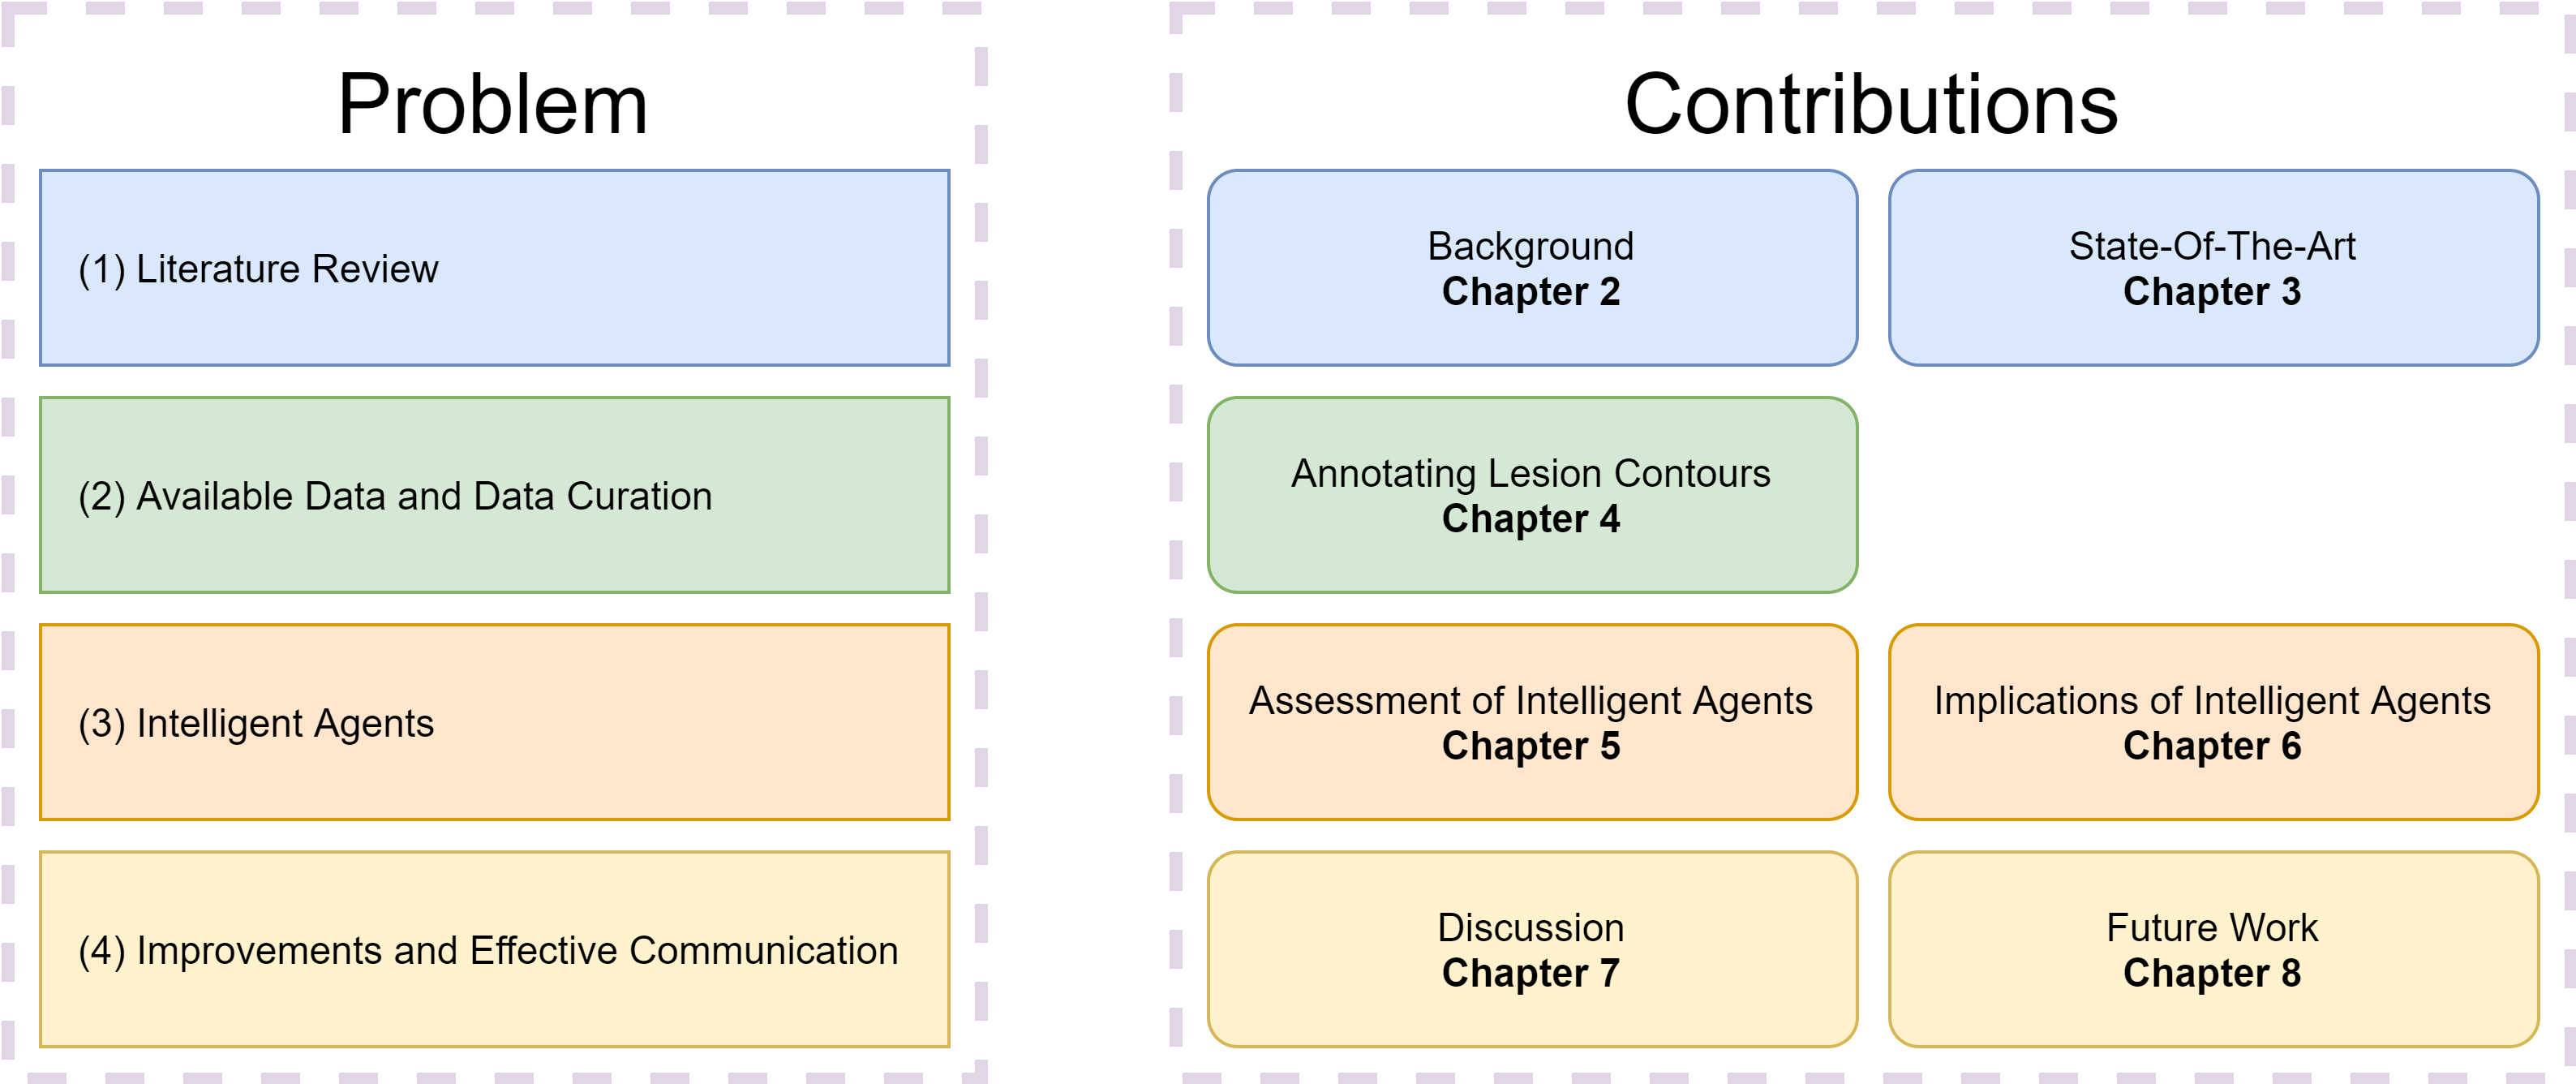
\includegraphics[width=\textwidth]{images/fig017}
\caption{[DOI: \protect\href{https://www.doi.org/10.13140/RG.2.2.14314.95685/1}{10.13140/RG.2.2.14314.95685/1}] Thesis problem and contribution~\cite{https://doi.org/10.13140/rg.2.2.14314.95685/1} relations. In this research, four scientific problems were addressed: (1) mitigating the bias between the clinical background of the medical imaging workflow and the related work of intelligent agents among the research communities; (2) developing a framework for annotating lesion contours to cover the lack of available and curated medical data problem; (3) the problems of assessment and implications of intelligent agents in the medical imaging workflow; and (4) the need for functionality improvements and effective communication of the intelligent agents.}
\label{fig:fig017}
\end{figure}
%%%%%%%%%%%%%%%%%%%%%%%%%%%%%%%%%%%%%%%%%%%%%%%%%%%

Several contributions are solving each problem (Figure~\ref{fig:fig017}) addressed in this thesis.
Although this document focus on the thesis main goals and contributions, one important objective of the document is to provide information concerning the medical imaging background and review of the literature for \ac{HCI} related work.
Thereafter, Chapter~\ref{chap:chap002} and Chapter~\ref{chap:chap003} are aiming to improve the understating of clinicians, researchers, engineers and policy makers in developing robust and effective data-driven interventions across the breast cancer domain.
In problem one, the literature review was stated as a problem and the respective contributions are present in this two chapters.
Moreover, problem four (covered by Chapter~\ref{chap:chap007} and Chapter~\ref{chap:chap008}) discuss and debate the achieved contributions.
In the end, it conclude the clinicians' needs for functionality improvements and effective communication of the intelligent agents, as well as the future work ahead of this thesis.
However, to simplify the central contributions, the next section (Section~\ref{sec:sec001003}) will just list the main contributions to solve problem two (covered by Chapter~\ref{chap:chap004}) and three (covered by Chapter~\ref{chap:chap005} and Chapter~\ref{chap:chap006}), respectively.

This thesis is one of the first contributions to address the above list of problems.
The effort to address each problem to the respective set of contributions, does not rely on any capacity or exercise in futuristic imagination.
Rather, the document aim to clarify the extent in which Humans and \ac{AI} techniques can be put under the evocative rubric of ``\ac{HAII}'' to improve the breast cancer diagnosis.

\clearpage

\section{Contributions}
\label{sec:sec001003}

The main contributions achieved so far are the following:

\begin{enumerate}
\item The design of an advanced visual interface to provide available and curated medical data for the annotation of lesion contours (masses and microcalcifications) on a multimodal strategy of the breast cancer diagnosis; ({\bf Chapter~\ref{chap:chap004}})
\begin{enumerate}[label*=\arabic*.]
\item The visualization of the two main types of breast lesions in \ac{MG}, \ac{US} and \ac{MRI} modalities of medical imaging;
\item Insights from the field comparison of single-modality {\it vs} multi-modality for screenings of breast cancer diagnosis with 31 clinicians and 566 images;
\end{enumerate}
\item Integration of several \ac{AI} techniques, using \acp{DNN}, to support automatic and reliable classification in medical imaging; ({\bf Chapter~\ref{chap:chap005}})
\item Development of a novel \ac{AI} system based on intelligent agents to support a multi-modal imaging strategy; ({\bf Chapter~\ref{chap:chap005}})
\begin{enumerate}[label*=\arabic*.]
\item User study findings of 45 clinicians comprising nine clinical institutions;
\item List of design recommendations for visualization to support breast screening radiomics;
\item Evidence from the impact of multimodality and \ac{AI}-assisted strategy in diagnosing and severity classification of lesions;
\item Evaluation results of a proof-of-concept prototype for the \ac{AI}-assisted condition;
\end{enumerate}
\item Introduction of an \ac{AI}-assisted system in the medical imaging workflow which provides an automated diagnostic based on the developed \ac{DL} methods; ({\bf Chapter~\ref{chap:chap006}})
\begin{enumerate}[label*=\arabic*.]
\item Quantitative and qualitative results to measure:
\begin{enumerate}[label*=\arabic*.]
\item How receptive are the clinicians to the introduction of \ac{AI}-assisted medical imaging and agent-based systems;
\item How they accept and interact with these systems;
\item How \ac{AI}-assistance influence the \ac{UX} perception in the clinical context;
\end{enumerate}
\item Introduction and study for the impact of an intelligent agent into a real-world case study of 45 clinicians from nine institutions;
\item Accuracy comparison (measured in terms of \acp{FP} and \acp{FN} metrics) of \ac{AI}-assisted results;
\item Study the impact of several design techniques on the expectations and satisfaction of the clinicians in different groups of medical professional experience.
\end{enumerate}
\end{enumerate}

\clearpage

\section{Future Objectives}
\label{sec:sec001004}

Several objectives have been accomplished so far, as discussed in the two (Section~\ref{sec:sec001002} and Section~\ref{sec:sec001003}) previous sections.
However, work is still in progress and some goals have not been accomplished yet.
This section provides a direction to the most relevant future milestones, which are addressed in Chapter~\ref{chap:chap008}, as well as some ideas on how to deal with them.

The last part of the thesis main contributions (Chapter~\ref{chap:chap006}) consists in addressing implications for the introduction of intelligent agents as a clinical problem.
This means taking into account that \ac{AI} algorithms are not perfect, as well as what are the clinicians' needs concerning the provided information coming from the agents.
The implications are several and the future objectives must take into account what are the current hazards of each agent to fulfill the respective use case for a better patient diagnostic.
New agent functionalities must be improved to achieve a more effective communication of the agent.
Also, although this document have focused mainly on the development of intelligent agents, there is still room for improvements and further work to be done.

One important issue that the thesis covers is the lesion annotation (Chapter~\ref{chap:chap004}) so that the \ac{AI} algorithms have available and curated data.
On the one hand, the quality of annotation depends on the clinician’s experience.
On the other hand, it also depends on the number of study cases, such as:
(i) annotations made manually by clinicians useful to extract functionalities like lesion contours;
(ii) shape and margins that can be used in the computation of lesion segmentation; and
(iii) classification made by intelligent agents.
In this work, several new functionalities must be integrated~\cite{hugo2020si} to support a higher and better annotation process.
Therefore, the introduction of the following four new functionalities is important:
(1) Recorded View ;
(2) Temporal Comparison View ;
(3) Coordinated View ; and
(4) 3D Module View.
The functionalities aim to lower the annotations time and to improve its precision.

Overstated expectations about \ac{AI}~\cite{https://doi.org/10.13140/rg.2.2.25412.68486, calisto2019midaaiarfuv} and unknown levels of assertiveness decrease user acceptance and adoption of clinical systems.
In particular, when expectations are not met, clinicians' levels of trust will decrease during time~\cite{Kocielnik:2019:YAI:3290605.3300641}.
Another future objective is to study and understand how the level of assertiveness~\cite{10.1145/3311350.3347162, pacheco2019alignment}, will impact the clinicians' decision-making during diagnostic.

In these intelligent agents, most functionalities are seen by clinicians with limited computational knowledge as `black boxes'~\cite{10.1145/3313831.3376807}.
A future objective is enabling clinicians to explore and understand the \ac{AI} results.
In this work, such goal can be achieved by the integration of the \ac{XAI} topic with different setups.
For instance, {\it Agent A} explains the classification results of the patient, while {\it Agent B} explains the segmentation results.
Indeed, they are different \ac{DNN} methods.
The first agent ({\it i.e.}, {\it Agent A}), can be explaining the results coming from \ac{CNN} models ({\it e.g.}, DenseNet~\cite{Huang_2017_CVPR}, ResNet~\cite{He_2016_CVPR}, between others~\cite{10.1117/12.2549103}) as image classifiers.
On the contrary, the second agent ({\it i.e.}, {\it Agent B}), can be explaining the results coming from models ({\it e.g.}, HyperDense-Net~\cite{8515234}, U-Net~\cite{10.1007/978-3-319-24574-4_28} or different ones~\cite{10.1007/978-3-030-46640-4_23}) for image segmentation.

\clearpage

The only intelligent agent described in this document (Chapter~\ref{chap:chap005} and Chapter~\ref{chap:chap006}) use an image classifier ({\it i.e.}, DenseNet~\cite{Huang_2017_CVPR}), that is limited for image classification.
Thus, clinicians cannot understand the decision of such system.
For example, when the system fails, it is difficult to know the reason.
One \ac{DNN} method was integrated with the intelligent agent to classify the cancer severity of each patient, but these medical clues have not yet been used for an automatic lesion segmentation.
Instead, to output the heatmaps (Chapter~\ref{chap:chap005} and Chapter~\ref{chap:chap006}), we are using the manual annotations by computing the circularity of the lesion~\cite{DALILA2017749} and color-related to the computed severity.
However, clinicians do not diagnose patients solely using image information.
As described in Chapter~\ref{chap:chap002}, different patient aspects are considered before performing the final diagnosis.
In order to develop a fully clinically oriented agent it will be necessary to address more methods and other clinical co-variables.

\section{List of Publications}
\label{sec:sec001005}

The work developed in this thesis was published in conference and journal papers. The following sections will list the set of publications published and/or under revision (but accepted) until now.

\subsection{Conference Papers}
\label{sec:sec00100501}

\begin{enumerate}
\item Francisco M. Calisto, Alfredo Ferreira, Jacinto C. Nascimento, and Daniel Gonçalves. 2017. Towards Touch-Based Medical Image Diagnosis Annotation. In Proceedings of the 2017 ACM International Conference on Interactive Surfaces and Spaces (ISS '17). Association for Computing Machinery, New York, NY, USA, 390–395. DOI: \href{https://doi.org/10.1145/3132272.3134111}{https://doi.org/10.1145/3132272.3134111}
\item Francisco Maria Calisto, Nuno Nunes, and Jacinto C. Nascimento. 2020. BreastScreening: On the Use of Multi-Modality in Medical Imaging Diagnosis. In Proceedings of the International Conference on Advanced Visual Interfaces (AVI '20). Association for Computing Machinery, New York, NY, USA, Article 49, 1–5. DOI: \href{https://doi.org/10.1145/3399715.3399744}{https://doi.org/10.1145/3399715.3399744}
\end{enumerate}

\subsection{Journal Papers}
\label{sec:sec00100502}

\begin{enumerate}
\item Francisco Maria Calisto, Carlos Santiago, Nuno Nunes, and Jacinto C. Nascimento. Radiomics Hope or Hype? An HCI Assessment of AI-Assisted Medical Imaging for BreastScreening. International Journal of Human-Computer Studies. [UNDER REVISION]
\end{enumerate}
% If Printing on DOUBLE SIDED pages, the second page should be white.
% Otherwise, comment the following command:
\cleardoublepage
%
% Chapter 2
% #############################################################################
% This is Chapter 2
% !TEX root = main.tex
% #############################################################################
% Change the Name of the Chapter i the following line
\fancychapter{Problem Context}
\clearpage
% The following line allows to ref this chapter
\label{chap:chap002}

Chapter~\ref{chap:chap002} provides valuable background information about the breast cancer domain in the context of this thesis.
While it does not present any original contributions, it can be omitted by readers already familiar with the subject matter~\cite{doi:10.1148/ryai.2020190208}.
For more comprehensive details, including additional background information and medical specifications, please refer to Appendix~\ref{chap:app001}.

\section{Medical Imaging Diagnosis}
\label{sec:chap002001}

\textcolor{revised}{Screening for early detection of breast cancer, while crucial, faces challenges due to the increasing volume of data\footnotemark[4] and the limited throughput capabilities of radiologists~\cite{McKinney2020}.
The processing of this data, essential for timely and reliable diagnosis, is becoming increasingly demanding, leading to a significant workload on clinicians~\cite{HANNA20181709}.
These difficulties have been the driving force behind the recent trend in {\it radiomics} (Section~\ref{sec:chap002006}) and the integration of \ac{AI} techniques into medical imaging~\cite{doi:10.1148/radiol.2015151169}.
For a more detailed exploration of these challenges, please refer to Section~\ref{sec:app001001} in Appendix~\ref{chap:app001}.}

%%%%%%%%%%%%%%%%%%%%%%%%%%%%%%%%%%%%%%%%%%%%%%%%%%%
\footnotetext[4]{Involving the high-throughput extraction of quantitative imaging features, {\it radiomics} intent of creating mining information from radiological images. Large-scale data sharing is necessary for the validation and full potential that {\it radiomics} represents.}
%%%%%%%%%%%%%%%%%%%%%%%%%%%%%%%%%%%%%%%%%%%%%%%%%%%

\section{Breast Cancer Domain}
\label{sec:chap002002}

\textcolor{revised}{During breast cancer diagnosis (Figure~\ref{fig:fig005} on Section~\ref{sec:app001002} of Appendix~\ref{chap:app001}), the use of multi-modal data is critical~\cite{10.1117/1.JBO.22.4.046008}.
\ac{MG}, the primary screening modality, is less effective in dense breasts, posing diagnostic challenges~\cite{10.1093/jbi/wbaa010}, where \ac{US} and \ac{MRI} are used to complement diagnosis~\cite{SHAN2016980}.
However, the variance in diagnostic accuracy across modalities and the demand for combined use significantly increases clinicians' workload, highlighting the need for more efficient and precise diagnostic methods.
This leads to 48\% of radiologists experiencing significant {\it frustration}~\cite{CALISTO2021102607}.
Using \ac{MG}~\cite{10.1001/jamaoncol.2023.4519}, \ac{US}~\cite{doi:10.1200/JGO.19.00127}, and \ac{MRI}~\cite{doi:10.1148/radiol.2021210325} together, elevates the risk of medical errors to as high as 40\% during diagnosis.
Thus, advanced technology integration is vital to enhance diagnostic accuracy and reduce healthcare professional burden.}

\section{Severity Classification}
\label{sec:chap002003}

Clinical guidelines emphasize the importance of regular image screenings for evaluating the risk of breast cancer~\cite{MIAO201817}.
To enhance consistency in the interpretation of imaging findings, the \acs{ACR} introduced the \acs{BI-RADS}~\cite{d2018breast}, which provides a standardized process (Figure~\ref{fig:fig020} on Section~\ref{sec:app001003} of Appendix~\ref{chap:app001}) for describing imaging characteristics and a classification framework with six categories to assess the probability of malignancy.
In the present study, a \acs{DNN} was trained to perform \acs{BI-RADS} classification (Section~\ref{sec:app004003} of Appendix~\ref{chap:app004}).
While this section offers a concise overview of severity classification, Section~\ref{sec:app001003} of Appendix~\ref{chap:app001} delves into further details regarding breast lesion classification.

\section{Lesion Typification}
\label{sec:chap002004}

The lesion typification~\cite{doi:10.1148/radiol.2018181371} is also challenging in this thesis background.
The goal of this section is to explain what is the importance of the lesions, {\it i.e.}, masses (Section~\ref{sec:chap002004001}) and the microcalcifications (Section~\ref{sec:chap002004002}), that will feed the \ac{AI} algorithms (Chapter~\ref{chap:chap005} and Chapter~\ref{chap:chap006}) and provide visual information to clinicians.
For the severity classification~\cite{8611096, 9231684}, it is essential to know the type of mass shapes, microcalcification patterns, and size to understand their importance to the algorithms.
This section summarizes the importance of lesion typification, which will be further detailed in Section~\ref{sec:app001004} of Appendix~\ref{chap:app001}.

\subsection{Masses}
\label{sec:chap002004001}

Mass typification is a crucial aspect of a breast cancer diagnosis.
Benign masses commonly exhibit round, oval, or lobular shapes, while malignant masses are often characterized by lobular, irregular, or architectural distortion shapes (Figure~\ref{fig:fig021} on Section~\ref{sec:app001004001} of Appendix~\ref{chap:app001}).
Margins play a significant role in lesion evaluation.
A circumscribed margin indicates a benign lesion, whereas microlobulated, indistinct, and spiculated margins raise suspicion, with spiculated margins being the most concerning.
An obscured margin, where part of the margin is concealed by fibroglandular tissue, necessitates further investigation, such as an \ac{US} examination (Figure~\ref{fig:fig018}).
It is important to note that this section summarizes the topic, with further details to be presented in Section~\ref{sec:app001004001} of Appendix~\ref{chap:app001}.

\subsection{Microcalcifications}
\label{sec:chap002004002}

In this section, we provide an overview of microcalcification typification, covering five types and their corresponding patterns (Figure~\ref{fig:fig022} on Section~\ref{sec:app001004002} of Appendix~\ref{chap:app001}).
These patterns include diffuse, regional, group, linear, and segmental, each representing distinct characteristics of microcalcifications.
Understanding these patterns is crucial in diagnosing and assessing the severity of breast cancer.
Further details about microcalcification patterns will be discussed in Section~\ref{sec:app001004002} of Appendix~\ref{chap:app001}.
It's important to note that a comprehensive and accurate dataset for clinicians and \ac{AI} algorithms requires a multimodal approach beyond mammography (Figure~\ref{fig:fig018}).
The subsequent section (Section~\ref{sec:chap002005}) will explore the current imaging workflow and emphasize the significance of multi-modal data availability.

\section{Radiology Reading Room}
\label{sec:chap002005}

This section summarizes the intricate radiological workflow, further detailed in Section~\ref{sec:app001005} of Appendix~\ref{chap:app001}.
The radiological workflow consists of three stages:
(1) {\it examination};
(2) {\it diagnosis}; and
(3) {\it report}.
Understanding each stage is vital for both the \ac{HCI} and \ac{AI} communities, as it offers valuable insights into the advancements made in this thesis, particularly in assisting radiologists.

During the {\it examination} (Section~\ref{sec:app001005001}) stage, the radiologist reviews patient records and correlates medical imaging with other relevant information.
The {\it diagnosis} (Section~\ref{sec:app001005002}) stage involves analyzing medical images and utilizing various sources of information to enhance accuracy.
Finally, the {\it report} (Section~\ref{sec:app001005003}) stage captures the radiologist's findings and is a critical communication tool for other healthcare professionals.
In Section~\ref{sec:app001005004} of Appendix~\ref{chap:app001}, we also summarize the main clinical procedures involved in the radiological workflow.

\section{Radiomics}
\label{sec:chap002006}

\ac{DL} has emerged as a powerful asset in {\it radiomics}~\cite{litjens2017survey}, improving the accuracy of breast cancer diagnoses.
These \ac{DL} models are contributing significantly to the {\it radiomics} pipeline (Figure~\ref{fig:fig023} on Section~\ref{sec:app001006} of Appendix~\ref{chap:app001}), including image pre-processing, feature extraction, and classification~\cite{10.1007/978-3-030-59716-0_71}.
However, their `black box' nature, need for extensive annotated data, and data privacy concerns pose challenges~\cite{litjens2017survey}.
This thesis explores these challenges and solutions, emphasizing the role of \ac{HCI} in enhancing trust and adoption of \ac{AI}-assisted medical tools (Chapter~\ref{chap:chap004}).
Further insights into the role of \ac{DL} models in {\it radiomics} are provided in Section~\ref{sec:app001006} of Appendix~\ref{chap:app001}.

\section{Medical Imaging Standards}
\label{sec:chap002007}

This section summarizes the \acs{DICOM} format, a widely used medical standard for storing images~\cite{Trivedi2019}.
It supports various medical information types and file format conversions.
\acs{DICOM} files use associative arrays for hierarchical data structures (Figure~\ref{fig:fig025} on Section~\ref{sec:app001007} of Appendix~\ref{chap:app001}), with each key referred to as a \acs{DICOM} tag.
Standardizing these tags improves readability and facilitates the storage of exams and patient information (Section~\ref{sec:chap002008}).
Further details on this topic can be found in Section~\ref{sec:app001007} of Appendix~\ref{chap:app001}.

\section{Medical Imaging Storage}
\label{sec:chap002008}

The \acs{PACS}~\cite{carter2018digital} offers efficient storage and a simple way to access the \acs{DICOM} images in a variety of modalities.
The deployment of these technologies requires specific packages and environments, which will be further detailed in Section~\ref{sec:app001008} of Appendix~\ref{chap:app001}.
Our platform provides essential tools for deploying multimodality strategies, interactive image visualization/manipulation, and study navigation in a web browser.
This paves the road for integrating multimodality strategies into, \acs{PACS} as it only needs a web browser that is always accessible on clinical workstations.
Further details on deploying these technologies and environments can be found in Section~\ref{sec:app001008} of Appendix~\ref{chap:app001}.
% If Printing on DOUBLE SIDED pages, the second page should be white.
% Otherwise, comment the following command:
\cleardoublepage
%
% Chapter 3
% #############################################################################
% This is Chapter 3
% !TEX root = main.tex
% #############################################################################
% Change the Name of the Chapter i the following line
\fancychapter{State-Of-The-Art}
\clearpage
% The following line allows to ref this chapter
\label{chap:chap003}

In this chapter (Chapter~\ref{chap:chap003}), the document provide an overview on relevant literature works to the content of this thesis.
The document outlines the role of intelligent agents and how other authors are handling their work in various steps of the clinical workflow, including novel interactive systems in medical imaging, application of \ac{HCI} techniques in the domain and \acp{UI} with \ac{AI} methods behind.
To substantiate this thesis, the next sections will summarize important contributions in the particular domain of medical imaging and the role that \ac{HCI} and \ac{AI} topics are playing in this context.

\section{Literature Challenges}
\label{sec:chap003001}

Medical imaging systems allow the end-user to diagnose several modalities, such as \ac{MG}, \ac{US} or \ac{MRI}, from a seamless retrieval medical imaging data~\cite{faraji2019radiologic, seifabadi2019correlation}.
By bringing those modalities together, it offers new possibilities for quantitative imaging ({\it e.g.}, {\it radiomics}) and diagnosis but also requires specialized data handling, post-processing and novel visualization methods~\cite{Igarashi:2016:IVS:2984511.2984537, Ocegueda-Hernandez:2016:CMN:2876456.2879485, Sousa:2017:VVR:3025453.3025566}.
In the clinical domain, medical imaging tools can help experts make better decisions~\cite{Lopes:2017:UHC:3143820.3144118}, {\it e.g.}, by identifying cancer prognostics among the available multi-modal data~\cite{lopes2018interaction}.

A wide range of new contributions for medical imaging systems exist, providing clinicians with the knowledge to enhance the clinical workflow~\cite{Cai:2019:HTC:3290605.3300234, edge2019clinical}.
From systems that supply potential information~\cite{10.1145/3399715.3399744, 10.1145/3206505.3206555}, to decision-making systems~\cite{10.1145/3290605.3300468, 10.1145/3359206}, these new contributions are improving the diagnostic decisions of medical professionals~\cite{hwang2019artificial}.
Although several studies have shown that \ac{AI} systems can reduce medical error and improve outcomes~\cite{Cai:2019:HTC:3290605.3300234, Cai:2019:EEE:3301275.3302289}, one traditional difficulty is the lack of user trust and acceptance~\cite{https://doi.org/10.1002/mp.13562}.
On the one hand, experts may resist using a system if it does not capture the nuances of their mental models or provides relevant context~\cite{khairat2018reasons, kohli2018cad, yang2016investigating}.
On the other hand, clinicians are known to resist changes and new tools~\cite{10.1145/3132272.3134111, gagnon2014electronic}, an issue that has an impact in their workflow.

Despite the breakthroughs and progress in the context of \ac{AI} in medical imaging, one challenge regarding \ac{DL} approaches is its `black box' characteristics~\cite{10.1007/978-3-030-50334-5_4, 10.1145/3306618.3314293}.
Due to the high degree of complexity of \ac{DL}-based approaches such as \acp{NN}, there is no inherently comprehension understanding of the internal processes~\cite{8851763}.
\ac{AI} systems that suffer from this problem are often referred to as opaque~\cite{zednik2019solving}.
Hence, there is the trade-off between performance and explainability: while performance of models increase, the explainability of these approaches decrease~\cite{gunning2017explainable}.
In order to achieve higher transparency, new techniques to improve the interaction of humans and \ac{AI} must be addressed.

In this section, the document focus on understanding different aspects and challenges that other authors surpassed for the integration of their systems into the medical workflow.
In particular, their work demonstrates how an interactive system can directly address the above mentioned issues during medical imaging diagnosis.
The next section, introduce the topic of \ac{HAII}, as well as several related works, explaining the importance of the topic to this thesis work.

\section{Human-AI Interaction}
\label{sec:chap003002}

Applications of \ac{HAII} collaboration~\cite{dellermann2019future} in complex domains are subject to the following two issues:
(1) trust, transparency and accountability of the involved \ac{AI} agent~\cite{10.1145/3290605.3300233}; and
(2) user's ability to understand and predict agent behavior, {\it i.e.}, explainability and intelligibility~\cite{Cai:2019:EEE:3301275.3302289, gunning2017explainable, miller2018explanation}.
Forming accurate mental models of the \ac{AI}-assisted is useful for:
(i) representing the clinician's belief about what the system can do, acquired via interviews and observations, instruction, or inference;
(ii) mapping between the observable features of the developed framework and the functionality perceived by the user; and
(iii) the prediction for anticipating the \ac{AI} output in a given scenario.

In that context, several studies in user expectations~\cite{Kocielnik:2019:YAI:3290605.3300641, leung2019health} are postulating that user satisfaction and acceptance of a system is directly related to the difference between initial expectations and their actual experience.
Specifically, expecting more than the system can deliver will decrease user satisfaction and lead to the rejection of the system.
Hence, in the proposed work of this thesis a technique was created, based on the following contributions:
(a) providing users a new control feature on the introduction of \ac{AI} methods among medical imaging diagnosis~\cite{pesapane2018artificial}; and
(b) the impact of the clinicians' {\it behaviour}, as well as the impact in professional practice~\cite{Challen231}.
In the end, the final goal was to achieve more reliable expectations of each intelligent agent capabilities, addressing these potential gaps.

The growing prevalence of \ac{DL} models and their use in decision-making have led to increasing demands for more transparent and explainable results~\cite{10.5555/3305381.3305576}.
However, the interpretation of \ac{DL} models is challenging due to their complexity and often opaque internal state.
Thus, the \ac{ML} community has produced a myriad of algorithmic methods to explain their inner working~\cite{Shakerin_Gupta_2019, 10.1145/3329859.3329878}.
These methods aim to explain the model prediction outcome with two main reasons:
(1) for a single input data point~\cite{10.1145/2939672.2939778}; and
(2) for a set of data points in a predicted class~\cite{pmlr-v80-kim18d}, often by perturbing the inputs of the model and watching how the model response to changes.
Across this work, there is a clear need to ensure usability and efficacy with real users~\cite{10.1145/3173574.3174156}.
Consequently, a recent hype in \ac{HCI} research has studied what the end-user actually desire to understand the \ac{ML} results, as well as how that transparency affects user attitudes and behaviour.
Hence, the final outcomes are also (hopefully) improved which answers to what questions the user may desire to ask the \ac{AI} system.

Recent works on accountability and fairness have proposed the use of short records with trained \ac{ML} models revealing their intended use, details of their performance evaluation of procedures, and the potential biases that they may embody~\cite{10.1145/3351095.3375709, 10.1145/3287560.3287596}.
Additionally, others have studied whether people's trust varies depending on the stated accuracy of the model and how it differs from observed accuracy in practice~\cite{10.1145/3290605.3300509}.
In this thesis, the document builds on a growing interest in studying the broader, global aspects of model transparency, and conducts a deep exploration of these issues within the domain of decision-making in medical imaging.
The following section will discuss recent advances on the introduction of \acp{CDSSe} in the medical workflow.

\section{Clinical Decision Support}
\label{sec:chap003003}

Most of the best performing \acp{CDSSe}\footnotemark[8] rely on \ac{ML} algorithms that learn specific tasks from training data.
The field recently gained enormous interest, mostly due to the practical successes of \ac{DL}~\cite{meacham2019towards}.
The rapid and widespread development of \ac{DL} methods supports a wide range of image analysis tasks, including classification, detection, and segmentation \cite{lecun2015deep}.

%%%%%%%%%%%%%%%%%%%%%%%%%%%%%%%%%%%%%%%%%%%%%%%%%%%
\footnotetext[8]{The term was designated for computer applications that are designed to aid clinicians in making diagnostic and therapeutic decisions for patient care. In this thesis, we use this definition to define it as active knowledge systems for clinical advice.}
%%%%%%%%%%%%%%%%%%%%%%%%%%%%%%%%%%%%%%%%%%%%%%%%%%%

\ac{DL} methods rely on large annotated datasets to learn essential and to discriminate image features for each specific task, with performances matching and even surpassing humans~\cite{esteva2017dermatologist, McKinney2020}.
In medical applications, \ac{DL} has also been the major contributor to the success of \acp{CDSSe}~\cite{esteva2019guide}, {\it e.g.}, on the diagnosis of skin cancer \cite{esteva2017dermatologist}, the segmentation of cardiac \ac{MRI}~\cite{medley2019segmenting}, or breast cancer detection~\cite{MAICAS2019101562}.
Their outstanding performance in identifying meaningful patterns within the available data was recently used to help humans learn new biomarkers of specific diseases \cite{cole2017predicting, gonzalez2018deep, wang2019deep}, suggesting these models can see beyond what a trained radiologist sees in medical images.

Despite their success, these systems are becoming increasingly more complex and incomprehensible to the users~\cite{holzinger2019causability}.
This gave rise to a critical challenge, particularly for medical applications, where results provided by an \ac{AI}-assistance does not explain the decision of the model~\cite{shah2019artificial}.
Two approaches are currently proposed to address this challenge: \ac{XAI} and Intelligibility~\cite{gunning2017explainable, miller2018explanation}.
\ac{XAI} and Intelligibility, in the clinical context, must take into account that diverse data may contribute to a relevant result~\cite{Bharadhwaj:2019:ERS:3308557.3308699}.
The work done by Holzinger et al.~\cite{holzinger2018current} addresses this need, underlining that clinicians must have the possibility to understand {\it how} and {\it why} a machine decision was reached.
Moreover, transparent algorithms could appropriately enhance the trust of clinicians in future Human-AI interactions~\cite{Dominguez:2019:EEA:3301275.3302274, Weisz:2019:BTS:3301275.3302290}.

The work developed by Cai et al.~\cite{Cai:2019:HTC:3290605.3300234} identify the needs of clinicians when searching for similar images using a \ac{DL} algorithm.
The developments that empower users through this task, are informing the thesis work concerning the communication of what types of similarity are most important at different moments in time.
Their work demonstrate how a \ac{CDSSe} can directly address the issues of user acceptance and trust during medical image search.

In another work, Cai et al.~\cite{10.1145/3359206} findings reveal that, far beyond understanding the local, case-specific reasoning behind any \ac{AI} model decision, clinicians desired upfront information about basic, global properties of the model.
Here, clinicians preferences are based in the model {\it known strengths} and {\it limitations}.
Moreover, their findings show to this thesis work that clinicians want to know the model subjective {\it point-of-view}, and its overall {\it design} objective, so that clinicians can understand what is the model designed to be optimized for.
In short, their findings broaden and enrich discussions surrounding \ac{AI} transparency for decision-making, providing to this thesis a richer understanding of what experts find important in their introduction to intelligent agents before integrating them into routine practice.

Finally, the work investigated by Yang et al.~\cite{10.1145/3290605.3300468} describes the design and field evaluation of a radically new \ac{CDSSe}.
In this work, the authors developed a system which automatically generates information for clinicians' decision-making with subtly embedded machine prognostics.
Their design took inspiration from the notion of Unremarkable Computing~\cite{Crabtree2020}, that by augmenting the clinicians' workflow can have significant importance for yet remain unobtrusive.
The work evaluation suggests clinicians are more likely to encounter and embrace such a \ac{CDSSe}.
In the end, the authors discuss the importance and intricacies of finding the right level in the \ac{CDSSe} design, sharing lessons learned so important to this thesis work in prototyping critical \ac{AI} systems as a situated experience.

However, the works addressed in this section do not inspect the problem that medical assessments can be contentious, leading to expert disagreement.
This raises the question of how assistive technologies and \ac{AI} systems should be designed to handle a better diagnostic of ambiguous \ac{AI} results.
In the following sections, the document will explain how some studies are covering the problem of diagnosing such ambiguity by the design of assistive technologies while informing clinical uncertainty estimates.

\section{Medical Image Assessment}
\label{sec:chap003004}

A strong need for large amounts of annotated medical data has been created by the rise of \ac{DL} methods and \ac{AI}-assisted medical decision-making tools~\cite{10.1145/3313831.3376290}.
In most cases, the ground-truth annotations required to develop supervised \ac{ML} algorithms ({\it e.g.}, diagnostic corrections) are not given in the raw data.
These settings require the expertise from medical professionals for manual data annotations.

Like any form of human interpretation, medical data analysis by clinical experts is a subjective process and can lead to conflicting medical image assessments among independent clinicians~\cite{NIAZI2019e253, granzier2020mri, DEMCHIG201962}.
The issues of inter-variability and intra-variability disagreement\footnotemark[9] are particularly critical within medicine where unreliable clinical decisions can impact patients' lives adversely.
Hence, classification and segmentation disagreement poses a full-fledged clinical problem in the medical imaging domain~\cite{TANNO2021117366, raghu2019direct}.

Prior work in \ac{HCI} for medical relation extraction~\cite{10.1145/3152889} substantiate the disagreement relations between inter-variability and intra-variability.
In this thesis, the disagreement relations are addressed as a function of three phenomena: (1) differences among clinical professionals, such as the medical background of each clinical institution and bias; (2) heterogeneous characteristics of the dataset to be analysed, such as noisy and heterogeneous modalities; and (3) the quality of the diagnostic guidelines, such as the subjective and ambiguous classification of the \ac{BI-RADS}.
In fact, clinical experts often rely on complex viewing technology to inspect medical data.
Making it vital to find additional sources.

%%%%%%%%%%%%%%%%%%%%%%%%%%%%%%%%%%%%%%%%%%%%%%%%%%%
\footnotetext[9]{In order to express variability relations, this document report two measures of the \ac{CV} as: (a) inter-variability; and (b) intra-variability. The \ac{CV} is a measure that is defined as the \ac{SD} for a set of measurements divided by the mean of that same set. In this thesis, it was considered the inter-variability (\ac{CV}\textsubscript{inter}) as the \ac{CV} results of all clinicians' set while diagnosing each patient. On the other hand, intra-variability (\ac{CV}\textsubscript{intra}) represents the \ac{CV} results per (intra) group of medical background.}
%%%%%%%%%%%%%%%%%%%%%%%%%%%%%%%%%%%%%%%%%%%%%%%%%%%

Discrepancies in viewer settings ({\it e.g.}, pan, zoom-in, zoom-out or brightness)~\cite{10.1145/3359178} and sequential dependencies~\cite{schaekermann2018expert} were found to be additional sources of variability for assessments in medical image analysis.
However, the work developed by Schaekermann et al.~\cite{10.1145/3313831.3376290} fulfils these concerns.
In that work, the authors presented the results of clinical professionals with either individual performance alone (intra-variability), or a group of specialists (inter-variability).
From here, this thesis is following the authors' suggestions that image adjudication may provide benefits beyond developing trusted consensus with \ac{AI}, and that exposure can be an effective intervention for medical imaging diagnosis.

\section{Structured Adjudication}
\label{sec:chap003005}

As previously stated, this section address several literature works which are studying the problem of expert disagreement to ambiguous \ac{AI} results for solving divergent medical imaging assessments.
Specifically, expert disagreement is pervasive in clinical decision-making, while medical adjudication is a useful approach for divergent assessments~\cite{10.1145/3359178, SchaekermannMike2020}.
Moreover, prior work~\cite{Aroyo_Welty_2014} shows that expert disagreement can arise due to diverse factors including expert background, the quality and presentation of data, and guidelines clarity.

In the work developed by Schaekermann et al.~\cite{10.1145/3359178}, the authors studied how these factors predict initial discrepancies in the context of medical time series analysis, examining why certain disagreement persist after adjudication.
Also, the authors studied how adjudication impacts clinical decisions which is so important to this thesis work.
Having this idea in mind, Schaekermann et al.~\cite{10.1145/3359178} findings are suggesting that structured adjudication can lead to significant revisions in treatment-relevant clinical parameters such as the generated annotations.
Their work demonstrates how structured adjudication can support consensus and facilitate a deep understanding of experts during medical data analysis.

The process of breast severity classification (Section~\ref{sec:chap002003}) and lesion typification (Section~\ref{sec:chap002004}) involves examination and adjudication~\cite{DODGION2017196} of several modalities ({\it e.g.}, \ac{MG}, \ac{US} and \ac{MRI}), as well as the assessment of several features (Section~\ref{sec:chap002006}).
Such features can be, for instance, extracting texture, shape, and margin (Section~\ref{sec:chap002004001}).
In a medical setting for remote screening~\cite{10.1200EDBK200141}, experts examine breast images to determine the presence and severity of the disease.

Prior work~\cite{MIRANDA2015334} has shown that the process of medical interpretation is subject to individual expert bias, as demonstrated (Chapter~\ref{chap:chap006}) by inter-variability in relation to intra-variability~\cite{NIAZI2019e253}.
This poor agreement between medical experts has led to difficulties in reliable evaluation of both individual experts, as well as assistive technologies.
Yet, due to the lack of medical professionals threatens the adequacy and availability of clinical services, there continues to be a surge in interest for the development of assistive technologies.
These assistive technologies, such as \ac{DL} systems and intelligent agents, are resulting in the sharp increase within the demand for high-quality of annotated-image data.

In another work~\cite{10.1167/tvst.8.6.40}, the authors present and evaluate a remote tool, image-based system, as well as structured classification and annotation for medical imaging adjudication.
Their results show that a remote, tool-based adjudication, can help organize the data generation process (Chapter~\ref{chap:chap004}) and to further disambiguate (Section~\ref{sec:chap003006}) the \ac{AI} results (Chapter~\ref{chap:chap005} and Chapter~\ref{chap:chap006}) of this thesis.
Specifically, for those cases that can be solved with less doubts.
However, their solution falls short for hard cases.
Leading also space to explore new methods that can accelerate the resolution for such hard cases.

\section{Disambiguate Artificial Intelligence}
\label{sec:chap003006}

Among clinical experts, medical discussion can be useful to capture sources of disagreement in ambiguous classification and segmentation of hard cases, as well as adjudicate any resolvable disagreement~\cite{10.1145/3308560.3317085}.
In supervised \ac{ML}, a common requirement is that objects can be unambiguously classified into categories~\cite{castro2020causality}.
However, there are many classification tasks that are inherently ambiguous.
Over the correct way to classify an object, the reasons why clinical experts may be in disagreement with the \ac{AI} results may vary from task to task and from data object to data object.
In this section, the thesis address several researchers who have recognized this problem and come up with different solutions to handle it~\cite{10.1145/3313831.3376506, 10.1145/3313831.3376590, Tschandl2020}.
Between these addressed works, one main distinction can be made around the question of whether expert disagreement with the \ac{AI} results is a problem to be solved or whether disagreements are treated as a signal that leverage in some useful way.

The work developed by Schaekermann et al.~\cite{10.1145/3308560.3317085} is situated along the later line of research.
In that work, the authors propose a key component to trusted and \ac{XAI} systems used to capture and understand the logic arguments, as well as the various pieces of evidence that lead to divergent interpretations.
Their goal is to get one step closer to endowing \ac{AI} systems with the ability of providing argument-based explanations about potentially ambiguous classification during clinicians' decision-making.
Thus, their work was extended to the work developed under this thesis so that it is possible to follow their approach for capturing clinicians' rationale for decision-making in a structured and guided manner.

Other works have suggested ways to make productive use of disagreement information in medical data~\cite{10.1001/jamanetworkopen.2019.0096, 10.1007/978-3-319-11915-1_31, pmlr-v97-raghu19a, 10.1145/3313831.3376506}.
In the work developed by Inel et al.~\cite{10.1007/978-3-319-11915-1_31}, the authors introduced several domain-independent quality measures, task instructions and data, based on information disagreement in medical relation extraction.
Raghu et al.~\cite{pmlr-v97-raghu19a} developed \ac{AI} models to predict the likelihood that a given patient case will cause expert disagreement.
Similarly, Barnett et al.~\cite{10.1001/jamanetworkopen.2019.0096} evaluated different ways of aggregating discordant medical assessments from clinicians with varying training background to harness collective intelligence for medical diagnosis.
Finally, Schaekermann et al.~\cite{10.1145/3313831.3376506, SchaekermannMike2020} studied the conflicting expert assessments that can motivate detailed adjudication discussions about hard cases, and test whether such discussions can improve training for medical experts at a scale.

In conclusion, ambiguous \ac{AI} results are a challenge to be surpassed and must be addressed in this document.
However, to close the gap between \ac{AI} algorithms and clinician's needs for effective transparency, the \ac{HCI} community has called for interdisciplinary collaboration~\cite{10.1145/3173574.3174156, Tschandl2020} and user-centered approaches to explainability~\cite{10.1145/3290605.3300831, 10.1145/3313831.3376590}.
In this section, not only the goal is to address the literature solutions to disambiguate \ac{AI} methods, but also the opportunities and insights into the design of transparent and explainable (\ac{XAI}) techniques for \ac{AI} systems.
Although the audience of this thesis is focused on the \ac{HCI} community, the document must address \ac{DL} and data science literature to fully cover the thesis contributions.
The next sections will cover these concerns.

\section{Deep Learning Methods}
\label{sec:chap003007}

Medical images are hard to classify and segment, because of their anatomical structures (Section~\ref{sec:chap002004}) vary in shape and size~\cite{10.1007/978-3-030-00934-2_99}.
The representational power and capacity for capturing structural information of \acp{CNN}, have made such segmentation (Section~\ref{sec:chap003007001}) and classification (Section~\ref{sec:chap003007002}) possible~\cite{Hou_2016_CVPR, 10.1007/978-3-319-24574-4_28}.
The literature shows that the detection of lesions in breast cancer is highly inconsistent~\cite{shen2019deep, s20143903}.
Breast cancer detection methods can be divided into five~\cite{s20143903} main approaches:
(i) traditional image acquisition techniques;
(ii) image enhancement model, especially for noise removal;
(iii) finding cancer affected areas by detecting the suspicious \ac{ROI} on medical images while using suitable segmentation method;
(iv) feature extraction, such as {\it radiomics}; and
(v) classification of normal, benign or malign from \ac{ROI}.
Making it vital to create a proper model pipeline (Figure~\ref{fig:fig027}) to achieve a better segmentation, feature extraction and classification.

%%%%%%%%%%%%%%%%%%%%%%%%%%%%%%%%%%%%%%%%%%%%%%%%%%%
\begin{figure}[htbp]
\centering
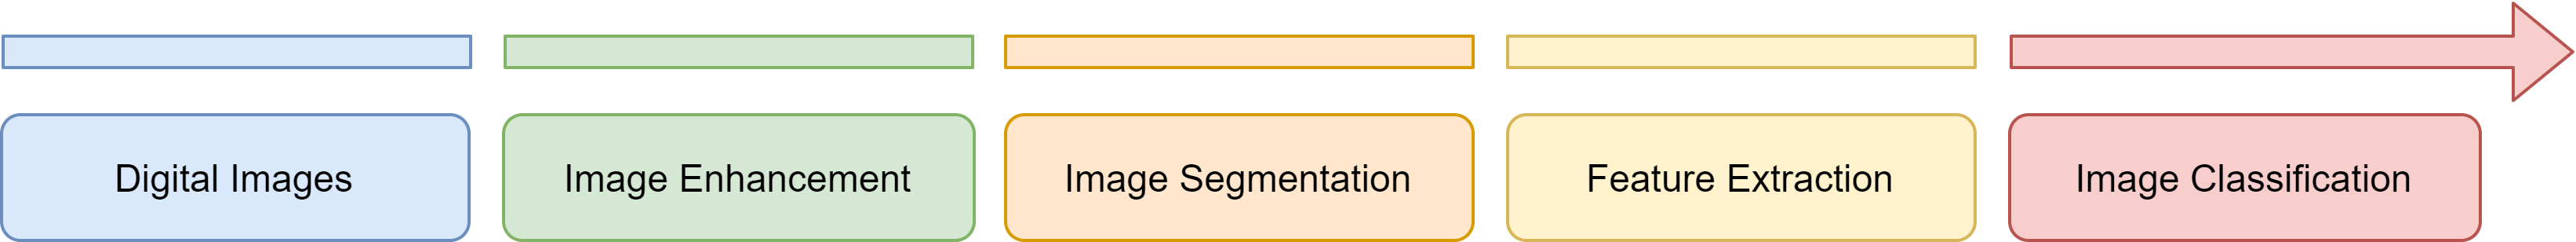
\includegraphics[width=\columnwidth]{images/fig027}
\caption{A simple diagram~\cite{s20143903} for the proposed model pipeline of breast cancer detection. First of all, digital images are acquired. Second, image enhancement must be proceeded. Third, computing image segmentation. Fourth, extraction of features. Fifth and final, classification of images.}
\label{fig:fig027}
\end{figure}
%%%%%%%%%%%%%%%%%%%%%%%%%%%%%%%%%%%%%%%%%%%%%%%%%%%

Several works~\cite{ammar2015semantically, wang2018support, milosevic2017comparison} are addressing many methods for the early detection of breast cancer lesions.
The following sections address each work that is already implemented, or will be implemented, in the work developed under this thesis.
A model for the classification problem was already combined with an intelligent agent and was evaluated (Chapter~\ref{chap:chap005} and Chapter~\ref{chap:chap006}) by clinicians according to early developments of the thesis.
However, the integration of a segmentation model into an intelligent agent is still in progress.
In this work, a classifier was first integrated (Chapter~\ref{chap:chap005}) as a result of clinicians' priority for information concerning the \ac{BI-RADS} classification.
Thus, the segmentation problem is not yet integrated here and will be further addressed (Chapter~\ref{chap:chap008}) as future work.

Although several works~\cite{sharma2020model, 9247957} are arguing to follow a specific pipeline (Figure~\ref{fig:fig027}), it is not mandatory for staying strict to that order, like other authors did~\cite{8451510, AGRAWAL201927}.
During the development and integration of these methods, the order of each process can be changed without loosing model accuracy~\cite{8462671}.
In fact, this thesis is focused on the introduction of intelligent agents as an \ac{HCI} perspective, instead on optimizing the model accuracy.
Therefore, jumping to the final stage of the pipeline (Figure~\ref{fig:fig027}), and start from the end, will be fair to cover the thesis main concerns.

Regarding the above pipeline order ({\it i.e.}, segmentation, feature extraction and classification), each process can be fulfilled separately~\cite{8451510, AGRAWAL201927} and brought together~\cite{10.1007/978-3-030-00934-2_99} in the end of the thesis.
For a proper patient diagnostic, the final classification is actually the most important task~\cite{BHARDWAJ20154611}.
Specifically, the use case achieved from an automatic classification (\ac{BI-RADS}) is the process in which clinicians~\cite{goldenberg2011computer} are informed of the final diagnostic results.
That said, a use case for patient's classification is of a chief importance for the clinicians' workflow~\cite{10.1117/12.2081576}.

In this thesis, the segmentation will support the process of making an intelligent agent more explainable (\ac{XAI}) and interpretable~\cite{8622433}.
For instance, the segmentation can inform the clinician where the lesions are and why ({\it e.g.}, with colours and heatmaps) is the \ac{BI-RADS} so high.
However, segmentation models are more challenging to train~\cite{hesamian2019deep}.
Due to a lack of the available data~\cite{ahmed2020images}, segmentation models are hard to accurately implement in comparison to classification models for the medical imaging domain~\cite{murtaza2019deep}.
One important fact is that image-level labels (weak annotations)~\cite{10.1145/3373017.3373051}, cumming from the classification process, are easier to get for the training set~\cite{TAJBAKHSH2020101693}.
To train a model, the segmentation process is more time-consuming and manual lesion annotations are harder to get from clinicians~\cite{10.1007/978-3-030-59719-1_44}.
Hence, the work under this thesis started first by developing intelligent agents to inform clinicians about the patient classification.

\subsection{Segmentation}
\label{sec:chap003007001}

The above section described several literature works and challenges that this thesis must address to integrate classification and segmentation models into intelligent agents for a proper medical imaging diagnosis.
In this section, the document focus on the works~\cite{7412749, Dabbous397} that will promote and motivate the future integration of segmentation models.
Specifically, one motivation to that integration will be to provide clinicians the visualization of lesions, making these models infer their decisions~\cite{CHOUGRAD201819, doi:10.1148/radiol.2018181371}.
Additionally, the use of these detected lesions can be further applied to aid the training of \acp{DNN}~\cite{8032490, 8861376}.
In this thesis, a multimodality HyperDenseNet~\cite{8515234} model is proposed to be integrated and to solve the segmentation problem.
The task will be to segment inputs of breast images into binary lesion masks, such as masses and microcalcifications.
However, these are just future thoughts being out of the scope of this document, which is describing the work achieved until now.
Therefore, the next section will address important literature for what was done until now under this thesis.

\subsection{Classification}
\label{sec:chap003007002}

From the literature, recent proposed \ac{DenseNet}~\cite{Huang_2017_CVPR} is one of the most used \ac{CNN} structures for the classification of lesions in medical imaging~\cite{LIU2019e271}.
The model connects all the preceding layers as the input for certain layer, which can strengthen feature propagation ({\it e.g.}, {\it radiomics}) and alleviate the gradient vanishing problem~\cite{10.1145/3136755.3143016}.
Furthermore, due to the feature reuse, the \ac{DenseNet} model only needs to learn a small set of new features in each layer.
Thus, the model requires fewer parameters than traditional \acp{CNN}, which is more suitable for small datasets, such as the one created under this thesis.
In this thesis work, a multimodality \ac{DenseNet} model was integrated to solve the classification problem.
The task is to classify inputs of \ac{MG} (both in \ac{CC} and \ac{MLO}), \ac{US}, and \ac{MRI} images.
Along with ground-truth of masses and microcalcifications, the masks of the model can classify (either normal, benign, or malign) into the correct class.

\section{Published Datasets}
\label{sec:chap003008}

In breast screening, published research results are difficult to replicate due to the lack of datasets in the area of \acp{CDSSe}~\cite{lee2017curated}.
Most of the used segmentation (Section~\ref{sec:chap003007001}) and classification (Section~\ref{sec:chap003007002}) methods are evaluated on private datasets~\cite{SADAF2011457} or on unspecified subsets of public databases~\cite{https://doi.org/10.1118/1.4921612}.
These methods are integrated as algorithms for a proper \ac{CADe} and \ac{CADx} on breast cancer and are designed to assist clinicians for a better diagnostic interpretation.
Despite promising results, current \ac{CADe} systems are limited by high \ac{FP} rates~\cite{NISHIKAWA20141320}, and \ac{CADx} systems for breast screening are not yet approved for clinical use because of the lack of available data~\cite{10.1145/3079765}.

Few well-curated public datasets and databases have been provided for breast screening community.
These include INbreast~\cite{MOREIRA2012236}, \ac{MIAS}~\cite{7813261} and \ac{DDSM}~\cite{shen2019deep}.
Although these public datasets are useful, they are limited in terms of data accessibility, completeness and size.
Moreover, datasets are limited in terms of single-modality images ({\it i.e.}, on \ac{MG}-only information) and do not provide any co-variables\footnotemark[10] of the patients.
Such information, is so important to clinicians' workflow.
Furthermore, most researchers are using these datasets without leveraging its images for a variety of reasons~\cite{lee2017curated}.
For instance, the \ac{ROI} annotations for the abnormalities in \ac{DDSM} were provided to indicate a general position of lesions, but not a precise segmentation and classification for them.
Therefore, in this thesis it was also developed a tool (Chapter~\ref{chap:chap004}) that is generating a novel dataset jointly with clinicians.
This feature is covering the implementation problem and limitations of algorithms for accurate feature extraction.

%%%%%%%%%%%%%%%%%%%%%%%%%%%%%%%%%%%%%%%%%%%%%%%%%%%
\footnotetext[10]{The hazard of patient diagnosis must be modelled as a function of several co-variables, such as pathological results, age, morbidity, patient behaviours ({\it e.g.}, smoking), tumour history, between others. Current datasets do not contain any information about these co-variables. A prognostic model that predicts the final diagnostic result and aids in primary clinicians' decision-making must have into consideration these co-variables for early breast cancer detection.}
%%%%%%%%%%%%%%%%%%%%%%%%%%%%%%%%%%%%%%%%%%%%%%%%%%%
% If Printing on DOUBLE SIDED pages, the second page should be white.
% Otherwise, comment the following command:
\cleardoublepage
%
% Chapter 4
% #############################################################################
% This is Chapter 4
% !TEX root = main.tex
% #############################################################################
% Change the Name of the Chapter i the following line
\fancychapter{Acceptance \& Adoption}
\clearpage
% The following line allows to ref this chapter
\label{chap:chap004}

\vspace{0.5mm}

\noindent
{\it Chapter~\ref{chap:chap004} was published in a journal with a Q1 ranking for 2022:}

\vspace{0.5mm}

\begin{itemize}
\item {\bf Francisco Maria Calisto}, Nuno Nunes, Jacinto C. Nascimento, Modeling Adoption of Intelligent Agents in Medical Imaging, International Journal of Human-Computer Studies, Volume 168, 2022, 102922, ISSN 1071-5819, DOI: \href{https://doi.org/10.1016/j.ijhcs.2022.102922}{doi.org/10.1016/j.ijhcs.2022.102922}
\end{itemize}

This chapter investigates the receptiveness of clinicians to intelligent agents in medical imaging.
The aim is to comprehend the determinants of acceptance and adoption of these systems.
We followed the fundamental concepts of the \ac{UTAUT} model, implementing our own and providing insights to enhance the design and integration of intelligent agents into healthcare settings.

\section{Motivation}
\label{sec:chap004001}

In the rapidly advancing field of \ac{AI} research, the medical sector holds significant innovation potential.
\ac{DL} methods have emerged as powerful tools in the clinical domain, enabling a range of advancements such as genome interpretation~\cite{sundaram2018predicting}, medical coaching~\cite{CALISTO2022102285}, assistive scan readings~\cite{madani2018deep}, cancer diagnosis and identification of mutations~\cite{Sollini2020}, and mortality prediction~\cite{ahmad2018death}.
These \ac{AI}-based systems can support clinicians and improve patient care, particularly in cases where radiologic expertise may be limited~\cite{doi:10.1148/radiol.2020201874, doi:10.1148/radiol.2020190283}.
However, to ensure successful implementation and adoption of \ac{AI} systems in real-world clinical settings~\cite{Kocielnik:2019:YAI:3290605.3300641}, it is crucial to address issues of inconsistency and imperfection that can erode clinician trust and lead to technology abandonment~\cite{CALISTO2021102607, CALISTO2022102285}.

Clinicians' trust in \ac{AI} technologies is pivotal for acceptance and usage~\cite{CALISTO2021102607}.
It is vital to understand factors influencing their \ac{AI} adoption to design trustworthy solutions~\cite{JUNGMANN2021834}.
Addressing reliability, consistency, clinical expertise alignment, and privacy, while considering moderator variables, can enhance decision-making processes and patient care.

In this chapter, we investigate the adoption and use of intelligent agents that support clinicians during patient diagnosis via medical imaging.
We aim to understand the factors that influence the acceptance and adoption of these \ac{AI} systems, focusing on risk, privacy, trust, and moderator variables such as gender, age, medical experience, training levels, and areas of expertise~\cite{CALISTO2021102607, Kocielnik:2019:YAI:3290605.3300641}.
Exploring these factors provides valuable insights into clinicians' adoption patterns and enables the enhancement of the design and integration of intelligent agents in healthcare settings.

Despite significant progress in intelligent agents, their widespread acceptance in the clinical field is not assured~\cite{Kocielnik:2019:YAI:3290605.3300641}.
It is crucial to delve into pivotal factors shaping clinicians' behavior towards these agents~\cite{DEANGELI2020102412}.
Unearthing these factors can expedite the integration of these agents, propelling the introduction of \ac{AI} systems in healthcare.
Notwithstanding the promise held by intelligent agents, their actual use by clinicians remains limited compared to their capabilities~\cite{doi:10.1148/radiol.2020201874, doi:10.1148/radiol.2020190283}, highlighting the necessity for ongoing research into their acceptance and adoption.

To provide a theoretical framework for our research, we adopt the \ac{UTAUT} model~\cite{CALISTO2022102922, info:doi/10.2196/27122}.
The \ac{UTAUT} model has successfully explained technology acceptance in various contexts~\cite{DEANGELI2020102412}.
Moreover, its application in the healthcare domain can expand our understanding of the introduction of \ac{AI} in specific healthcare domains~\cite{info:doi/10.2196/27122}.
We aim to analyze clinicians' intentions to use \ac{AI} systems using the \ac{UTAUT} model and enhance its explanatory power and predictive accuracy~\cite{DEANGELI2020102412}.

In this work, we examine clinicians' perceptions and attitudes toward \ac{AI} applications in the medical imaging workflow.
The research objectives are threefold:
(1) to investigate the effects of intelligent agents on technology adoption, with a focus on security, risk, and trust;
(2) to better understand the determinants of trust and acceptance in technology use; and
(3) to improve the explanatory power of a questionnaire based on \ac{UTAUT} constructs for broader application in \ac{HCI} and \ac{AI} research communities.
We employ the \ac{UTAUT} model to analyze clinicians' intention to use an \ac{AI} system~\cite{DEANGELI2020102412}, with the novelty of building a sustainable model tailored to the medical imaging workflow.

Paired with this chapter, Appendix~\ref{chap:app002} provides a more in-depth analysis of our contributions and results.
Section~\ref{chap:app002001} provides a more detailed view of the problem statement, highlighting the research gaps and motivations for our study.
We also outline here the proposed research model (Section~\ref{chap:app002002}), and demographic data (Section~\ref{chap:app002003}), as well as present further results of our study (Section~\ref{chap:app002004}).
Then, we provide our synthesis and reflections on the work (Section~\ref{chap:app002005}), providing the main findings and implications (Section~\ref{chap:app002005001}), as well as design considerations (Section~\ref{chap:app002005002}).
In the end, the final remarks (Section~\ref{chap:app002006}) present future directions and conclude the contributions.

\section{Background}
\label{sec:chap004002}

This section presents the background regarding the main topics addressed in this chapter.
The first part (Section~\ref{sec:chap004002001}) provides an overview of \acp{CDSSe} and the impact of \ac{AI} systems on the healthcare sector.
The second part (Section~\ref{sec:chap004002002}) deals with the technology measures and respective challenges involved within this medical workflow on a clinical engagement perspective.
Finally, the last part (Section~\ref{sec:chap004002003}) surveys the technology adoption scales and methodology used and extended in our study.

\subsection{Impact of AI in Medical Imaging}
\label{sec:chap004002001}

Medical imaging systems allow the end-user to diagnose several imaging modalities, such as \ac{CT}, \ac{US} or \ac{MRI}, from the retrieval of medical imaging data~\cite{seifabadi2019correlation}.
Bringing those modalities together offers new possibilities for quantitative and qualitative imaging and diagnosis, but also requires specialized data handling, post-processing and novel visualization methods~\cite{Ocegueda-Hernandez:2016:CMN:2876456.2879485}.
In the clinical domain, medical imaging tools can help experts make better decisions~\cite{Lopes:2017:UHC:3143820.3144118}, {\it e.g.}, by identifying cancer prognostics among the available multi-modal data~\cite{lopes2018interaction}.

\ac{AI} has significant potential in image processing specialties like pathology, radiology, and dermatology~\cite{EVANS2022281, MULLER202267}.
Advancements in statistical \ac{ML}, availability of training data, and increasing computational power have fueled the growth of \ac{AI} applications in medicine~\cite{10.1145/3399715.3399744}.
However, the most powerful \ac{AI} methods face challenges in explainability and robustness~\cite{CALISTO2022102285}.
To build trustworthy \ac{AI} systems, it is crucial to prioritize explainability, traceability, transparency, accountability, fairness, justice, and equity~\cite{9473208}.

\acp{CDSSe} represent a transformative shift in healthcare, providing clinicians with knowledge to enhance workflow and decision-making~\cite{10.1145/3290605.3300234}.
While \acp{CDSSe} can reduce errors and improve outcomes~\cite{10.1145/3290605.3300234}, understanding user trust and acceptance remains a challenge~\cite{Cai:2019:EEE:3301275.3302289}, as clinicians may resist systems that do not align with their mental models or provide relevant context~\cite{CALISTO2021102607}.
Clinicians' resistance to change, and new tools, impacts workflow and integration of \acp{CDSSe}~\cite{10.1145/3132272.3134111}.
Efficient integration of \ac{CDSSe} requires user trust and acceptance~\cite{jia2016effects}.
Studying the adoption of \acp{CDSSe} is essential for understanding trust and acceptance factors in \ac{AI} utilization within the healthcare sector, particularly in the medical imaging workflow.

\subsection{Challenges in Adoption of AI Systems}
\label{sec:chap004002002}

\ac{AI} systems have the potential to enhance the efficiency and accuracy of clinicians' workflow, ultimately improving patient outcomes~\cite{wallis2019artificial}.
Despite these possibilities, the widespread adoption and acceptance of \ac{AI} systems in the medical imaging workflow have encountered challenges and limitations~\cite{CALISTO2022102922}.
Understanding the factors that contribute to the limited adoption and acceptance of \ac{AI} systems is crucial for addressing barriers and promoting their successful integration into clinical practice.

Various \ac{AI} systems have been developed to support healthcare, such as breast cancer prediction~\cite{McKinney2020}, similar image search using \ac{DL} algorithms~\cite{10.1145/3290605.3300234}, and decision-making support with machine prognostics~\cite{10.1145/3290605.3300468}.
Surveys have classified and discussed \ac{AI} systems in clinical healthcare~\cite{PELAU2021106855, STADIN2021106486}, addressing ethical dimensions, privacy requirements, discrimination risks, and data usage concerns~\cite{DEANGELI2020102412}.
The engagement of clinicians in \ac{AI} application development has been proposed as an alternative approach~\cite{10.1145/3290605.3300234, CALISTO2021102607}.

The rapid development of \ac{AI} tools for healthcare has raised ethical concerns and sparked debates surrounding their use.
Issues such as privacy, autonomy, and potential discrimination risks have been at the forefront of discussions~\cite{CALISTO2022102922}.
In order to mitigate these concerns and ensure the successful integration of \ac{AI} systems, it is important to adopt a human-centered approach~\cite{CALISTO2021102607}.
Participatory design methodologies, which involve clinicians in the design process, can help align \ac{AI} tools with their specific needs and workflow requirements, fostering acceptance and usability~\cite{CALISTO2022102285}.
By involving clinicians as active stakeholders, the development, and implementation of \ac{AI} systems can be guided by their insights and expertise, resulting in solutions that are more tailored and aligned with their expectations.

\subsection{Models of Technology Adoption}
\label{sec:chap004002003}

Models like \ac{TAM} and \ac{UTAUT} are commonly used to study individual technology adoption~\cite{HOEHLE201635, MOORE2022102784}.
\ac{TAM}, derived from \ac{TRA}, focuses on measuring attitudes towards technology but lacks consideration for social and organizational dynamics~\cite{KHALILZADEH2017460}.
To address these limitations, \ac{UTAUT} integrates various user acceptance models, including \ac{TAM} and \ac{TRA}~\cite{CALISTO2022102922}.
According to \ac{UTAUT}, indicators like performance expectancy, effort expectancy, social influence, and facilitating conditions influence behavioral intention and use of technology~\cite{KHALILZADEH2017460}, serving as predictors of users' intention to perform a specific action.

\vspace{2.00mm}

\noindent
The next items describe the meanings of the above constructs from~\cite{CALISTO2022102922}:

\vspace{0.05mm}

\begin{itemize}
\item \textcolor{revised}{Performance Expectancy: it is the ``[...] the degree to which an individual believes that using the system will help him or her to attain gains in job performance'' being a determinant of behavioral intention to use a system (Venkatesh et al.~\cite{f451f9e9-c389-3030-ad8a-847378d73154} p. 447).
This factor influences an individual's belief that using a system will improve job performance and is crucial in determining the intention to adopt new technology.}
\item \textcolor{revised}{Effort expectancy: it is the ``[...] degree of ease associated with the use of the system'' directly influencing a user's willingness to adopt a new technology (Venkatesh et al.~\cite{f451f9e9-c389-3030-ad8a-847378d73154} p. 450).
Effort expectancy gauges the ease of system use.
A user-friendly technology is more likely to be embraced by users.}
\item \textcolor{revised}{Social Influence: it is the ``[...] degree to which an individual perceives that important others believe he or she should use the new system'' affecting technology acceptance (Venkatesh et al.~\cite{f451f9e9-c389-3030-ad8a-847378d73154} p. 451).
Social influence measures an individual's perception of endorsement from key people or groups in their network for using the new system.
It has a significant impact on technology acceptance, as people are often influenced by the opinions of their peers and colleagues.}
\item \textcolor{revised}{Facilitating Conditions: it is the ``[...] degree to which an individual believes that an organizational and technical infrastructure exists to support use of the system'' including technical aspects like hardware and software availability (Venkatesh et al.~\cite{f451f9e9-c389-3030-ad8a-847378d73154} p. 453).
This factor assesses an individual's belief in the necessary organizational and technical infrastructure to support system use, including its convenience and readiness within the organization.}
\item \textcolor{revised}{Behavioral Intention: it refers to an individual's conscious and planned willingness to engage in a particular behavior or action in the future (Venkatesh et al.~\cite{f451f9e9-c389-3030-ad8a-847378d73154} p. 456).
It indicates an individual's eagerness and preparedness to interact with and use a particular technology, a crucial preliminary step before adopting it.}
\end{itemize}

% \vspace{2.00mm}

Technology adoption models, such as \ac{TAM} and \ac{UTAUT}, are widely applied and accepted in various domains~\cite{KHALILZADEH2017460}.
However, these models have been criticized for their deterministic approach and limited consideration of users' characteristics~\cite{CALISTO2022102922}.
To address these limitations, researchers have integrated security-related factors into the models, including perceived security, perceived risk, and trust~\cite{KHALILZADEH2017460}.
Perceived security refers to the belief in the system's security, perceived risk represents uncertainty or anxiety regarding the outcome of an action, and trust is the belief that the system will meet users' expectations~\cite{KHALILZADEH2017460}.
Perceived risk has been found to negatively influence adoption intention, while trust affects performance and effort expectancy~\cite{Lee:2013:0301-2212:587}.
In domains like healthcare, where users face higher risks and uncertainties, trust becomes particularly significant~\cite{CALISTO2022102922}.
Privacy, security, and trust concerns also arise in the context of e-health and mobile health technologies~\cite{10.1145/3132272.3134111}.
The \ac{UTAUT} model, along with its extensions, has been employed to study \ac{AI}-based technologies in healthcare \textcolor{revised}{(Figure~\ref{fig:fig073})}, considering factors such as cultural differences and users' interest in technology~\cite{SOHN2020101324, CALISTO2022102922}.
Building on these efforts, we extend the \ac{UTAUT} scale (Appendix~\ref{chap:app006}) to measure users' attitudes toward adopting novel \ac{AI} systems in the medical imaging workflow.

%%%%%%%%%%%%%%%%%%%%%%%%%%%%%%%%%%%%%%%%%%%%%%%%%%%
\begin{figure}[htbp]
\centering
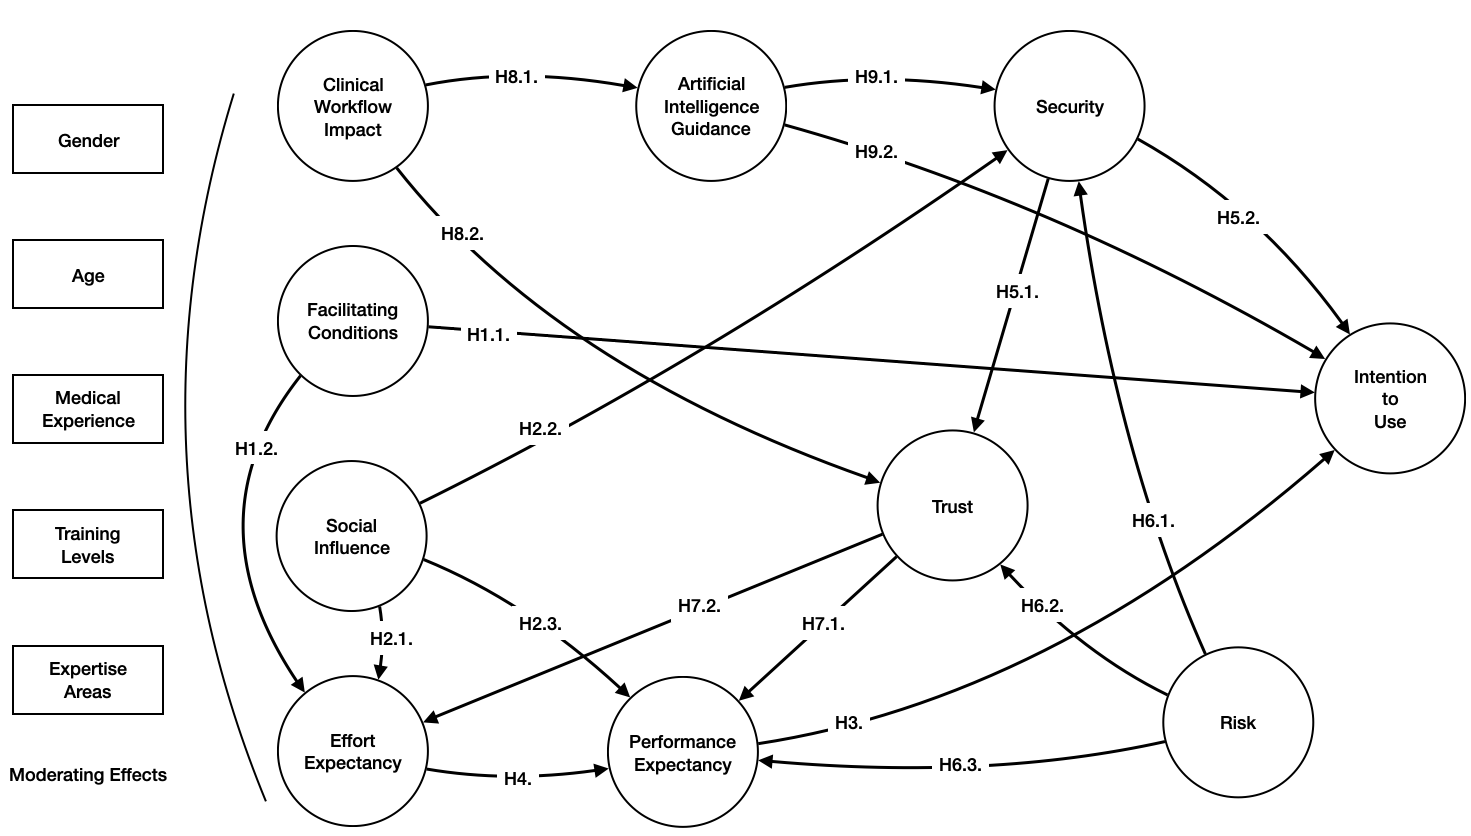
\includegraphics[width=\linewidth]{fig073}
\caption{\textcolor{revised}{The proposed research model, comparing the relations between moderating effects, model constructs, and hypotheses. We adapted this proposed research model from the UTAUT theoretical model to explain the actual adoption of AI in the medical imaging workflow. The research model includes 10 factors. We measured each factor with multiple items. Moreover, we adapted all items from extant literature to improve content validity.}}
\label{fig:fig073}
\end{figure}
%%%%%%%%%%%%%%%%%%%%%%%%%%%%%%%%%%%%%%%%%%%%%%%%%%%

\section{Research Questions \& Hypotheses}
\label{sec:chap004003}

\textcolor{revised}{In this study, we developed a questionnaire grounded in the \ac{UTAUT} model (Figure~\ref{fig:fig073}), which was meticulously adapted to address the unique context of \ac{AI} systems in medical imaging.
This adaptation involved integrating key variables such as trust, perceived usefulness, ease of use, security, risk, and social influence, with a particular emphasis on the nuances of \ac{AI} in the healthcare domain~\cite{BOOTSMAN201999}.
The primary objective was to explore the multifaceted impact of \ac{AI} on technology adoption, delving into aspects such as risk, privacy, and trust, which are critical in the medical imaging context.
Our approach aimed to enhance the questionnaire's explanatory power (Appendix~\ref{chap:app006}), making it more relevant and applicable across diverse \ac{AI} and \ac{HCI} scenarios.}

\textcolor{revised}{To ensure a robust and contextually relevant framework, we formulated hypotheses directly derived from the \ac{UTAUT} constructs, while also integrating insights from contemporary literature on trust, bias, and the explainability of \ac{AI} systems in healthcare~\cite{CHOUDHURY2022103708}.
This approach allowed us to construct a conceptual framework tailored for our exploratory study, focusing specifically on the core determinants of \ac{AI} adoption in medical imaging.
The model was designed to facilitate a nuanced analysis of moderator uncertainties and their potential impacts on these determinants.
The choice of \ac{UTAUT} as our theoretical foundation was informed by its empirical robustness and adaptability, particularly in the context of emerging technologies like \ac{AI} in healthcare settings~\cite{CALISTO2022102922}.
This alignment with the \ac{UTAUT} model, enriched with current literature, ensures that our study not only investigates general adoption patterns but also addresses specific challenges and considerations inherent to \ac{AI}-powered medical imaging systems.}

\subsection{Items Based on UTAUT Constructs}
\label{sec:chap004003001}

Our study takes an exploratory approach to hypothesize the significant effects on user adoption, drawing from the original \ac{UTAUT} constructs.
With these hypotheses, we propose a conceptual framework for our empirical study.
Our model not only covers the core determinants of \ac{AI} adoption, including intention and actual adoption, but also enables the research community to analyze moderator uncertainty that may constrain the effects of these determinants.
Based on its empirical superiority over other models~\cite{CALISTO2022102922}, we choose \ac{UTAUT} as the theoretical foundation for developing our hypotheses.

\vspace{2.00mm}

\noindent
Before describing the hypothesis, let us define {\it behavioral intention} in the context of this thesis:

\vspace{2.00mm}

\textcolor{revised}{{\it Behavioral Intention} is crucial for \ac{AI} tool adoption, reflecting clinicians' willingness to integrate these technologies~\cite{doi:10.1057/ejis.2012.15}.
Influenced by attitudes towards technology, beliefs about \ac{AI}'s efficacy, and the clinical environment, this intention links with trust in the \ac{AI} system, perceptions of biases, and transparency~\cite{Venkatesh2022}.
These factors shape clinicians' readiness to use \ac{AI}, indicating likely usage.
Understanding and influencing this intention bridges theoretical acceptance and practical application, guiding strategies to enhance \ac{AI} acceptance and improve patient care and diagnostic accuracy.}

% \vspace{2.00mm}

\noindent
From here, we specifically developed the following hypotheses:

\vspace{2.00mm}

\textcolor{revised}{{\it Facilitating Conditions} have direct positive relations with user behavior but no effect on behavioral intentions~\cite{CALISTO2022102922}.
Although other authors are using the original \ac{UTAUT} model with separate constructs~\cite{KHALILZADEH2017460}, in this study, we are using behavioral intention as a proxy for user behavior.
In this thesis, it refers to the external factors or circumstances that can either support or hinder a clinician's ability to perform a specific behavior or adopt \ac{AI} technology.}

\vspace{2.00mm}

\noindent
Hence, we hypothesize that:

\vspace{2.00mm}

\noindent
{\bf H1.1.} The facilitating conditions for using \ac{AI} in the clinical workflow, positively predict users' intentions to use it;

\vspace{2.00mm}

\noindent
{\bf H1.2.} The facilitating conditions ({\it e.g.}, ability to use the system) for using \ac{AI} in the clinical workflow, has a direct positive impact on effort expectancy;

\vspace{2.00mm}

{\it Social Influence} has direct impact on behavioral intention.
The underlying assumption is that clinicians tend to consult their medical community about novel diagnosis paradigms and can be influenced by perceived social pressure.
Because perceived security also involves a patient's health for misdiagnosing the case, it should be highly influenced in the proposed model.

\vspace{2.00mm}

\noindent
Based on this, we anticipate that:

\vspace{2.00mm}

\noindent
{\bf H2.1.} The social influence ({\it e.g.}, recommendations from the medical community) for using an \ac{AI} system, positively predicts effort expectancy;

\vspace{2.00mm}

\noindent
{\bf H2.2.} The social influence of using an \ac{AI} system, positively and directly influences perceived security;

\vspace{2.00mm}

\noindent
{\bf H2.3.} The social influence of using an \ac{AI} system, has a direct positive impact on performance expectancy;

\vspace{2.00mm}

{\it Performance Expectancy} is a strong predictor of behavioral intention~\cite{KHALILZADEH2017460}.
It can be divided into utilitarian performance expectancy and hedonic performance expectancy~\cite{CALISTO2022102922}.
While enhancing task performance can increase satisfaction, the effect of hedonic motivation may be weaker, according to some authors~\cite{HART201993}.
In radiology, the ability of \ac{AI} to provide an autonomous second reader that supports decision-making is an attractive goal, offering practical benefits likely to drive adoption.

\vspace{2.00mm}

\noindent
Therefore, we hypothesize that:

\vspace{2.00mm}

\noindent
{\bf H3.} Performance expectancy ({\it i.e.}, usefulness) positively affects behavioral intention to use an \ac{AI} system;

\vspace{2.00mm}

{\it Effort Expectancy} is another predictor of intention to use \ac{AI} systems~\cite{CALISTO2022102922}.
Several authors also find effort expectancy to affect behavioral intention significantly~\cite{KHALILZADEH2017460, HART201993}.
As \ac{AI} provides a new paradigm shift, the perceived degree of ease associated with \ac{AI} systems will likely affect behavioral intention.

% \vspace{2.00mm}

\noindent
In accordance, we denote that:

\vspace{2.00mm}

\noindent
{\bf H4.} Effort expectancy ({\it i.e.}, ease of use) positively affects performance expectancy ({\it i.e.}, usefulness) to use \ac{AI} systems;

% \vspace{2.00mm}

\subsection{Items Based on UTAUT Extensions}
\label{sec:chap004003002}

Trust, security, and risk are pivotal in general technology adoption and play a significant role in sensitive areas like healthcare~\cite{KHALILZADEH2017460}.
The reluctance of clinicians to integrate new technologies in disseminating medical information highlights the need for robust security measures and trust-building strategies to mitigate perceived risks~\cite{10.1145/3132272.3134111}.
This is further emphasized by the increasing concerns about data privacy and the potential misuse of sensitive health information in the digital era~\cite{CALISTO2022102922}.

\vspace{2.00mm}

{\it Perceived Security} is expected to affect behavioral intention directly.
Because \ac{AI} systems involve sensitive patient information, it should be highly influential in the proposed model~\cite{KHALILZADEH2017460}.
Moreover, perceived security is an aggregating construct, changing over time according to medical experts' community opinion and social influence.

\vspace{2.00mm}

\noindent
Therefore, we hypothesize that:

\vspace{2.00mm}

\noindent
{\bf H5.1.} Perceived security of \ac{AI} systems positively and directly predicts perceived trust;

\vspace{2.00mm}

\noindent
{\bf H5.2.} Perceived security of \ac{AI} systems positively and directly behavioral intention to use \ac{AI} systems;

\vspace{2.00mm}

{\it Perceived Risk} is usually related to perceived security.
The more a user perceives the risk, the less secure the user's feel, leading to a negative relationship between risk and security~\cite{KHALILZADEH2017460}.
Indeed, the literature~\cite{10.1145/3132272.3134111, HART201993} states that perceived risk has negative impact on perceived security, and trust, as well as performance expectancy.

\vspace{2.00mm}

\noindent
Based on these literature findings, we formulate the following hypothesis:

\vspace{2.00mm}

\noindent
{\bf H6.1.} The perceived risk of using \ac{AI} systems has a direct negative impact on perceived security;

\vspace{2.00mm}

\noindent
{\bf H6.2.} The perceived risk of using \ac{AI} systems has a direct negative impact on perceived trust;

\vspace{2.00mm}

\noindent
{\bf H6.3.} The perceived risk of using \ac{AI} systems has a direct negative impact on performance expectancy;

\vspace{2.00mm}

{\it Trust} positively affects behavioral intentions~\cite{HART201993}.
As a unitary construct, the effect of trust on behavioral intention has gained notable support.
Moreover, this construct is the most significant predictor of behavioral intention~\cite{CALISTO2022102922, HART201993}.
While \ac{AI}-based solutions become ubiquitous, trust supersedes the importance of traditional adoption factors such as perceived usefulness.
Akin to Khalilzadeh et al.~\cite{KHALILZADEH2017460}, this study includes trust as a singular construct, which is likely to be critical due to the novelty of \ac{AI} systems in the medical workflow and complex environments.

% \vspace{2.00mm}

\noindent
Thus, we hypothesize that:

\vspace{2.00mm}

\noindent
{\bf H7.1.} Trust positively affects performance expectancy ({\it i.e.}, usefulness) to use \ac{AI} systems;

\vspace{2.00mm}

\noindent
{\bf H7.2.} Trust positively affects effort expectancy ({\it i.e.}, ease of use) to use \ac{AI} systems;

% \vspace{2.00mm}

\subsection{Items Related to Impact}
\label{sec:chap004003003}

\ac{AI} has a significant social and personal behavioral impact on the medical community all over the world~\cite{CALISTO2022102922}.
Medical diagnosis impacts significantly on people's health and peoples' lives, and clinicians have to take responsibility for their actions.
Therefore, clinicians may be more cautious than professionals in other fields when considering adopting new technologies to assist their work.
Although clinicians typically resist new technologies, several authors~\cite{doi:10.1148/ryai.2020190043, WAYMEL2019327} are reporting a new behavior change for adopting \ac{AI} systems in the clinical workflow, whereas these systems are increasing clinicians' performance during decision-making \cite{CALISTO2021102607}.

As introduced in Section~\ref{sec:chap004002}, the \ac{TRA} inspires various technology adoption models, arguing that both attitudes toward an action and subjective norms have an impact on behavioral intention, affecting how people perform an action~\cite{CALISTO2022102922}.
Adapted from \ac{TRA} and \ac{TAM}, the \ac{UTAUT} definition of attitude through behavior is ``{\it an individual's positive feeling about performing the target behavior}''~\cite{KHALILZADEH2017460}.
On the other hand, subjective norm refers to ``{\it a person's perception that most people who are important to them think they should or should not perform the behavior in question}''~\cite{WAYMEL2019327}.
\textcolor{revised}{Understanding trust and risk perception is vital for healthcare \ac{AI} integration~\cite{CHOUDHURY2022103708}, with diversity in medical practices and cultural contexts impacting its use in various environments~\cite{Lambert2023}.
Crucial for trust and risk management, diversity in institutional policies and cultural attitudes affects \ac{AI} adoption, effectiveness, and interpretation.}

\vspace{2.00mm}

\noindent
Hence, we hypothesize that:

\vspace{2.00mm}

\noindent
{\bf H8.1.} The extent to which \ac{AI} positively impacts the clinical workflow due to better decision-making of clinicians ({\it e.g.}, decreasing the medical error, time-to-diagnose, etc.), affects the intention to follow \ac{AI} guidance ({\it i.e.}, preferring a timely and less prone to medical error \ac{AI} second-reader);

\vspace{2.00mm}

\noindent
{\bf H8.2.} The extent to which \ac{AI} positively impacts the clinical workflow ({\it e.g.}, decreasing the medical error, time-to-diagnose, etc.) due to better decision-making of clinicians, directly predicts perceived trust;

\vspace{2.00mm}

\textcolor{revised}{Salient beliefs and evaluations shape clinicians' intentions to follow \ac{AI} guidance, but these may not align with factors driving their actual use of \ac{AI}\cite{KHALILZADEH2017460}.
Studies indicate a strong link between trust, perceived risk, and behavioral intentions\cite{GANSSER2021101535, WAYMEL2019327}, yet trust's impact on risk perception does not always translate into actual compliance.
Concerns arise, especially in context-aware applications where \ac{AI} processes subjective data~\cite{10.1145/3313831.3376506}.
This highlights a complex interplay among trust, risk, and compliance in \ac{AI} applications in healthcare settings.}

\textcolor{revised}{Within the \ac{UTAUT} model, our research further explores these dynamics, focusing on what motivates clinicians to follow \ac{AI} guidance in real-world scenarios.
In short, our goal is to investigate how perceived ease of use, performance expectations, and social influence shape clinicians' attitudes towards \ac{AI} adoption.
Additionally, we aim to examine the role of professional experience and specialty in modulating these motivations, recognizing that different medical fields may exhibit varied responses to \ac{AI} integration.
Our study also seeks to understand the threshold at which perceived advantages of \ac{AI} guidance outweigh any reservations, thereby identifying key leverage points for facilitating wider acceptance and effective use of \ac{AI} in medical diagnostics.}

\textcolor{revised}{Existing studies have not explicitly differentiated between factors influencing `intention to follow \ac{AI} guidance' and those affecting clinicians’ actual adherence~\cite{AMEEN2021106548}.
Clinicians may express willingness to adhere to \ac{AI} recommendations, perceiving that the advantages surpass potential risks and security concerns.
However, their actual compliance often hinges on practical factors such as the \ac{AI}'s reliability and organizational policies~\cite{JURAVLE2020263}.
Trust primarily shapes clinicians' willingness and intention, while factors like \ac{AI} performance, security, and institutional norms are more pivotal in their actual decision to follow \ac{AI} guidance.
Therefore, understanding the intricate relationship between trust, intention, and compliance is crucial in designing effective strategies to promote clinicians' acceptance and adherence to \ac{AI} guidance.}

\vspace{2.00mm}

\noindent
Given the wide applicability of \ac{UTAUT}, we can anticipate that:

\vspace{2.00mm}

\noindent
{\bf H9.1.} The willingness to follow the \ac{AI} guidance positively and directly influences perceived security;

\vspace{2.00mm}

\noindent
{\bf H9.2.} The willingness to follow the \ac{AI} guidance positively affects the intention to use AI systems;

% \vspace{2.00mm}

\section{Methods}
\label{sec:chap004004}

Our research model includes ten constructs.
For this study, we measured each construct with multiple items (Figure~\ref{fig:fig075}).
To preserve the content validity and reliability, we measured most of our items from the extant literature~\cite{SOHN2020101324}.
From here, we adjusted these items in our questionnaire to match the context of \ac{AI} adoption among clinicians.
In compliance with recommendations of the two-stage analytical procedure, we used \ac{CFA} to test the measurement model’s validity and reliability~\cite{2019-07124-034}.
In addition, we used \ac{SEM} as a preferable technique to regression.
It allows simultaneous analysis of all relationships through multiple regression, while also allowing for both observed and latent variables to be analyzed simultaneously and providing overall fit statistics.
We conducted \ac{CFA} using the \texttt{R language} (\texttt{v 4.0.2}) employing \ac{MLE}.
Furthermore, \ac{MLE} was then followed by path analysis of the structural relationships conducted in the \texttt{R language} with \ac{SEM} libraries (\texttt{lavaan v. 0.6-7} and \texttt{semTools v. 0.5-3}).
We also undertook moderation analysis in the \texttt{R} language.

%%%%%%%%%%%%%%%%%%%%%%%%%%%%%%%%%%%%%%%%%%%%%%%%%%%
\begin{figure}[htpb]
\centering
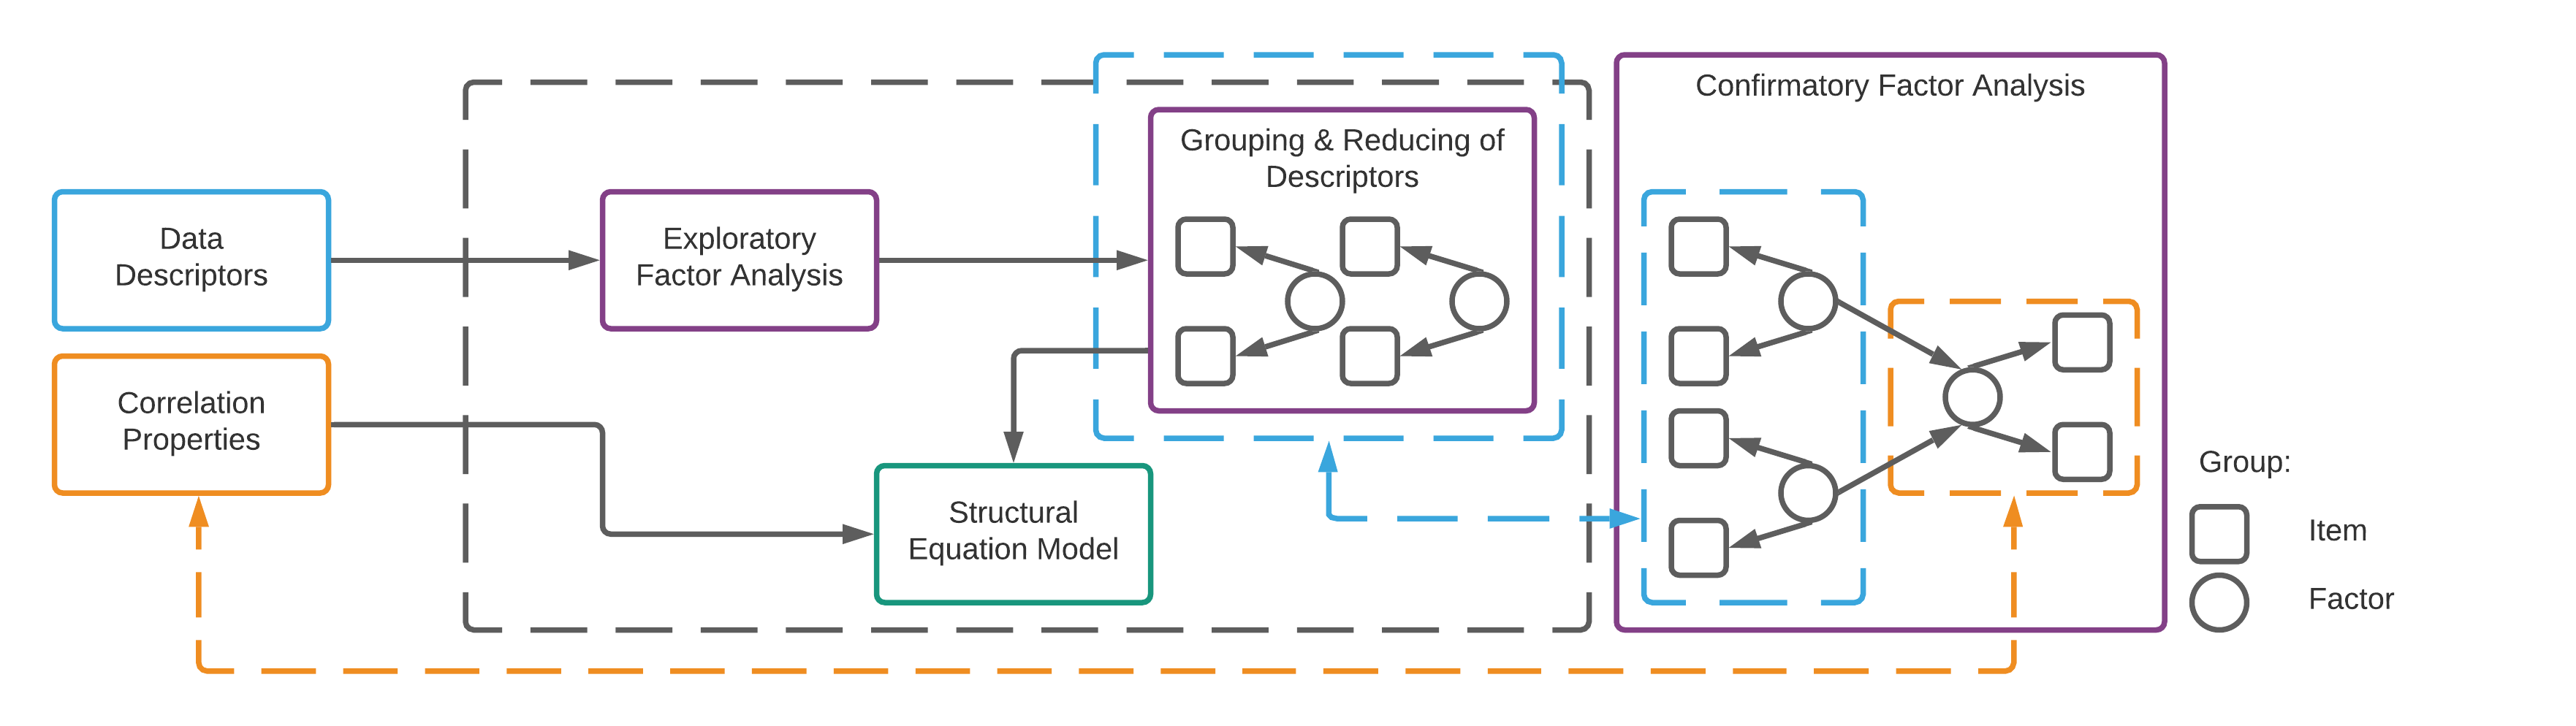
\includegraphics[width=0.985\linewidth]{fig075}
\caption{The basic statistical flow steps followed by us are usually taken in the framework of SEM modeling. Before employing the SEM modeling, we used the conceptual EFA to reduce and group descriptors. Here, we identified the latent factors by using the CFA. Finally, we applied the SEM to estimate the coefficients.}
\label{fig:fig075}
\end{figure}
%%%%%%%%%%%%%%%%%%%%%%%%%%%%%%%%%%%%%%%%%%%%%%%%%%%

\subsection{Procedures}
\label{sec:chap004004001}

We sent the questionnaire via social media ({\it e.g.}, radiology groups on Facebook and LinkedIn) to 17203 participants who gave prior permission to use their data for research purposes under this international study.
The questionnaire contained i) a general explanation of the study, ii) the details of the privacy policy, iii) data treatment, and a iv) link to a Google Forms survey (Appendix~\ref{chap:app006}).
We sent the questionnaire in the middle of February 2021.
The criterion was to send the questionnaire to clinicians worldwide who are members of these social media target groups ({\it i.e.}, radiologists, physicians from any other expertise, technicians, etc.).
Overall, this procedure remained until the end of July 2021, when we analysed and discussed our data.

\subsection{Participants}
\label{sec:chap004004002}

\textcolor{revised}{Table~\ref{tab:tab008}} is listing the sample demographics under this study.
In total, we collected data from 322 participants, corresponding to an overall participation of 1.9\%.
Regarding general demographics (N = 322), the sample consisted of a slightly higher proportion of men (59.9\%) than women (38.8\%) with 1.2\% answering ``Prefer not to say'' during the questionnaire.
For age groups, 12.1\% of participants range from 18 to 29 years old, 29.5\% from 30 to 39, 22.7\% from 40 to 49, 23.9\% from 50 to 59, 10.2\% older than 59, and 1.6 answering ``Prefer not to say'' during the questionnaire.

%%%%%%%%%%%%%%%%%%%%%%%%%%%%%%%%%%%%%%%%%%%%%%%%%%%
\begin{table}[htpb]
\resizebox{\columnwidth}{!}{%
\begin{tabular}{cccc}
\hline
\rule{0mm}{4mm}
Demographic                   & Group                    & Frequency & Percentage
\\
\hline
\multirow[t]{3}{*}{Gender}       & Female                    & 125       & 38.8\%     \\
                                 & Male                      & 193       & 59.9       \\
                                 & Other                     & 4         & 1.2        \\
\hline
\multirow[t]{6}{*}{Age}          & 18 - 29                  & 39        & 12.1\%     \\
                                 & 30 - 39                  & 95        & 29.5\%     \\
                                 & 40 - 49                  & 73        & 22.7\%     \\
                                 & 50 - 59                  & 77        & 23.9\%     \\
                                 & > 59                     & 33        & 10.2\%     \\
                                 & N.A.                     & 5         & 1.6\%      \\
\hline
\multirow[t]{7}{*}{Nationality}  & Europe                   & 126       & 39.2\%     \\
                                 & North America            & 82        & 25.5\%     \\
                                 & Africa                   & 36        & 11.2\%     \\
                                 & Middle East              & 26        & 8.1\%      \\
                                 & Asia                     & 24        & 7.5\%      \\
                                 & Central \& South America & 19        & 5.9\%      \\
                                 & Oceania                  & 9         & 2.8\%      \\
\hline
\multirow[t]{5}{*}{Education}    & Specialists              & 111       & 34.5\%     \\
                                 & Bachelor                 & 81        & 25.2\%     \\
                                 & Master                   & 78        & 24.2\%     \\
                                 & PhD                      & 45        & 14\%       \\
                                 & N.A.                     & 7         & 2.1\%      \\
\hline
\multirow[t]{5}{*}{Medical Experience} & Interns            & 24        & 7.5\%      \\
                                       & Juniors            & 26        & 8.1\%      \\
                                       & Middles            & 54        & 16.5\%     \\
                                       & Seniors            & 210       & 65.2\%     \\
                                       & N.A.               & 8         & 2.4\%      \\
\hline
\multirow[t]{3}{*}{Training Levels}    & Doctors            & 132       & 41\%       \\
                                       & Technicians        & 105       & 32.6\%     \\
                                       & Other              & 85        & 26.4\%     \\
\hline
\end{tabular}%
}
\caption{Characteristics of participants for demographic groups with frequency and percentage. The main characteristics are gender, age, nationality, and education.}
\label{tab:tab008}
\end{table}
%%%%%%%%%%%%%%%%%%%%%%%%%%%%%%%%%%%%%%%%%%%%%%%%%%%

Other demographic data add fundamental insights to this study, such as the medical experience of participants (Section~\ref{chap:app002003001}), training levels (Section~\ref{chap:app002003002}), and expertise areas (Section~\ref{chap:app002003003}).
In this study, the education level of participants is also vital to denote relations between demographic data.
Specifically, 34.5\% of participants are specialists, 25.2\% have at least one bachelor's degree, 24.2\% have a \ac{MSc}, and 14\% have a \ac{PhD} degree.
The other 2.1\% are typically students or academic associate degrees.

\section{Results}
\label{sec:chap004005}

In this study, we examined the sample characteristics of participants (Section~\ref{chap:app002003} of Appendix~\ref{chap:app002}) to gain insights into their profiles and experiences in the medical imaging domain.
\textcolor{revised}{Above, Table~\ref{tab:tab008} presents an overview of these characteristics, shedding light on the typical participant in this study.}
The findings reveal that the typical participant is a radiology specialist in the mid-career stage, primarily working in the public sector.
Most clinicians engage in the analysis of medical imaging exams regularly, with a majority analyzing patients daily.
Furthermore, participants demonstrate varying familiarity with \ac{AI} systems, ranging from awareness without usage to regular utilization.
These insights into the participants' profiles and experiences provide valuable context for understanding their perspectives and behaviors in adopting \ac{AI} technology in healthcare settings.
For a comprehensive summary of all these results, please refer to Section~\ref{chap:app002004006} of Appendix~\ref{chap:app002}.

\subsection{Checking Assumptions}
\label{sec:chap004005001}

The assumptions of the \ac{SEM} were met in this study (Section~\ref{chap:app002004001} of Appendix~\ref{chap:app002}), with normal distributions observed for all variables~\cite{CALISTO2022102922}.
The overall model fit was good~\cite{doi:10.1504/IJMDA.2017.087624}, as indicated by \acp{GFI} of 0.824 surpassing the recommended thresholds.
While some indices were slightly below the recommended levels, the literature suggests that sample size can impact these fit indices~\cite{doi:10.1080/00273171.2019.1602503}.
Notably, the ratio of the test statistic ($\chi^2$) to the degree of freedom ($df$) was within the recommended range ($\chi^2$ / $df$ = 2.587 $<$ 3.0), and both \ac{RMSEA} and \ac{SRMR} of 0.083 indicated an acceptable model fit~\cite{ZHOU2010760}.
Despite a significant $\chi^2$ value due to the large sample size, the Hoelter index confirmed that the sample adequately supported the sophisticated model~\cite{CALISTO2022102922}.

\subsection{Measurement Model}
\label{sec:chap004005002}

Convergent and discriminant validity were examined to ensure the robustness of the measurement model~\cite{CALISTO2022102922}.
All item loadings were significant (p-value = 0.000), indicating good convergent validity, with most loadings above 0.8~\cite{CALISTO2022102922}.
Each item significantly loaded on its respective construct, demonstrating convergent validity.
Discriminant validity was confirmed by comparing shared variance and \ac{AVE}, with shared variance lower than \ac{AVE}.
The measurement model exhibited good reliability, with a \ac{CR} of 0.95~\cite{doi:10.1504/IJMDA.2017.087624}.
These findings confirm the reliability, convergent validity, and discriminant validity of the measurement model.
Moderating effects on other variables (Section~\ref{sec:chap004005005}), particularly demographics, warrant further investigation.
\textcolor{revised}{Comprehensive findings from the \ac{CFA} are detailed in Table~\ref{tab:tab009}.
For an in-depth analysis, additional information and expanded results of the \ac{CFA} can be found in Section~\ref{chap:app002004002} of Appendix~\ref{chap:app002}.}

%%%%%%%%%%%%%%%%%%%%%%%%%%%%%%%%%%%%%%%%%%%%%%%%%%%
\begin{table*}
\resizebox{\textwidth}{!}{%
\begin{tabular}{ccccccccccc}
\hline
Measure & Impact & Guidance & PerfExp & EffExp & SocInf & FacCond & IntUse & Security & Risk & Trust \\ \hline
alpha   & 0.57   & 0.88     & 0.87    & 0.89   & 0.73   & 0.80    & 0.94   & 0.83     & 0.84    & 0.88  \\
CR      & 0.57   & 0.88     & 0.89    & 0.89   & 0.74   & 0.79    & 0.93   & 0.82     & 0.84    & 0.88  \\
AVE     & 0.40   & 0.65     & 0.72    & 0.73   & 0.49   & 0.55    & 0.78   & 0.60     & 0.64    & 0.70  \\ \hline
\end{tabular}%
}
\caption{The abbreviated constructs are as follows: Clinical Workflow Impact (Impact); AI Guidance (Guidance); Performance Expectancy (PerfExp); Effort Expectancy (EffExp); Social Influence (SocInf); Facilitating Conditions (FacCond); Behavior Intention to Use (IntUse); Perceived Security (Security); Perceived Risk (Risk); Perceived Trust (Trust). Moreover, the measure abbreviations are: Cronbach alpha (alpha); Composite Reliability (CR); Average Variance Extracted (AVE).}
\label{tab:tab009}
\end{table*}
%%%%%%%%%%%%%%%%%%%%%%%%%%%%%%%%%%%%%%%%%%%%%%%%%%%

\subsection{Parallel Analysis}
\label{sec:chap004005003}

Parallel analysis was conducted to determine the appropriate number of factors to retain in the measurement model~\cite{doi:10.1080/10705511.2019.1615835}.
By simulating eigenvalues based on the number of items and sample size, the parallel analysis compares these simulated eigenvalues with the eigenvalues obtained from the study \textcolor{revised}{(Figure~\ref{fig:fig093})}.
Factors with eigenvalues that overlap with the cutoff line for retention indicate potential factors to consider.
The scree plot in \textcolor{revised}{Figure~\ref{fig:fig093}} shows notable changes in effect size, suggesting a breakpoint for the number of factors.
However, the decision to retain factors is not solely based on these changes; it also considers the line limits of the parallel analysis.

%%%%%%%%%%%%%%%%%%%%%%%%%%%%%%%%%%%%%%%%%%%%%%%%%%%
\begin{figure}[htpb]
\centering
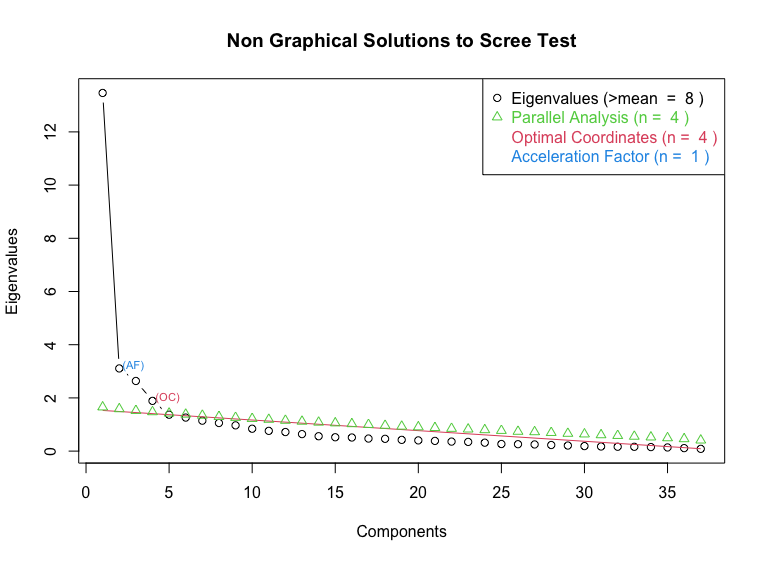
\includegraphics[width=0.955\linewidth]{fig093}
\caption{\textcolor{revised}{Scree plot of eigenvalues with the eigenvalues greater than one rule, elbow bend, and intersecting lines.}}
\label{fig:fig093}
\end{figure}
%%%%%%%%%%%%%%%%%%%%%%%%%%%%%%%%%%%%%%%%%%%%%%%%%%%

The difference in eigenvalues becomes more significant when comparing the fifth and sixth components, as well as the sixth and seventh components.
Components eight and nine are mainly below the line, highlighting the arbitrary nature of item retention for factors or overall models~\cite{CALISTO2022102922}.
Therefore, the analysis suggests retaining factors up to the seventh component, resulting in a total of seven factors in the measurement model.
More details on the parallel analysis results will be described in Section~\ref{chap:app002004003} of Appendix~\ref{chap:app002}.

\subsection{Structural Model}
\label{sec:chap004005004}

The satisfactory fit of the measurement model allowed us to employ \ac{SEM} for data analysis.
\ac{SEM} evaluates the extent to which the collected data align with the theoretical model's measurement~\cite{doi:10.1080/10705511.2017.1401932}.
In this study, we extended the proposed research model by introducing two new constructs:
(1) Clinical Workflow Impact; and
(2) \ac{AI} Guidance.
These additions enabled us to explore the interactions between these constructs and existing variables within the model.
We assessed the structural relationships by estimating the hypothesized causal paths, with the majority of hypotheses supported (except for {\bf H6.1}, {\bf H6.3}, and {\bf H7.1}) based on a significance level of {\it p-value} $<$ 0.10 from \textcolor{revised}{Table~\ref{tab:tab011}}.
For a more comprehensive analysis of \ac{SEM} and its evaluation, refer to Section~\ref{chap:app002004004} of Appendix~\ref{chap:app002}.
This section provides detailed insights into the relationships between variables \textcolor{revised}{(Table~\ref{tab:tab010})}, further supporting our findings.

%%%%%%%%%%%%%%%%%%%%%%%%%%%%%%%%%%%%%%%%%%%%%%%%%%%
\begin{table}[htpb]
\resizebox{\columnwidth}{!}{%
\begin{tabular}{lrrrrrl}
\hline
Hypotheses & \multicolumn{1}{l}{b} & \multicolumn{1}{l}{StdError} & \multicolumn{1}{l}{z-value} & \multicolumn{1}{l}{p-value} & \multicolumn{1}{l}{beta} & Supported \\
\hline
\textbf{H1.1.} & 0.313  & 0.053 & 5.912  & 0.000 & 0.349  & Yes ***                  \\
\textbf{H1.2.} & 0.432  & 0.08  & 5.393  & 0.000 & 0.375  & Yes ***                  \\
\textbf{H2.1.} & 0.268  & 0.133 & 2.015  & 0.044 & 0.211  & Yes **                   \\
\textbf{H2.2.} & 0.432  & 0.08  & 5.393  & 0.000 & 0.375  & Yes ***                  \\
\textbf{H2.3}  & 0.239  & 0.067 & 3.554  & 0.000 & 0.243  & Yes ***                  \\
\textbf{H3.}   & 0.327  & 0.068 & 4.81   & 0.000 & 0.264  & Yes ***                  \\
\textbf{H4.}   & 0.466  & 0.061 & 7.653  & 0.000 & 0.603  & Yes ***                  \\
\textbf{H5.1.} & 0.701  & 0.078 & 9.012  & 0.000 & 0.715  & Yes ***                  \\
\textbf{H5.2.} & 0.239  & 0.06  & 4.005  & 0.000 & 0.226  & Yes ***                  \\
\textbf{H6.1.} & -0.016 & 0.049 & -0.326 & 0.744 & -0.02  & \textcolor{red}{No}      \\
\textbf{H6.2.} & -0.098 & 0.059 & -1.672 & 0.095 & -0.124 & Yes *                    \\
\textbf{H6.3.} & -0.031 & 0.033 & -0.962 & 0.336 & -0.046 & \textcolor{red}{No}      \\
\textbf{H7.1.} & 0.009  & 0.045 & 0.197  & 0.844 & 0.01   & \textcolor{red}{No}      \\
\textbf{H7.2.} & 0.375  & 0.062 & 6.014  & 0.000 & 0.333  & Yes ***                  \\
\textbf{H8.1.} & -0.494 & 0.09  & -5.512 & 0.000 & -0.487 & Yes ***                  \\
\textbf{H8.2.} & 0.176  & 0.092 & 1.92   & 0.055 & 0.179  & Yes *                    \\
\textbf{H9.1.} & 0.459  & 0.067 & 6.861  & 0.000 & 0.464  & Yes ***                  \\
\textbf{H9.2.} & 0.336  & 0.055 & 6.151  & 0.000 & 0.322  & Yes ***                  \\
\hline
\end{tabular}%
}
\caption{Summary of hypothesis tests. The variables assigned to the significance values are as follows: *** significant at level $\alpha = 0.01$; ** significant at level $\alpha = 0.05$; and * significant fixed at level $\alpha = 0.10$.}
\label{tab:tab011}
\end{table}
%%%%%%%%%%%%%%%%%%%%%%%%%%%%%%%%%%%%%%%%%%%%%%%%%%%

\clearpage

%%%%%%%%%%%%%%%%%%%%%%%%%%%%%%%%%%%%%%%%%%%%%%%%%%%
\begin{table}[htpb]
\resizebox{\columnwidth}{!}{%
\begin{tabular}{llrrrl}
\hline
Construct                   & Item        & \multicolumn{1}{l}{Alpha} & \multicolumn{1}{l}{StdError} & \multicolumn{1}{l}{z-value} & p-value \\ \hline
Clinical Workflow Impact & Impact\_1   & 0.53 & 0.080 & 6.615  & 0.000 \\
Alpha = 0.57                & Impact\_2   & 0.75  & 0.079    & 9.499   & 0.000   \\ \hline
AI Guidance              & Guidance\_1 & 0.36 & 0.035 & 10.209 & 0.000 \\
Alpha = 0.88             & Guidance\_2 & 0.29 & 0.028 & 10.102 & 0.000 \\
R2 = 0.238                  & Guidance\_3 & 0.19  & 0.026    & 7.262   & 0.000   \\
                            & Guidance\_4 & 0.32  & 0.033    & 9.683   & 0.000   \\ \hline
Performance Expectancy      & PerfExp\_1  & 0.45                      & 0.039                        & 11.606                      & 0.000   \\
Alpha = 0.87                & PerfExp\_2  & 0.14                      & 0.019                        & 7.186                       & 0.000   \\
R2 = 0.595                  & PerfExp\_3  & 0.08                      & 0.018                        & 4.382                       & 0.000   \\ \hline
Effort Expectancy           & EffExp\_1   & 0.16                      & 0.022                        & 7.335                       & 0.000   \\
Alpha = 0.89                & EffExp\_2   & 0.19                      & 0.021                        & 8.615                       & 0.000   \\
R2 = 0.496                  & EffExp\_3   & 0.25                      & 0.025                        & 9.821                       & 0.000   \\ \hline
Social Influence            & SocInf\_1   & 0.57                      & 0.054                        & 10.464                      & 0.000   \\
Alpha = 0.73                & SocInf\_2   & 0.68                      & 0.066                        & 10.24                       & 0.000   \\
                            & SocInf\_3   & 0.35                      & 0.047                        & 7.356                       & 0.000   \\ \hline
Facilitating Conditions     & FacCond\_1  & 0.56                      & 0.06                         & 9.284                       & 0.000   \\
Alpha = 0.80                & FacCond\_2  & 0.57                      & 0.061                        & 9.45                        & 0.000   \\
                            & FacCond\_3  & 0.41                      & 0.046                        & 8.932                       & 0.000   \\ \hline
Behavioral Intention to Use & IntUse\_1   & 0.16                      & 0.017                        & 9.576                       & 0.000   \\
Alpha = 0.94                & IntUse\_2   & 0.13                      & 0.015                        & 8.496                       & 0.000   \\
R2 = 0.681                  & IntUse\_3   & 0.15                      & 0.016                        & 9.761                       & 0.000   \\
                            & IntUse\_4   & 0.19                      & 0.019                        & 9.856                       & 0.000   \\ \hline
Security                    & Security\_1 & 0.41                      & 0.041                        & 10.055                      & 0.000   \\
Alpha = 0.83                & Security\_2 & 0.14                      & 0.025                        & 5.621                       & 0.000   \\
R2 = 0.397                  & Security\_3 & 0.39                      & 0.037                        & 10.537                      & 0.000   \\ \hline
Risk                        & Risk\_1  & 0.36                         & 0.049                        & 7.342                       & 0.000   \\
Alpha = 0.84                & Risk\_2  & 0.57                         & 0.06                         & 9.48                        & 0.000   \\
                            & Risk\_3  & 0.34                         & 0.047                        & 7.114                       & 0.000   \\ \hline
Trust                       & Trust\_1    & 0.30                      & 0.031                        & 9.762                       & 0.000   \\
Alpha = 0.88                & Trust\_2    & 0.19                      & 0.025                        & 7.606                       & 0.000   \\
R2 = 0.465                  & Trust\_3    & 0.21                      & 0.029                        & 7.385                       & 0.000  \\ \hline
\end{tabular}%
}
\caption{The measuring model with: Clinical Workflow Impact ({\bf Impact}); AI Guidance ({\bf Guidance}); Performance Expectancy ({\bf PerfExp}); Effort Expectancy ({\bf EffExp}); Social Influence ({\bf SocInf}); Facilitating Conditions ({\bf FacCond}); Behavioral Intention to Use ({\bf IntUse}); {\bf Security}; {\bf Risk}; and {\bf Trust}. The computed measurements are {\bf Alpha}, Standard Error ({\bf StdError}), {\bf z-value}, and {\bf p-value}.}
\label{tab:tab010}
\end{table}
%%%%%%%%%%%%%%%%%%%%%%%%%%%%%%%%%%%%%%%%%%%%%%%%%%%

\clearpage

The coefficient of determination ($R^2$), also known as \ac{SMC}, provides insights into the explanatory power and predictive accuracy of the measurement model \textcolor{revised}{(Table~\ref{tab:tab010})}.
Higher loadings indicate stronger relationships between the items and their corresponding latent constructs.
\textcolor{revised}{In the context of the \ac{UTAUT} model, a high $R^2$ value indicates an effective capture of variance in user acceptance and technology usage behavior.
This is vital for validating the model's robustness and assessing the impact of its constructs on technology adoption.}

Behavioral intention exhibited the highest value ($R^2$ = 0.681), indicating a substantial amount of variance explained.
Conversely, \ac{AI} Guidance had the lowest value ($R^2$ = 0.238), followed by security ($R^2$ = 0.397).
These lower values can be attributed to their close association with independent variables and the inherent nature of the constructs, which are influenced by a clinician's belief in \ac{AI} systems.
The coefficient for performance expectancy ($R^2$ = 0.595), effort expectancy ($R^2$ = 0.496), and trust ($R^2$ = 0.465) were also acceptable, which is consistent with previous results~\cite{KHALILZADEH2017460}.
These coefficients indicate the extent to which the independent variables can account for the variance in the dependent variable.

\subsection{Moderating Effects}
\label{sec:chap004005005}

To examine potential moderator effects, we conducted a comprehensive analysis using the split sample approach \cite{LI2021106581, LI2021106929}.
We investigated the moderation of gender, age, nationality, education, and clinical knowledge on the relationships within our research model.
Notably, significant moderating effects were found for all variables, providing insights into the nuanced dynamics and contextual influences within the model.
The detailed results are presented in Table~\ref{tab:tab012}, which includes the path coefficients and significance levels for each moderator variable.
These findings underscore the importance of considering demographic factors in understanding the relationships in our study.

%%%%%%%%%%%%%%%%%%%%%%%%%%%%%%%%%%%%%%%%%%%%%%%%%%%
\begin{table}[htpb]
\resizebox{\textwidth}{!}{%
\begin{tabular}{|l|ll|ll|ll|ll|ll|}
\hline
\multicolumn{1}{|c|}{\multirow{2}{*}{Hypotheses}} &
  \multicolumn{2}{c|}{Gender} &
  \multicolumn{2}{c|}{Age} &
  \multicolumn{2}{c|}{Nationality Classification} &
  \multicolumn{2}{c|}{Education} &
  \multicolumn{2}{c|}{Knowledge} \\ \cline{2-11} 
\multicolumn{1}{|c|}{} &
  \multicolumn{1}{c|}{Woman} &
  \multicolumn{1}{c|}{Man} &
  \multicolumn{1}{c|}{\textless 30} &
  \multicolumn{1}{c|}{\textgreater{}= 30} &
  \multicolumn{1}{c|}{Developed} &
  \multicolumn{1}{c|}{Developing} &
  \multicolumn{1}{c|}{Higher} &
  \multicolumn{1}{c|}{Advanced} &
  \multicolumn{1}{c|}{Expert} &
  \multicolumn{1}{c|}{Novice} \\ \hline
\textbf{H1.1.} &
  \multicolumn{1}{l|}{$\textcolor{red}{\downarrow}$ 0.39 ***} &
  $\textcolor{blue}{\uparrow}$ 0.64 *** &
  \multicolumn{1}{l|}{$\textcolor{red}{\downarrow}$ 0.09 \textcolor{red}{ns}} &
  0.57 *** &
  \multicolumn{1}{l|}{$\textcolor{red}{\downarrow}$ 0.59 ***} &
  $\textcolor{red}{\downarrow}$ 0.36 *** &
  \multicolumn{1}{l|}{0.53 ***} &
  $\textcolor{red}{\downarrow}$ 0.33 *** &
  \multicolumn{1}{l|}{0.59 ***} &
  $\textcolor{red}{\downarrow}$ 0.23 ** \\ \hline
\textbf{H1.2.} &
  \multicolumn{1}{l|}{$\textcolor{red}{\downarrow}$ 0.36 ***} &
  $\textcolor{blue}{\uparrow}$ 0.61 *** &
  \multicolumn{1}{l|}{$\textcolor{red}{\downarrow}$ 0.09 \textcolor{red}{ns}} &
  $\textcolor{blue}{\uparrow}$ 0.59 *** &
  \multicolumn{1}{l|}{$\textcolor{red}{\downarrow}$ 0.47 ***} &
  $\textcolor{red}{\downarrow}$ 0.33 *** &
  \multicolumn{1}{l|}{0.51 ***} &
  $\textcolor{red}{\downarrow}$ 0.26 *** &
  \multicolumn{1}{l|}{$\textcolor{blue}{\uparrow}$ 0.59 ***} &
  $\textcolor{red}{\downarrow}$ 0.12 \textcolor{red}{ns} \\ \hline
\textbf{H2.1.} &
  \multicolumn{1}{l|}{$\textcolor{blue}{\uparrow}$ 0.38 ***} &
  $\textcolor{blue}{\uparrow}$ 0.54 *** &
  \multicolumn{1}{l|}{$\textcolor{red}{\downarrow}$ 0.11 \textcolor{red}{ns}} &
  $\textcolor{blue}{\uparrow}$ 0.56 *** &
  \multicolumn{1}{l|}{$\textcolor{blue}{\uparrow}$ 0.39 ***} &
  $\textcolor{blue}{\uparrow}$ 0.41 *** &
  \multicolumn{1}{l|}{$\textcolor{blue}{\uparrow}$ 0.47 ***} &
  $\textcolor{blue}{\uparrow}$ 0.35 *** &
  \multicolumn{1}{l|}{$\textcolor{blue}{\uparrow}$ 0.56 ***} &
  $\textcolor{red}{\downarrow}$ 0.15 \textcolor{red}{ns} \\ \hline
\textbf{H2.2.} &
  \multicolumn{1}{l|}{$\textcolor{red}{\downarrow}$ 0.27 **} &
  0.54 *** &
  \multicolumn{1}{l|}{$\textcolor{red}{\downarrow}$ 0.11 \textcolor{red}{ns}} &
  0.56 *** &
  \multicolumn{1}{l|}{$\textcolor{red}{\downarrow}$ 0.35 ***} &
  $\textcolor{red}{\downarrow}$ 0.36 *** &
  \multicolumn{1}{l|}{0.47 ***} &
  $\textcolor{red}{\downarrow}$ 0.24 ** &
  \multicolumn{1}{l|}{0.49 ***} &
  $\textcolor{red}{\downarrow}$ 0.15 \textcolor{red}{ns} \\ \hline
\textbf{H2.3} &
  \multicolumn{1}{l|}{0.36 ***} &
  $\textcolor{blue}{\uparrow}$ 0.51 *** &
  \multicolumn{1}{l|}{$\textcolor{red}{\downarrow}$ 0.18 *} &
  $\textcolor{blue}{\uparrow}$ 0.54 *** &
  \multicolumn{1}{l|}{$\textcolor{blue}{\uparrow}$ 0.55 ***} &
  0.38 *** &
  \multicolumn{1}{l|}{$\textcolor{blue}{\uparrow}$ 0.48 ***} &
  0.34 *** &
  \multicolumn{1}{l|}{$\textcolor{blue}{\uparrow}$ 0.52 ***} &
  $\textcolor{red}{\downarrow}$ 0.18 * \\ \hline
\textbf{H3.} &
  \multicolumn{1}{l|}{0.46 ***} &
  $\textcolor{blue}{\uparrow}$ 0.63 *** &
  \multicolumn{1}{l|}{$\textcolor{red}{\downarrow}$ 0.24 ***} &
  $\textcolor{blue}{\uparrow}$ 0.66 *** &
  \multicolumn{1}{l|}{0.55 ***} &
  0.47 *** &
  \multicolumn{1}{l|}{0.58 ***} &
  0.42 *** &
  \multicolumn{1}{l|}{$\textcolor{blue}{\uparrow}$ 0.68 ***} &
  $\textcolor{red}{\downarrow}$ 0.26 *** \\ \hline
\textbf{H4.} &
  \multicolumn{1}{l|}{$\textcolor{red}{\downarrow}$ 0.47 ***} &
  0.67 *** &
  \multicolumn{1}{l|}{$\textcolor{red}{\downarrow}$ 0.33 ***} &
  0.63 *** &
  \multicolumn{1}{l|}{$\textcolor{red}{\downarrow}$ 0.51 ***} &
  $\textcolor{red}{\downarrow}$ 0.46 *** &
  \multicolumn{1}{l|}{0.58 ***} &
  $\textcolor{red}{\downarrow}$ 0.38 *** &
  \multicolumn{1}{l|}{0.67 ***} &
  $\textcolor{red}{\downarrow}$ 0.27 *** \\ \hline
\textbf{H5.1.} &
  \multicolumn{1}{l|}{$\textcolor{red}{\downarrow}$ 0.33 ***} &
  0.65 *** &
  \multicolumn{1}{l|}{$\textcolor{red}{\downarrow}$ 0.34 ***} &
  0.58 *** &
  \multicolumn{1}{l|}{$\textcolor{red}{\downarrow}$ 0.45 ***} &
  $\textcolor{red}{\downarrow}$ 0.44 *** &
  \multicolumn{1}{l|}{0.59 ***} &
  $\textcolor{red}{\downarrow}$ 0.27 *** &
  \multicolumn{1}{l|}{0.58 ***} &
  $\textcolor{red}{\downarrow}$ 0.34 *** \\ \hline
\textbf{H5.2.} &
  \multicolumn{1}{l|}{0.42 ***} &
  $\textcolor{blue}{\uparrow}$ 0.66 *** &
  \multicolumn{1}{l|}{$\textcolor{red}{\downarrow}$ 0.14 \textcolor{red}{ns}} &
  $\textcolor{blue}{\uparrow}$ 0.68 *** &
  \multicolumn{1}{l|}{$\textcolor{blue}{\uparrow}$ 0.68 ***} &
  0.35 *** &
  \multicolumn{1}{l|}{$\textcolor{blue}{\uparrow}$ 0.57 ***} &
  0.38 *** &
  \multicolumn{1}{l|}{$\textcolor{blue}{\uparrow}$ 0.64 ***} &
  $\textcolor{red}{\downarrow}$ 0.19 ** \\ \hline
\textbf{H6.1.} &
  \multicolumn{1}{l|}{$\textcolor{blue}{\uparrow}$ -0.21 **} &
  $\textcolor{blue}{\uparrow}$ 0.17 * &
  \multicolumn{1}{l|}{$\textcolor{blue}{\uparrow}$ 0.11 \textcolor{red}{ns}} &
  -0.04 \textcolor{red}{ns} &
  \multicolumn{1}{l|}{$\textcolor{red}{\downarrow}$ -0.16 *} &
  $\textcolor{blue}{\uparrow}$ 0.17 * &
  \multicolumn{1}{l|}{0.08 \textcolor{red}{ns}} &
  $\textcolor{red}{\downarrow}$ -0.15 \textcolor{red}{ns} &
  \multicolumn{1}{l|}{-0.02 \textcolor{red}{ns}} &
  0.86 \textcolor{red}{ns} \\ \hline
\textbf{H6.2.} &
  \multicolumn{1}{l|}{-0.21 **} &
  0.13 \textcolor{red}{ns} &
  \multicolumn{1}{l|}{$\textcolor{red}{\downarrow}$ 0.01 \textcolor{red}{ns}} &
  $\textcolor{red}{\downarrow}$ -0.06 \textcolor{red}{ns} &
  \multicolumn{1}{l|}{$\textcolor{red}{\downarrow}$ -0.13 \textcolor{red}{ns}} &
  $\textcolor{red}{\downarrow}$ 0.02 \textcolor{red}{ns} &
  \multicolumn{1}{l|}{$\textcolor{red}{\downarrow}$ 0.01 \textcolor{red}{ns}} &
  $\textcolor{red}{\downarrow}$ -0.12 \textcolor{red}{ns} &
  \multicolumn{1}{l|}{$\textcolor{red}{\downarrow}$ -0.04 \textcolor{red}{ns}} &
  $\textcolor{red}{\downarrow}$ -0.03 \textcolor{red}{ns} \\ \hline
\textbf{H6.3.} &
  \multicolumn{1}{l|}{$\textcolor{red}{\downarrow}$ -0.22 **} &
  $\textcolor{blue}{\uparrow}$ 0.09 \textcolor{red}{ns} &
  \multicolumn{1}{l|}{0.04 \textcolor{red}{ns}} &
  -0.13 \textcolor{red}{ns} &
  \multicolumn{1}{l|}{$\textcolor{red}{\downarrow}$ -0.18 *} &
  -0.01 \textcolor{red}{ns} &
  \multicolumn{1}{l|}{-0.11 \textcolor{red}{ns}} &
  -0.07 \textcolor{red}{ns} &
  \multicolumn{1}{l|}{$\textcolor{red}{\downarrow}$ -0.18 *} &
  $\textcolor{blue}{\uparrow}$ 0.13 \textcolor{red}{ns} \\ \hline
\textbf{H7.1.} &
  \multicolumn{1}{l|}{0.12 \textcolor{red}{ns}} &
  $\textcolor{blue}{\uparrow}$ 0.53 *** &
  \multicolumn{1}{l|}{0.17 *} &
  $\textcolor{blue}{\uparrow}$ 0.44 *** &
  \multicolumn{1}{l|}{$\textcolor{blue}{\uparrow}$ 0.28 **} &
  $\textcolor{blue}{\uparrow}$ 0.37 *** &
  \multicolumn{1}{l|}{$\textcolor{blue}{\uparrow}$ 0.39 ***} &
  $\textcolor{blue}{\uparrow}$ 0.24 ** &
  \multicolumn{1}{l|}{$\textcolor{blue}{\uparrow}$ 0.46 ***} &
  0.11 \textcolor{red}{ns} \\ \hline
\textbf{H7.2.} &
  \multicolumn{1}{l|}{$\textcolor{red}{\downarrow}$ 0.23 **} &
  0.63 *** &
  \multicolumn{1}{l|}{$\textcolor{red}{\downarrow}$ 0.15 \textcolor{red}{ns}} &
  0.53 *** &
  \multicolumn{1}{l|}{$\textcolor{red}{\downarrow}$ 0.36 ***} &
  $\textcolor{red}{\downarrow}$ 0.39 *** &
  \multicolumn{1}{l|}{$\textcolor{red}{\downarrow}$ 0.46 ***} &
  $\textcolor{red}{\downarrow}$ 0.29 *** &
  \multicolumn{1}{l|}{0.55 ***} &
  $\textcolor{red}{\downarrow}$0.06 \textcolor{red}{ns} \\ \hline
\textbf{H8.1.} &
  \multicolumn{1}{l|}{$\textcolor{blue}{\uparrow}$ -0.25 **} &
  $\textcolor{blue}{\uparrow}$ -0.42 *** &
  \multicolumn{1}{l|}{$\textcolor{blue}{\uparrow}$ -0.23 **} &
  -0.50 *** &
  \multicolumn{1}{l|}{-0.49 ***} &
  $\textcolor{blue}{\uparrow}$ -0.22 ** &
  \multicolumn{1}{l|}{$\textcolor{blue}{\uparrow}$ -0.34 ***} &
  $\textcolor{blue}{\uparrow}$ -0.41 *** &
  \multicolumn{1}{l|}{-0.53 ***} &
  $\textcolor{blue}{\uparrow}$ -0.09 \textcolor{red}{ns} \\ \hline
\textbf{H8.2.} &
  \multicolumn{1}{l|}{$\textcolor{red}{\downarrow}$ -0.09 \textcolor{red}{ns}} &
  -0.11 \textcolor{red}{ns} &
  \multicolumn{1}{l|}{0.11 \textcolor{red}{ns}} &
  -0.21 ** &
  \multicolumn{1}{l|}{-0.14 \textcolor{red}{ns}} &
  -0.14 \textcolor{red}{ns} &
  \multicolumn{1}{l|}{$\textcolor{blue}{\uparrow}$ -0.09 \textcolor{red}{ns}} &
  -0.12 \textcolor{red}{ns} &
  \multicolumn{1}{l|}{-0.21 **} &
  $\textcolor{blue}{\uparrow}$ 0.07 \textcolor{red}{ns} \\ \hline
\textbf{H9.1.} &
  \multicolumn{1}{l|}{$\textcolor{red}{\downarrow}$ 0.39 ***} &
  0.58 *** &
  \multicolumn{1}{l|}{$\textcolor{red}{\downarrow}$ 0.32 ***} &
  0.55 *** &
  \multicolumn{1}{l|}{$\textcolor{red}{\downarrow}$ 0.39 ***} &
  $\textcolor{red}{\downarrow}$ 0.38 *** &
  \multicolumn{1}{l|}{$\textcolor{red}{\downarrow}$ 0.44 ***} &
  $\textcolor{red}{\downarrow}$ 0.34 *** &
  \multicolumn{1}{l|}{$\textcolor{red}{\downarrow}$ 0.53 ***} &
  $\textcolor{red}{\downarrow}$ 0.27 *** \\ \hline
\textbf{H9.2.} &
  \multicolumn{1}{l|}{$\textcolor{red}{\downarrow}$ 0.46 ***} &
  0.68 *** &
  \multicolumn{1}{l|}{$\textcolor{red}{\downarrow}$ 0.34 ***} &
  0.55 *** &
  \multicolumn{1}{l|}{$\textcolor{red}{\downarrow}$ 0.44 ***} &
  $\textcolor{red}{\downarrow}$ 0.43 *** &
  \multicolumn{1}{l|}{$\textcolor{red}{\downarrow}$ 0.47 ***} &
  $\textcolor{red}{\downarrow}$ 0.41 *** &
  \multicolumn{1}{l|}{0.57 ***} &
  $\textcolor{red}{\downarrow}$ 0.33 *** \\ \hline
\end{tabular}%
}
\caption{Results of the moderating effects. Symbols $\textcolor{blue}{\uparrow}$ and $\textcolor{red}{\downarrow}$ are highlighting significant changes in
the z-value. The variables assigned to the significance values are as follows: \textcolor{red}{ns} stands for ``\underline{n}ot \underline{s}ignificant'' result; *** significant at level $\alpha = 0.01$; ** significant at level $\alpha = 0.05$; and * significant fixed at level $\alpha = 0.10$.}
\label{tab:tab012}
\end{table}
%%%%%%%%%%%%%%%%%%%%%%%%%%%%%%%%%%%%%%%%%%%%%%%%%%%

We assessed measurement invariance using $X^2$ difference tests and fit indices, providing robust evidence of measurement invariance at a significance level of {\it p-value} $<$ 0.001.
This indicates that the moderating effects observed across different groups are statistically significant and reliable.
Our findings provide valuable insights into the influence of these factors on the relationships within the model.
\textcolor{revised}{Results' consistency across demographics boosts our study's credibility, showing relationships held in diverse populations and settings.}
For more detailed results, please refer to Section~\ref{chap:app002004005} of Appendix~\ref{chap:app002}.

\section{Discussion}
\label{sec:chap004006}

\textcolor{revised}{This section delves into the significance and implications of our study's results, with a detailed synthesis and reflection available in Section~\ref{chap:app002005} of Appendix~\ref{chap:app002}.
Our research introduced a theoretical model, grounded in the \ac{UTAUT} framework \textcolor{revised}{(Figure~\ref{fig:fig074})}, to investigate the roles of security, risk, and trust in the acceptance of \ac{AI} recommendations in medical imaging.
A comprehensive literature review informed the model's development, mainly focusing on the nuances of trust, bias, and explainability in \ac{AI} systems.
These elements are critical in healthcare, where decision-making is highly sensitive and consequential.}

%%%%%%%%%%%%%%%%%%%%%%%%%%%%%%%%%%%%%%%%%%%%%%%%%%%
\begin{figure}[htpb]
\centering
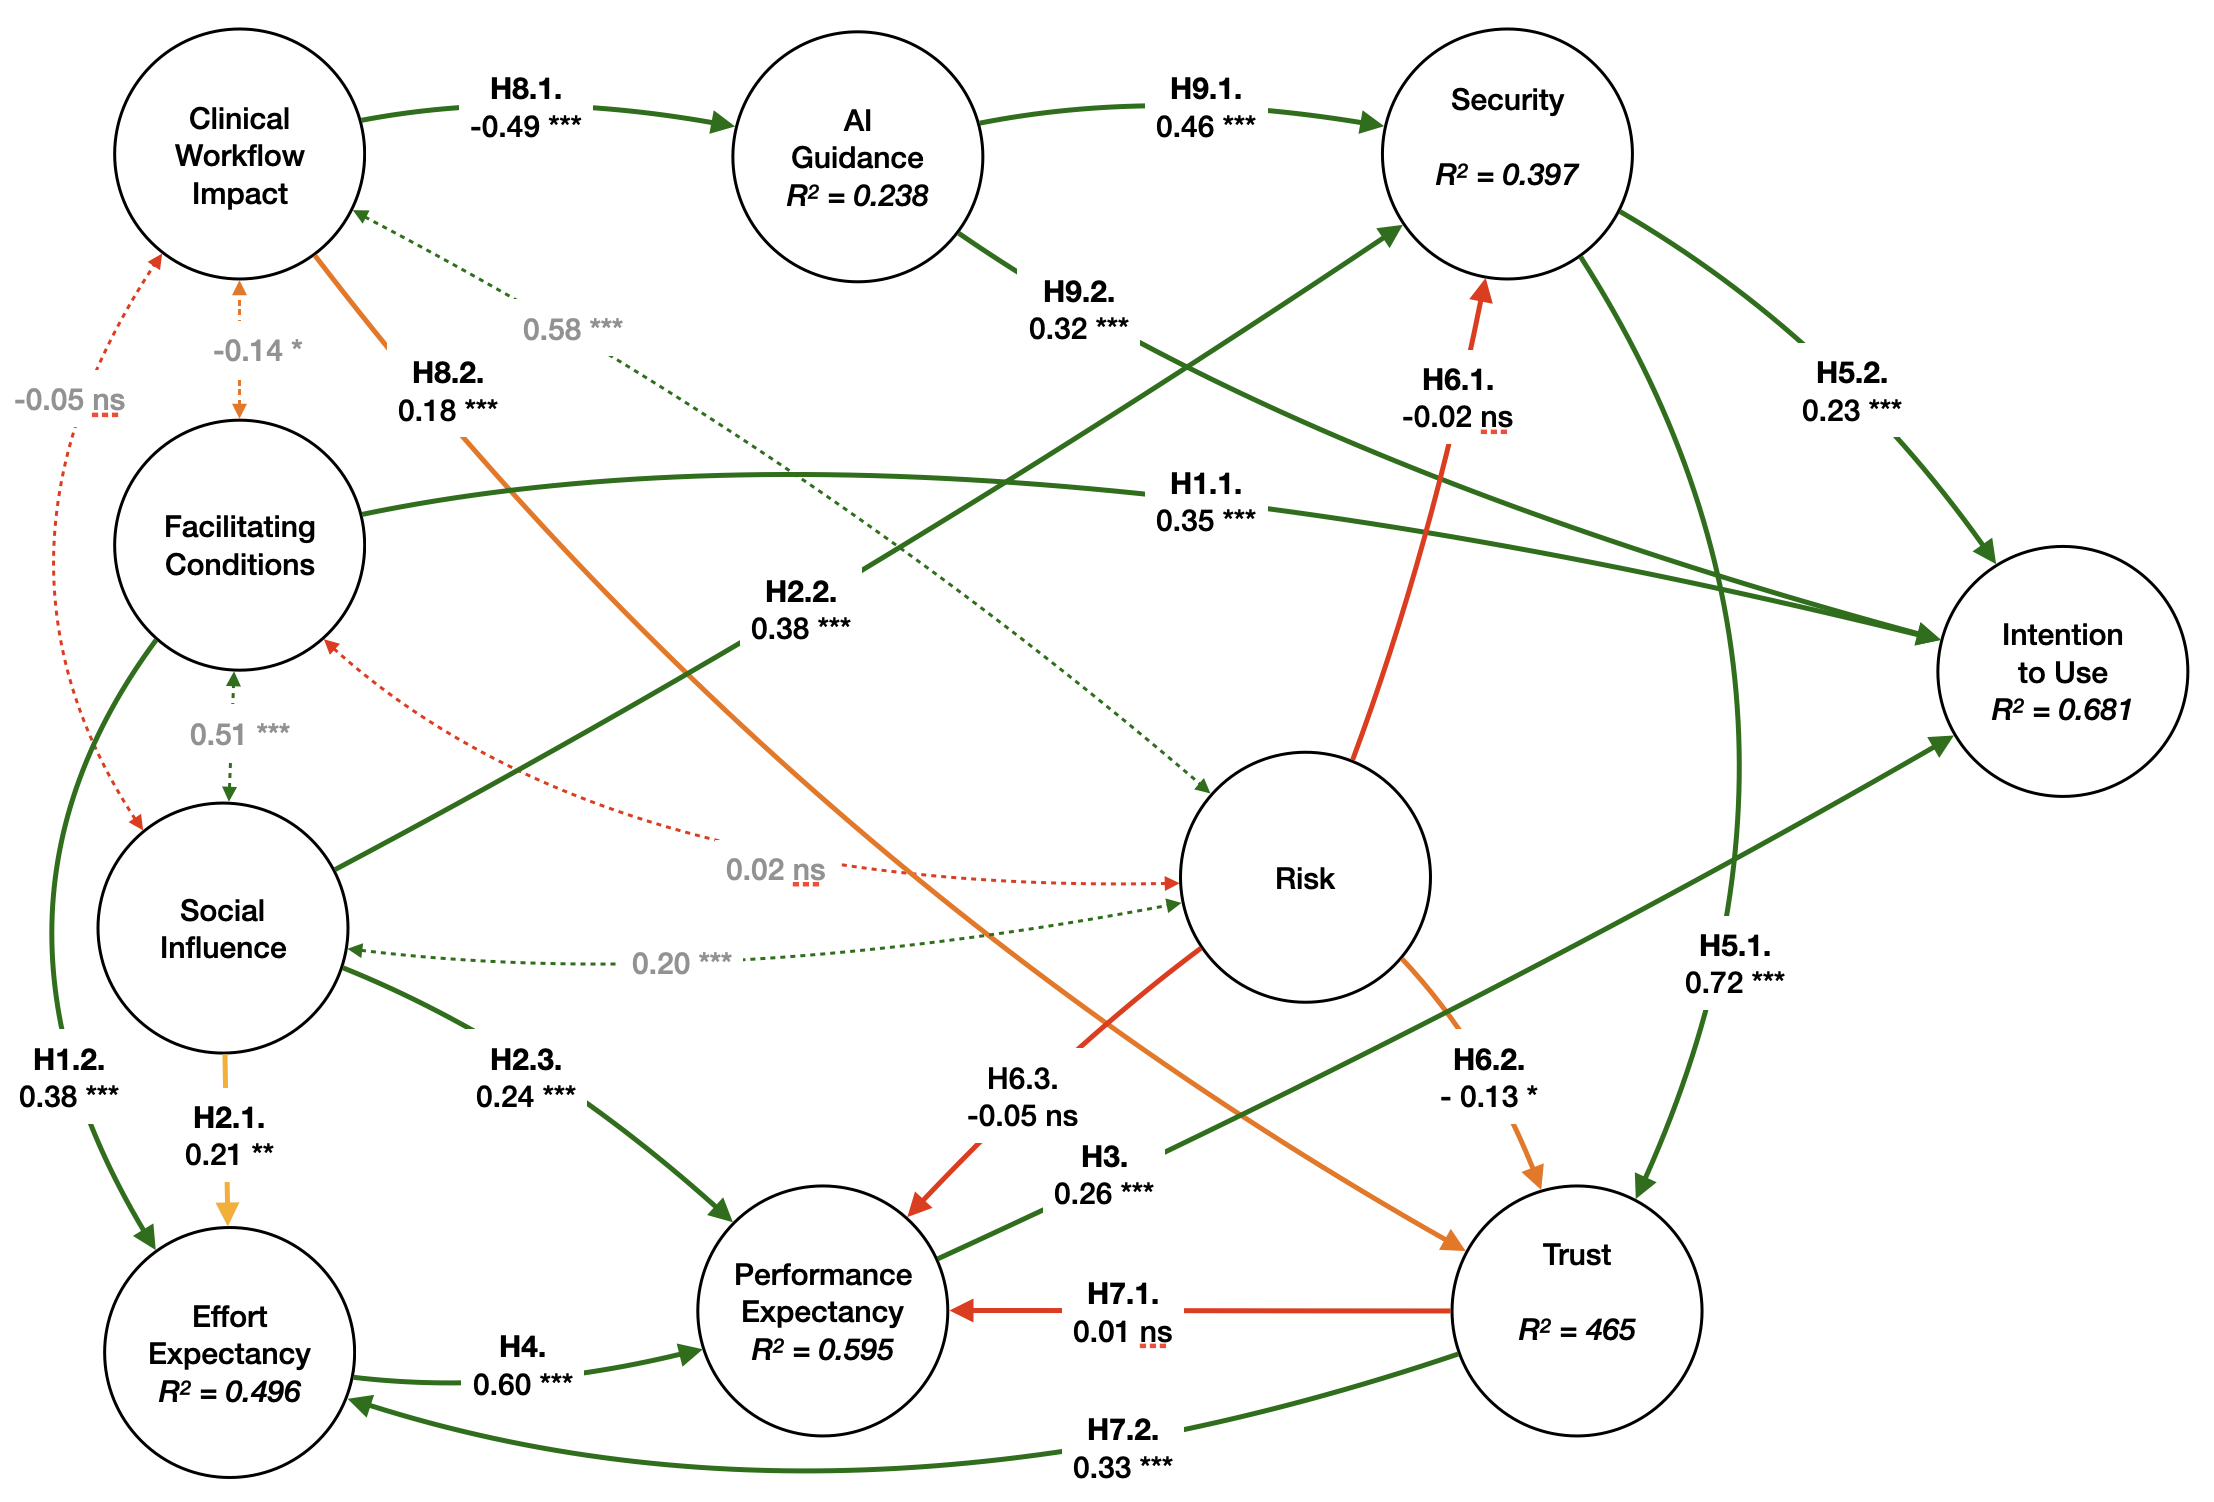
\includegraphics[width=0.985\linewidth]{fig074}
\caption{Detailed results of the research model. For beta results, the significance values are: in green for *** significant at level $\alpha = 0.01$; yellow for ** significant at $\alpha = 0.05$; orange for * significant fixed at $\alpha = 0.10$; and red for \underline{n}ot \underline{s}ignificant (ns).}
\label{fig:fig074}
\end{figure}
%%%%%%%%%%%%%%%%%%%%%%%%%%%%%%%%%%%%%%%%%%%%%%%%%%%

\textcolor{revised}{As detailed in Section~\ref{sec:chap004006002}, the design recommendations emerged from an iterative process of analyzing the empirical data in conjunction with the theoretical insights gained from our model.
Specifically, we scrutinized how clinicians' perceptions of security, risk, and trust influence their receptiveness to \ac{AI} recommendations.
This analysis was further enriched by integrating established concepts from the literature on \ac{AI} trustworthiness, bias mitigation, and the importance of explainable \ac{AI} in clinical settings.
Doing so ensured our recommendations are empirically grounded and theoretically robust, addressing critical concerns in deploying \ac{AI} in medical diagnostics.
The subsequent sections will elaborate on these recommendations, highlighting their practical implications for designing user-centric \ac{AI} tools in healthcare and how they contribute to the broader discourse on \ac{AI} adoption in clinical environments.}

\subsection{Main Findings}
\label{sec:chap004006001}

\textcolor{revised}{This section explores vital findings across factors like facilitating conditions and trust dynamics, illuminating the intricacies of clinician-\ac{AI} interactions and informing our design strategy.
Our exploration covers facilitating conditions (Section~\ref{sec:chap004006001001}), social influence (Section~\ref{sec:chap004006001002}), performance expectations (Section~\ref{sec:chap004006001003}), security (Section~\ref{sec:chap004006001004}), risk (Section~\ref{sec:chap004006001005}), trust (Section~\ref{sec:chap004006001006}), \ac{AI} guidance (Section~\ref{sec:chap004006001007}), and other factors (Section~\ref{sec:chap004006001008}), informing clinician perceptions and interactions with \ac{AI} systems.
This analysis highlights the need for a design framework that aligns with clinicians' ethos and needs, ensuring \ac{AI} tools are effective and meet their requirements.}

\subsubsection{Facilitating Factors}
\label{sec:chap004006001001}

\textcolor{revised}{Figure~\ref{fig:fig074} illustrates the key findings of our study, which significantly inform the design recommendations in Section~\ref{sec:chap004006002}.
Our analysis revealed that facilitating conditions are a strong predictor of clinicians' intention to use \ac{AI} in clinical workflows ({\bf H1.1.}), underscoring the importance of supportive environments for \ac{AI} adoption.
This finding aligns with existing literature emphasizing the role of facilitating conditions in enhancing user acceptance~\cite{Lambert2023, KHANIJAHANI2022100602}, particularly in these high-stakes domains.
Furthermore, our results demonstrate a notable link between facilitating conditions and effort expectancy ({\bf H1.2.}), suggesting that ease of use is a critical factor in clinician engagement with \ac{AI} tools.}

\subsubsection{Social Factors}
\label{sec:chap004006001002}

\textcolor{revised}{The influence of social factors was also evident, with social influence directly impacting effort expectancy ({\bf H2.1.}), perceived security ({\bf H2.2.}), and performance expectancy ({\bf H2.3.}).
This highlights the role of social dynamics when adopting \ac{AI} systems in healthcare settings.
These insights are grounded in the broader discourse on trust and bias in \ac{AI}~\cite{CHOUDHURY2022103708}, as social influence can shape clinicians' trust in \ac{AI} systems and potentially introduce biases in their adoption and use.}

\subsubsection{Performance Factors}
\label{sec:chap004006001003}

\textcolor{revised}{The study's findings underscore the significant role of performance expectancy in shaping clinicians' intention to use \ac{AI}, as evidenced by our hypothesis ({\bf H3.}), with a notable impact observed among {\it male expert} clinicians (Table~\ref{tab:tab012}).
This insight aligns with existing literature that emphasizes the importance of perceived effectiveness in technology adoption~\cite{SOLAIMANI2023101760, HSIEH2023107868}, particularly in complex clinical settings like medical imaging.
Effort expectancy's positive influence on performance expectancy ({\bf H4.}) further highlights the need for user-friendly \ac{AI} systems that can seamlessly integrate into clinical workflows, reducing the cognitive load on clinicians.}

\subsubsection{Security Factors}
\label{sec:chap004006001004}

\textcolor{revised}{Our analysis also reveals that security is a critical factor in building clinicians' trust in \ac{AI} systems ({\bf H5.1.}), influencing their attitudes and behavioral intentions ({\bf H5.2.}).
This finding is particularly relevant in healthcare, where data security and patient privacy are paramount~\cite{6038874, HLAVKA2020235}.
It suggests that design recommendations for \ac{AI} systems in medical imaging should prioritize robust security measures to foster trust among clinicians.
Furthermore, advanced security protocols protect sensitive data and boost clinicians' confidence in \ac{AI} tools~\cite{KHANIJAHANI2022100602}, promoting their acceptance and integration into clinical practice.}

\subsubsection{Risk Factors}
\label{sec:chap004006001005}

\textcolor{revised}{Additionally, perceived risk, as indicated by our hypothesis ({\bf H6.3.}), plays a pivotal role for certain clinician groups, affecting their beliefs about \ac{AI}'s performance and trust in maintaining patient privacy.
This observation is crucial for understanding the nuances of \ac{AI} adoption across different user demographics and specialties.
It points to the necessity of tailoring \ac{AI} systems to address specific concerns and biases~\cite{Topol2019, 10.1145/3290605.3300831}, ensuring that they are technically proficient and aligned with the medical field's ethical standards and privacy needs.}

\subsubsection{Trust Factors}
\label{sec:chap004006001006}

\textcolor{revised}{Our study reveals differences in trust's impact on performance expectancy ({\bf H7.1.}) and effort expectancy ({\bf H7.2.}) between {\it novice} and {\it expert} clinicians.
This highlights the need for adaptable \ac{AI} systems in healthcare, suitable for varying levels of clinician experience and trust.
Referencing the literature~\cite{gunning2017explainable, 10.1145/3411764.3445717}, we advocate for \ac{AI} systems with scalable guidance, particularly aiding novice clinicians.
These findings inform our design recommendations for personalized, context-specific \ac{AI} assistance.
Integrating \ac{XAI} principles~\cite{10.1145/2939672.2939778}, we aim to enhance transparency and reduce biases towards personalized \ac{AI} suggestions, building trust among clinicians with diverse expertise.
Therefore, adaptable and customized \ac{AI} guidance are essential characteristics for their effective adoption in various clinical settings.}

\subsubsection{Guidance Factors}
\label{sec:chap004006001007}

\textcolor{revised}{The impact of \ac{AI} guidance on security perceptions ({\bf H9.1.}) and behavioral intention ({\bf H9.2.}) varies among clinician groups, aligning with research highlighting security's importance in \ac{AI} systems~\cite{MALAMATENIOU20211192}.
Our design recommendations focus on integrating robust, adaptable security settings in diverse healthcare environments, essential for building trust and acceptance among various user demographics.
This approach, supported by literature on security's role in user trust~\cite{Amann2020}, also aligns with bias mitigation and system explainability efforts~\cite{SHIN2021102551}.
Recognizing these findings' variability, we emphasize the need for context-aware \ac{AI} solutions across different medical institutions, radiologists, and countries.}

\subsubsection{Other Factors}
\label{sec:chap004006001008}

\textcolor{revised}{While several hypotheses ({\it e.g.}, {\bf H6.1.}, {\bf H6.2.}, {\bf H8.1.}, or {\bf H8.2.}) did not find empirical support, our detailed examination in Section~\ref{chap:app002005001} of Appendix~\ref{chap:app002} delves deeper into these constructs.
This further analysis uncovers their relevance in particular contexts and for specific clinician groups, underscoring the necessity to cater to varied user needs and perceptions in \ac{AI} system design.
The findings inform our design recommendations, which emphasize the creation of \ac{AI} tools that are not just technically adept, but also resonate with the diverse expectations and requirements of different clinician demographics.}

\textcolor{revised}{The design recommendations in Section~\ref{sec:chap004006002} stem from analyzing empirical data and \ac{UTAUT}-based theoretical insights, focusing on clinicians' perceptions of security, risk, and trust in \ac{AI}.
Integrating literature on \ac{AI} trustworthiness~\cite{10.1145/3411764.3445717}, bias mitigation~\cite{10.1145/3290605.3300831}, and explainability~\cite{10.1145/2939672.2939778}, our recommendations are empirically and theoretically informed.
They emphasize enhancing facilitating conditions like comprehensive training to improve clinicians' effort expectancy and security perception.
Emphasizing transparency and explainability in \ac{AI} systems addresses biases and builds trust, aligning technology with clinical practice.
Grounded in empirical evidence and literature~\cite{CHOUDHURY2022103708}, we aim to develop effective, trustworthy \ac{AI} tools tailored to clinicians' diverse needs in medical imaging diagnosis.}

\subsection{Design Recommendations}
\label{sec:chap004006002}

\textcolor{revised}{Based on insights from Section~\ref{sec:chap004006001}, this section provides guidelines for integrating intelligent agents into medical imaging workflows, enhancing \ac{AI} as a supportive second-reader.
Trust, a crucial element for clinician engagement highlighted in literature~\cite{LIU2022107026}, is a vital focus of these guidelines.
Rooted in \ac{HCI} principles such as transparency, explainability, and workflow compatibility, the aim is to improve diagnostics and foster a synergistic clinician-\acs{AI} relationship.
Following a human-centered design approach~\cite{10.1145/3313831.3376718}, as we describe next in Chapter~\ref{chap:chap005}, these design recommendations strive to minimize cognitive load and enhance the \ac{UX} of clinicians during the interaction with intelligent agents, making \ac{AI} assistants more intuitive and user-friendly.}

\textcolor{revised}{Incorporating \ac{HCI} principles~\cite{Knisely2021}, the design recommendations advocate for adaptability, personalization, and cognitive load management in \ac{AI} systems, catering to the unique demands of clinical environments.
Usability and interpretability are pivotal for seamlessly integrating \ac{AI} tools into healthcare routines~\cite{10.1145/3411764.3445385}.
These principles ensure that \ac{AI} solutions are intuitive, reducing unnecessary cognitive burden and fostering an environment where clinicians and \ac{AI} systems work in tandem.
For a comprehensive overview of these design considerations, consult Section~\ref{chap:app002005002} in Appendix~\ref{chap:app002}.}

\vspace{1.50mm}

\noindent
\textcolor{revised}{Our design recommendations, grounded in empirical data and theoretical insights, include:}

\vspace{0.50mm}

\begin{enumerate}
\item \textcolor{revised}{Intelligent agents should clearly communicate the implications of \ac{AI} guidance on clinical workflow~\cite{MALAMATENIOU20211192}, offering clinicians control over decisions;}
\item \textcolor{revised}{An \ac{AI} systems must adapt communication to clinicians' demographic characteristics~\cite{Alowais2023}, including gender, age, and country development categories, to ensure effective and personalized interaction;}
\item \textcolor{revised}{An \ac{AI} systems should account for the variability in medical cases~\cite{10.1145/3313831.3376506}, tailoring their approach to individual conditions and diverse \ac{AI} techniques;}
\item \textcolor{revised}{Designers and developers should enhance the ease of use (usability) and usefulness (functionality) of \ac{AI} systems to improve perceived security, perceived risk, and trust of clinicians~\cite{OPRESCU202253}.}
\end{enumerate}

\textcolor{revised}{These recommendations, informed by our study, focus on providing informative \ac{AI} guidance, personalizing communication, considering case variability, and enhancing usability and functionality.
They are designed to facilitate the effective integration of \ac{AI} technology in medical imaging's clinical workflow.
Additionally, they aim to bridge the gap between technological capabilities and clinical needs, ensuring that \ac{AI} tools are advanced and intuitively align with clinicians' daily practices.
The recommendations seek to improve diagnostic accuracy and efficiency by addressing these critical areas, ultimately improving patient outcomes.
For more detailed design considerations, please see Section~\ref{chap:app002005002} of Appendix~\ref{chap:app002}.}

\section{Boundaries}
\label{sec:chap004007}

Despite its contributions, the study has some boundaries, which provide fruitful avenues for further research.
Several of these boundaries affect the scope of our results.
Although we had a significant sample of global nationalities, there is still a bias for the small sample size (Table~\ref{tab:tab008}) of specific nationalities.
To understand the effect of this bias, we analyzed the moderator effect of country development categories in our model, which showed the same evidence of invariant measure compared to other moderators (gender, age, etc.).
However, we did not record race and ethnicity differences in our sample.
Previous works show a significant impact of cultural diversity on social influence, usefulness, and behavior intention~\cite{Belanche2019, info:doi/10.2196/27122}.

Another limitation of our study is that it involved clinicians mainly related to radiology.
Given the focus of our study, {\it i.e.}, the medical imaging field, our sample could be biased.
The effect of such characteristics limits the generalizability of this research, since the sample employed in this study could express different perceptions towards \ac{AI} systems compared to other clinical expertise.
However, the experimental design helps reduce the impact of the \ac{CMB}, which we employed in this study, particularly for the new \ac{AI} constructs.
Moreover, by combining the survey with outcome variables measured separately and more objectively ({\it e.g.}, frequency of usage/reporting), we are revealing valid results less prone to measurement and method bias.

Despite the above boundaries, this study fosters the community's understanding of the intention to use \ac{AI} systems in the clinical workflow. Specifically for the associated constructs of security, risk, and trust concerns on \ac{AI} systems.
Finally, we provide valuable design guidelines and recommendations for delivering \ac{AI} systems with these concerns to different user groups.

\section{Conclusion}
\label{sec:chap004008}

In this chapter, we conducted a comprehensive investigation into the acceptance and adoption of \ac{AI} systems in the clinical workflow of medical imaging diagnosis.
The study focused on understanding the role of security, risk, and trust in influencing clinicians' acceptance of \ac{AI}-based assistance.
Through empirical testing, we confirmed that trust plays a critical role in shaping user acceptance, mediating the effects of \ac{AI}-specific aspects of user behavior.
Additionally, clinicians' demographic characteristics, such as gender, age, and educational background, moderate the relationship between these factors and their intention to use \ac{AI} systems.
These findings underscore the importance of considering clinicians' specific needs and characteristics when developing intelligent agents for medical imaging diagnosis.
Integrating \ac{HCI} principles into developing \ac{AI}-based assistance to create user-friendly and effective systems, enhancing clinical workflows and improving patient outcomes.

The research conducted in this chapter provides valuable insights and implications for the design, development, and deployment of \ac{AI}-based assistance in healthcare.
The study highlights the significance of trust, addresses security, and risk concerns, while offering practical guidelines for integrating \ac{AI} systems into the clinical workflow, building upon the design interventions discussed in Chapter~\ref{chap:chap005}.
Chapter~\ref{chap:chap006} further explores the importance of tailoring communication methods to address the specific needs of different user groups, enhancing clinicians' engagement and acceptance of \ac{AI} technology.
This comprehensive approach, encompassing adoption studies (Chapter~\ref{chap:chap004}), design interventions (Chapter~\ref{chap:chap005}), and tailored adaptive communication (Chapter~\ref{chap:chap006}), promotes the successful acceptance and integration of \ac{AI} systems in healthcare settings.
The final remarks can be found in Section~\ref{chap:app002006} of Appendix~\ref{chap:app002}, providing a more comprehensive and in-depth perspective on the summarized conclusions.
% If Printing on DOUBLE SIDED pages, the second page should be white.
% Otherwise, comment the following command:
\cleardoublepage
%
% Chapter 5
% #############################################################################
% This is Chapter 5
% !TEX root = main.tex
% #############################################################################
% Change the Name of the Chapter i the following line
\fancychapter{Assessment \& Implications}
\clearpage
% The following line allows to ref this chapter
\label{chap:chap005}

\vspace{0.05mm}

\noindent
{\it Chapter~\ref{chap:chap005} was published in two journals, ranked Q1 in 2021 and 2022, respectively:}

\vspace{0.05mm}

\begin{itemize}
\item {\bf Francisco Maria Calisto}, Carlos Santiago, Nuno J. Nunes, Jacinto C. Nascimento, Introduction of Human-Centric AI Assistant to Aid Radiologists for Multimodal Breast Image Classification, International Journal of Human-Computer Studies, Volume 150, 2021, 102607, ISSN 1071-5819. DOI: \href{https://doi.org/10.1016/j.ijhcs.2021.102607}{doi.org/10.1016/j.ijhcs.2021.102607}
\item {\bf Francisco Maria Calisto}, Carlos Santiago, Nuno J. Nunes, Jacinto C. Nascimento, BreastScreening-AI: Evaluating Medical Intelligent Agents for Human-AI Interactions, Artificial Intelligence in Medicine, Volume 127, 2022, 102285, ISSN 0933-3657, DOI: \href{https://doi.org/10.1016/j.artmed.2022.102285}{doi.org/10.1016/j.artmed.2022.102285}
\end{itemize}

For this thesis, the main goal is to understand how the implemented \ac{DL} methods (Appendix~\ref{chap:app004}) can be integrated within an intelligent agent.
Moreover, it is essential to understand how the intelligent agent(s) can better communicate with clinicians as a second reader.
In this chapter, we take an \ac{HCI} perspective on the implications of \ac{AI} techniques~\cite{CALISTO2022102285} across the assessment of medical imaging~\cite{CALISTO2021102607}, focusing on workflow efficiency and quality, preventing medical errors and variability of diagnosis in breast cancer.

\section{Motivation}
\label{sec:chap005001}

The combination of \ac{AI} and medical imaging, known as ``radiomics''~\cite{Lambin2017}, has the potential to revolutionize radiology by automating the analysis of large amounts of data and extracting meaningful features to support diagnosis and clinical decision-making~\cite{Ruddle:2016:DEI:2872314.2834117}.
However, while modern assistant technologies such as \ac{DL} methods show promising accuracy (Section~\ref{sec:app003001}), the probabilistic nature of their algorithms can lead to mistrust and abandonment by clinicians who do not expect their clinical systems to behave inconsistently and imperfectly~\cite{Kocielnik:2019:YAI:3290605.3300641}.
Therefore, evaluating the acceptance and usability of \ac{AI}-based clinical systems was crucial to ensure successful adoption (Chapter~\ref{chap:chap004}) in real-world clinical setups.

Deficiencies in experimental and analytic designs have been identified in some studies~\cite{Sultanum:2018:MTP:3173574.3173996}.
However, these studies fail to include a more holistic understanding of the clinical context.
Another important consideration on using \ac{AI} in real-world clinical settings is the trust and usability of interactive assistance techniques~\cite{Cadario2021}.
While much work has focused on improving the accuracy of \ac{AI} algorithms, comparatively less work has been done to improve trust and usability~\cite{CALISTO2021102607}.
Thus, our research aims to answer high-level questions about how radiologists accept and interact with AI-assisted systems, how receptive they are to their introduction, and how they are affected by \ac{AI} assistance in different clinical contexts~\cite{CALISTO2022102285, CALISTO2021102607}.
For that, we propose an \ac{AI}-assisted approach, which integrates \ac{DL} techniques with a real clinical workflow for a multimodal medical imaging diagnosis~\cite{10.1145/3399715.3399744}.
Our proposed approach aims to improve diagnosis accuracy and reduce cognitive workload.
We also consider the importance of providing reasons for \ac{AI} recommendations to foster model transparency and user trust.

\subsection{Contributions}
\label{sec:chap005001001}

We created our proposed technique, based on the following contributions:
(1) exploring the power of explanations and the users' need for control on the introduction of \ac{AI} methods among medical imaging diagnosis; and
(2) studying the \ac{AI} impact on the radiologists' {\it behaviour} in professional practice.
We did that to achieve higher user expectations of the system capabilities, addressing potential gaps.
Although efforts have been dedicated to enhancing the precision of \ac{AI} algorithms, there has been relatively less emphasis on enhancing trust and usability of interactive assistance techniques.
Therefore, we ask several high-level questions, namely:
i) how they {\it accept} and {\it interact} with these systems;
ii) how {\it receptive} are the clinicians to the introduction of \ac{AI} assistance;
iii) how clinicians are {\it affected} by the \ac{AI} assistance in different clinical contexts.
This chapter contributes broadly to the literature in \ac{HCI} and \ac{AI} by examining what radiologists need when using \ac{AI}-powered image diagnostic, the practices they adopt while using these tools, and how they affect end-user attitudes towards the underlying \ac{AI} algorithms.

\subsection{Research Questions}
\label{sec:chap005001002}

A vital component of this dissertation thesis was to access many clinical settings and radiologists.
In this thesis, the work has established the foundations of its research via a human-centered design process and following the literature guidelines (Section~\ref{sec:app003002} of Appendix~\ref{chap:app003}) for \ac{HAII}~\cite{10.1145/3313831.3376718, 10.1145/3290605.3300233, 10.1145/3290605.3300234, Kocielnik:2019:YAI:3290605.3300641}, including:
i) findings from a user study in nine clinical institutions, encompassing {\it in-situ} observations and interviews, as well as grounded by related work; which informed
ii) a list of design recommendations for medical imaging systems, including temporal awareness, image processing, multimodality, trust, acceptance, and usage; leading to
iii) findings from an evaluation study of {\it BreastScreening-AI}, a proof-of-concept prototype that was developed to support the clinical translation of {\it radiomics}, validated by 45 physicians; and finally
iv) evidence from the impact of multimodality and \ac{AI}-assisted strategy in diagnosing breast cancer patients and severity classification of lesions.

\vspace{2.50mm}

\noindent
By focusing on the integration of multimodality and \ac{AI} techniques in {\it BreastScreening-AI} and clinical workflows, we formulated the following three research questions:

\vspace{0.05mm}

%%%%%%%%%%%%%%%%%%%%%%%%%%%%%%%%%%%%%%%%%%%%%%%%%%
\begin{enumerate}
\item {\bf RQ5.1.} What is the impact on clinicians' satisfaction and acceptance of \ac{AI} assistance with applied design interventions in radiology?
\item {\bf RQ5.2.} How can we improve clinicians' understanding and trust in \ac{AI} recommendations using design techniques to increase the explainability power of the system?
\item {\bf RQ5.3.} What is the impact of \ac{AI} assistance on the medical workflow, including accuracy, time performance, and variability in patient classification?
\end{enumerate}
%%%%%%%%%%%%%%%%%%%%%%%%%%%%%%%%%%%%%%%%%%%%%%%%%%

\section{Background}
\label{sec:chap005002}

In this section, two areas motivate our research work:
a) related works designing autonomous systems ({\it e.g.}, {\it radiomics}, \acp{CADe}, \acp{CADx}, \acp{CDSSe}) for the clinical workflow, while providing an assisted medical imaging analysis; and
b) the theories of \ac{HAII} collaboration while covering users' expectations and potential gaps.
The section begins by outlining the role of design for the clinical workflow and how it is currently handled in various steps of the \ac{DL} pipeline and {\it radiomics} stages (Figure~\ref{fig:fig027}, Section~\ref{sec:app004001} of Chapter~\ref{chap:app004}), including image segmentation, feature extraction, and image classification.
Then, the section introduces existing \ac{HAII} techniques for integrating intelligent agents into the framework.

\subsection{Clinical Workflow Design}
\label{sec:chap005002001}

In modern healthcare, medical images play a crucial role in supporting decision-making for diagnosis, predictions, and treatment planning~\cite{liang2019deep}.
Accurate lesion detection and segmentation are often mandatory for image analysis and {\it radiomics}, where numerous methods have been proposed to automatically perform these tasks~\cite{litjens2017survey}.
In the field of breast cancer, medical imaging systems allow clinicians to diagnose several modalities from the retrieval of medical imaging data~\cite{seifabadi2019correlation}.
To enhance clinical workflows, a wide range of \acp{CDSSe} are designed, including those that provide potential information for medical decision-making and those that make diagnostic decisions~\cite{10.1145/3290605.3300234, GU2020101858}.
However, experts may resist using a system if it does not capture the nuances of their mental models or provides relevant context~\cite{10.1145/2858036.2858373}.
Conversely, clinicians are known to resist changes and new tools~\cite{10.1145/3132272.3134111}, an issue that has an impact in their workflow.
In our research, we take a human-centered approach to understanding various design aspects and expectations of a medical imaging \ac{CDSSe} that is integrated into a real radiology workflow.
To accomplish this, we use methods such as bringing focus groups, workshops, observations, and interviews from the literature~\cite{Lim:2019:DDI:3319806.3301427} into our user research activities (Section~\ref{sec:chap005003001}).
By doing so, we aim to understand better how the system can be designed to meet the needs and expectations of its users (Section~\ref{sec:app003004007} of Appendix~\ref{chap:app003}), including radiologists and other medical professionals who work with the system on a regular basis.
In particular, our work demonstrates how an interactive \ac{AI} can directly address the above-mentioned challenges during medical imaging diagnosis.

The field of \ac{AI} is providing several \ac{DL} work models to assist clinical practitioners with appropriate knowledge~\cite{9540298, 9730804}.
However, the literature does not typically address the effectiveness of clinical \ac{AI} solutions from the perspective of human users~\cite{CALISTO2021102607}.
The work of Xie et al.~\cite{10.1145/3313831.3376807} has established the importance of providing reasons for the design of \ac{AI} recommendations to foster model transparency and user trust within these clinical workflows.
This work stressed that clinical systems should be designed based on the user needs of clinical practitioners, but the speculative evaluation of their system design does not provide much evidence of its integration into a real clinical workflow.

In another direction, Schaekermann et al.~\cite{10.1145/3313831.3376506} argue that explanations for clinical cases can be leveraged by \ac{AI} assistants to support medical reasoning.
Although similar to what we are doing in this work, these authors are not using real \ac{AI} outputs.
Instead, they are simulating hypothetical \ac{AI} scenarios and agent behaviors, manually generated by clinicians.
However, their work highlights the importance of explainability and interpretability of \ac{AI} models in the medical domain.
Concerning explainability and interpretability, two approaches are currently proposed: \ac{XAI} and Intelligibility~\cite{gunning2017explainable}.
\ac{XAI} and Intelligibility must take into account the fact that diverse data may contribute to a relevant result~\cite{10.1145/3411764.3445736, Bharadhwaj:2019:ERS:3308557.3308699}.
The work done by Holzinger et al.~\cite{holzinger2018current} addresses this need, namely {\it how} and {\it why} a machine has reached a given decision~\cite{shah2019artificial}.
Moreover, transparent algorithms could appropriately enhance the trust of clinicians in future \acp{HAII}~\cite{Dominguez:2019:EEA:3301275.3302274, Weisz:2019:BTS:3301275.3302290}.
Our work contributes novel perspectives on the system design and integration of a real \ac{DL} model for clinical assessments (Section~\ref{sec:app003003005} of Appendix~\ref{chap:app003}).

\subsection{Human-AI Interaction}
\label{sec:chap005002002}

Recent advances in medical technologies have driven research in \ac{HAII} across the clinical domain, where \ac{HAII} incorporates human feedback in the model training process to create better \ac{ML} models~\cite{10.1145/3411764.3445717, 10.1145/3411764.3445562}.
The \ac{iML} topic adds human expertise to \ac{AI}/\ac{ML} processes, allowing for re-enactment and retracing of results on demand, and requires new \ac{HITL} interfaces for \ac{XAI}~\cite{CALISTO2021102607}.
While much of the previous work in \ac{HAII} has employed handcrafted features, leveraging the rich image data features automatically learned from \ac{DL} algorithms can improve clinical recommendations and clinical decision-making~\cite{holzinger2019interactive}.
Guidelines for designing \ac{HAII} systems have been provided (Section~\ref{sec:app003002}), which can help to address issues of transparency, trust, and accountability.
More precisely, the work of Amershi et al.~\cite{10.1145/3290605.3300233} is providing a set of design guidelines to evaluate the quality of explanations.
Therefore, incorporating \ac{HAII} in medical imaging diagnosis can lead to the development of more accurate and reliable \ac{AI} systems that can enhance the workflow of medical professionals.

The use of \ac{AI} in diagnosis requires addressing two key issues:
(1) trust, transparency, and accountability of the agent~\cite{10.1145/3290605.3300233}; and
(2) the user's ability to understand and predict agent behavior through explainability and intelligibility~\cite{gunning2017explainable}.
In this context, expectation theories~\cite{Kocielnik:2019:YAI:3290605.3300641} suggest that user satisfaction and system adoption are tied to the gap between initial expectations and actual clinical experience.
Specifically, Quinn et al.~\cite{QUINN2022102158} are stating that expecting more than the system can deliver will decrease user satisfaction and lead to the rejection of the system.
Misaligned \ac{AI} recommendations can cause contention.
To mitigate the effects of misaligned \ac{AI} recommendations, strategies like giving users control over final diagnostic decisions can improve user expectations and satisfaction, especially when \ac{AI} falls short.
We aim to ensure that the abilities of our intelligent agent are correctly understood~\cite{CALISTO2021102607}, while studying its impact on radiologists' behavior.
These insights are helping us to address potential gaps and ensure that users have accurate expectations of what the intelligent agent is capable of.

\section{Design Keys}
\label{sec:chap005003}

The process that leads to the design of the {\it BreastScreening-AI} prototype~\cite{CALISTO2022102285} included a holistic understanding across the context of {\it radiomics} in breast cancer (Section~\ref{sec:chap002006}).
Herein, the developed study was specifically interested in using several modalities and intelligent agents to detect and classify lesions (Section~\ref{sec:chap002004}).
Quantitative and qualitative studies were conducted in nine health institutions to understand the medical procedures (Section~\ref{sec:chap002005}) surrounding {\it radiomics} in breast cancer (Section~\ref{sec:chap002002}), including the classifications of the lesion severity (Section~\ref{sec:chap002003}) using the \ac{BI-RADS} score.
At this point, impressions were taken regarding the efficiency of clinicians, and their recommendations based on their experience for improvements of the patient {\it examination} (Section~\ref{sec:app001005001} of Appendix~\ref{chap:app001}).
Several studies demonstrated that radiologist fatigue levels and performance are related to environmental factors such as the number of \acp{FP} and \acp{FN}~\cite{waite2017tired}.
That said, the study started by analyzing the potential enhancement that an \ac{AI}-assisted diagnosis could take in the \ac{RRR}.
To better understand the clinical procedures (Section~\ref{sec:app001005}) of the \ac{RRR} workflow (Section~\ref{sec:chap002005}), we implemented several design activities with users (Section~\ref{sec:chap005003001}) to acknowledge the insights and challenges of such workplace (Section~\ref{sec:chap005003002}), as well as to inform further the design of the {\it BreastScreening-AI} prototype (Section~\ref{sec:chap005003003}).

\subsection{Design Activities}
\label{sec:chap005003001}

In this thesis, all clinicians were actively involved in the design of this medical imaging solution.
To generate clinician's empathy and involvement, several design activities from participatory design were preliminarily used~\cite{10.1145/3308558.3314123}.
Under this thesis, the following design activities consist of three aspects: (a) {\it insight}; (b) {\it ideation}; and (c) {\it implementation}.
The proposed design activities are a practical, repeatable process along with clinicians by applying a human-centered approach to achieve an optimal solution for the first requirements of the intelligent agents (Section~\ref{sec:chap005003003005}).

Interviews and observations are helpful to obtain a synthesized {\it insight} in the clinical workflow (Section~\ref{sec:chap002005}).
As design activity according to this aspect, this work went through several observations and interviews at nine clinical institutions.
From those activities, information was extracted regarding, not only, workflow (Section~\ref{sec:chap002005}), but also, clinical characteristics of participants (Section~\ref{sec:chap005005001}).

For {\it ideation}, the goal is to find novel solutions around user needs and requirements.
In terms of design activities, this work promotes several brainstorming techniques.
Those techniques are such as workshops (Section \ref{sec:chap005003003001}), focus groups (Section~\ref{sec:chap005003003002}) and affinity diagrams (Section~\ref{sec:chap005003003003}).
Affinity diagramming~\cite{harrington2016affinity} has been used in this study to organize the acquired large sets of ideas into essential data needs for the workflow (Section~\ref{sec:chap005003003004}).
In this thesis, the methods are used to organize the findings and to sort design ideas into {\it ideation} of a focus group during several workshops.
These techniques will be further detailed and discussed (Section~\ref{sec:chap005003003}).

Finally, the {\it implementation} is promoted as a way of developing the first prototyping requirements (Section~\ref{sec:chap005003003005} of Appendix~\ref{chap:app003}).
The successful {\it implementation} was quickly recognized and would rely on a bare minimum number of requirements (Section~\ref{sec:app003003003}).
Short iterations enabled us to take advantage of these design activities for properly prototyping and testing the optimal solution with clinicians.

\subsection{Insights and Challenges}
\label{sec:chap005003002}

Interviews and observations are aligned with previous research on clinician-driven diagnostic {\it tasks}~\cite{Sultanum:2018:MTP:3173574.3173996}, informing our clinical procedures (Appendix~\ref{chap:app001}).
From the research {\it insights}, the following main challenges were identified:
i) how can we design for the heterogeneous visualization nature of large imaging numbers and file sizes; and
ii) how the introduction of intelligent agents can improve patient classification.
From the  observations and interviews, it was clear that clinicians observe only a fraction of the \ac{MRI} volumes (Section~\ref{sec:app001005002} of Appendix~\ref{chap:app001}).
Also, the imaging volumes inspected are different depending on the practices of each clinical institution \textcolor{revised}{(Figure~\ref{fig:fig018})}.
For instance, it was observed that in \acs{HFF} only the \acs{DCE-MRI} at the second time instant is considered, while in \acs{IPOL} only the third time instant of imaging volume is used for diagnosis.
Consequently, the \ac{UI} should reflect the specific institution, as it will be detailed in Section~\ref{sec:chap005004002}.

%%%%%%%%%%%%%%%%%%%%%%%%%%%%%%%%%%%%%%%%%%%%%%%%%%%
\begin{figure}[ht]
\centering
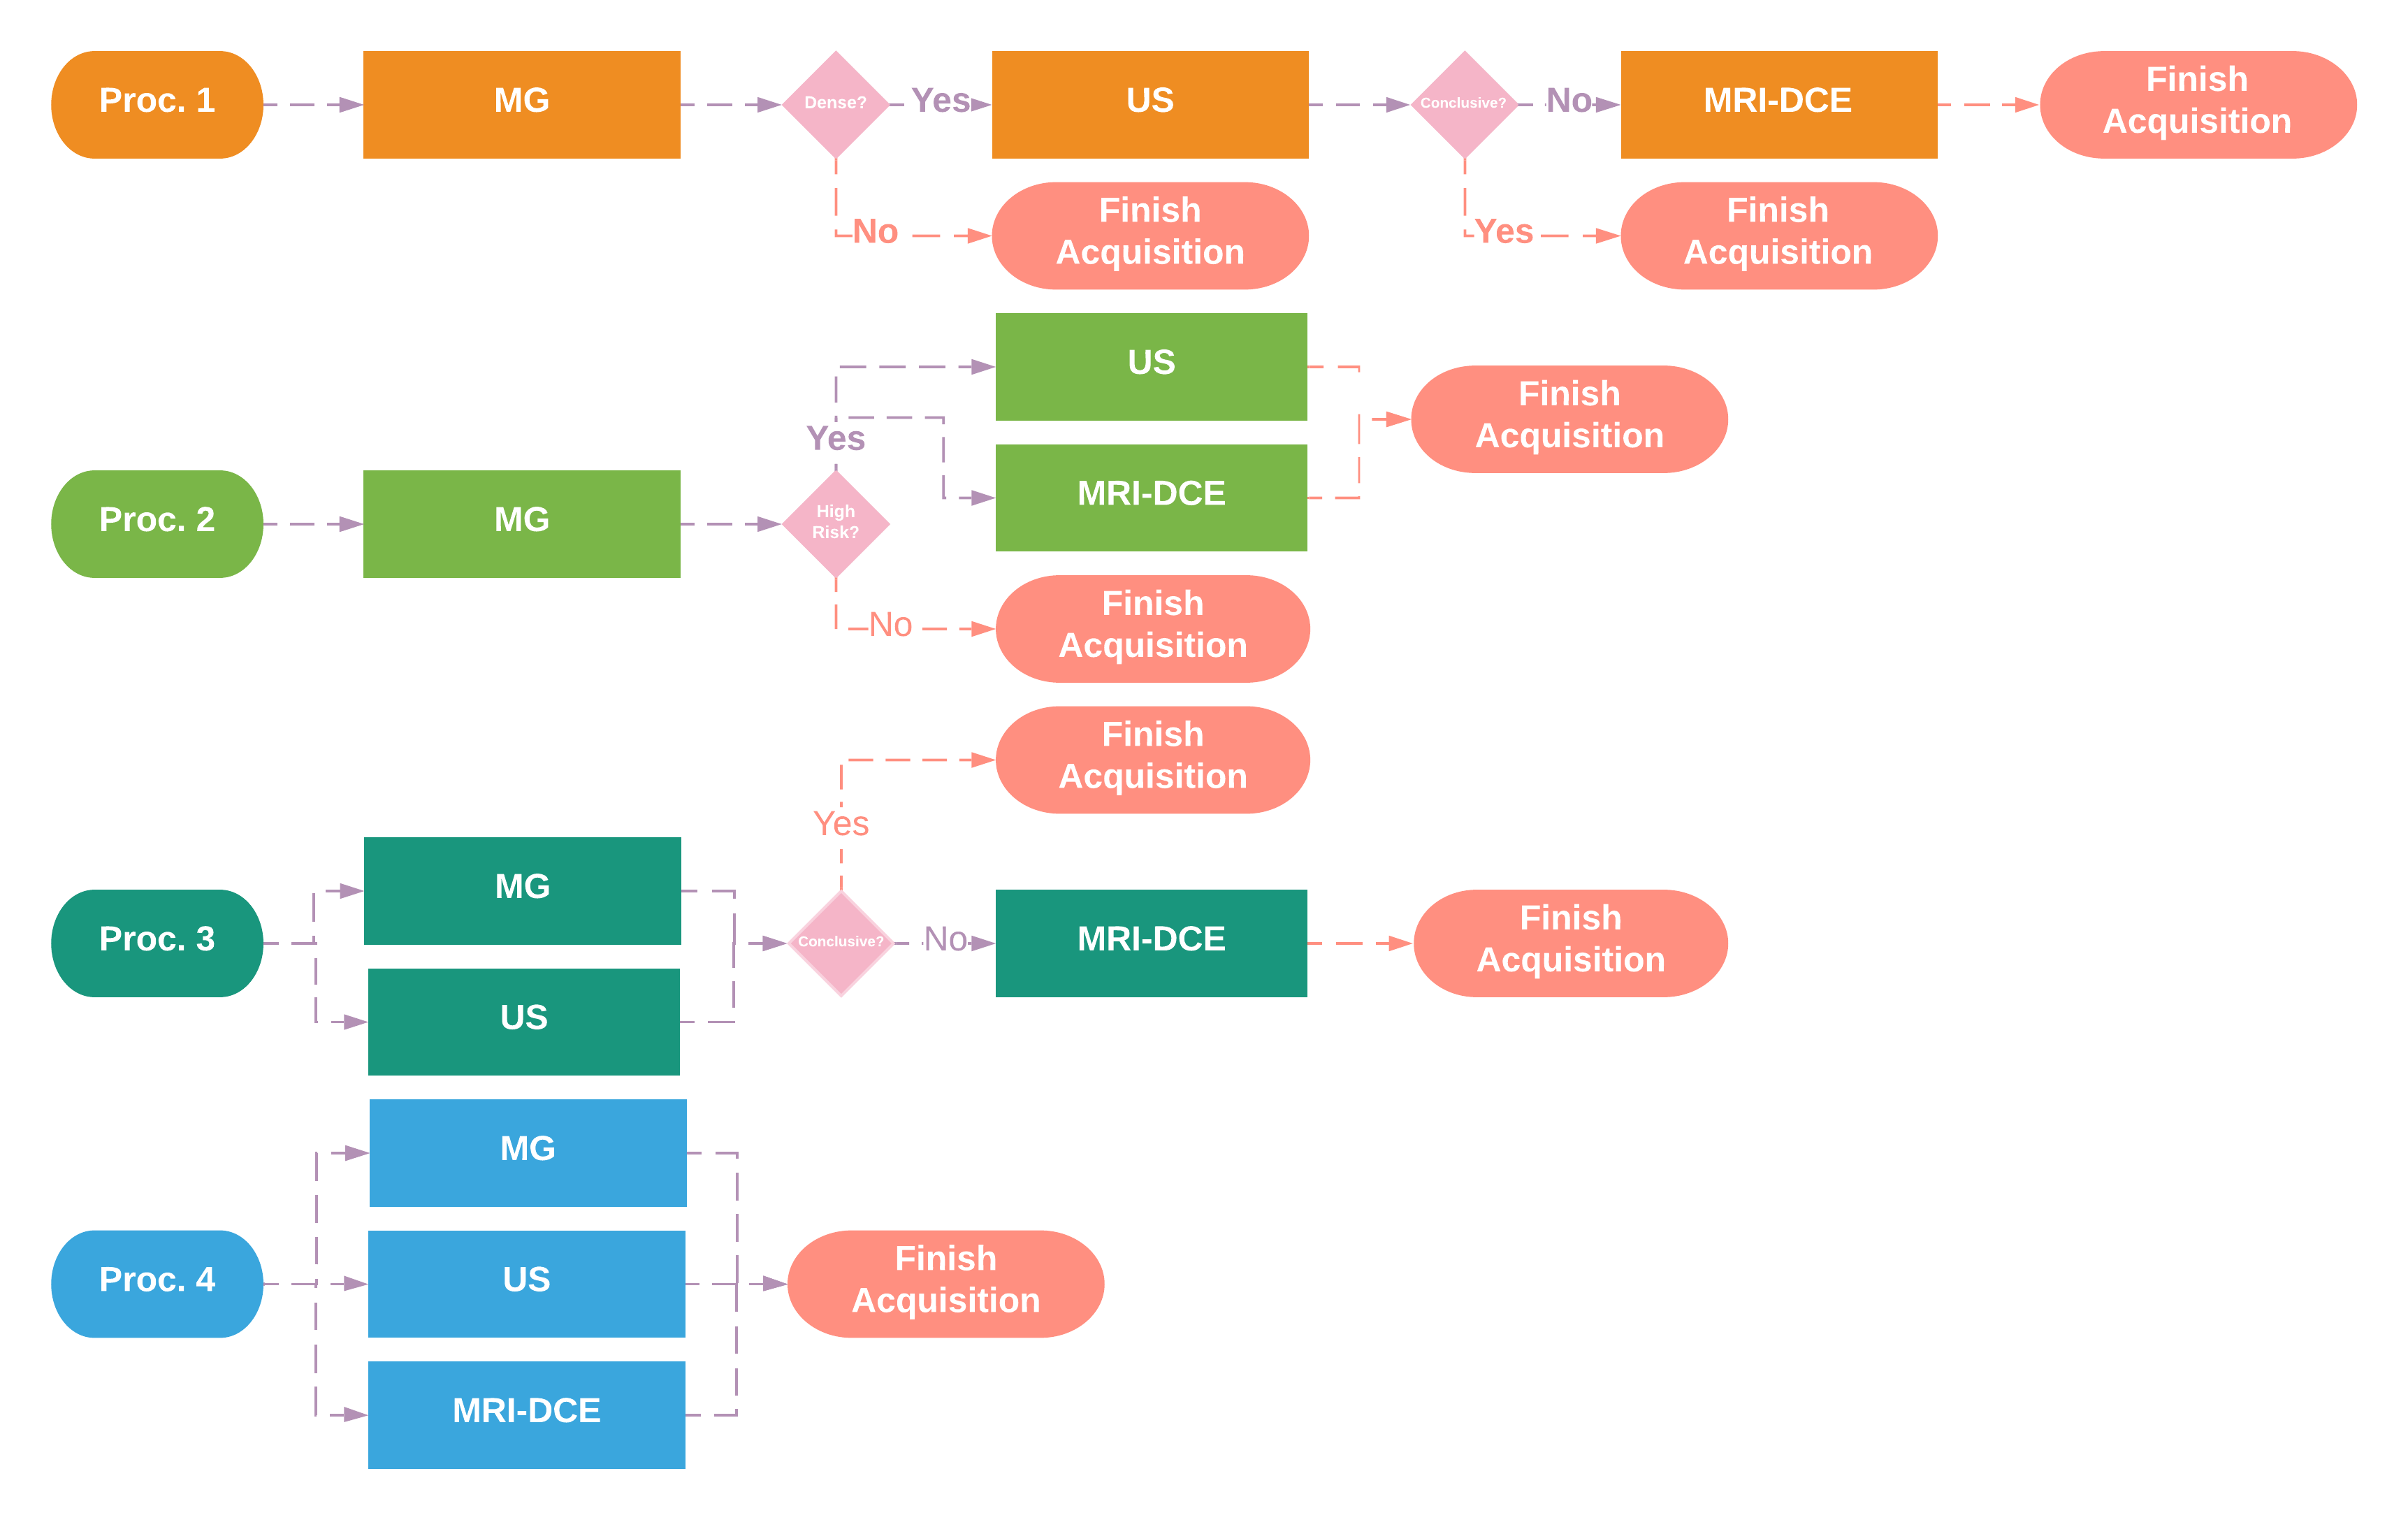
\includegraphics[width=\columnwidth]{images/fig018}
\caption{Workflow of the radiology reading room is commonly adopted in clinical institutions using several image acquisition strategies. Screening modalities ({\it e.g.}, US, MRI, etc.) constitute important complementary information for a reliable diagnosis.}
\label{fig:fig018}
\end{figure}
%%%%%%%%%%%%%%%%%%%%%%%%%%%%%%%%%%%%%%%%%%%%%%%%%%%

Related to the requirements of {\it radiomics}, the second challenge involves the generation of \ac{GT} data.
This is twofold, namely,
(i) for visualization issues, when the radiologist can inspect the delineation provided, thus, facilitating an eventual second reading of the exam, also
(ii) it constitutes valuable information for training \acp{DNN} with (semi)supervised learning procedures, as mentioned above (Section~\ref{sec:chap002006}).
This comprises the localization/delineation of anatomical microcalcification and mass lesions.
In addition, it is easier to detect the lesion patterns (Section~\ref{sec:chap002004}) by comparing the breast region in different modalities.
This is particularly relevant in designing the {\it BreastScreening-AI} prototype, since the lesions in dense breasts are almost impossible to detect in \ac{MG} (in both \ac{CC} and \ac{MLO} views) -- a recognized problem leading to numerous non-diagnosed cancers -- which only manifest later in touch exams or after severe consequences on disease progression~\cite{mohamed2018deep}.

\subsection{Preliminary Design}
\label{sec:chap005003003}

\textcolor{revised}{This thesis, rooted in \ac{UCD}, integrates insights from participant interviews into our design approach.
It details the development of a medical assistant using an iterative methodology focused on clinicians' needs.
This approach aligns the solutions with healthcare professionals' requirements, leading to intuitive and effective designs for clinical use.
Our work connects \ac{AI} technology with practical application by centering on clinicians, ensuring relevance and utility in medical practice.}

\textcolor{revised}{Workshops (Section~\ref{sec:chap005003003001}) were pivotal in this process, with participants answering open-ended questions for broad insights.
Focus groups (Section~\ref{sec:chap005003003002}), involving the research team, further utilized affinity diagrams (Section~\ref{sec:chap005003003004}) for critical idea organization.
These diagrams, essential for clustering and categorizing ideas (Section~\ref{sec:chap005003003003}), aligned with \ac{UCD} principles to ensure design evolution through user feedback and collaboration.
The following sections detail this preliminary design, demonstrating adherence to \ac{UCD} methodologies, from data collection to iterative design refinement.}

\subsubsection{Clinical Workshops}
\label{sec:chap005003003001}

\textcolor{revised}{The first step of our design activities involved exploring the {\it workflow} practices and routines of clinicians.
This process began with sending out invitations to various medical institutions and organizing at least one workshop per institution.
Participants, detailed in Section~\ref{sec:chap005005001}, were volunteers who were grouped into different sessions.
The research team dedicated at least one day to each institution for these workshops.
Specifically, the \acs{HFF} institution required four workshop sessions due to its larger clinician population, posing scheduling challenges.
\acs{IPOL} and \acs{HB} institutions hosted two sessions.
For the remaining institutions, one workshop session was sufficient.
In total, 45 healthcare professionals, including Radiologists, Oncologists, and Surgeons, along with six members of the {\it BreastScreening} research team (specializing in \acs{HCI} and \acs{AI}), participated in these workshops.}

\textcolor{revised}{The decision to conduct workshops, rather than shadowing clinicians, was influenced by ethical and privacy considerations~\cite{10.1145/3449199}.
Our established protocol with \acs{HFF} was meticulously designed to encompass specific patients within our dataset, ensuring they are under ethical approval from the hospital.
However, this protocol did not encompass patients outside the protocol.
Consequently, shadowing clinicians in their routine practice would have risked inadvertent exposure of the non-anonymized patients inside this institution's \acs{RRR}, thereby contravening established ethical and privacy norms.
In light of this, workshops emerged as a more ethically sound alternative.
They enabled us to gather valuable insights while maintaining the privacy of all patients, particularly those who were not directly informed about or involved in our research activities.
This approach not only adhered to ethical standards but also ensured the integrity of our research process in the sensitive clinical environment.}

\textcolor{revised}{These workshops, integral to the {\it BreastScreening} research, involved group-based brainstorming sessions about clinical practices and routines.
The majority of these practices were meticulously recorded and subsequently transcribed digitally.
During these sessions, we employed the affinity diagramming\footnotemark[6] technique (Section~\ref{sec:chap005003003003}) to organize and analyze the data systematically.
This participatory approach was deliberately chosen to ensure that the design of our novel intelligent agent was informed by direct feedback and real-world needs, facilitating its seamless integration into clinical settings.}

%%%%%%%%%%%%%%%%%%%%%%%%%%%%%%%%%%%%%%%%%%%%%%%%%%%
\footnotetext[6]{Affinity diagramming is a methodical approach for organizing and analyzing complex data sets. In our context, it was pivotal in understanding the role of technology within radiology workflows. By using affinity diagrams, we could categorize clinicians' information into coherent groups, aligning them with related ideas or topics, and enhancing our understanding of their workflow intricacies.}
%%%%%%%%%%%%%%%%%%%%%%%%%%%%%%%%%%%%%%%%%%%%%%%%%%%

\textcolor{revised}{Each workshop session lasted approximately two hours and concluded with joint sessions where each clinician group highlighted critical aspects of the clinical {\it workflow} for their institutions.
Four distinct procedures for acquiring medical images were collated at the end of these sessions (Figure \ref{fig:fig018}).
Participants actively engaged in the design activities, providing valuable inputs regarding the intelligent agent.
Utilizing the insights gathered from the workshops, a prototype was developed and subsequently evaluated during multiple sessions across the nine clinical institutions (Section~\ref{sec:chap005005003}).}

\subsubsection{Focus Groups}
\label{sec:chap005003003002}

\textcolor{revised}{After the workshops with clinicians (Section~\ref{sec:chap005003003001}), a focus group of six Researchers (\acs{MSc}, \acs{PhD}, Post-Doc students, and faculty) and six Radiologists (2 seniors; 1 middle; 2 juniors; and 1 intern) from \acs{HFF} used affinity diagrams to organize {\it workflow} practices and functionality ideas~\cite{CALISTO2021102607}.
Using these affinity diagrams was an essential aspect of our \ac{UCD} methodology, enabling the systematic identification and prioritization of functionalities.
For instance, the affinity diagrams highlighted the critical need for clinicians to {\it accept} or {\it reject} the {\it assistant}'s results.
Notably, the affinity diagrams revealed a high-priority need for a feedback mechanism to retrain the DenseNet when clinicians {\it reject} the intelligent agent's recommendation (Section~\ref{sec:app004004} of Appendix~\ref{chap:app004}).
This approach refines functionalities based on clinician input, exemplifying \ac{UCD} and ensuring the design evolves with user needs and feedback.}

% \vspace{1.00mm}

\noindent
The technique is novel and, while applying these \ac{HCI} practices, it provides twofold contributions:

\vspace{0.50mm}

%%%%%%%%%%%%%%%%%%%%%%%%%%%%%%%%%%%%%%%%%%%%%%%%%%%
\begin{enumerate}
\item Creating a new way of control on the introduction of \ac{AI} methods, via intelligent agents among medical imaging diagnosis; and
\item The inclusion of a \ac{DNN} in the \ac{UI} with the anthropomorphic characteristics of an intelligent agent, particularly, the introduction of a pre-trained DenseNet capable of providing a fast and reliable classification for humans to interpret.
To the best of our knowledge, this is the first attempt to include in the \ac{UI} feedback coming from a \ac{DNN} in breast cancer diagnosis with these characteristics.
\end{enumerate}
%%%%%%%%%%%%%%%%%%%%%%%%%%%%%%%%%%%%%%%%%%%%%%%%%%%

\vspace{0.50mm}

Another important aspect coming from these focus groups is that the \ac{MG} image modality is always present on a first stage of medical image acquisition, mainly because of its low cost.
The \ac{US} is the second most preferred modality to cross information between \ac{MG} image modality views ({\it i.e.}, \ac{CC} or \ac{MLO}).
Finally, because of the high costs ({\it e.g.}, time of acquiring the images) associated with the \ac{MRI}, clinicians said (in nine institutions only one follows the {\bf Proc. 4}, see Figure \ref{fig:fig018}) it was typically recommended only for highly risk patients.

\subsubsection{Affinity Diagrams}
\label{sec:chap005003003003}

\textcolor{revised}{The use of affinity diagrams in our study was a dynamic and interactive process (Figure~\ref{fig:fig039}), characterized by the iterative addition and removal of items to achieve a final pattern configuration.
This approach, aligning with \ac{UCD} principles, was particularly effective given the diverse range of clinicians' ideas and functionalities.
Starting with a broad categorization, we established a strong foundation for a more detailed analysis, allowing us to capture a wide range of insights without prematurely restricting our focus.}

%%%%%%%%%%%%%%%%%%%%%%%%%%%%%%%%%%%%%%%%%%%%%%%%%%%
\begin{figure}[htbp]
\centering
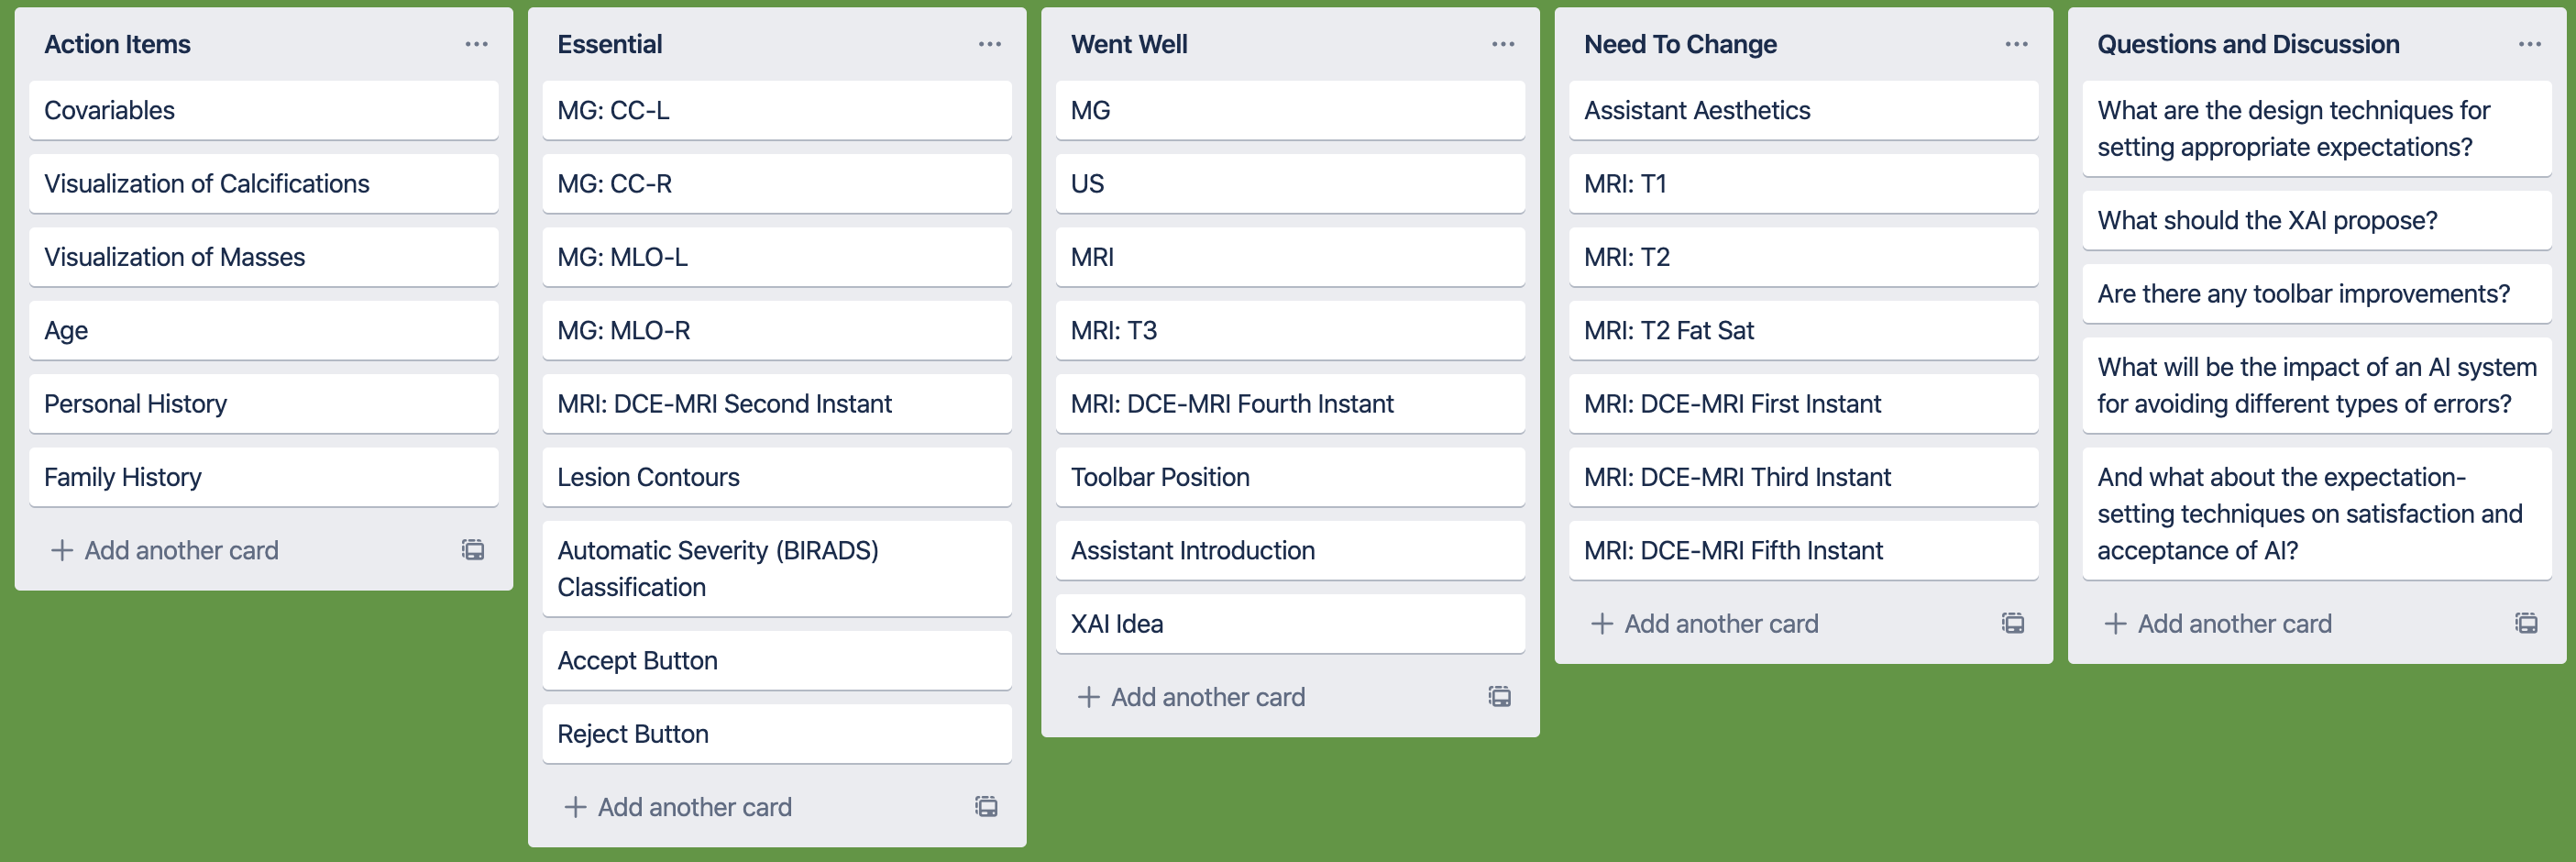
\includegraphics[width=\columnwidth]{images/fig039}
\caption{Resulting affinity diagrams passed to a digital software tool. The overall ideas and functionalities for categorization. Each idea and functionality has a category ({\it e.g.}, ``Action Items'', ``Essential'', ``Went Well'', ``Need To Change'' or ``Questions and Discussion''), so that it can manage the final requirements and development priorities of the {\it Assistant}.}
\label{fig:fig039}
\end{figure}
%%%%%%%%%%%%%%%%%%%%%%%%%%%%%%%%%%%%%%%%%%%%%%%%%%%

\textcolor{revised}{These ideas, functionalities, and priorities were then systematically translated into a digital format\footnotemark[7] using the collaborative tool.
Digital translation played a crucial role in streamlining data organization and enhancing collaboration among the research team.
It facilitated comprehensive insight capture and categorization, improving our data analysis's robustness.
Moreover, the flexibility of the digital format in modifying and reorganizing ideas was essential in adapting to evolving insights and feedback, a key aspect of the iterative \ac{UCD} process.}

%%%%%%%%%%%%%%%%%%%%%%%%%%%%%%%%%%%%%%%%%%%%%%%%%%%
\footnotetext[7]{For that, the collaboration software \href{https://trello.com}{Trello} (\href{https://trello.com}{trello.com}) was used, which allowed this study to organize and manage the group ideas digitally. The links were accessed on the 5th of April, 2023.}
%%%%%%%%%%%%%%%%%%%%%%%%%%%%%%%%%%%%%%%%%%%%%%%%%%%

\vspace{1.00mm}

\noindent
\textcolor{revised}{In this context, affinity diagrams~\cite{10.1145/3290605.3300628} played a crucial role by:}

\vspace{0.10mm}

\begin{enumerate}[(i)]
\item \textcolor{revised}{Categorizing items from the focus group, structuring the diverse inputs into coherent categories.}
\item \textcolor{revised}{Clustering chaotic and complex data, a common challenge in \ac{ML} projects~\cite{10.1145/2858036.2858373, 10.1145/3343413.3377983}, into manageable and interpretable groups.}
\end{enumerate}

\vspace{0.10mm}

\textcolor{revised}{Our methodology adeptly navigated the complexities of chaotic data analysis in medical imaging diagnosis.
By integrating affinity diagrams, we organized complex data and ensured continual alignment with clinician feedback.
This approach facilitated an iterative cycle where designs were consistently refined based on evolving insights, crucial for developing \ac{AI}-assisted diagnostic tools that are technically robust and clinically relevant, especially in breast cancer diagnosis.
The use of affinity diagrams thus became a pivotal element in our research, transcending data organization to reinforce a user-focused trajectory, ensuring that every stage of development resonated with the practical needs of clinicians.}

\textcolor{revised}{During the workshops (Section~\ref{sec:chap005003003001}), participants, encompassing both researchers and clinicians, were deeply engaged in the affinity diagramming process within the focus groups (Section~\ref{sec:chap005003003002}).
This collaborative effort involved critically reviewing and repositioning ideas and functionalities within various categories.
Initially grouped under the ``Action Items'' component, each concept or functionality was subject to a rigorous re-evaluation and re-categorization, facilitated by inclusive group discussions.
This methodical approach fostered a deeper understanding of the clinicians' perspectives and encouraged diverse viewpoints, enriching the design process with multifaceted insights.}

\textcolor{revised}{The iterative process was a conscious implementation of \ac{UCD} principles, aimed at ensuring the design's continuous alignment with clinicians' real-world needs and insights.
Embedding \ac{UCD} principles centrally within our methodology ensured that each element of the design was closely aligned with and shaped by the viewpoints of end-users.
This approach markedly improved the practicality and user-friendliness of our solutions in clinical settings.
Moreover, adopting these principles fostered a dynamic design environment, where feedback was actively sought and incorporated, resulting in a product that genuinely resonates with its intended users.}

% \vspace{2.5mm}

\noindent
For instance, several clinicians listed\footnotemark[8] their preferred components as the position (32/45) and simplicity (28/45) of the {\it Toolbar} (Section~\ref{sec:chap005004002}):

%%%%%%%%%%%%%%%%%%%%%%%%%%%%%%%%%%%%%%%%%%%%%%%%%%%
\footnotetext[8]{The workshop answers and feedback were transcribed so that they can join with similar opinions in different items. A ``(32/45)'' means that 32 clinicians for a total of 45 clinicians appointed a similar sentence of the clinician number 30, {\it i.e.}, ``(C30)'' on that example.}
%%%%%%%%%%%%%%%%%%%%%%%%%%%%%%%%%%%%%%%%%%%%%%%%%%%

\vspace{2.50mm}

\noindent
``{\it The {\bf Toolbar} position should be on the top in contrary to what we usually see}.'' (C30)

\vspace{2.50mm}

\textcolor{revised}{In this phase, we created a labeled ``Toolbar Position'' item, which underwent evaluation by the clinicians.
Most clinicians endorsed this item, leading to its placement in the ``Went Well'' category, indicative of positive reception.
This categorization reflected our \ac{UCD} principle of iterative design, where clinician feedback directly influenced the design process.
The minority who rejected or omitted the item offered insights for refinement, showcasing the dynamic, responsive nature of our \ac{UCD} approach.}

\vspace{1.00mm}

\noindent
Through the affinity diagrams, it was found that specific items, within each own categories, correspond to three needs of clinicians:

\vspace{0.10mm}

%%%%%%%%%%%%%%%%%%%%%%%%%%%%%%%%%%%%%%%%%%%%%%%%%%%
\begin{enumerate}[label=\alph*]
\item - new strategies among the medical imaging visualizations;
\item - to understand the intelligent agent ({\it Assistant}) result; and
\item - to control ({\it e.g.}, {\it accept} or {\it reject}) the final intelligent agent ({\it Assistant}) result.
\end{enumerate}
%%%%%%%%%%%%%%%%%%%%%%%%%%%%%%%%%%%%%%%%%%%%%%%%%%%

\vspace{0.10mm}

These threefold clinicians' needs were possible to achieve due to the correct application of affinity diagrams.
The technique was of chief importance to promote an understanding of this thesis background (Chapter~\ref{chap:chap002}).
Without such an approach, it would be impossible to follow the proper design of the developed intelligent agent.
Furthermore, the technique will follow all the steps and iterations that will be important for the future directions of this thesis (Section~\ref{sec:chap007004} of Chapter~\ref{chap:chap007}).

\textcolor{revised}{During the focus group sessions, clinicians emphasized the necessity to comprehensively map out all {\it workflow} processes and activities integral to the diagnostic pipeline.
This discussion underscored the significance of integrating \ac{AI} systems tuned to these specific {\it workflow} characteristics, thereby augmenting their clinical tasks.
This aspect of the research aligns with the \ac{UCD} approach, where understanding and incorporating user workflows is crucial in designing effective \ac{AI} tools.}

\vspace{1.50mm}

\noindent
One clinician even stated that an intelligent agent would make their job more straightforward:

\vspace{2.50mm}

\noindent
``{\it If we have an assistant like this in our workflow, it will be more simple and easy to do our job.}'' (C45)

\vspace{1.50mm}

\textcolor{revised}{This statement aligns with \acs{UCD}'s primary goal: simplifying and improving the user experience.
The identified needs to cover essential preconditions for prompt, accurate diagnosis, highlighting a user-centric approach in \ac{AI} system development.
Focusing on these needs ensured our research followed \ac{UCD} principles, making the intelligent agent's design and implementation responsive to clinicians' real-world requirements.}

Throughout this process, a set of design guidelines have been derived.
To investigate how the clinical {\it workflow} proceeds, affinity diagrams were used to connect ideas and functionalities to a set of guidelines that will be described next.
For this purpose, three central design components were created that can be applied for medical imaging systems with \ac{AI} behind:
(i) highlighting the essential lesion regions;
(ii) explaining the \ac{AI} results for higher interpretability; and
(iii) providing control of the final result.
As follows, these three design components are translated into four design guidelines.

\vspace{2.00mm}

\noindent
From Figure~\ref{fig:fig039} and from the feedback obtained when building the affinity diagrams, the following design guidelines were considered:

\vspace{1.50mm}

%%%%%%%%%%%%%%%%%%%%%%%%%%%%%%%%%%%%%%%%%%%%%%%%%%
\begin{description}
\item[Relevance to Diagnostic] - the \ac{AI} system ({\it Assistant}) should provide additional relevant clinical information so that clinicians can explore more granular details of the diagnosis.
For instance, information that allows clinicians to understand the relevant lesions (Figure~\ref{fig:fig032}) and the respective severity levels regarding both the shape and size of the lesion.

\vspace{1.50mm}

\item[Clinician-Centered Activities] - since data must be shared between clinicians, the \ac{AI} system should be designed to mimic collaboration.
For instance, clinicians should be able to remotely visualize the same lesion annotation synchronously.
This means the \ac{AI} system should support and enhance activities that facilitate discussion, leading to more robust decision-making.

\vspace{1.50mm}

\item[Provide Explanations] - the system must provide answers regarding the final \ac{AI} result.
In this work, an ``Explain'' button (Figure~\ref{fig:fig040}) was created so that clinicians can open the heatmaps (Figure \ref{fig:fig032}) on the image to explain the \ac{AI} recommendations.
The heatmaps will show the variability (color) of the important regions, which is information that will explain the final \ac{BI-RADS}.

\vspace{1.50mm}

\item[Feeling in Control] - the {\it Assistant} must provide control for the final decision. Clinicians must feel that, in case of a wrong \ac{AI} diagnostic, the final result must be changed ({\it reject}) by them so that we can guarantee the patient's safety and the right classification of the lesion.
\end{description}
%%%%%%%%%%%%%%%%%%%%%%%%%%%%%%%%%%%%%%%%%%%%%%%%%%

\vspace{2.00mm}

\textcolor{revised}{To summarize, clinicians envision a transformation in their work processes as \ac{AI} tools integrate into breast cancer diagnosis.
This evolution requires comprehensive training for their adjustment to new \acs{AI}-augmented workflows and decision-making.
The collaboration between clinicians and \ac{AI} continuously refines itself through ongoing learning from new data, progressively improving diagnostic accuracy and efficiency.
In this section (Section~\ref{sec:chap005003003004}), we delve into the key role of data clustering within our research methodology.
Clustering, guided by the inherent `affinity' among collected ideas and functionalities, proves indispensable in uncovering common themes and patterns in the data, aligning seamlessly with established \ac{UCD} methodologies for informed design decisions~\cite{10.1145/3290605.3300234, 10.1145/3313831.3376718}.
In our \ac{UCD} approach, this clustering efficiently distills data from interviews and workshops into essential design components for medical imaging systems with \ac{DL} methods, ensuring user needs shape the design of intelligent agents.}

\subsubsection{Essential Data}
\label{sec:chap005003003004}

Analyzing the essential data is vital for the developed \ac{UI}.
Indeed, the \ac{MRI} data is inherently chaotic since each exam contains tens of volumes.
The volumes can be part of several sequences\footnotemark[9] for the \ac{MRI} modality.
Thus, designing a comprehensive visualization for such chaotic data is necessary.

\vspace{1.00mm}

\noindent
Specifically, for the medical imaging background (Chapter~\ref{chap:chap002}), the following \ac{MRI} characteristics were addressed:

\vspace{0.05mm}

%%%%%%%%%%%%%%%%%%%%%%%%%%%%%%%%%%%%%%%%%%%%%%%%%%
\begin{multicols}{4}
\begin{enumerate}
\item T1;
\item T2;
\item T2 Fat-Sat;
\item T2 TIRM;
\item Diffusion;
\item DCE MIP;
\item DCE WO;
\item DCE PEI;
\end{enumerate}
\end{multicols}
%%%%%%%%%%%%%%%%%%%%%%%%%%%%%%%%%%%%%%%%%%%%%%%%%%

\vspace{0.05mm}

\textcolor{revised}{To address the ``chaotic data problem'' in our work, affinity diagramming was utilized~\cite{harrington2016affinity}.
The method streamlined the organization of notes by clustering them according to shared topics, thereby forming structured data groups.
Through an iterative process of labeling and clustering, we distilled the information into a few high-level groups.
These groups were crucial for pinpointing prevalent issues and viable solutions.
Employing this structured approach proved pivotal in delineating user needs and design challenges, ultimately guiding the design and development of the intelligent agent.}

\textcolor{revised}{During focus groups (Section~\ref{sec:chap005003003002}), participants pinpointed several user needs and requirements deemed essential (as shown in the ``Essential'' column of Figure~\ref{fig:fig039}).
These insights were critical in defining the most pertinent modalities and procedures for the medical imaging workflow (Figure~\ref{fig:fig018}).
Given the plethora of \ac{MRI} sequences available, clinicians often grapple with the challenge of visualizing all volumes effectively.
Identifying the \ac{MRI} volumes that align closely with clinicians' needs was thus imperative.
This identification was facilitated by the affinity diagrams, which distilled user needs and requirements, helping to define essential modalities and procedures for the workflow.}

%%%%%%%%%%%%%%%%%%%%%%%%%%%%%%%%%%%%%%%%%%%%%%%%%%
\footnotetext[9]{As the most sensitive method for detection of breast cancer (\href{https://radiopaedia.org/articles/breast-mri?lang=us}{radiopaedia.org/articles/breast-mri}), the breast MRI aims to obtain a reliable evaluation of any lesion within the breast. However, the modality relies on several sequence options, such as: (1) T1 (longitudinal relaxation time), the time constant which determines the rate at which excited protons return to equilibrium; (2) T2 (transverse relaxation time), similar to T1, but with the second time constant; (3) T2 Fat-Sat, pulses are short-duration tuned to the resonance frequency of fat; (4) T2 Turbo Inversion Recovery Magnitude (TIRM); (5) Diffusion, method that produces invivo MRI of tissues sensitized with the local characteristics of molecular diffusion; (6) DCE Maximum Intensity Projection (MIP); (7) DCE WithOut (WO) contrast agent; and (8) DCE Positive Enhancement Integral (PEI). Although they are more, these were the MRI sequence options used by the nine institutions. Nevertheless, it is important to underline that the MRI volumes are always used as an adjunct to the standard diagnostic procedures of the breast, {\it i.e.}, clinical examination, MG and US.}
%%%%%%%%%%%%%%%%%%%%%%%%%%%%%%%%%%%%%%%%%%%%%%%%%%

We also observed that clinicians from different hospitals had different preferences for \ac{MRI} sequences.
However, since the medical imaging data used was from the \acs{HFF} clinical institution, their main sequence (\acs{DCE-MRI} in a second instant) was chosen as the standard.
Through data clustering, the need for each modality (\acs{MG}, \acs{US} and \acs{DCE-MRI} at the second time instant) and its meaning to the clinical workflow (Figure~\ref{fig:fig018}) were identified.
The workshops (Section~\ref{sec:chap005003003001}) and focus groups (Section~\ref{sec:chap005003003002}) helped to gather essential data on how these modalities can provide complementary information for a reliable diagnosis, tailored to each institution's needs.

\subsubsection{Prototype Requirements}
\label{sec:chap005003003005}

% \vspace{2.50mm}

\noindent
\textcolor{revised}{In adherence to our human-centered design philosophy, the development of the \ac{AI}-assisted prototype was guided by two principal objectives:}

\vspace{1.00mm}

%%%%%%%%%%%%%%%%%%%%%%%%%%%%%%%%%%%%%%%%%%%%%%%%%%

\begin{enumerate}
\item \textcolor{revised}{\textbf{Enhanced Diagnostic Capabilities through Multi-Modal Medical Imaging:} The prototype integrates a suite of functionalities specifically designed to assist clinicians.
These tools, prioritized during our iterative design interventions, aim to augment the diagnostic process by leveraging the strengths of multi-modal imaging.}
\item \textcolor{revised}{\textbf{Automated Severity Assessment of Lesions:} Incorporating a DenseNet architecture, the prototype functions as an anthropomorphic intelligent agent.
This agent is responsible for providing \ac{BI-RADS} scores and detailed explanations, thereby enhancing the interpretability and reliability of lesion severity classification.}
\end{enumerate}

%%%%%%%%%%%%%%%%%%%%%%%%%%%%%%%%%%%%%%%%%%%%%%%%%%

\vspace{1.00mm}

\textcolor{revised}{The iterative design process, encompassing workshops and focus groups, facilitated a deeper engagement with clinicians, enabling us to garner valuable insights and feedback.
This participatory approach was instrumental in refining the prototype to better align with clinical needs.
For example, a significant modification, based on clinician feedback, involved repositioning the \ac{UI} of the intelligent agent.
Originally positioned at the upper and central part of the display, the \ac{UI} was repositioned to the lower right corner within the {\it Viewports} ({\it Re-5.1.} of Figure~\ref{fig:fig040}).
This adjustment was determined to be more user-friendly and less disruptive to the clinical workflow.}

\textcolor{revised}{With a direct outcome from our design process, this relocation is anticipated to enhance clinicians' efficiency in decision-making and reduce the time required for patient diagnosis.
Furthermore, it addresses the potential for reducing medical errors.
The decision to integrate the {\it Assistant} ({\it Re-6.} of Figure~\ref{fig:fig040}) avatar within the {\it Viewports} ({\it Re-5.1.} of Figure~\ref{fig:fig040}) was driven by the need for seamless accessibility and minimal disruption to the clinicians' established workflow patterns.
This integration exemplifies \ac{UCD} principles, with iterative feedback and testing crucial in evolving the design to meet user needs.
In the subsequent Section~\ref{sec:chap005003004}, we explore how these design choices enhance breast cancer diagnosis through intelligent agent integration.}

\textcolor{revised}{Anticipating that these recommendations will enhance clinicians' decision-making efficiency, as well as reduce diagnostic time and medical errors, our design activities led to significant conclusions (Section~\ref{sec:app003004005} of Appendix~\ref{chap:app003}).
In summary, the strategic placement of the {\it Assistant} avatar ({\it Re-6.} of Figure~\ref{fig:fig040}) within the {\it Viewports} ({\it Re-5.1.} of Figure~\ref{fig:fig040}) ensures easy accessibility, aligning with clinicians' usual workspace and reducing interaction time.
This placement highlights our commitment to user-centric design, ensuring the tool meets clinical needs and integrates smoothly into the existing workflow.
By focusing on \ac{UX} enhancement, we aim to improve the acceptance and effectiveness of \ac{AI}-assisted diagnostic tools, contributing to more efficient and accurate medical assessments.}

% \vspace{2.50mm}

\noindent
\textcolor{revised}{Because of that, this design choice addresses visibility concerns in two ways:}

\vspace{1.00mm}

%%%%%%%%%%%%%%%%%%%%%%%%%%%%%%%%%%%%%%%%%%%%%%%%%%

\begin{enumerate}[(a)]
\item \textcolor{revised}{Primarily, the majority of \ac{MG} and \ac{MRI} imaging modalities typically do not display critical information in the lower right area of the {\it Viewports} ({\it Re-5.1.} of Figure~\ref{fig:fig040}), where the avatar is positioned.}
\item \textcolor{revised}{Additionally, we integrated a feature enabling the {\it Assistant} avatar ({\it Re-6.} of Figure~\ref{fig:fig040}) to be temporarily hidden via a discreet button.
This ensures clinicians have an unobstructed view of the entire image when needed, preserving the diagnostic process's integrity.}
\end{enumerate}

%%%%%%%%%%%%%%%%%%%%%%%%%%%%%%%%%%%%%%%%%%%%%%%%%%

\vspace{1.00mm}

\textcolor{revised}{These user-centered design adaptations (detailed in Section~\ref{sec:app003003001}) not only make the intelligent agent more accessible, but also seamlessly integrate it into the clinicians' existing workflow.
This integration is a testament to the application of \ac{UCD} principles, emphasizing iterative feedback and refinement in developing \acs{AI}-assisted tools.
In the following Section~\ref{sec:chap005003004}, we are further exploring the integration of \acs{AI}-assisted methods in the design of intelligent agents.
Specifically, we will examine how the {\it BreastScreening-AI} design contributes to mitigating challenges in breast cancer diagnosis, aligning with overarching healthcare design objectives.}

\subsection{Design Goals}
\label{sec:chap005003004}

In this section, it is investigated how \ac{AI}-assisted methods could be integrated into the design of an intelligent agent for the medical imaging diagnostic on breast cancer.
The purpose is to help mitigate breast cancer diagnosis, while meeting overall design goals.
This solution provides an absolute scale for clinicians' performance and leads to the instrumentation of the hereby design goals and constrains.
With the introduction of intelligent agents, the designed {\it BreastScreening-AI} framework~\cite{CALISTO2021102607} dictated a departure from the later {\it BreastScreening} annotating tool~\cite{10.1145/3399715.3399744} wrapping approach of \ac{AI} techniques, toward a new communication that only exposes the required patient information, as well as lesion classification and segmentation functionalities (Appendix~\ref{chap:app008}).

The {\it BreastScreening-AI} framework is designed to reduce the burden of usage and expand clinicians' performance by simplifying the complexities that are frequently encountered when clinicians are diagnosing a patient.
Here, the main goal is to expose the \ac{AI} algorithm results in a readily available format~\cite{CALISTO2022102285}.
The design goals of {\it BreastScreening-AI} have been for a robust, reliable, and elegant \ac{UI} to promote the integration of intelligent agents in the \ac{RRR} workflow.

The main design goals are closely related to the research insights and challenges of the previous section (Section~\ref{sec:chap005003002}), namely:
(1) collection of a \ac{GT} annotations, {\it i.e.}, masses in all imaging modalities and microcalcification lesions in \ac{MG} (for both \ac{CC} and \ac{MLO} views);
(2) classification of the lesion severity using the \ac{BI-RADS}~\cite{aghaei2018association};
(3) categorization of the breast tissues (dense vs non-dense);
(4) clinical co-variables, such as personal and family records; and
(5) visualizations for clinical summary which are crucial for a proper diagnosis and to perform patient follow-up.

% \vspace{1.50mm}

\noindent
These five insights were fused into three corresponding design goals, as follows:

\vspace{1.00mm}

%%%%%%%%%%%%%%%%%%%%%%%%%%%%%%%%%%%%%%%%%%%%%%%%%%
\begin{description}
\item[\ac{MID}] focusing on how to provide the best visualization strategy, given the heterogeneous information coming from the multi-modal nature of the information;

\vspace{0.50mm}

\item[\ac{CRD}] focusing on improving the clinician's ability to {\it accept} or {\it reject} the \ac{AI}-assisted results;

\vspace{0.50mm}

\item[\ac{EXD}] focusing on increasing physician's understanding of how the \ac{AI} techniques operate. By increasing understanding of how \ac{AI} works, physicians can update their expectations of how well and in which situations the system is likely to work;
\end{description}
%%%%%%%%%%%%%%%%%%%%%%%%%%%%%%%%%%%%%%%%%%%%%%%%%%

\vspace{1.50mm}

Until now, this is the first attempt to holistically integrate these design goals in the context of medical imaging diagnosis supported by \ac{AI}-assisted methods.
Through user studies, it was identified the above three ({\it i.e.}, \ac{MID}, \ac{CRD} and \ac{EXD}) design goals.
Next, the document will describe the {\it BreastScreening-AI} framework~\cite{CALISTO2021102607} taking into account these design goals.

\section{BreastScreening-AI}
\label{sec:chap005004}

To validate the proposed design goals, a prototype called {\it BreastScreening-AI} framework was developed~\cite{CALISTO2021102607}.
As a proof-of-concept fully functional prototype, this tool aims to be evaluated in a realistic clinical scenario.
In the following sections, the document will describe the main functionalities for prototyping the {\it BreastScreening-AI} framework.
Next, the document describes the prototype details and system implementation.

\subsection{Implementation}
\label{sec:chap005004001}

Similar to an earlier version, the {\it BreastScreening-AI} framework was implemented using \href{https://cornerstonejs.org/}{CornerstoneJS} with a \href{https://nodejs.org/}{NodeJS} server.
Once the set of medical images is loaded in the visualization viewport (Figure \ref{fig:fig040}) the user can interact with the data by manipulating the visualization through the mouse and keyboard.
For instance, rolling the mouse wheel to navigate across the volume slices (\acs{MRI}) or even moving the mouse to drag-and-drop the several modalities to the viewport.
The goal of the proposed multi-modal strategy is then to provide the visualization and manipulation of several modalities, comparing lesion patterns among medical images.

Due to the integration of intelligent agents, the new developments of the {\it BreastScreening-AI} prototype were giving this thesis the opportunity to test properly what are the implications of \ac{AI} techniques on the \ac{RRR} workflow.
Such implications are achieved through the implementation and integration of a classifier model (DenseNet) into the designed \ac{UI}~\cite{maicas2018training}.
By showing the work design decisions, the following sections will cover these prototyping directions.

%%%%%%%%%%%%%%%%%%%%%%%%%%%%%%%%%%%%%%%%%%%%%%%%%%%
\begin{figure}[htbp]
\centering
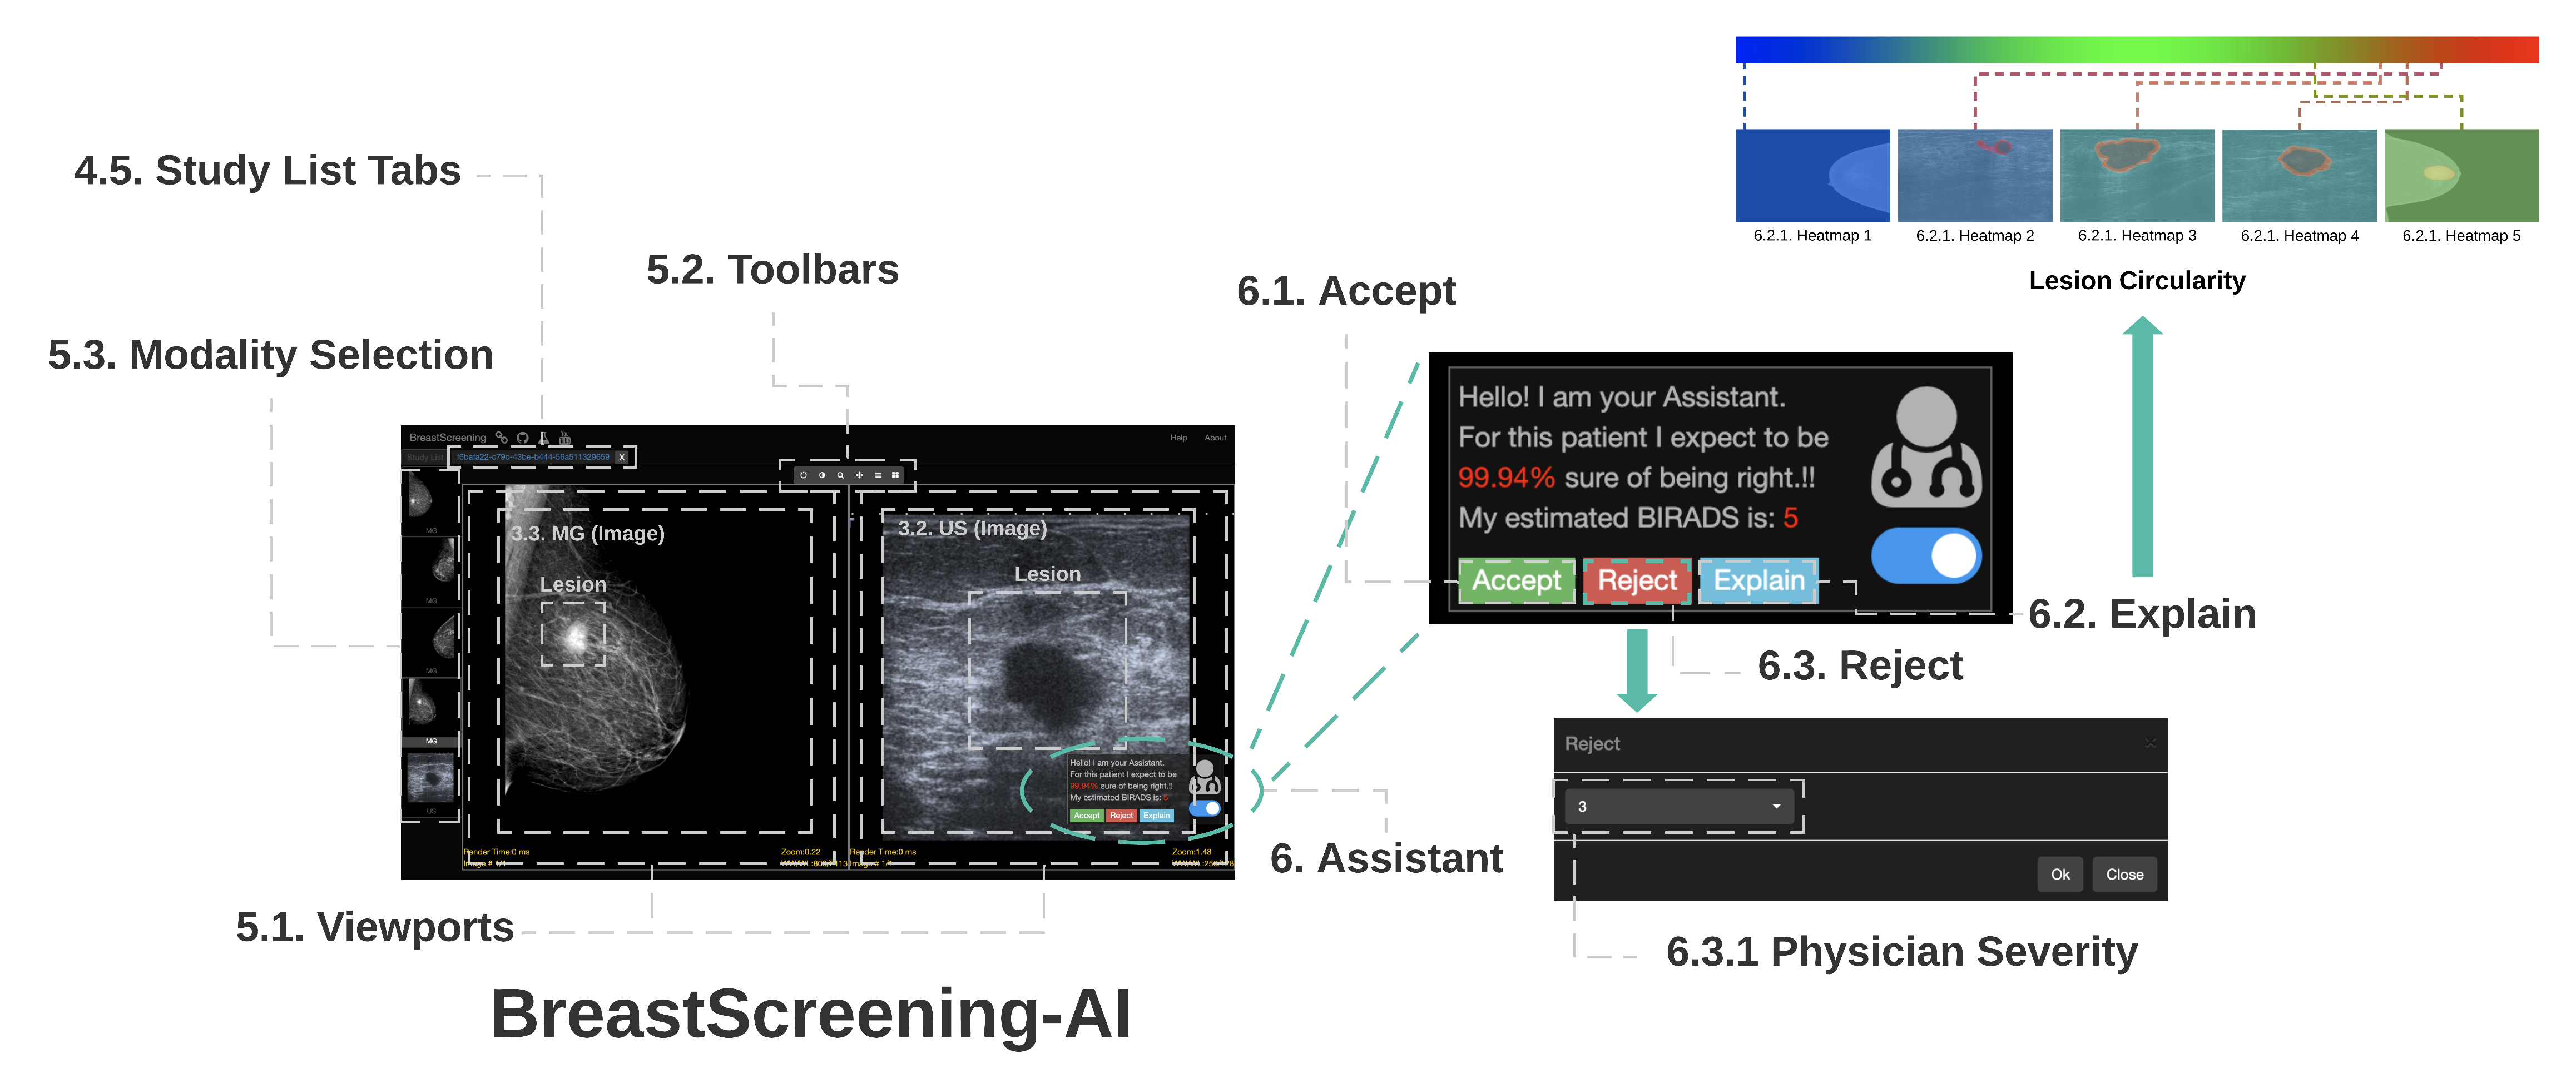
\includegraphics[width=\textwidth]{images/fig040}
\caption{\textcolor{revised}{The proposed {\it BreastScreening-AI} provides several functionalities. Specifically, it is possible to validate the DenseNet output classification along with radiologists. The system is framed in the following subcategories: Study List Tabs (Re-4.5.); Viewports (Re-5.1.); Toolbars (Re-5.2.); Modality Selection (Re-5.3.); Assistant (Re-6.); Accept (Re-6.1.); Explain (Re-6.2.); Reject (Re-6.3.); and Physician Severity (Re-6.3.1.). On Explain (Re-6.2.), the assistant will pop-up several heatmaps. The proposed model has two main stages: (i)  first it computes the BI-RADS, based on the output classification of the DenseNet; and (ii) it computes the size and circularity of the lesion based on the heatmaps.}}
\label{fig:fig040}
\end{figure}
%%%%%%%%%%%%%%%%%%%%%%%%%%%%%%%%%%%%%%%%%%%%%%%%%%%

\subsection{User Interface}
\label{sec:chap005004002}

In this section, we describe the design and implementation of the \ac{UI} for the {\it BreastScreening-AI} prototype based on identified user needs (Section~\ref{sec:chap005003003}).
The \ac{UI} includes a set of refinement mechanisms to guide clinicians during the diagnostic process (Figure~\ref{fig:fig040}), comprising two main components:
(1) the list of patients; and
(2) medical imaging views.
The \textcolor{revised}{{\it List of Patients Views} ({\it Re-4.})} include a \textcolor{revised}{{\it List of Patients} ({\it Re-4.1.})} with the most important and required information for clinicians.
From here, users can search all patients using criteria such as {\bf Patient ID}, {\bf Study Date}, available {\bf Modality} sets, {\bf Study Description}, and number of {\bf Images}.
The \textcolor{revised}{{\it Study List Tabs} ({\it Re-4.5.})} allow clinicians to switch between diagnosed patients and medical imaging diagnosis views.
The \ac{UI} is also informing clinicians about how to classify and use the system, where we designed the \textcolor{revised}{{\it Toolbars} ({\it Re-5.2.})} functionality to match the user's requirements, and \textcolor{revised}{{\it Viewports} ({\it Re-5.1.})} to process the image by using \textcolor{revised}{{\it Toolbars} ({\it Re-5.2.})} provided functionalities.
In the end, \textcolor{revised}{inserting the \ac{BI-RADS} use case was held by the {\it Physician Severity} ({\it Re-6.3.1.}) functionality}, allowing clinicians to classify the severity of the breast lesion for each patient.

Overall, this section describes the design and implementation of the \ac{UI} for prototyping the first iterations of the {\it BreastScreening-AI} framework.
Specifically, it includes refinement mechanisms to guide clinicians during the diagnostic process.
The following sections will map the two main \ac{UI} functionalities, {\it i.e.}, assistant (Section~\ref{sec:chap005004002001}) and explainability (Section~\ref{sec:chap005004002002}), between the design goals (Section~\ref{sec:chap005003002}) under this thesis.

\subsubsection{Assistant}
\label{sec:chap005004002001}

\textcolor{revised}{Figure~\ref{fig:fig040} shows the {\it Assistant} ({\it Re-6.}) with its {\it Accept} ({\it Re-6.1.}) and {\it Reject} ({\it Re-6.3.}) functionalities, enabling clinicians to directly control the \ac{DNN} classifications derived from the DenseNet model~\cite{Huang_2017_CVPR}.
However, integrating a \ac{DNN} needs special attention (Appendix~\ref{chap:app004}).
Typically, the training of a \ac{DNN} is expensive regarding the time spent (Section~\ref{sec:app004001}), since its classification performance will improve as the training dataset becomes larger.
Thus, training the model from scratch is not the best option.
For this reason, we pre-train ({\it i.e.}, off-line training before the \ac{UI} integration) the \ac{DNN} on the ImageNet dataset~\cite{10.1145/3351095.3375709} and fine-tuned using our multi-modal breast dataset (Section~\ref{sec:app004005}).
Specifically, we fine-tune the \ac{DNN} using supervised learning.
Only afterwards, the pre-trained DenseNet is incorporated into the \ac{UI}.}

The implemented DenseNet takes medical images as an input and outputs the severity probability.
The input consists of images ({\it i.e.} \ac{MG}, \ac{US} and \ac{MRI} slices) with the corresponding label ({\it i.e.}, the \ac{BI-RADS}) that is previously classified by an expert.
The output consists of having five nodes in the last layer of the \ac{DNN}.
Each node is assigned to a given class that corresponds to each \ac{BI-RADS} score.
After this stage, we have conditions for the integration, since now the DenseNet is tuned to perform the classification in unseen test images.
The classification is fast, being tailored for an online diagnosis.

\textcolor{revised}{When several modalities (\ac{MID} and \ac{CRD}) are correctly used, regarding the {\it Modality~Selection} ({\it Re-5.3.}) on a multimodality view, the clinician can find more accurately the right severity classification, as concluded in Section~\ref{sec:app003003002} of Appendix~\ref{chap:app003}.
For the {\it Reject} ({\it Re-6.3.}) option, the physician will have the opportunity to insert (\ac{CRD}) the proposed \ac{BI-RADS} on a drag-and-drop menu of severity options by using the {\it Physician Severity} ({\it Re-6.3.1.}) functionality.
Both \ac{MID} and \ac{CRD} goals are supporting our {\bf RQ5.1} question (Section~\ref{sec:chap005001002}).}

\subsubsection{Explainability}
\label{sec:chap005004002002}

\textcolor{revised}{Finally, the clinician may press for the {\it Explain} ({\it Re-6.2.}) functionality  by looking at the generated heatmaps (Figure~\ref{fig:fig032}).
The generation of the above colour maps come from the following information:
(i) the area ({\it Lesion Size}) of the lesion that comes from the delineation process,
(ii) the circularity/sharpness ({\it Lesion Shape}) that can be computed from the annotation in (i), and
(iii) the \ac{BI-RADS} score automatically provided by the DenseNet ({\it i.e.}, classifier intelligent agent).
The \ac{EXD} design goal is performed as above described helping to answer to research questions {\bf RQ5.2} and {\bf RQ5.3} (Section~\ref{sec:chap005001002}).}

Covered by the \ac{EXD} design goal, the thesis can provide a key component to disambiguate the \ac{AI} result with the application of an explanation technique (Section~\ref{sec:chap003007}).
For a better prediction, the result of this explanation process is a heatmap visualizing the importance of each pixel.
With heatmaps, clinicians can capture and understand the logic arguments of the DenseNet (Section~\ref{sec:chap005006002}) by giving images and pixels a color meaning of the lesion severity.
Thus, the \ac{EXD} design goal is bringing the opportunity to disambiguate this \ac{DL} method for a more transparent and explainable (\ac{XAI}) process.


%%%%%%%%%%%%%%%%%%%%%%%%%%%%%%%%%%%%%%%%%%%%%%%%%%%
\begin{figure}[htbp]
\centering
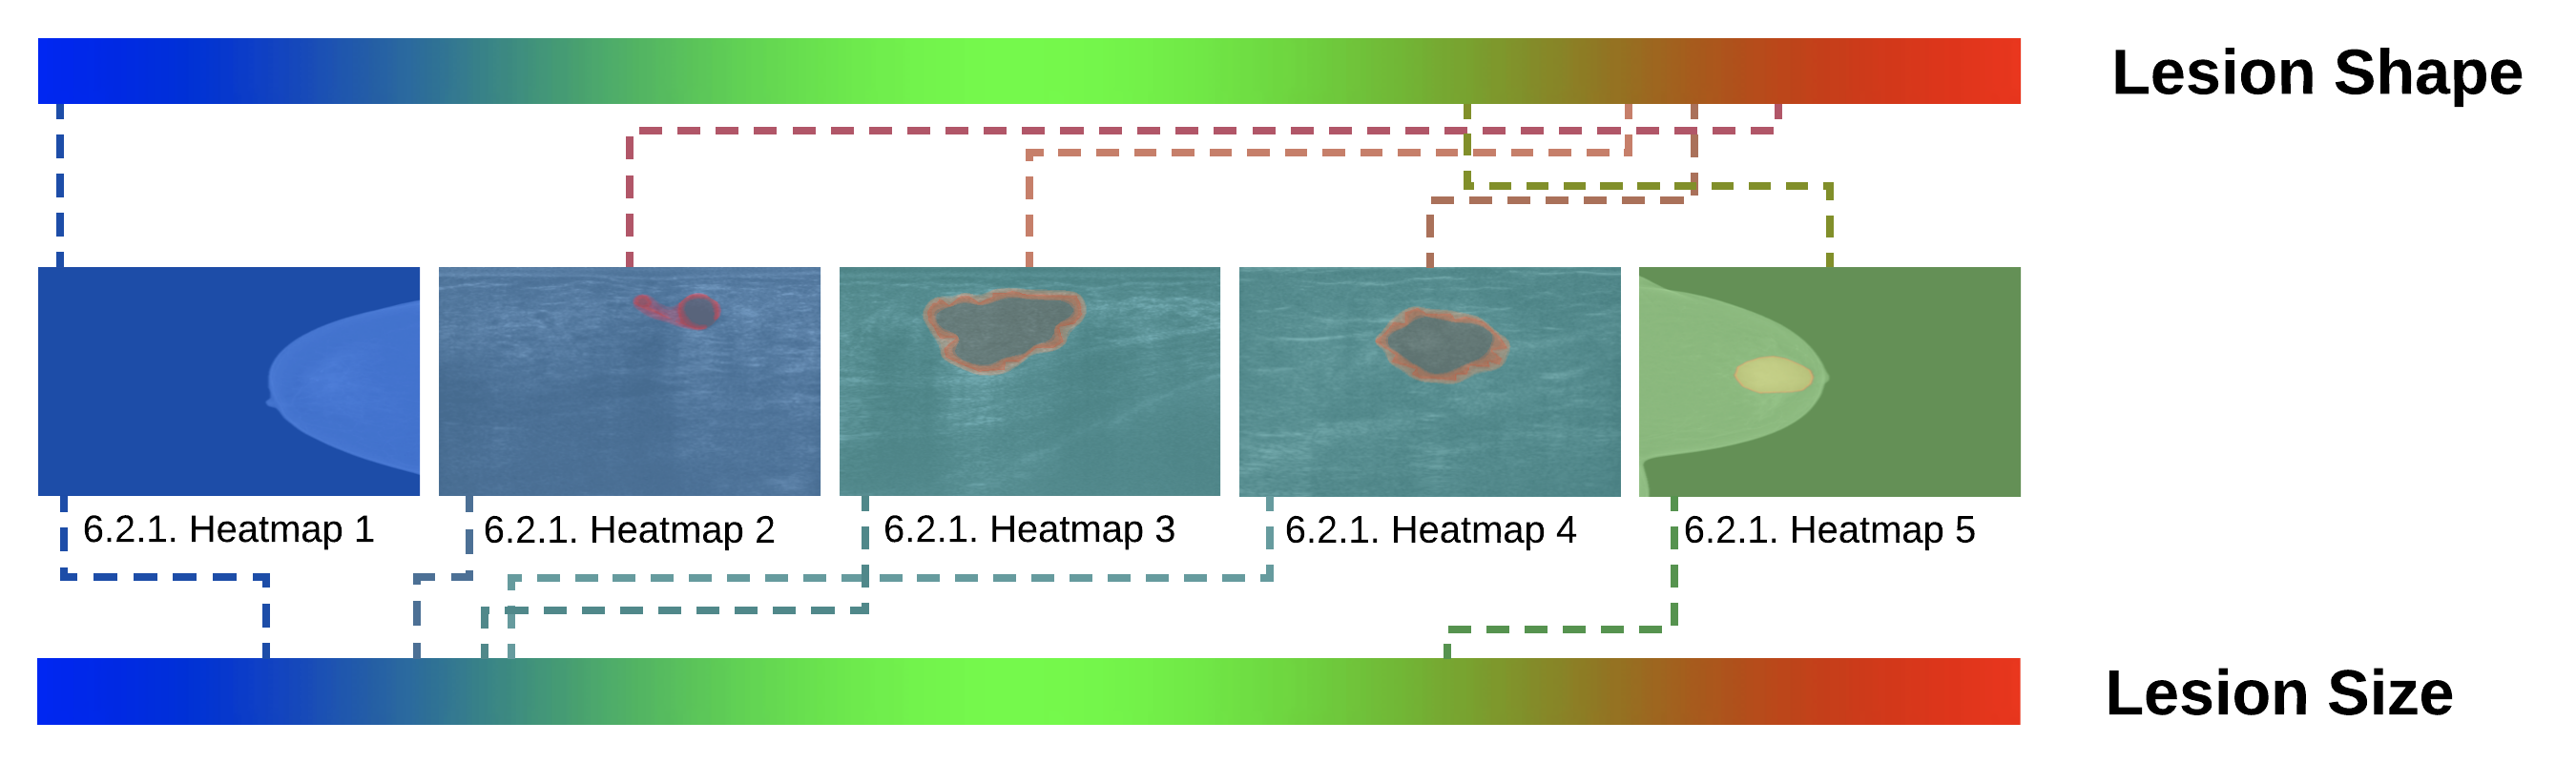
\includegraphics[width=\columnwidth]{images/fig032}
\caption{On Explain (Re-6.2.), the assistant will pop-up several {\it heatmaps}. The {\it heatmaps} represent two different scales: (a) {\it Shape}; and (b) {\it Size} of the lesion. First, the model computes the BI-RADS using the DenseNet classification. Second, the model computes the lesion circularity (top scale) and size (bottom scale) and associate it to the colors regarding both circularity/size and BI-RADS.}
\label{fig:fig032}
\end{figure}
%%%%%%%%%%%%%%%%%%%%%%%%%%%%%%%%%%%%%%%%%%%%%%%%%%%

\section{Methods}
\label{sec:chap005005}

For this study, an evaluation of {\it BreastScreening-AI} simulating real-world conditions with 45 clinicians, within-subject, in nine different clinical institutions was conducted.
The study goal was to quantitatively and qualitatively assess the proposed design principles that the {\it BreastScreening-AI} embodies, and to understand how these principles would work in practice.
The experimental setup aimed at testing two conditions: {\bf Clinician-Only} ({\it Current}) -- simulating clinicians' {\it current} setup, equal to what they have in their clinical institutions, {\it i.e.}, a multimodality strategy without any \ac{AI}-assisted technique; {\bf Clinician-AI} ({\it Assistant}) -- multimodality strategy taking advantage of the \ac{AI}-assisted ({\it e.g.}, DenseNet~\cite{9098470}), supporting clinician's second opinion and autonomous patient diagnostic.

\vspace{2.00mm}

\noindent
For each condition, three classes of patients were defined:

%%%%%%%%%%%%%%%%%%%%%%%%%%%%%%%%%%%%%%%%%%%%%%%%%%%
\begin{itemize}
\item {\bf Class 1}: patients such that \ac{BI-RADS} $\leq$ 1 (low severity);
\item {\bf Class 2}: patients such that 1 $<$ \ac{BI-RADS} $\leq$ 3 (medium severity);
\item {\bf Class 3}: patients such that \ac{BI-RADS} $>$ 3 (high severity);
\end{itemize}
%%%%%%%%%%%%%%%%%%%%%%%%%%%%%%%%%%%%%%%%%%%%%%%%%%%

Having data available is challenging and requires multiple steps (Section~\ref{sec:app004002} of Appendix~\ref{chap:app004}), including anonymization of data.
The ideal approach is a collaboration between clinicians and \ac{AI} researchers, either in-house or through collaborative research agreements.
Therefore, a protocol was celebrated with \acs{HFF} so that the interchange of patients could be possible.
The purpose of this protocol is to establish bases of collaboration in all scientific and technological areas, as well as education and training in which \ac{IST} and \acs{HFF} carry out their activities.
From this protocol, the exams were annotated by eight radiologists and classified with a \ac{BI-RADS} severity from an expert doctor.
The expert doctor is the head of the radiologist services of the \acs{HFF} clinical institution.

\subsection{Participants}
\label{sec:chap005005001}

In this study, participants were asked to practice with three predefined sets of patients randomly selected from the three above classes.
To accomplish this, each patient was randomly selected ({\it i.e.}, {\bf P1}, {\bf P2} and {\bf P3}) from each class ({\it i.e.}, {\bf Class 1}, {\bf Class 2} and {\bf Class 3}), respectively.
Then, participants were asked to diagnose each patient.
A natural expectation is that the intelligent agent would minimize the time required and accuracy ({\it e.g.}, improving \ac{FP} or \ac{FN} values).
The study involved 45 clinicians, recruited on a volunteer basis from a broad range of clinical scenarios, including nine different health institutions (two public hospitals, two cancer institutes, one private hospital, and two private clinics).

\vspace{4.00mm}

\noindent
In the following list, the number of clinicians and respective clinical institutions is provided:

\vspace{2.00mm}

\begin{multicols}{2}
\begin{itemize}
\item 12 clinicians of \acs{HFF};  % HFF
\item 10 clinicians of \acs{IPOL}; %IPOL
\item 2 clinicians of \acs{HSM};   %HSM
\item 9 clinicians of \acs{IPOC};  %IPOC
\item 1 clinician of \acs{MMC};    %MMC
\item 1 clinician of \acs{SAMS};   %SAMS
\item 8 clinicians of \acs{HB};    %HB
\item 1 clinician of \acs{HSA};    %HSA
\item 1 clinician of \acs{JCCC}.   %JCCC
\end{itemize}
\end{multicols}

\vspace{2.00mm}

Before the experiment, clinicians first filled out a pre-study questionnaire eliciting demographic information (Appendix~\ref{chap:app006}), including age group, gender, and medical professional experience, among others.
From the demographic questionnaires:
24.4\% of the clinicians have between 31 and 40 years of practical experience (seniors);
31.1\% have between 11 and 30 years of experience (middles);
17.8\% have between 6 and 10 years of experience (juniors); and
26.7\% have limited experience (interns).
Interviews were conducted in a semi-structured fashion, taking about 30 minutes.
Overall, 57 days were spent on the clinical institutions for the observation process and six months for the classification.

\subsection{Apparatus}
\label{sec:app002005002}

To track user interactions across the evaluated system, we used the \hyperlink{https://www.hotjar.com/}{Hotjar} tool.
This tool is an analytic package allowing this study to follow users remotely.
It also provides two critical pieces of functionality, among others, that can aid in remote user testing.
First, the frequency areas allow us to see where users are clicking, tapping and scrolling on the system.
Second, it records a video playback of the entire user session.
To record the task activities and the interview, the \hyperlink{https://support.apple.com/downloads/quicktime}{QuickTime} application was used for user's screen recording.
It was also useful for identifying any issues or errors that occurred during the user testing sessions.

Finally, to understand radiologists' reading behaviour an eye-tracking device was used while they were interacting with the intelligent agent.
The selected device was the \hyperlink{https://gaming.tobii.com/product/tobii-eye-tracker-4c/}{Tobii Eye Tracker 4C}, since Tobii is the largest commercial eye tracking manufacturer, and is one of the most common trackers among usability practitioners~\cite{CALISTO2021102607}.
Also, the \hyperlink{https://www.tobiipro.com/product-listing/tobii-pro-sdk/}{Tobii Pro SDK} was used, providing the thesis results with gaze information of the eye tracking device.

\subsection{Procedure}
\label{sec:chap005005003}

After providing informed consent for participation in the study, clinicians reported information about their demographics (age, gender, etc) and professional background (professional or academic training, number of years of clinical experience).
Next, clinicians familiarized themselves for about 30 seconds with \ac{UI} and with the basic interface components common to both Clinician-Only and Clinician-AI conditions (Section~\ref{sec:chap005005}).
However, the two conditions are different.

The first condition (Clinician-Only) relies on classifying patients without \ac{AI} assistance.
The goal was to understand what is the actual clinicians' performance.
Thus, a simulation of the current clinicians' available tools on the \ac{RRR} was held, while interacting with the first developed tool.

For the second condition (Clinician-AI), the procedure required to reject (or accept) the proposed \ac{BI-RADS} (Section~\ref{sec:app003003} of Appendix~\ref{chap:app003}) provided by the intelligent agent.
At this stage, participants will interact with the new framework ({\it i.e.}, the {\it BreastScreening-AI} prototype) using the multi-modal dataset acquired and curated under this thesis.
The test set is comprising a number of 289 patients (Section~\ref{sec:app003003004} of Appendix~\ref{chap:app003}).
In the dataset, there are cases where the patient does not have all the image modalities (recall Figure~\ref{fig:fig018} where the acquisition may finish before all the modalities are available).
Thus, the following requirements were defined to conduct the study work analysis.

\vspace{2.00mm}

\noindent
The requirements are as follows:

\vspace{0.05mm}

%%%%%%%%%%%%%%%%%%%%%%%%%%%%%%%%%%%%%%%%%%%%%%%%%%%
\begin{enumerate}
\item All patients must have each of the three available modalities;
\item All patients were annotated and classified by the radiology team of \acs{HFF};
\item The patients were grouped in low, medium, and high severity according to the \ac{BI-RADS};
\end{enumerate}
%%%%%%%%%%%%%%%%%%%%%%%%%%%%%%%%%%%%%%%%%%%%%%%%%%%

\vspace{0.05mm}

The above procedure allowed this work to obtain a set of 415 cases.
Notice that the dataset is partitioned according to the three classes mentioned above.
Similar for both conditions (Clinician-Only and Clinician-AI), the first task was to fill out pre-test forms, as already mentioned.
The second task was the user characterization form, providing participant demographic data.
Next, each participant accessed the system via a web browser.
Each of the 45 clinicians were assigned three patients ({\it e.g.}, {\bf P1}, {\bf P2} or {\bf P3}), for diagnosis.
Thus, for each clinician, it was assigned one patient with low severity, one with medium severity, and another one with high severity.

When analyzing the patients, for the second condition (Clinician-AI), the main task was to {\it accept} or {\it reject} the proposed \ac{BI-RADS} value provided by an intelligent agent.
This may increase the diagnostic time slightly.
In case of {\it rejecting} the proposed value, participants were asked to provide a new \ac{BI-RADS} value on the \ac{UI}.
An {\it explain} functionality was provided to be used informing participants concerning where and how much sever the lesions are (Figure~\ref{fig:fig032}).
However, for the first condition (Clinician-Only), the \ac{BI-RADS} classification was provided by clinicians in the end of patient analysis alongside filling a form (Appendix~\ref{chap:app006}).
These setups will be used to support the work results (Section~\ref{sec:chap005006}).

Before the main test, every interaction was shown by the facilitator, and upcoming questions were clarified (Appendix~\ref{chap:app007}).
In the end, for each participant it was applied both \ac{SUS}~\cite{Tyllinen:2016:WNN:2858036.2858570} and \ac{NASA-TLX}~\cite{10.1145/3399715.3399744} on two different questionnaires for usability\footnotemark[10] and workload\footnotemark[11] measurements.
Moreover, trust\footnotemark[12] is measured through three questions adapted from the Model of Trust~\cite{CALISTO2021102607} that is mentioned in this work as \ac{DOTS}.
Finally, a {\it post-task} questionnaire~\cite{10.1145/3132272.3134111} was carried out.

%%%%%%%%%%%%%%%%%%%%%%%%%%%%%%%%%%%%%%%%%%%%%%%%%%%
\footnotetext[10]{For SUS scores, we used a 5 item scale. The scores range from 1 - ``{\bf Strong Disagree}'' to 5 - ``{\bf Strong Agree}'' as a simple scale to measure usability. The mean across all individual questionnaires was computed over studies. We provide an available {\it dataset} (\href{https://mimbcd-ui.github.io/dataset-uta7-sus/}{mimbcd-ui.github.io/dataset-uta7-sus}) from our SUS data.}
%%%%%%%%%%%%%%%%%%%%%%%%%%%%%%%%%%%%%%%%%%%%%%%%%%%

%%%%%%%%%%%%%%%%%%%%%%%%%%%%%%%%%%%%%%%%%%%%%%%%%%%
\footnotetext[11]{For NASA-TLX scores, we used a 20 item scale. The scores range from 1 - ``{\bf Very Low}'' to 20 - ``{\bf Very High}'' with more item options to measure workload. Again, we provide an available {\it dataset} (\href{https://mimbcd-ui.github.io/dataset-uta7-nasa-tlx/}{mimbcd-ui.github.io/dataset-uta7-nasa-tlx}) from our NASA-TLX data.}
%%%%%%%%%%%%%%%%%%%%%%%%%%%%%%%%%%%%%%%%%%%%%%%%%%%

%%%%%%%%%%%%%%%%%%%%%%%%%%%%%%%%%%%%%%%%%%%%%%%%%%%
\footnotetext[12]{For DOTS scores, we used a 20 item scale comprised by three questions: \ac{DOTS}: (1) {\bf Understanding}: ``{\it I understand what the system is thinking}''; (2) {\bf Capability}: ``{\it The system seems capable}''; and (3) {\bf Benevolence}: ``{\it The system seems benevolent}''. The three questions were answered on a 20-point scale from ``{\bf 0\% - Totally Disagree}'' to ``{\bf 100\% - Totally Agree}'' with 5\% increments.}
%%%%%%%%%%%%%%%%%%%%%%%%%%%%%%%%%%%%%%%%%%%%%%%%%%%

\subsection{Analysis}
\label{sec:chap005005004}

In this study, we aim to understand user behavior during decision-making by taking into account differences between medical expert levels ({\it i.e.}, {\it Intern}, {\it Junior}, {\it Middle}, and {\it Senior}), user characteristics, and medical imaging interpretation.
The study included both quantitative (Section~\ref{sec:chap005005004001}) and qualitative (Section~\ref{sec:chap005005004002}) analyses.
The quantitative analysis focused on not only measuring usability, workload, and trust but also evaluating the radiologists' performance ({\it e.g.}, number of \acp{FP} and \acp{FN}) during diagnosis of three groups of patients ({\it i.e.}, low, medium, and high severity) for each doctor.
In addition, the qualitative analysis aimed to provide a more in-depth understanding of the radiologists' experience with the {\it BreastScreening-AI} prototype, including the feedback provided by clinicians on ease of use, usefulness, and overall satisfaction with the system.
Qualitative data were collected through interviews, and the analysis was conducted using established qualitative research methods.
Both quantitative and qualitative analyses were compared between Clinician-Only and Clinician-AI setups.

\subsubsection{Quantitative Analysis}
\label{sec:chap005005004001}

For the quantitative\footnotemark[13] analysis, we used several measures to evaluate the impact of intelligent agents on the medical workflow and to understand the clinicians' experience during diagnostic.
In addition to the well-known \ac{SUS}, we used the \ac{NASA-TLX} to assess the perceived workload required by the complex, highly demanding tasks of medical imaging diagnosis.
To further understand the impact of the intelligent agent on the medical workflow, we also measured trust through three questions adapted from the Model of Trust~\cite{CALISTO2021102607}, which we referred to in this work as \ac{DOTS}.
The diagnostic classification was also measured to find correlations with the lesion severity ({\it i.e.}, Low, Medium, and High values of the \acs{BI-RADS}).
For that, we measured the number of \acp{FP} and \acp{FN} to understand severity rates.

%%%%%%%%%%%%%%%%%%%%%%%%%%%%%%%%%%%%%%%%%%%%%%%%%%%
\footnotetext[13]{By {\bf quantitative analysis}, it means the use of metrics to measure tasks, which will reflect on the task performance, efficiency and efficacy. Measuring {\bf quantitative data} offer an indirect assessment of the design usability as well.}
%%%%%%%%%%%%%%%%%%%%%%%%%%%%%%%%%%%%%%%%%%%%%%%%%%%

\vspace{1.5mm}

\noindent
Hence, four relations emerged under this analysis:

\vspace{0.5mm}

%%%%%%%%%%%%%%%%%%%%%%%%%%%%%%%%%%%%%%%%%%%%%%%%%%%
\begin{enumerate}[label=\alph*]
\item - differences between {\it \ac{SUS} Scores} and {\it \ac{SUS} Questions} across the groups of medical experience ({\it i.e.}, {\it Intern}, {\it Junior}, {\it Middle}, and {\it Senior}) on both setups;
\item - workload measurements of both Clinician-Only and Clinician-AI setups;
\item - trust evaluation of the system capability for providing \ac{AI} recommendations;
\item - relation between diagnostic {\it time} and lesion severity on both conditions ({\it i.e.}, Clinician-Only and Clinician-AI), among different groups of medical experience; and
\item - \acf{FP} and \acf{FN} ratios;
\end{enumerate}
%%%%%%%%%%%%%%%%%%%%%%%%%%%%%%%%%%%%%%%%%%%%%%%%%%%

\vspace{1.5mm}

To compare both conditions with respect to outcome measures per clinician, we used the one-way \ac{ANOVA} test~\cite{SADEGHI2022105554, 10.1145/3491102.3517791}.
We measured the time taken by clinicians in seconds for diagnosing each of the three patients ({\it i.e.}, {\bf P1}, {\bf P2} and {\bf P3}), and accuracy rates via \acp{FP} and \acp{FN} of the clinician-provided classifications.
To assess the efficacy differences between intern, junior, middle, and senior clinicians during decision-making, we used the chi-squared test of independence~\cite{10.1145/3411764.3445464} to evaluate the relationship between the dependent and independent variables.

Although \ac{SUS} is more regularly used as a single score, in this study the scale was used as individual questionnaires.
Individual \ac{SUS} scores have typically negative skew~\cite{10.1145/3399715.3399744}, but the mean sample values are usually normally distributed.
Therefore, we took advantage of this statistical behavior to compute the quantitative analysis (Section~\ref{sec:chap005006001}) under this thesis.
On the other hand, the basic \ac{NASA-TLX} scores were used to measure workload, which is highly reliable~\cite{10.1145/3399715.3399744}.
\ac{NASA-TLX} questionnaire consistently exhibits high reliability, user acceptance, and low inter-subject variability to measure workload.
In this study, \ac{NASA-TLX} was used to identify clinicians' workload during various stages of the workflow.

Trust in the intelligent agent was a critical factor in determining its effectiveness in the medical workflow.
To further elaborate on the \ac{DOTS} metric, it is a widely used measure of trust that evaluates individuals' perceptions of trust in automation.
The \ac{DOTS} questionnaire (Appendix~\ref{chap:app006}) comprised three questions: understanding, capability, and benevolence.
These questions allowed us to assess how well the clinicians understood what the system was thinking (Section~\ref{sec:app003004009003} of Appendix~\ref{chap:app003}), whether they believed the system was capable of supporting their decision-making process, and whether the system acted in their best interests.
By measuring trust using this scale, we gained insights into clinicians' perceptions through the capabilities of the intelligent agent and their trust in its decision-making processes.

Result metrics of precision and recall were also measured (Section~\ref{sec:app003004009002} of Appendix~\ref{chap:app003}).
Then, it was applied to a standard analysis to determine the effect of the attributes on the clinician's interpretation and expectations (Section~\ref{sec:app003004007}).
To have a fair measure of the system performance, the \ac{GT} of the real \ac{BI-RADS} values (provided by the head of the radiology department) was calculated and used as a comparison metric (Section~\ref{sec:app003004006}).
From the \ac{GT} (Section~\ref{sec:app003004009001}), the number of \acfp{TP}, \acfp{TN}, \acfp{FP} and \acfp{FN} were computed.

In order to take further conclusions of the acquired data, the following performance measures are summarized as: \underline{R}ecall (R = \ac{TP} / (\ac{TP} + \ac{FN})), \underline{P}recision (P = \ac{TP} / (\ac{TP} + \ac{FP})).
For instance, if a clinician provides a \ac{BI-RADS} of 3 but the real \ac{BI-RADS} is a 5 we consider it as an \ac{FN} result.
On the other hand, if the real \ac{BI-RADS} is a 2 but the clinician provides a \ac{BI-RADS} of 4 we consider it as an \ac{FP} result.
Another factor to take into account is that the \ac{BI-RADS} is a scale (Section~\ref{sec:chap002003}), {\it i.e.}, it has an order.
This means that, if the model says the \ac{BI-RADS} is 3 ({\it i.e.}, {\it Medium} severity), when the real \ac{BI-RADS} is 5 ({\it i.e.}, {\it High} severity), it should be less serious than the model saying it is a \ac{BI-RADS} of 1 ({\it i.e.}, {\it Low} severity).

\subsubsection{Qualitative Analysis}
\label{sec:chap005005004002}

The qualitative\footnotemark[14] analysis in this study aimed to provide a deeper understanding of the radiologists' experience with the {\it BreastScreening-AI} prototype.
The feedback provided by clinicians, such as convenience, utility, and fulfillment with the system, was obtained through interviews.
The objective was to extract opinion-based feedback from the recorded audio and translate it into a set of sentences, counting the number of clinicians who shared a similar opinion.
Clinicians were asked to provide feedback on how they made decisions for each patient case ({\it i.e.}, {\bf P1}, {\bf P2}, and {\bf P3}), what information they used to make these decisions, and how the explainability information affected their decision-making.
The subjective feedback obtained from the interviews helped to provide valuable insights into the clinicians' perception of performance and accuracy (Section~\ref{sec:app003004009}), which can be used to improve and refine the prototype.

%%%%%%%%%%%%%%%%%%%%%%%%%%%%%%%%%%%%%%%%%%%%%%%%%%%
\footnotetext[14]{By {\bf qualitative analysis}, it means the observational findings from clinicians that identify and answer our design methods and features to use. The {\bf qualitative data} was divided into two groups: (1) {\bf qualitative attitudinal data}; and (2) {\bf qualitative behavioral data}. The first one, can be defined as clinician's thoughts, beliefs and self-reported needs obtained from the user interviews, focus groups and affinity diagrams.}
%%%%%%%%%%%%%%%%%%%%%%%%%%%%%%%%%%%%%%%%%%%%%%%%%%%

\section{Results}
\label{sec:chap005006}

In this chapter, we present the findings of our work across the impact of \ac{AI} assistance in radiology.
Our analysis encompassed multiple aspects, including usability (measured by the \ac{SUS} questionnaire), workload (measured by the \ac{NASA-TLX} questionnaire), and usefulness.
By examining these aspects comprehensively, we gained valuable insights into the effectiveness of our design interventions in improving user satisfaction, acceptance, and overall usability of \ac{AI} assistance systems in the radiology domain.
Additionally, we explored the impact of \ac{AI} assistance on clinicians' understanding, trust, and workflow, shedding light on the benefits of \ac{AI} in terms of accuracy, time performance, and variability in patient classification.
These results provide a comprehensive understanding of the impact of \ac{AI} assistance on the medical workflow and highlight the potential of \ac{AI} to enhance decision-making, efficiency, and patient care in radiology.
Supplementary findings and analysis are in Section~\ref{sec:app003004} of Appendix~\ref{chap:app003}.
Next, we address specific {\bf \acsp{RQ}} (Section~\ref{sec:chap005001002}), providing insights into each aspect of our work.

\subsection{RQ5.1: Satisfaction and Acceptance}
\label{sec:chap005006001}

In this section, we outline the consolidated results of our study on clinicians' satisfaction and acceptance of \ac{AI} assistance in radiology.
We applied a human-centered approach, utilizing design interventions such as focus groups, observations, and interviews.
Usability was gauged using the \ac{SUS} questionnaire, with more in-depth findings presented in Sections~\ref{sec:app003004001}~and~\ref{sec:app003004002} of Appendix~\ref{chap:app003}.
The workload was quantified using the \ac{NASA-TLX} questionnaire, with additional results found in Sections~\ref{sec:app003004003}~and~\ref{sec:app003004004}.
The aspects of usefulness are further discussed in Section~\ref{sec:app003005002}.
Our user-centric approach, integrating various measures, tools, and methodologies, allowed us to capture a comprehensive view of clinicians' perceptions of \ac{AI} assistance in radiology.

The \ac{SUS} questionnaire (Figure~\ref{fig:fig109}) was employed to assess usability in terms of reliability, learnability, and satisfaction.
The results revealed positive usability outcomes for the {\it assistant} (Clinician-AI) condition.
Clinicians agreed that introducing \ac{AI} assistance did not bring more complexity to the diagnostic task (86\% agreement).
Moreover, 85\% of clinicians preferred the Clinician-AI, indicating positive perceptions of the system's usability (Section~\ref{sec:app003004001}).
The \ac{SUS} questionnaire results showed that introducing the \ac{AI} assistant (Clinician-AI) significantly increased clinicians' acceptance and satisfaction compared to the {\it current} (Clinician-Only) scenario.
The Clinician-AI obtained a higher agreement percentage (69\%) than the Clinician-Only (22\%), indicating a higher acceptance of the \ac{AI}-assisted techniques.
Additionally, the Clinician-AI condition showed higher agreement percentages for ease of use (85\%) and integration with workflow (82\%) compared to the Clinician-Only condition (71\% and 83\%, respectively).
These findings underscore the effectiveness of the design interventions in enhancing clinicians' satisfaction and acceptance of AI assistance in radiology.

%%%%%%%%%%%%%%%%%%%%%%%%%%%%%%%%%%%%%%%%%%%%%%%%%%%
\begin{figure}[ht]
\centering
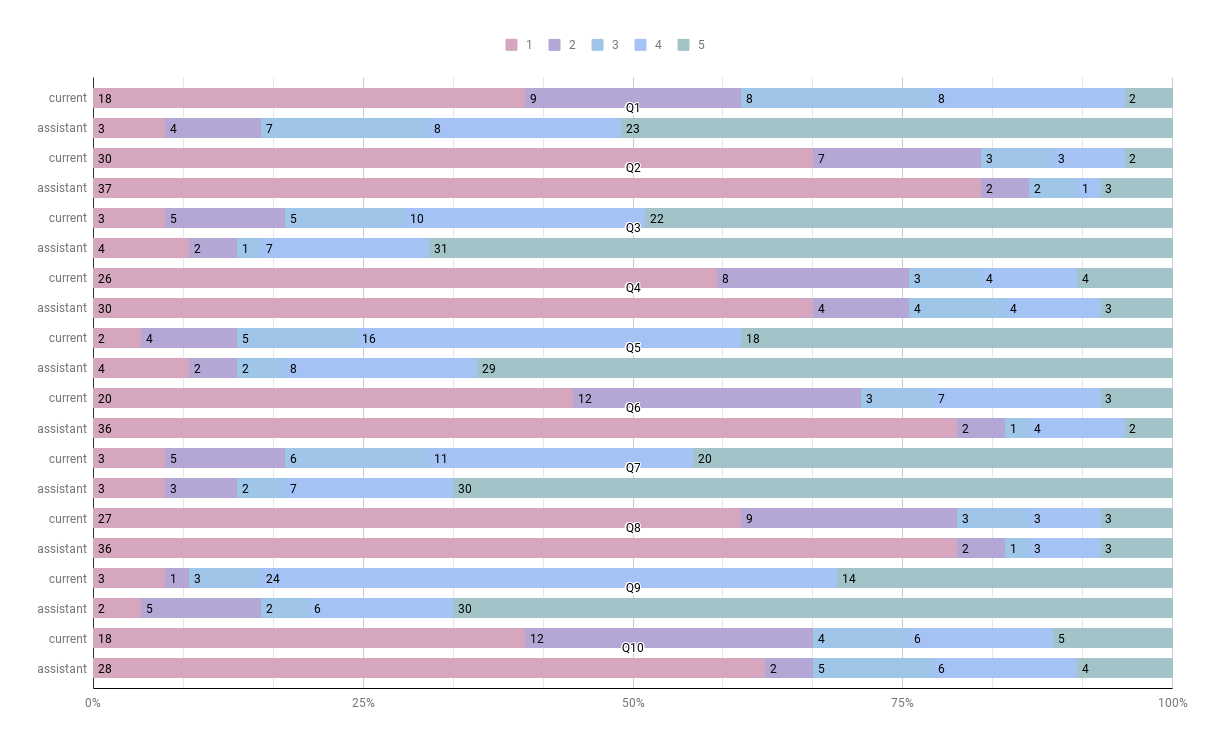
\includegraphics[width=\columnwidth]{images/fig109}
\caption{Results of SUS scores between {\it current} (Clinician-Only) and {\it assistant} (Clinician-AI) conditions. The bars represent the mean score for each question, {\it i.e.}, ranging from 1 = ``Strongly disagree'' to 5 = ``Strongly agree'' of the scale. The SUS questionnaire consists of ten questions (Q1 to Q10), displaying the results of each question in two rows of {\it current} and {\it assistant} conditions. A visual representation provides information on participants' responses to each question, allowing for comparative analysis.}
\label{fig:fig109}
\end{figure}
%%%%%%%%%%%%%%%%%%%%%%%%%%%%%%%%%%%%%%%%%%%%%%%%%%%

\textcolor{revised}{The \ac{NASA-TLX} questionnaire was utilized to assess perceived workload, enabling an analysis of cognitive load changes across different conditions.
A one-way \ac{ANOVA} test was conducted for this purpose, revealing significant differences in workload between the Clinician-AI and Clinician-Only conditions.
The test yielded an F(3, 41) = 3.274, indicating statistical significance (p = 0.03 $<$ 0.05).
These results highlight the Clinician-AI condition's effectiveness in reducing perceived workload compared to the Clinician-Only condition ($\sim$48\%).
Regarding specific values, the Clinician-AI condition resulted in a lower perceived workload (M = 5.729, SD = 0.819) than the Clinician-Only condition (M = 11.99, SD = 5.556).
Cohen's effect size was calculated with {\it f} = 0.081, suggesting a small effect, while $\eta^{2}$ = 0.0066, explaining approximately 0.7\% of the variance in workload between conditions.}

\textcolor{revised}{The Clinician-AI condition resulted in lower perceived mental and physical demands (Section~\ref{sec:app003004003} of Appendix~\ref{chap:app003}).
However, its performance was perceived less favorably (Section~\ref{sec:app003004004} of Appendix~\ref{chap:app003}), possibly due to more visualization modalities and a larger amount of information, including explanations.
Nonetheless, these results show the \ac{AI} assistant's role in reducing cognitive and physiological strains in medical decision-making.
Clinicians noted enhanced efficiency and performance, highlighting the \ac{AI} system's effectiveness in easing cognitive burden and improving workflow productivity.}

In assessing the usefulness of the \ac{AI} assistance, structured {\it post-task} interviews and comprehensive {\it open-ended} queries were conducted, as referenced in Section~\ref{sec:app003005002} of Appendix~\ref{chap:app003}.
This approach was specifically chosen to objectively capture clinicians' insights regarding the system's efficacy and integration into their regular practice.
Analysis of these qualitative inputs revealed that the majority of clinicians (41/45) have actively incorporated the \ac{AI} algorithm into their daily clinical routines.
Moreover, clinicians reported noticeable enhancements in their operational efficiency and workflow optimization (28/45), attributable to the \ac{AI} tool.
These results not only demonstrate a robust adoption of the \ac{AI} assistant but also suggest its significant impact in augmenting clinical performance and workflow management.

\vspace{2.50mm}

\noindent
Comments highlighted the valuable role of the assistant in enhancing diagnostic accuracy, reducing workload, and enabling new quantitative information to be added to reports:

\vspace{2.50mm}

\noindent
``The system [{\it BreastScreening-AI} assistant] will be a great asset for us.'' (C6)

\vspace{2.50mm}


Indeed, clinicians (33/45) expressed positive views on the system's ability to improve diagnostic accuracy, provide timely and relevant information, and facilitate more informed decision-making.
The results indicated that design interventions played a crucial role in enhancing the perceived usefulness of the system.
Integrating \ac{AI} technologies in radiology was seen as a promising approach to augment clinical practices and enable better patient care.

In conclusion, integrating an intelligent agent into the clinical workflow was well-received by clinicians.
This success is due to strategic design interventions, informed by a human-centered approach, providing substantial insights for our {\bf RQ5.1}.
The \ac{AI} assistant received favorable feedback from clinicians, resulting in higher levels of acceptance, satisfaction, and usability when compared to the Clinician-Only scenario.
Notably, the \ac{AI} assistant effectively reduced workload, while also being perceived as valuable in enhancing diagnostic accuracy and improving overall clinical practices.
These findings underscore the potential of \ac{AI}-assisted techniques in optimizing the radiology workflow and empowering clinicians to make well-informed decisions.

The positive reception and acceptance of the \ac{AI} assistant by clinicians highlight the importance of integrating intelligent agents into medical practices, paving the way for continued advancements in healthcare delivery.
As \ac{AI} technologies continue to evolve and improve, it is crucial to foster ongoing collaboration between clinicians, researchers, and technology developers to ensure the responsible and ethical integration of \ac{AI} in radiology and beyond.
By harnessing the full potential of \ac{AI}-assisted techniques, we can aspire to achieve higher levels of precision, productivity, and quality in healthcare, ultimately benefitting both medical professionals and the patients they serve.

\subsection{RQ5.2: Understanding and Trust Enhancement}
\label{sec:chap005006002}

To address the research question {\bf RQ5.2}, we investigated how design techniques can improve clinicians' understanding and trust of the \ac{AI} recommendations by considering the explainability power of the system (Figure~\ref{fig:fig111}).
We measured clinicians' understanding, while assessing clinicians' trust across the Model of Trust~\cite{CALISTO2021102607} using the \ac{DOTS} questionnaire (Section~\ref{sec:app003004007} of Appendix~\ref{chap:app003}) for this purpose.
In addition, we collected feedback (Section~\ref{sec:app003005002} of Appendix~\ref{chap:app003}) on the explainability functionalities of the system through qualitative interviews so that we can understand how well the system provides explanations for its \ac{AI} recommendations.

%%%%%%%%%%%%%%%%%%%%%%%%%%%%%%%%%%%%%%%%%%%%%%%%%%%
\begin{figure}[htbp]
\centering
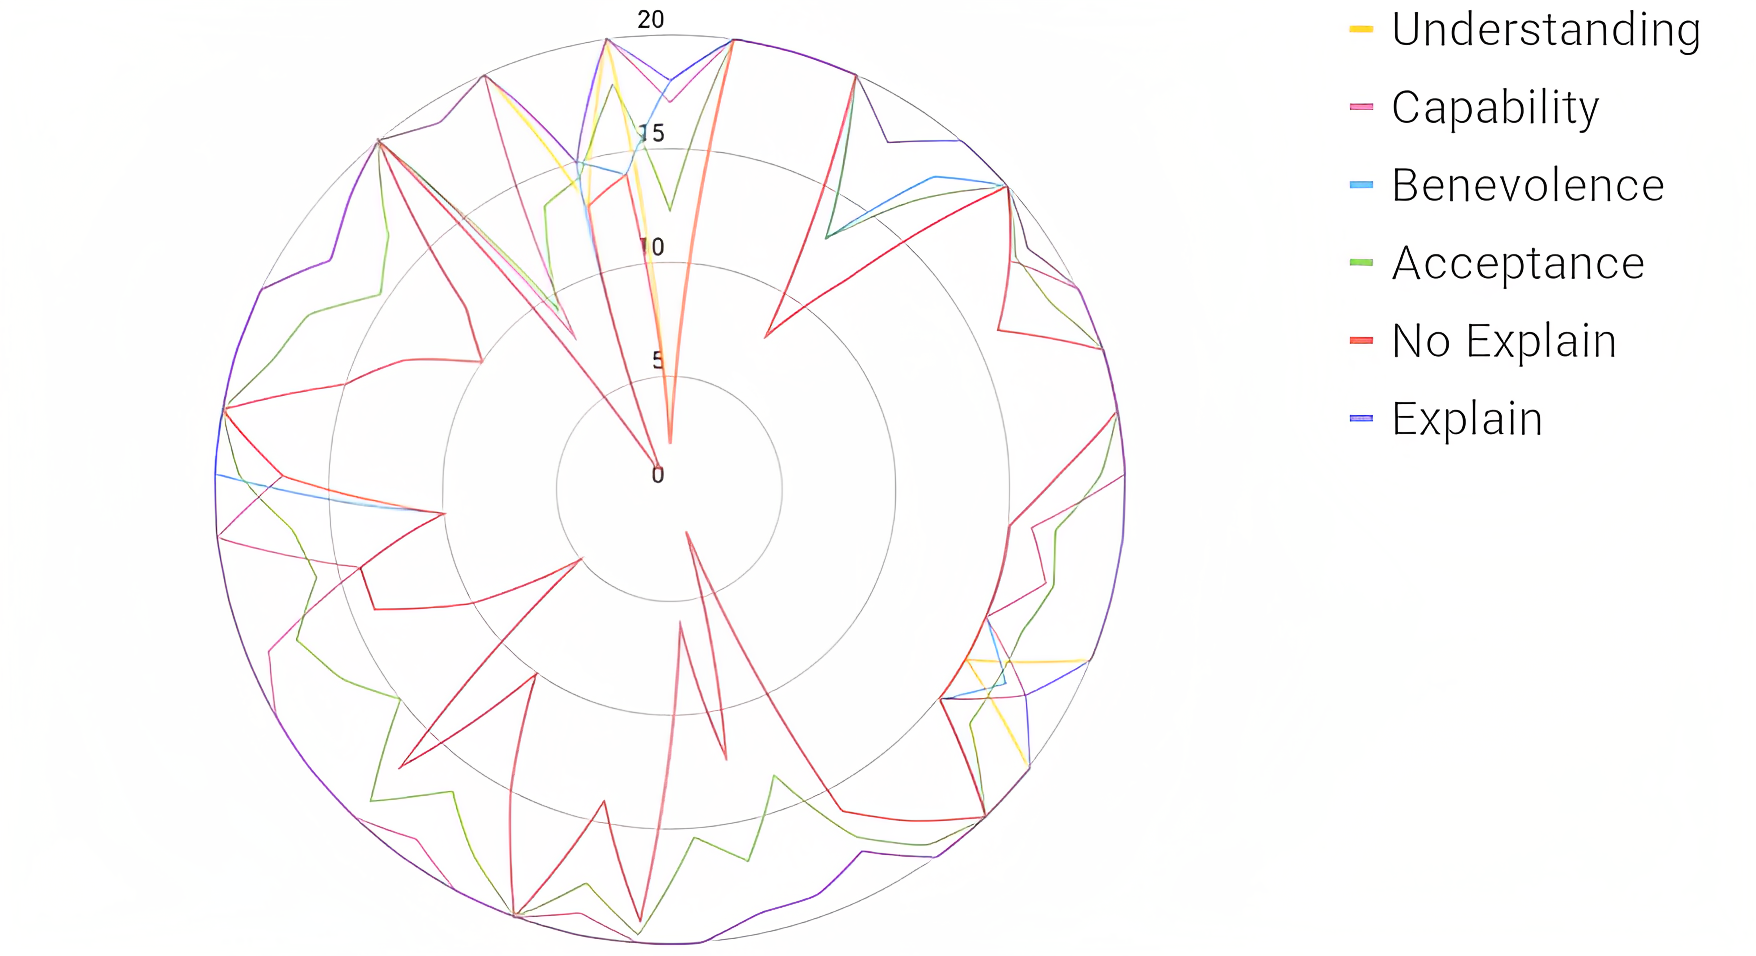
\includegraphics[width=\columnwidth]{images/fig111}
\caption{Results of DOTS and acceptance scores for the {\it assistant} (Clinician-AI) conditions. Each question is ranging from 1 = ``Strongly disagree'' to 20 = ``Strongly agree'' of the scale. The figure provides a visual representation of the participant's responses to perceived {\it Understanding}, {\it Capability}, and {\it Benevolence} of the DOTS scores. Additionally, we measured perceived overall {\it Acceptance} on the assistant, as well as differences in acceptance when clinicians do not ask ({\it No Explain}) or ask ({\it Explain}) for explanations.}
\label{fig:fig111}
\end{figure}
%%%%%%%%%%%%%%%%%%%%%%%%%%%%%%%%%%%%%%%%%%%%%%%%%%%

In this study, we employed a visual technique utilizing heatmaps to highlight regions of severity in the recommendations of the \ac{AI} system.
The heatmap information visualization effectively conveyed the severity of lesions, with hotter colors (Figure~\ref{fig:fig032}) indicating higher severity.
Results from the \ac{DOTS} questionnaire (Figure~\ref{fig:fig111}) indicated that 98\% of the clinicians comprehended the reasoning behind the system, demonstrating a high level of understanding.
Specifically, clinicians exhibited greater levels of perceived understanding when actively engaging with the assistant by pressing the {\it Explain} button (M = 19.7, SD = 2.92) compared to refraining from pressing it (M = 10, SD = 7).
This highlights the role of more granular explanations~\cite{10.1145/3544548.3580945}, enhancing clinicians' understanding of \ac{AI}-assisted diagnostics.

A notable 93\% of clinicians conveyed confidence in the system's abilities, underscoring their trust in the \ac{AI} system's recommendations for precise patient diagnosis.
Through the introduction of {\it Accept} ({\it Re-6.1.}), {\it Reject} ({\it Re-6.3.}), and {\it Explain} ({\it Re-6.2.}) buttons (Figure~\ref{fig:fig040}), perceived benevolence (M = 14.67, SD = 5.24) was increased while providing control and flexibility of the final diagnosis.
After asking for an explanation, 76\% of the clinicians increased their agreement ({\it i.e.}, pressing the {\it Accept} button) with the final diagnostic.

Finally, 91\% accept and prefer the \ac{AI} setup (Figure~\ref{fig:fig111}).
Trust values in our assistant (M = 18.81, SD = 2.96) were significantly higher (p = 0.0003 $<$ 0.05) when compared to clinicians who did not press the {\it Explain} button (M = 12.43, SD = 3.21).
Bringing higher levels of acceptance to the \ac{AI} recommendations of the assistant when explaining the severity classification of lesions through heatmaps.
Additionally, there was no significant imbalance in prior frequency for using the {\it BreastScreening-AI} framework.

In conclusion, our study addressed the research question {\bf RQ5.2} by investigating how design techniques can enhance clinicians' understanding and trust in \ac{AI} recommendations, considering the explainability power of the system.
We employed various metrics and questionnaires to assess clinicians' understanding and trust.
Using heatmaps as a visual information technique effectively conveyed the severity of lesions, and clinicians exhibited a high level of understanding, comprehending the reasoning behind the system.
This resulted in higher levels of perceived understanding, where clinicians expressed increased trust in the system's capabilities.

The inclusion of control functionalities further increased perceived benevolence.
Moreover, clinicians preferred the \ac{AI} setup, indicating a positive acceptance of the \ac{AI} recommendations.
Our findings demonstrate that the explainability functionalities achieved through our design process enhance clinicians' understanding and trust in autonomous recommendations, promoting their acceptance and preference for the \ac{AI} setup.

\subsection{RQ5.3: Workflow Impact}
\label{sec:chap005006003}

In this section, we present the results obtained to answer research question {\bf RQ5.3}, which focuses on the impact of \ac{AI} assistance on the medical workflow, including accuracy (Section~\ref{sec:app003004009003} of Appendix~\ref{chap:app003}), time performance (Section~\ref{sec:app003004009}), and variability (Section~\ref{sec:app003004008}) in patient classification.
We begin by investigating the rates of \acp{FP} and \acp{FN} with and without \ac{AI} assistance.
Then, we examine the diagnostic time and breast severity concerning using \ac{AI} assistance.
Next, we delve into the clinical impact of \ac{AI} assistance, exploring the improvement in accuracy and time performance.
Lastly, we discuss the alterations in clinical workflows resulting from integrating \ac{AI} assistance.
By presenting these results, we aim to provide a comprehensive understanding of the \ac{AI} assistance impact on the medical workflow.
The findings shed light on the benefits of \ac{AI} in healthcare settings, including enhanced accuracy, reduced diagnostic time, and improved consistency in patient classification.

\textcolor{revised}{In Table~\ref{tab:tab017}, a comparison of \ac{FP} and \ac{FN} rates was conducted between scenarios where clinicians worked alone and those where they were assisted by \ac{AI} (Section~\ref{sec:app003004009001} of Appendix~\ref{chap:app003}).
The findings revealed a notable decline in \acp{FP} when \ac{AI} was utilized, signifying an adaptation in the risk tolerance of radiologists.
In particular, the incidence of \acp{FP} fell from 39\% to 15\% \textcolor{revised}{{\it compound reduction}} with the aid of our intelligent agents, demonstrating a decreased tendency towards overestimating diagnoses.
This substantial 24\% \textcolor{revised}{{\it compound reduction}} in \acp{FP} underscores the effectiveness of \ac{AI} in refining the accuracy of patient classification and curtailing superfluous treatments~\cite{10.1001/jamainternmed.2014.981}.
Furthermore, there was a 19\% \textcolor{revised}{{\it compound reduction}} in \acp{FN} with \ac{AI} assistance, indicating a more measured approach to risk.
This suggests that \ac{AI}'s application mitigates the issue of overdiagnosis and bolsters the identification and categorization of breast anomalies, thereby ensuring more precise diagnoses and minimizing the likelihood of overlooking critical conditions.
These insights highlight the significant role of \ac{AI} in augmenting the precision of patient classification and judicious risk management in clinical decision-making processes.}

%%%%%%%%%%%%%%%%%%%%%%%%%%%%%%%%%%%%%%%%%%%%%%%%%%%
% Please add the following required packages to your document preamble:
% \usepackage{multirow}
% \usepackage{graphicx}
\begin{table}[]
\resizebox{\textwidth}{!}{%
\begin{tabular}{|c|cc|cccc|cccc|}
\hline
\multirow{3}{*}{Groups} &
  \multicolumn{2}{c|}{Low} &
  \multicolumn{4}{c|}{Medium} &
  \multicolumn{4}{c|}{High} \\ \cline{2-11} 
 &
  \multicolumn{1}{c|}{Cli.-Only} &
  Cli.-AI &
  \multicolumn{1}{c|}{Cli.-Only} &
  \multicolumn{1}{c|}{Cli.-AI} &
  \multicolumn{1}{c|}{Cli.-Only} &
  Cli.-AI &
  \multicolumn{1}{c|}{Cli.-Only} &
  \multicolumn{1}{c|}{Cli.-AI} &
  \multicolumn{1}{c|}{Cli.-Only} &
  Cli.-AI \\ \cline{2-11} 
 &
  \multicolumn{1}{c|}{FPs} &
  FPs &
  \multicolumn{1}{c|}{FPs} &
  \multicolumn{1}{c|}{FPs} &
  \multicolumn{1}{c|}{FNs} &
  FNs &
  \multicolumn{1}{c|}{FPs} &
  \multicolumn{1}{c|}{FPs} &
  \multicolumn{1}{c|}{FNs} &
  FNs \\ \hline
Intern &
  \multicolumn{1}{c|}{0.58} &
  0.42 &
  \multicolumn{1}{c|}{0.75} &
  \multicolumn{1}{c|}{0.08} &
  \multicolumn{1}{c|}{0.08} &
  0.08 &
  \multicolumn{1}{c|}{0.33} &
  \multicolumn{1}{c|}{0.08} &
  \multicolumn{1}{c|}{0.17} &
  0.08 \\ \hline
Junior &
  \multicolumn{1}{c|}{0.63} &
  0.13 &
  \multicolumn{1}{c|}{0.38} &
  \multicolumn{1}{c|}{0.13} &
  \multicolumn{1}{c|}{0.13} &
  0.13 &
  \multicolumn{1}{c|}{0.50} &
  \multicolumn{1}{c|}{0.25} &
  \multicolumn{1}{c|}{0.13} &
  0.13 \\ \hline
Middle &
  \multicolumn{1}{c|}{0.43} &
  0.21 &
  \multicolumn{1}{c|}{0.79} &
  \multicolumn{1}{c|}{0.21} &
  \multicolumn{1}{c|}{0.07} &
  0.07 &
  \multicolumn{1}{c|}{0.21} &
  \multicolumn{1}{c|}{0.07} &
  \multicolumn{1}{c|}{0.14} &
  0.07 \\ \hline
Senior &
  \multicolumn{1}{c|}{0.45} &
  0.36 &
  \multicolumn{1}{c|}{0.73} &
  \multicolumn{1}{c|}{0.09} &
  \multicolumn{1}{c|}{0.09} &
  0.18 &
  \multicolumn{1}{c|}{0.09} &
  \multicolumn{1}{c|}{0.09} &
  \multicolumn{1}{c|}{0.09} &
  0.09 \\ \hline
\end{tabular}%
}
\caption{Comparison of FP and FN rates between the Clinician-Only ({\it Cli.-Only}) setup and the Clinician-AI ({\it Cli-AI}) setup, categorized by severity levels ({\it i.e.}, {\it Low}, {\it Medium}, and {\it High}), across different levels of medical professional experience ({\it i.e.}, {\it Inter}, {\it Junior}, {\it Middle}, and {\it Senior} levels) of clinicians. The table presents the rates of FPs and FNs, providing insights into the performance of the two setups across severity categories and clinician experience levels. For {\it Low} severities (BI-RADS = 1), we only provide FPs rates since we did not consider lower (BI-RADS = 0) rates.}
\label{tab:tab017}
\end{table}
%%%%%%%%%%%%%%%%%%%%%%%%%%%%%%%%%%%%%%%%%%%%%%%%%%%

From a dataset of 289 patients, we analyzed our results to explore the relationship between diagnostic time and breast severity (Section~\ref{sec:app003004005} of Appendix~\ref{chap:app003}).
Our findings revealed notable differences in diagnostic time across different severity levels.
For patients with low severity ({\bf P1}), the average diagnostic time in the Clinician-Only condition was 146 seconds (SD = 86.17), whereas the Clinician-AI condition showed a shorter average of 89 seconds (SD = 74.13).
Similarly, for patients with medium severity ({\bf P2}), the Clinician-Only condition had an average diagnostic time of 78 seconds (SD = 48.05), while the Clinician-AI condition exhibited a slightly lower average of 77 seconds (SD = 96.80).
Notably, patients with high severity ({\bf P3}) experienced a longer average diagnostic time of 116 seconds (SD = 65.70) in the Clinician-Only condition compared to the Clinician-AI condition, which had an average of 64 seconds (SD = 86.94).
\textcolor{revised}{Moreover, the one-way \ac{ANOVA} test, resulting in F(1, 44) = 11.31 with a p-value of 0.005 (p $<$ 0.05), indicates a significant influence of clinical experience on the time taken to diagnose cases of varying severity.
This result underscores that \ac{AI} assistance notably decreases diagnostic time across different severity levels.
The analysis further reveals that the clinicians' level of medical experience affects the time efficiency in decision-making.}

The introduction of \ac{AI} assistance positively influenced both inter-variability and intra-variability agreement (Section~\ref{sec:app003004008} of Appendix~\ref{chap:app003}) among clinicians during patient classification.
With \ac{AI} assistance, there were significant reductions in variability.
Regarding inter-variability, the \ac{CV} decreased from 57.69\% to 46.69\% for patients with low severity, demonstrating improved agreement and consistency among clinicians.
For patients with a medium severity, inter-variability improved by 3.28\%, while the most notable improvement of 34.10\% was observed for patients with high severity.
Intra-variability also decreased within specific clinician groups, including interns, juniors, middles, and seniors, with reductions ranging from 6.65\% to 23.66\%.
These findings indicate that \ac{AI} assistance enhances inter-variability agreement and reduces variability within clinician groups based on their medical professional experience.

Overall, \ac{AI} assistance promotes more reliable and consistent patient classification outcomes, improving diagnostic decisions.
Therefore, clinicians benefit from improved agreement and enhanced diagnosis consistency, improving patient care.
The results of this study demonstrate the positive impact of \ac{AI} assistance on the medical workflow.
The utilization of \ac{AI} assistance significantly improves accuracy in patient classification, reduces the time required for various tasks, and enhances inter-rater agreement.
These findings support the integration of \ac{AI} technologies in healthcare settings, emphasizing their potential to enhance efficiency, accuracy, and consistency in decision-making during breast cancer diagnosis.

\subsection{Summary}
\label{sec:chap005006004}

Here, we encapsulate the main findings of our study.
These results summarize each facet of our investigation, elucidating the impact of \ac{AI} medical assistance and the advantages of employing a human-centered design approach.
By analyzing these crucial aspects, we aim to elucidate the effects of design interventions on clinicians' experiences and perceptions.
The analysis of satisfaction and acceptance encompasses usability, workload, and usefulness, while understanding and trust enhancement focuses on clinicians' comprehension and confidence in \ac{AI} recommendations.
Finally, the investigation of workflow impact delves into accuracy, diagnostic time, and variability in patient classification.

\textcolor{revised}{In addressing satisfaction and acceptance ({\bf RQ5.1}), our study found that implementing \ac{AI} assistance with targeted design interventions markedly enhanced clinicians' satisfaction and acceptance in radiology settings.
According to the \ac{SUS} questionnaire, the \ac{AI}-assisted condition achieved a 69\% higher agreement rate, reflecting a 91\% increase in perceived usefulness of \ac{AI}-assisted techniques over the Clinician-Only approach.
Notably, 82\% of clinicians affirmed the system's usability, ease of use, and effective integration into their workflow.
The \ac{NASA-TLX} scores confirm a notable decrease in cognitive workload ($\sim$48\%) with \ac{AI} assistance.
Post-task feedback indicates clinicians appreciate the \ac{AI} system's clear insights for better diagnostics.
These findings emphasize user-centered design's importance in improving clinician satisfaction with \ac{AI} tools in radiology, leading to more efficient, effective care.}

Regarding understanding and trust enhancement ({\bf RQ5.2}), our study revealed that design techniques could improve clinicians' understanding and trust in \ac{AI} recommendations.
About 85\% of clinicians exhibited a high level of understanding and trust in the system's capabilities.
Including explainability functionalities, such as heatmaps and control functionalities, increased perceived understanding and benevolence, respectively.
Specifically, 62\% of clinicians positively accepted the \ac{AI} setup, indicating their preference for \ac{AI} recommendations.
These findings emphasize the importance of explainability in enhancing clinicians' understanding and trust in \ac{AI} assistance.

Regarding workflow impact ({\bf RQ5.3}), our results demonstrated that \ac{AI} assistance positively impacts the medical workflow in radiology.
Using \ac{AI} assistance reduced the medical error percentile by 15\% for \acp{FP} and 2\% for \acp{FN}, improving patient classification accuracy.
Diagnostic time was significantly reduced by an average of 50 seconds per patient across different severity levels, indicating enhanced efficiency.
Furthermore, \ac{AI} assistance improved clinician agreement and consistency, reducing inter-variability and intra-variability.
These findings highlight the potential of \ac{AI} assistance to optimize the medical workflow, leading to better patient care and treatment decisions.

\textcolor{revised}{In conclusion, our research explored clinician interactions with \ac{AI} assistance in radiology, focusing on satisfaction, acceptance, understanding, trust, and workflow enhancement.
A human-centered approach facilitated the effective integration of intelligent agents into clinical practice, enhancing user satisfaction and trust in \ac{AI} recommendations.
This integration optimized the medical workflow, improving diagnostic accuracy, reducing time, and increasing consistency, thereby enhancing decision-making reliability and clinician efficiency.}

\section{Discussion}
\label{sec:chap005007}

In this section, we summarize the study's findings, discuss their implications, and identify areas for further investigation.
We contextualize our findings within the existing research landscape, compare them with previous studies, and highlight their practical significance.
We also acknowledge the limitations of the study and propose future directions.
Further discussion are provided in Section~\ref{sec:app003005} of Appendix~\ref{chap:app003}.

\subsection{Findings}
\label{sec:chap005007001}

Interpreting the results in light of existing literature~\cite{10.1145/3411764.3445432} and theoretical frameworks~\cite{10.1145/3311957.3361858} allows us to contextualize our findings within the broader research landscape and theoretical understanding of the topic.
It provides an opportunity to compare and contrast our results with previous studies~\cite{CALISTO2022102285, CALISTO2021102607}, identify areas of alignment or divergence, and discuss the practical significance of our findings.
Additionally, addressing the study's limitations and suggesting areas for further investigation helps to acknowledge the scope of our work and identify avenues for future research (Section~\ref{sec:app003005004}).

Our study examined various elements of clinician interactions with \ac{AI} assistance in radiology.
Using a human-centered approach and design interventions, we successfully integrated intelligent agents into clinical settings.
The research revealed significant results and new insights into the practical advantages of medical \ac{AI} assistance.

Starting with satisfaction and acceptance ({\bf RQ5.1}), our findings highlight the crucial role of integrating \ac{HCI} principles into the design process of \ac{AI} systems.
Through these design interventions, we notably enhanced clinicians' satisfaction and acceptance of the final solution.
Our results align with prior studies~\cite{10.1145/3411764.3445432}, emphasizing the benefits of design interventions and reinforcing the essential role of \ac{HCI} principles in promoting positive \ac{AI} system engagement.
The higher agreement percentages and positive perceptions of usability, ease of use, and workflow integration highlight the effectiveness of design interventions in enhancing clinicians' satisfaction and acceptance of \ac{AI} assistance (Section~\ref{sec:app003005002} of Appendix~\ref{chap:app003}).
By incorporating \ac{HCI} principles like \ac{UCD} and usability testing in \ac{AI} system development, we ensure design interventions align with clinicians' needs, enhancing user satisfaction and acceptance.

In terms of understanding and trust enhancement ({\bf RQ5.2}), our study demonstrated the effectiveness of design techniques in improving clinicians' understanding and trust in \ac{AI} recommendations.
The results align with theoretical frameworks~\cite{10.1145/3311957.3361858} that emphasize the significance of explainability and transparency in fostering trust in \ac{AI} systems.
By incorporating explainability functionalities, such as heatmaps and control functionalities, we observed improvements in clinicians' understanding and perceived benevolence of the \ac{AI} system.
These enhancements contributed to their acceptance and preference for \ac{AI} recommendations.
The findings highlight the importance of incorporating explainability features in \ac{AI} system design to promote understanding and trust among clinicians.

Regarding workflow impact ({\bf RQ5.3}), our results indicated that \ac{AI} assistance positively impacts the medical workflow in radiology (Section~\ref{sec:app003005001} of Appendix~\ref{chap:app003}).
The reduction in \acp{FP} and \acp{FN}, improved accuracy in patient classification, and reduced diagnostic time highlight the potential of \ac{AI} assistance to optimize the medical workflow and enhance patient care.
These findings align with previous studies demonstrating the benefits of \ac{AI} in improving diagnostic accuracy and efficiency in healthcare settings.
The enhanced inter-rater agreement and reduced variability further support the notion that \ac{AI} assistance promotes more consistent and reliable patient classification outcomes.

In this study, we explored how design interventions could guide us in developing an optimal solution for radiology (Section~\ref{sec:app003006}), thereby underscoring the pivotal role of \ac{HCI} principles in designing \ac{AI} systems.
Our findings reveal the transformative potential of design interventions in augmenting decision-making and boosting diagnostic efficiency.
The outcomes underscore the necessity of considering \ac{HCI} principles and optimizing workflow integration when introducing \ac{AI} systems into healthcare environments.
We advocate for embracing \ac{HCI} principles in the design process to develop \ac{AI} systems that cater more effectively to clinicians' needs, ultimately enhancing diagnostic performance.

\subsection{Design Implications}
\label{sec:chap005007002}

Our findings highlight the potential of \ac{AI} assistance to enhance clinicians' decision-making, efficiency, and patient care in radiology.
The effective execution of design interventions and \ac{HCI} principles is crucial for achieving optimal solutions, resulting in enhanced user satisfaction, acceptance, understanding, and trust.
Applying \ac{HCI} principles and strategic design interventions is vital for successful \ac{AI} incorporation in clinical practice.
Enhancing clinicians' satisfaction and acceptance enables more effective utilization of \ac{AI} technologies in healthcare settings.
Design techniques that promote understanding and trust in \ac{AI} recommendations empower clinicians to make informed decisions, leading to better patient care outcomes.
Workflow improvements, including reduced diagnostic time, increased accuracy, and enhanced consistency, have significant implications for clinical practice, potentially improving the efficiency and effectiveness of diagnoses.
Optimizing the medical workflow through \ac{AI} assistance ultimately improves patient outcomes and enhances the overall quality of healthcare delivery.

\vspace{1.00mm}

\noindent
Based on our findings, we propose the following design implications:

\vspace{0.05mm}

\begin{itemize}

\item \textbf{Workflow Understanding and Task-Specific Evaluations}:
Researchers should aim to develop \ac{AI} systems tailored to the specific characteristics of clinical workflows and the straightforward tasks of clinicians.
This understanding is essential for recognizing clinicians' requirements and designing intelligent agents that effectively support their decision-making processes.
When evaluating the performance of \ac{AI} systems, it is vital to consider the high-level workflow actions and diagnostic mechanisms to ensure that the evaluations are task agnostic and provide comprehensive insights.

\vspace{0.025mm}

\item \textbf{Concrete Evidence and Insights}:
Intelligent agents should provide clinicians with concrete empirical evidence and insights, highlighting the consequences or benefits of heeding or disregarding different types of \ac{AI} predictions to mitigate diagnostic errors.
This can help address model ambiguity and build trust in the \ac{AI} system.
Researchers can enhance clinicians' understanding of the system's capabilities and limitations by detailing the areas in the \ac{AI} reasoning where mistakes occur and the potential impact on patients.
Providing transparent explanations and granular insights will empower clinicians to make well-informed decisions based on the \ac{AI} outputs.

\vspace{0.025mm}

\item \textbf{Optimizing Precision and Recall with Uncertainty and Explanations}:
When designing \ac{AI} systems, consider optimizing precision and recall metrics while incorporating model uncertainty and explanations.
By optimizing precision and recall, designers can strike a balance between minimizing \acp{FP} and \acp{FN} in the \ac{AI} outputs.
Additionally, providing clinicians with explanations and insights into model uncertainty and misunderstandings can help them better interpret and utilize the \ac{AI} system's recommendations.
This approach ensures clinicians know potential misunderstandings and can make informed decisions based on the system's outputs.

\end{itemize}

% \vspace{0.05mm}

\textcolor{revised}{These design implications emphasize \ac{HCI} principles in developing \ac{AI} systems for radiology.
By deepening the understanding of clinical workflows, providing tangible evidence, and fine-tuning key metrics like precision and recall, they guide tailored \ac{AI} tool creation.
This is pivotal for successful \ac{AI} integration in clinical settings, as following discussed in our design recommendations (Section~\ref{sec:chap005007003}).
They highlight the significant contributions of the \ac{HCI} community in shaping transparent, user-friendly \ac{AI} systems supportive of clinicians' decision-making, promoting a collaborative human-\acs{AI} relationship.}

\subsection{Design Recommendations}
\label{sec:chap005007003}

\textcolor{revised}{In the context of optimizing workflow integration for \ac{AI} systems in clinical radiology, we propose targeted design recommendations.
These are grounded in \ac{HCI} principles and aim at fostering a cycle of continuous evaluation and improvement.
The focus is developing user-centric \ac{AI} systems tailored for radiology practice, enhancing healthcare quality and efficiency.}

\vspace{1.00mm}

\noindent
\textcolor{revised}{Reflecting on our research findings, we present the following specialized design recommendations for the integration of \ac{AI} assistance in radiology:}

\vspace{0.025mm}

\begin{enumerate}

\item \textcolor{revised}{\textbf{Healthcare Professional-Oriented Usability}:
Prioritize user-centered design principles by involving clinicians in all stages of usability testing.
Include iterative sessions where radiologists interact with \ac{AI} prototypes, giving feedback on interface, responsiveness, and tool integration.
The aim is to develop \ac{AI} systems that seamlessly fit into radiology workflows, addressing clinician needs and boosting satisfaction and acceptance.}

\vspace{0.025mm}

\item \textcolor{revised}{\textbf{Targeted Explainability and Transparency}:
Develop and integrate explainability features for radiological applications, including advanced visualization tools mapping \ac{AI} decisions onto images, and interactive controls for clinicians to query \ac{AI} outputs.
These features aim to enhance clinicians' understanding of \ac{AI} recommendations, fostering transparency and interpretability crucial for informed decision-making.}

\vspace{0.025mm}

\item \textcolor{revised}{\textbf{Workflow-Specific Integration and Enhancement}:
Design \ac{AI} systems attuned to radiology workflows, customizing tools to match typical diagnostic processes.
Optimize compatibility with existing solutions, enhance image processing speed, and improve efficiency to reduce diagnostic time, boosting clinical productivity and patient throughput.}

\vspace{0.05mm}

\item \textcolor{revised}{\textbf{Adaptive Design through Longitudinal Studies}:
Conduct longitudinal studies that involve continuous engagement with radiologists to gather in-depth feedback on the \ac{AI} system's performance in real-world clinical settings.
Use this feedback for iterative design adjustments, allowing the \ac{AI} system to evolve with changing clinical practices and user needs.
This approach guarantees the long-term effectiveness and clinical relevance of \ac{AI} systems in the ever-evolving field of radiology.}

\end{enumerate}

% \vspace{0.05mm}

\textcolor{revised}{Central to these design recommendations is the concept of \textit{healthcare professional-oriented usability}.
This involves designing \ac{AI} systems that are inherently user-friendly for radiologists, facilitating smoother technology interactions.
Additionally, \textit{targeted explainability and transparency} in \ac{AI} decision-making processes are crucial.
This aspect is further explored in Chapter~\ref{chap:chap006}, emphasizing the importance of clear and transparent \ac{AI}-clinician communication.
Moreover, \textit{workflow-specific integration and enhancement} are key, advocating for the seamless incorporation of \ac{AI} into existing clinical workflows, thus augmenting rather than disrupting medical practices.
Lastly, the principle of \textit{adaptive design through longitudinal studies} underscores the necessity of continually evolving \ac{AI} systems to align with the dynamic needs of radiology, informed by ongoing research and clinician feedback.
These guidelines collectively advocate for \ac{AI} tools that are technologically advanced but also relevant and user-friendly, aiming to transform healthcare into a more efficient, precise, and collaborative field.}

\textcolor{revised}{Our design recommendations are key to successfully integrating \ac{AI} in radiology, as detailed in Section~\ref{sec:app003005003} of Chapter~\ref{chap:app003}.
These guidelines aim to enhance user satisfaction, acceptance, understanding, trust, and workflow efficiency, making \ac{AI} intuitive and effective for healthcare professionals.
This approach not only improves \ac{AI}'s reliability in clinical settings but also ensures alignment with healthcare professionals' specific needs and workflows.
By focusing on patient care, these design recommendations aid in accurate diagnoses with personalized strategies and foster collaboration between \ac{AI} systems and medical practitioners (Chapter~\ref{chap:chap006}), addressing the unique challenges of radiology.}

\subsection{Limitations}
\label{sec:chap005007004}

While our study provides valuable insights, it is essential to acknowledge its limitations.
One limitation is the specific focus on radiology, which may limit the generalizability of the findings to other medical domains.
Future research should explore the applicability and effectiveness of design interventions in different medical domains to gain a more comprehensive understanding of the impact of \ac{AI} assistance.

Further investigations should also consider longitudinal studies to examine \ac{AI} assistance's long-term effects and sustainability in clinical practice.
Understanding the evolving dynamics of clinician-\ac{AI} interaction over time and capturing potential challenges or benefits that emerge in the real-world deployment of \ac{AI} assistance would provide valuable insights for successfully integrating \ac{AI} technologies into routine healthcare practice.
Additionally, it is crucial to continue exploring the ethical and social implications of \ac{AI} assistance in radiology and healthcare in general.
This includes examining the impact on the roles and responsibilities of healthcare professionals, trust and acceptance, privacy and security considerations, and the potential biases or disparities that may arise in using \ac{AI} algorithms.

\section{Conclusion}
\label{sec:chap005008}

Integrating \ac{AI} techniques into the clinical workflow, along with design interventions, presents promising opportunities in healthcare.
The effective execution of design interventions and applying \ac{HCI} principles are crucial for achieving optimal solutions, leading to enhanced user satisfaction, acceptance, understanding, and trust.
By interpreting our results in the context of existing literature and theoretical frameworks, we have gained valuable insights into the practical implications of \ac{AI} assistance in radiology, underscoring the significance of incorporating \ac{HCI} principles in designing \ac{AI} systems.
The consolidation of \ac{HCI} principles and strategic design interventions is vital for successfully integrating \ac{AI} into clinical practice, playing a crucial role in achieving optimal solutions and enhancing diagnostic performance.

When considering \ac{HCI} principles such as user-centered design and usability testing, designers can create \ac{AI} systems that effectively address clinicians' needs and preferences, leading to improved user satisfaction and acceptance.
Furthermore, the study demonstrates the effectiveness of design techniques in enhancing clinicians' understanding and trust in \ac{AI} recommendations.
Incorporating explainability functionalities, such as heatmap visualizations and control mechanisms, improve clinicians' understanding of the system's reasoning and fosters trust in \ac{AI} recommendations.
This finding aligns with theoretical frameworks emphasizing transparency and explainability in building trust in \ac{AI} systems.

The workflow impact of \ac{AI} assistance is also evident from the results.
The reduction in \acp{FP} and \acp{FN}, improved accuracy in patient classification, and reduced diagnostic time indicate the potential of \ac{AI} assistance to optimize the medical workflow and enhance patient care.
These findings align with previous research demonstrating the benefits of \ac{AI} in improving diagnostic accuracy and efficiency in healthcare settings.
To optimize workflow integration, ensuring the effective development and implementation of \ac{AI} systems in clinical settings, several design recommendations are proposed.
These recommendations emphasize the importance of usability, explainability, transparency, integration, and continuous evaluation.
By following these recommendations, designers can create user-centric \ac{AI} systems that enhance the overall quality of healthcare delivery.

It is essential to acknowledge the limitations of the study.
The specific focus on radiology may limit the generalizability of the findings to other medical domains.
Future research should explore the applicability and effectiveness of design interventions in different healthcare contexts.
Longitudinal studies are also needed to examine the long-term effects and sustainability of \ac{AI} assistance in clinical practice.

In conclusion, this study highlights the promising opportunities of integrating \ac{AI} techniques into the clinical workflow through design interventions, particularly in radiology.
Our results show that the effective execution of these interventions and applying \ac{HCI} principles are crucial for achieving optimal solutions.
By incorporating \ac{HCI} principles and optimizing workflow integration, \ac{AI} systems can support decision-making and enhance clinicians' efficiency.
The findings provide valuable insights for successfully integrating \ac{AI} technologies into routine healthcare practice.
% If Printing on DOUBLE SIDED pages, the second page should be white.
% Otherwise, comment the following command:
\cleardoublepage
%
% Chapter 6
% #############################################################################
% This is Chapter 6
% !TEX root = main.tex
% #############################################################################
% Change the Name of the Chapter i the following line
\fancychapter{Personalization \& Customization}
\clearpage
% The following line allows to ref this chapter
\label{chap:chap006}

\noindent
{\it This Chapter~\ref{chap:chap006} was published in one top (A* in 2023) conference:}

\vspace{0.5mm}

\begin{itemize}
\item {\bf Francisco Maria Calisto}, Jo\~{a}o Fernandes, Margarida Morais, Carlos Santiago, Jo\~{a}o M. Abrantes, Nuno J. Nunes, and Jacinto C. Nascimento. 2023. Assertiveness-based Agent Communication for a Personalized Medicine on Medical Imaging Diagnosis. Proceedings of the 2023 CHI Conference on Human Factors in Computing Systems (CHI '23), April 23--28, 2023, Hamburg, Germany. Association for Computing Machinery, New York, NY, USA, Article 13, 1–20. DOI: \href{https://doi.org/10.1145/3544548.3580682}{doi.org/10.1145/3544548.3580682}
\end{itemize}

Until now, this thesis explored the factors influencing the acceptance and adoption of \ac{AI} systems (Chapter~\ref{chap:chap004}), where we found enough evidence for the needs of different user groups.
Then, we delved into designing interventions (Chapter~\ref{chap:chap005}) to enhance the acceptance and integration of \ac{AI} systems in healthcare settings.
In this chapter, our focus shifts to understanding how \ac{AI} systems should communicate to address the specific needs and characteristics of different user groups~\cite{10.1145/3544548.3580682}, particularly considering the professional experience of the clinician.

\section{Motivation}
\label{sec:chap006001}

\ac{AI} systems, driven by \ac{DL} techniques, hold promise for various healthcare applications~\cite{CALISTO2022102285, Hannun2019, Ruamviboonsuk2019}.
However, these systems often fail to capture the variability among clinicians, such as interns, juniors, middles, and seniors~\cite{Uddin2019}.
Integrating technological advancements in the clinical workflow, such as \ac{AI} systems, can potentially advance personalized and precision medicine~\cite{HO2020497, Wetzstein2020}.
Consequently, understanding how \ac{AI} systems should communicate (Figure~\ref{fig:fig097}), considering the professional experience of the clinician (Section~\ref{sec:chap004006001} of Chapter~\ref{chap:chap004}), becomes a crucial design question~\cite{pacheco2019alignment}.

%%%%%%%%%%%%%%%%%%%%%%%%%%%%%%%%%%%%%%%%%%%%%%%%%%%
\begin{figure}[htpb]

\includegraphics[width=\textwidth]{fig097}
\caption[]{A sample of ``Non-Assertive'' ({\it e.g.}, suggesting ``it looks like'') {\it vs.} ``Assertive'' ({\it e.g.}, imposing ``must'') communications.}
\label{fig:fig097}
\end{figure}
%%%%%%%%%%%%%%%%%%%%%%%%%%%%%%%%%%%%%%%%%%%%%%%%%%%

This study explores the application of the BreastScreening-AI framework in two conditions: conventional and assertiveness-based agents~\cite{pacheco2019alignment, 10.1145/3311350.3347162}.
By serving as a second reader, the intelligent agents aim to enhance diagnostic performance, reduce \acp{FP} and \acp{FN} (Over-Diagnosis {\it vs} Under-Diagnosis), and improve the efficiency and efficacy of the clinical workflow~\cite{CALISTO2022102285, 10.1145/3311350.3347162}.
While much research has focused on improving the accuracy of \ac{AI} algorithms, there is a necessity to address the adoption (Chapter~\ref{chap:chap004}) and usability (Chapter~\ref{chap:chap005}) concerns of interactive assistance techniques.
This study sheds light on clinicians' needs, practices, and attitudes toward \ac{AI}-powered assistance, emphasizing the importance of personalized communication and explanations to foster trust and acceptance of \ac{AI} systems~\cite{10.1145/3491102.3502104, CALISTO2021102607}.

Through a within-subject study involving 52 clinicians, our research examines the interaction between conventional and assertiveness-based agents in diagnosing a dataset of 289 patients~\cite{PELAU2021106855}.
The assertiveness-based agent utilizes different communication tones while providing human-interpretable clinical arguments to explain the \ac{AI} algorithms' diagnostic outputs~\cite{10.1145/3544548.3580682}.
This integration of \ac{DL} methods into communication theories allows us to explore the impact of assertiveness-based \ac{AI} mediation on clinicians with varying expertise levels (Section~\ref{sec:app005001} of Appendix~\ref{chap:app005}), specifically addressing critical medical decision-making scenarios~\cite{Aldoj2020}.
The findings from our study contribute to computational interaction approaches (Section~\ref{sec:app005017}), providing valuable insights into the design of interactive systems underpinned by computational principles for the \ac{HCI} community, particularly in high-stakes domains.

\vspace{1.50mm}

\noindent
The main contributions of this work are summarized as follows (detailed in Section~\ref{sec:app005002} of Appendix~\ref{chap:app005}):

\vspace{0.05mm}

\begin{enumerate}
\item Our novel approach customizes \ac{AI}-assisted medical reasoning, demonstrating the positive impact of assertiveness-based communication on clinical workflows.
\item We show that explaining \ac{AI} outputs improve medical efficiency, but its impact depends on the communication tone of the clinical arguments.
\item Our results show that assertiveness-based agents increase the utility of clinical information and user trust in \ac{AI} recommendations without compromising diagnostic performance.
\item We offer design considerations to adapt communication in \ac{AI}-assisted reasoning based on medical expertise levels, paving the way for future implementations of personalized intelligent agents.
\end{enumerate}

\vspace{0.50mm}

The following sections outline related works on the issues of guiding the \ac{HAII} topic, assisting clinical decision-making, going through some examples of \acp{CDSSe} present in the literature~\cite{NAISEH2023102941, 10.1145/3531146.3533193}, and ending on the effects of \ac{AI} communication.
We then introduce the design of our {\it Assertiveness-based BreastScreening-AI} assistant, followed by our research questions, hypotheses, and methods.
Last, we report our quantitative and qualitative findings, concluding with a discussion of design considerations.

\section{Related Work}
\label{sec:chap006002}

Medical imaging systems enable end-users to diagnose various modalities, including \ac{MG}, \ac{US}, and \ac{MRI}, through seamless data retrieval~\cite{10.1145/3544548.3580682}.
Integrating these modalities presents opportunities for quantitative imaging and diagnoses, necessitating specialized data handling, post-processing, and visualization methods~\cite{Igarashi:2016:IVS:2984511.2984537}.
In the clinical domain, medical imaging tools aid experts in making better decisions, such as identifying cancer prognostics from multi-modal data~\cite{10.1145/3399715.3399744}.
This chapter focuses on understanding different aspects and expectations of a \ac{CDSSe} integrated into the radiology workflow (Section~\ref{sec:app005003}), highlighting the enhancement of medical imaging diagnosis through assertiveness-based interaction.

In the context of \ac{HAII}, intelligent agents must go beyond providing results alone and consider user behaviors during decision-making~\cite{10.1145/3313831.3376807}.
In Section~\ref{sec:app005003001} of Appendix~\ref{chap:app005}, we delve deeper into this \ac{HAII} literature.
Additionally, we explore the interdisciplinary topic of \ac{XAI}, which intersects cognitive psychology, learnability, and context awareness within the field of \ac{HCI}~\cite{doi:10.1073/pnas.1618211113}.
Learnability, an essential aspect of usability, encompasses various aspects such as hints, guidance, and visualizations when designing \ac{XAI} systems\cite{10.1145/3173574.3174156}.
Furthermore, explainable context awareness simplifies context representation, providing users with information about the obtained data and system actions~\cite{10.1145/3313831.3376545}.

\ac{HAII} incorporates human feedback in model training to create better \ac{ML} models~\cite{10.1145/3290605.3300233, 10.1145/3132272.3134111, Kocielnik:2019:YAI:3290605.3300641, aha2017ai}, where we bring the topic focusing on personalized and customized \ac{AI} suggestions tailored to varying levels of medical expertise (Section~\ref{sec:app005003001}).
Researchers emphasize the importance of explaining \ac{AI} systems' reasoning to enhance \ac{HAII}, particularly in medical domains, where the interpretability of \ac{AI} predictions is crucial~\cite{10.1145/3411764.3445717, Rudin2022, Kawamleh2022}.
However, these approaches often fail to account for cognitive bias in decision-making, which varies among individuals with different levels of expertise and knowledge~\cite{https://doi.org/10.1111/nuf.12430, Seidel2021}.
Our work addresses these gaps by studying assertiveness-based communication in \ac{AI} systems, considering expertise levels to reduce cognitive bias.

The integration of \ac{AI} systems into clinical decision-making is a complex endeavor (Section~\ref{sec:app005003002} of Appendix~\ref{chap:app005}), as it presents challenges and unintended consequences~\cite{miller2019intrinsically}.
Critical decisions related to patient safety, clinician fatigue, and increased medical errors need to be carefully addressed~\cite{10.1093/jamia/ocab291, 10.1117/12.2613082, doi:10.1148/radiol.212631}.
Clinicians often find \ac{AI} systems challenging to use due to limited technical skills and a lack of customization to their behavioral aspects~\cite{CALISTO2022102922}.
Additionally, the understanding and communication of \ac{AI} outcomes to clinicians are hindered by poorly designed interfaces.
These interfaces often fail to consider the differences in clinician characteristics during decision-making, such as the varying reasoning approaches between novice and expert clinicians~\cite{Edgar2022}.

The lack of large-scale deployment of \ac{AI} systems in healthcare further complicates the understanding of how these systems are perceived and used in real-world settings~\cite{10.1145/3411764.3445432, SU202328, ZAPPATORE20231}.
While approaches such as \ac{iML}~\cite{10.1145/3544548.3580682}, \ac{HITL}~\cite{10.1145/3397481.3450668}, human-\ac{AI} symbiosis~\cite{JARRAHI2018577}, and human-\ac{AI} collaboration~\cite{10.1145/3411764.3445432} have been proposed in \ac{HCI}, they primarily focus on improving prediction accuracy, model efficiency, and interpretability without adequately considering the burden on healthcare professionals~\cite{10.1145/3555157, 10.1145/3209889.3209897}.
Existing studies on the perception and usage of \ac{AI} systems for clinical decision-making often overlook potential differences in behavioral reasoning.
Additionally, some approaches solely prioritize accurate algorithmic suggestions without accounting for the clinician's professional medical experience~\cite{10.1145/3491102.3502104}.
A more detailed literature review concerning these topics is further described in Section~\ref{sec:app005003002} of Appendix~\ref{chap:app005}.
Our research bridges the gaps between \ac{HCI} and \ac{AI} approaches, focusing on personalized and customized algorithmic suggestions based on varying levels of medical expertise.
These approaches empower clinicians, improves decision-making, and enhances patient care outcomes.

\acp{CDSSe} have greatly benefited from \ac{DL} algorithms~\cite{esteva2019guide} in various applications (Section~\ref{sec:app005003003} of Appendix~\ref{chap:app005}).
\ac{DL} systems have demonstrated their ability to detect patterns, make predictions, and assist clinicians in high-stakes decision-making processes~\cite{10.1145/3555157}, such as skin cancer diagnosis~\cite{esteva2017dermatologist}, cardiac \ac{MRI} segmentation~\cite{8759179}, and breast cancer detection~\cite{MAICAS2019101562}.
These models have shown exceptional performance in identifying meaningful patterns within medical data, sometimes surpassing human capabilities~\cite{10.1145/3544548.3580682}.
However, there is a need to adapt the communication tone of \acp{CDSSe} for personalized and customized medicine~\cite{MAICAS2019101562, CALISTO2022102285}, considering the unique behavioral characteristics and expertise levels of clinicians.
While \ac{DL}-based \acp{CDSSe} have shown promising results~\cite{mckinney2020international, Rajpurkar2022}, there are challenges in translating them from research and development environments to real clinical settings.

Utility to clinicians and logistical hurdles are common obstacles in clinical adoption~\cite{CALISTO2022102922}, and some systems have not effectively reduced clinician workload~\cite{KOHLI2018535} or improved diagnostic accuracy~\cite{KOHLI2018535}.
\ac{HCI} research in clinical environments has explored the evaluation of interactive \ac{DL} systems from a human-centered perspective~\cite{10.1145/3311957.3359433, 10.1145/3359206, 10.1145/3538882.3542790}.
Studies have investigated techniques to enhance diagnostic utility and user trust in \ac{DL} predictions, as well as identified important information for clinicians when integrating \ac{AI} assistants into routine practice~\cite{10.1145/3290605.3300234, 10.1145/3359206}.
However, these studies (Section~\ref{sec:app005003003}) have yet to consider the heterogeneous behavioral nature of decision-making among clinicians.

Trust plays a critical role in communication (Section~\ref{sec:app005003004} of Appendix~\ref{chap:app005}), especially in clinical environments where life-altering decisions are made~\cite{CALISTO2022102922}.
Positive motivational attribution and reducing ambiguity through trust~\cite{HOHENSTEIN2020106190} are key factors in successful collaboration between humans and \ac{AI}~\cite{10.1145/3479587, 10.1145/3334480.3375147, 10.1145/3334480.3382842}.
The impact of assertiveness-based \ac{AI} mediation on novice and expert clinicians is still not well understood~\cite{Lundberg2020}.
Understanding the effects of \ac{AI} communication is vital to avoid unforeseen clinical consequences.
Trust directly influences clinicians' perception of \ac{AI} outcomes and their attitudes, satisfaction, and performance evaluations~\cite{10.1145/3491102.3502104}.
Attribution theory and external cues shape clinicians' interpretation of information~\cite{10.1145/3544548.3580682}.
Our work introduces assertive communication theories into a deep learning system and clinical scenario, offering a novel approach to address these dynamics.

\section{Assertiveness-based System}
\label{sec:chap006003}

In this chapter, we explore how human-\ac{AI} interactions are affected by the ability of an \ac{AI} agent to not only incorporate granular patient information from the \ac{AI} outputs but also exploring how to adapt the communication tone ({\it i.e.}, more assertive or suggestive) depending on the medical experience ({\it i.e.}, novice or expert) of the clinician.
Specifically, we compare the \ac{AI} outputs (Figure~\ref{fig:fig096} and Figure~\ref{fig:fig112}) that explain to clinicians some clinical arguments with more granular information about the patient regarding the lesion details, to a conventional agent that only provides numeric estimates ({\it e.g.}, \ac{BI-RADS} and accuracy) of the classification.
Further details are described in Section~\ref{sec:app005004} of Appendix~\ref{chap:app005}.

%%%%%%%%%%%%%%%%%%%%%%%%%%%%%%%%%%%%%%%%%%%%%%%%%%%
\begin{figure}[htpb]
\centering
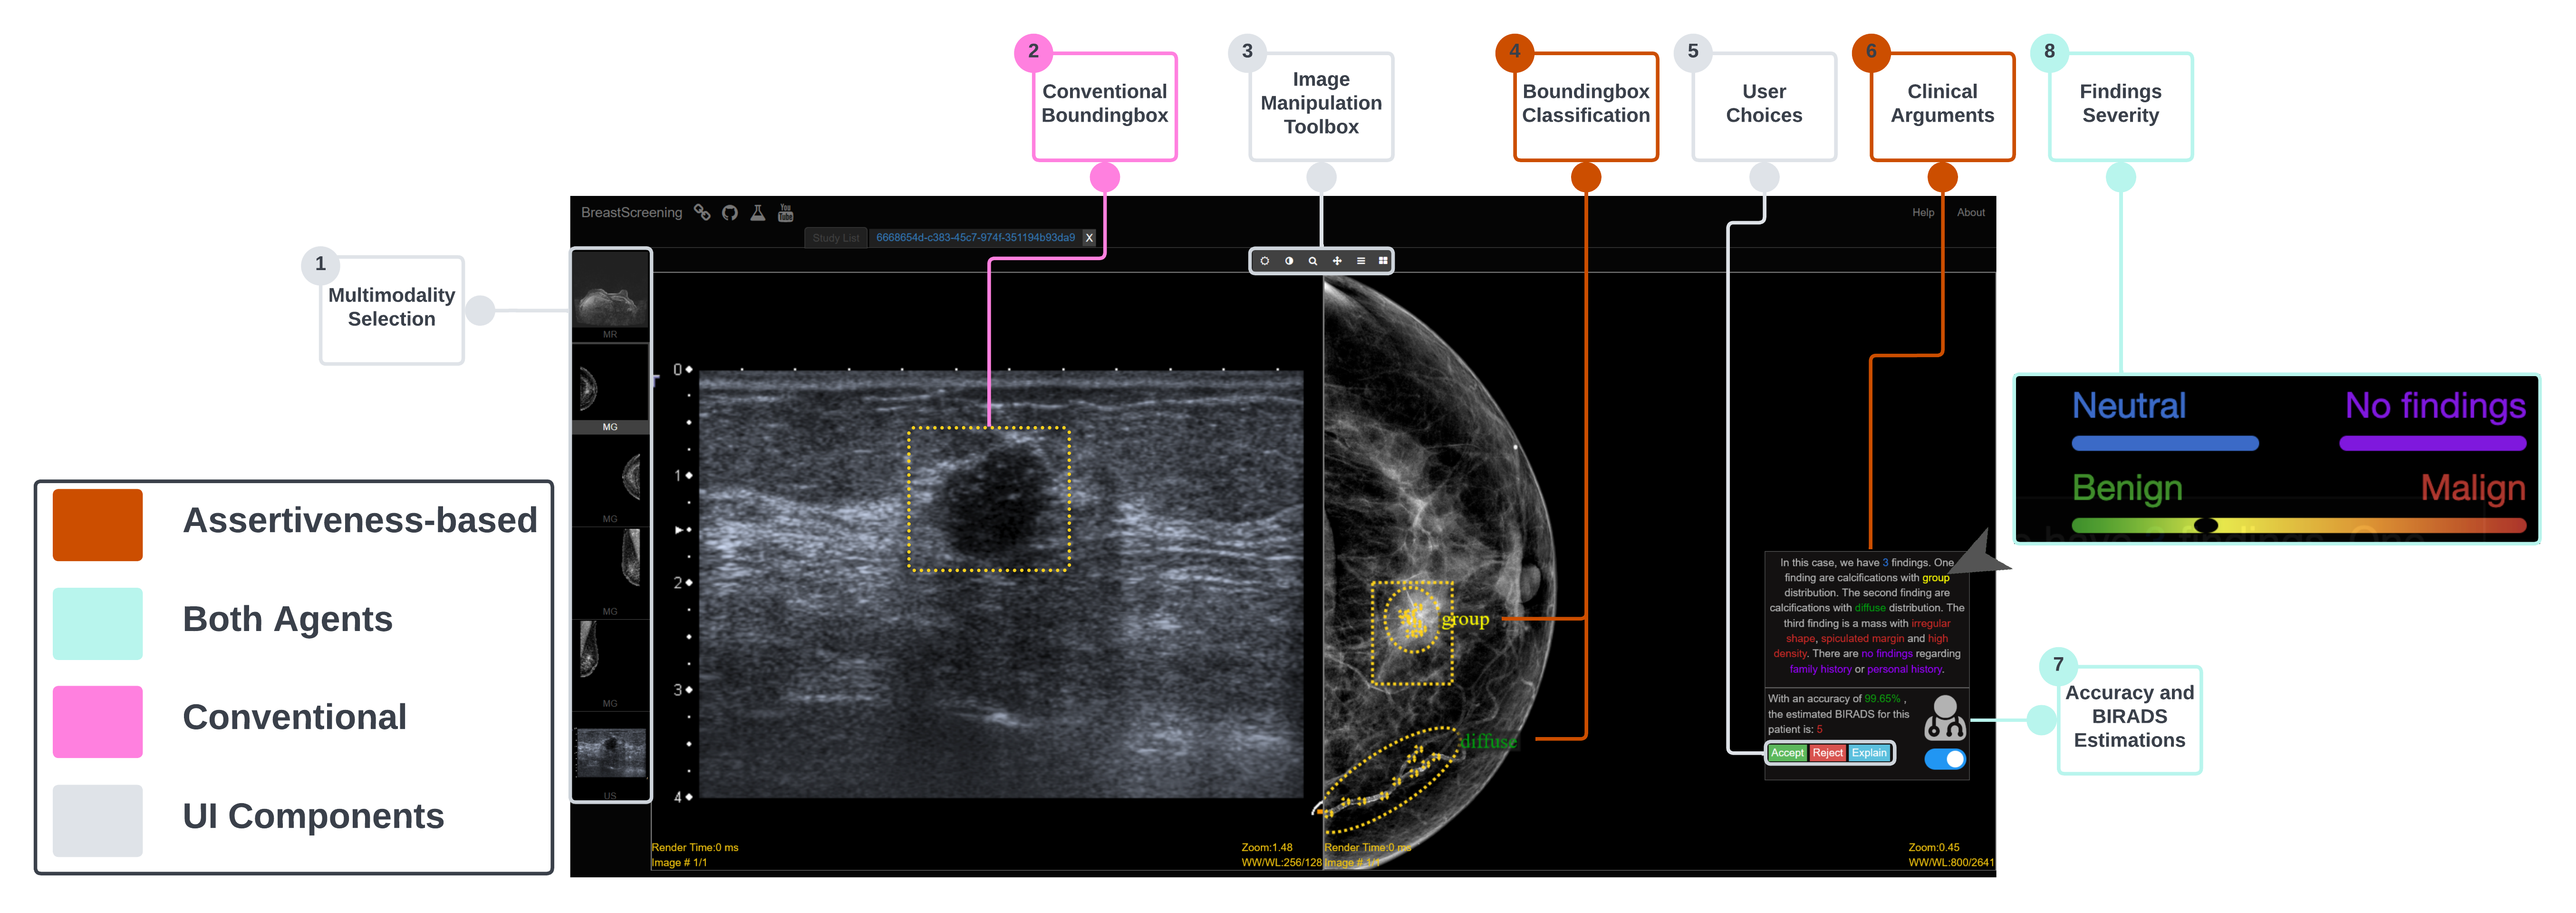
\includegraphics[width=1.000\textwidth]{fig096}
\caption[]{Interface for conventional and assertiveness-based AI agents for medical imaging analysis. Attributes are associated with numbers in each condition. AI agent provides severity information when hovering over variables. Colors range from benign (green) to malign (red). Number of findings displayed in neutral color (blue). Clinicians use purple color for family and personal history variables.}
\label{fig:fig096}
\end{figure}
%%%%%%%%%%%%%%%%%%%%%%%%%%%%%%%%%%%%%%%%%%%%%%%%%%%

Our assertiveness-based agent uses recommendations for classifying and segmenting:
(1) the number of detected findings;
(2) the patient severity of each breast and per medical imaging modality;
(3) a visual scale representing the benign or malign estimates;
(4) providing visualization of the sensitivity and specificity outcomes of the models; and
(5) with clinical arguments of the patient, such as pathological co-variables.
To compare the assertiveness-based agent to the conventional agent (Figure~\ref{fig:fig098}), we inform participants that the recommendations are generated by our \ac{AI} models so that they can also provide some feedback concerning the model performance.

Figure~\ref{fig:fig096} illustrates how the two \ac{AI} agents were integrated into an existing medical workflow for the classification of medical imaging data in support of breast cancer diagnosis.
Both agents are recommending classification and segmentation based on the DenseNet model~\cite{8721151} for \ac{MG} and \ac{US}, as well as based on the ResNet model~\cite{10.1145/3544548.3580682} for \ac{MRI}.
The two \ac{AI} agents provided the severity classification (Section~\ref{sec:app005009} of Appendix~\ref{chap:app005}) of the patient via \ac{BI-RADS}~\cite{SPAK2017179}, the accuracy of the model for that classification, and the segmentation of the lesion to explain the regions that derived from that classification.

\section{Research Questions \& Hypotheses}
\label{sec:chap006004}

The final purpose of our research is twofold.
Through assertiveness-based agents, we first aim to understand how personalized and customized communication could affect medical assessments in terms of the efficiency and efficacy of the clinical workflow.
Secondly, we aim to understand how clinicians perceive assertiveness-based agents differently.
Thus, our work addresses two primary research questions concerning the impact of assertiveness-based agents on efficiency and efficacy (RQ1), as well as the perception (RQ2) of clinicians.
We provide a more detailed view in Section~\ref{sec:app005005} of Chapter~\ref{chap:app005}.

\noindent
Specifically, we consider the following research questions and related hypotheses:

\vspace{0.5mm}

% New RQs
%%%%%%%%%%%%%%%%%%%%%%%%%%%%%%%%%%%%%%%%%%%%%%%%%%%
\begin{itemize}
\item {\bf RQ1.} How does an assertiveness-based agent affect medical assessments?
\begin{itemize}
\item {\bf H1.1.} Efficiency of clinicians in terms of time performance per each diagnosed patient will be higher with an assertiveness-based agent.
\item {\bf H1.2.} Classification accuracy of clinicians will not suffer with an assertiveness-based agent.
\item {\bf H1.3.} Through assertiveness-based communication, accuracy differences between novice and expert clinicians will depend on the tone of the personalized explanations.
\end{itemize}
\item {\bf RQ2.} How is an assertiveness-based agent perceived by clinicians?
\begin{itemize}
\item {\bf H2.1.} Clinicians will have a preference for an assertiveness-based agent.
\item {\bf H2.2.} Clinicians will consider an assertiveness-based agent more trustworthy.
\item {\bf H2.3.} Personalized highlights and explanations will not increase clinicians' workload nor decrease usability.
\item {\bf H2.4.} Novice and expert clinicians will perceive reliability and capability differently, depending on the levels of assertiveness.
\end{itemize}
\end{itemize}
%%%%%%%%%%%%%%%%%%%%%%%%%%%%%%%%%%%%%%%%%%%%%%%%%%%

In real-world clinical settings, clinicians' time is a limited and expensive resource that should be reallocated efficiently.
We take the position that while clinicians should make their clinical assessments with care, \ac{AI} agents can help with diagnosis efficiency.
Our assertiveness-based agent is designed to summarize the recommendations and to provide clinical arguments explaining the underlying classification and segmentation of the \ac{AI} models.

\section{Methods}
\label{sec:chap006005}

Our study aims to improve clinical decision-making by exploring personalized and customized mechanisms for adapting agent communication based on clinicians' medical experience.
More detailed methods are provided in Section~\ref{sec:app005006} of Appendix~\ref{chap:app005}.
We conducted 52 semi-structured interviews and user testing with clinicians to gather insights.
Our research involved a two-condition, within-subjects, counterbalanced experiment, with each participant taking part in three trials, providing valuable information for analysis.
Interviews were conducted between March 2022 and June 2022.
The research questions (Section~\ref{sec:chap006004}) emerged from these interviews and user-centered activities such as workshops, focus groups, and prototype co-design.
Participants included clinicians from various healthcare institutions, as well as researchers from the \ac{ML} and \ac{HCI} fields.
Ethical approval was obtained from the relevant clinical institutions.
In the following sections, we provide a detailed description of our controlled experiment, including the task, dataset, participant information, study procedures, and statistical analysis.

\subsection{Task}
\label{sec:chap006005001}

In our study, we focused on breast cancer diagnosis in imaging classification, a domain known for its high \ac{FP} rates.
We compared conventional and assertiveness-based agents in assisting trained medical personnel in this diagnostic task.
The conventional condition utilized the publicly available {\it BreastScreening-AI} framework (Section~\ref{sec:app005016})~\cite{CALISTO2022102285}, while we developed two additional conditions to personalize and customize \ac{AI} outcomes for clinicians (\href{https://mida-project.github.io/prototype-multi-modality-assistant/}{git.io/JMjDi}).
We conducted multiple trials with clinicians of different expertise levels, evaluating their interactions with the conventional, non-assertive, and assertive agents.
Clinicians diagnosed three patients with varying breast severities using different imaging modalities (Section~\ref{sec:app005010} of Appendix~\ref{chap:app005}), assessing the likelihood and location of the malignancy.
The task involved reading six imaging views per patient and classifying the severity using the \ac{BI-RADS} scale (Section~\ref{sec:app005014}).
A breast cancer diagnosis is challenging due to the diverse appearances of lesions, making accurate and consistent interpretation difficult for clinicians~\cite{CALISTO2022102285}.
Our study aimed to address this challenge and the associated error rates by exploring the use of \ac{AI} agents in medical imaging assessments.
Further details and analysis of our methods can be found in Section~\ref{sec:app005006001} of Appendix~\ref{chap:app005}.

\subsection{Dataset}
\label{sec:chap006005002}

In this work, we utilized a total of 338 cases from the \acs{HFF} clinical institution (Section~\ref{sec:app005006003} of Appendix~\ref{chap:app005}), with 289 cases classified by the head of radiology (Section~\ref{sec:app005006002}).
These cases included X-ray \acs{MG} images (\acs{CC} and \acs{MLO} views), \acs{US} images, and \acs{DCE-MRI} images.
For the \acs{MRI} volumes, multiple image slices containing the lesion were used.
This resulted in approximately 2890 images, which were used to train and test the \ac{AI} models.
To prepare the data for the models (Section~\ref{sec:app005012}), we performed pre-processing techniques, including data normalization, resizing the images to 224x224 pixels, and normalizing the images by subtracting the mean and dividing by the \acs{SD} (Section~\ref{sec:app005013}).
For more detailed information on the used dataset, please refer to Section~\ref{sec:app005006002} of Appendix~\ref{chap:app005}.

\subsection{Participants}
\label{sec:chap006005003}

We recruited 52 clinicians from various clinical environments (Section~\ref{sec:app005011}), including public hospitals, cancer institutes, and private clinics, to participate in our study.
For more detailed information on participants, please refer to Section~\ref{sec:app005006003} of Appendix~\ref{chap:app005}.
The clinicians were recruited from 11 different clinical institutions, and all participants provided their voluntary consent to use their data for research purposes.
The participants included a mix of expert clinicians (55.77\%), seniors with over 10 years of experience (34.62\%), middle clinicians with 5 to 10 years of experience (21.15\%), novice clinicians (44.23\%), juniors with up to 5 years of experience (32.69\%), and interns (11.54\%).
Each clinician was exposed to the three trials (conventional, assertive, and non-assertive) in a counter-balanced manner.

\subsection{Procedure}
\label{sec:chap006005004}

In this section, we provide an overview of the procedure followed in our study.
However, detailed information about the procedure will be described in Section~\ref{sec:app005006004} of Appendix~\ref{chap:app005}.
The procedure involved obtaining informed consent from the participants and collecting demographic information.
Clinicians familiarized themselves with the user interface and fundamental functionalities of the \ac{AI} agents before interacting with them in two different conditions: conventional and assertiveness-based.
Each clinician diagnosed three patients, once with the conventional condition and twice with the assertiveness-based conditions, divided into assertive and non-assertive trials in the last.
After each task, clinicians provided feedback on their perception of each \ac{AI} agent, including dimensions of trust, cognitive workload, and usability.
Preferences and ratings of assertiveness levels were also measured.

\subsection{Analysis}
\label{sec:chap006005005}

In this work, we analyzed to investigate the impact of the assertiveness-based agent on clinicians' efficiency, efficacy, and perceptions (Section~\ref{sec:app005006005} of Appendix~\ref{chap:app005}).
For {\bf RQ1}, we compared the time performance and accuracy of clinicians using one-way \ac{ANOVA} tests and examined the relationship between expertise and assertiveness levels.
For {\bf RQ2}, we compared clinicians' preferences, trustworthiness, cognitive workload, and usability ratings using \ac{ANOVA} tests.
Additionally, we conducted a qualitative analysis to identify emerging themes and inform customization of \ac{AI} recommendations.
The detailed analysis description will be presented in Section~\ref{sec:app005006005} of Appendix~\ref{chap:app005}.

\section{Results}
\label{sec:chap006006}

In this section, we summarize the results obtained from our study.
This section serves as an overview of the key findings, which will be further detailed in Section~\ref{sec:app005007} of Appendix~\ref{chap:app005}.
To analyze our hypotheses, we conducted a one-way \ac{ANOVA} test using the \texttt{scipy} library in Python, with medical professional experience as the main factor.
We focused on statistically significant results and selectively reported them, following recommendations from the literature~\cite{CASALE2022107302}.
Our analysis explored various aspects, including time performance, accuracy, decision rates, preference choices, agreement comparisons, and perceptions of reliability and capability.
Further details of the results, including figures and tables depicting the findings, can be found in Section~\ref{sec:app005007} of Appendix~\ref{chap:app005}.
This section provides a comprehensive and in-depth exploration of the data, allowing for a thorough understanding of the implications of our study.

\subsection{RQ1: Impact of an Assertiveness-Based Agent on Medical Assessments}
\label{sec:chap006006001}

This section summarizes our results to answer question {\bf RQ1}.
Specifically, the assertiveness-based agent had a positive impact on clinicians' time performance without compromising accuracy.
The agent's communication tone could be personalized based on the clinicians' expertise level, and the assertiveness-based condition showed advantages in decision-making.
The detailed outcomes and analysis can be found in Section~\ref{sec:app005007001} of Appendix~\ref{chap:app005}.

The impact of an assertiveness-based agent on medical assessments was investigated in this section.
We hypothesized that assertive communication between clinicians and the intelligent agent would alter clinicians' workflow and improve their time performance ({\bf H1.1}).
The results confirmed this hypothesis, as the time performance of clinicians improved significantly when using the assertiveness-based agent compared to the conventional agent (Figure~\ref{fig:fig099} on Section~\ref{sec:app005007001} of Appendix~\ref{chap:app005}).
The difference was statistically significant (F = 11.32, p = 0.005 $<$ 0.05), indicating a large effect size (r = 0.49).

Additionally, we hypothesized that the assertiveness-based agent would not impact the accuracy of clinicians (\textbf{H1.2}).
The results showed any significance (F = 1.85, p = 0.37 $>$ 0.05) in accuracy between the assertiveness-based agent and the conventional agent (Figure~\ref{fig:fig084}).
This supports our hypothesis that clinicians' accuracy in classifying patients was not negatively affected by assertiveness-based explanations.
Table~\ref{tab:tab018} provides summarized insights into the acceptance and rejection rates of \ac{AI} recommendations by clinicians.
For more detailed results, please refer to Table~\ref{tab:tab014} on Section~\ref{sec:app005007001}.

%%%%%%%%%%%%%%%%%%%%%%%%%%%%%%%%%%%%%%%%%%%%%%%%%%%
\begin{table}[htpb]
\centering
\begin{tabular}{|c|cc|ll|}
\hline
\multirow{2}{*}{\textbf{Trials}} & \multicolumn{2}{c|}{\textbf{Overall Corrects}} & \multicolumn{2}{c|}{\textbf{Overall Mistakes}} \\ \cline{2-5} 
                & \multicolumn{1}{c|}{\textbf{Novice}}         & \multicolumn{1}{c|}{\textbf{Expert}}        & \multicolumn{1}{c|}{\textbf{Novice}}         & \multicolumn{1}{c|}{\textbf{Expert}}        \\ \hline
\textbf{Conventional}        & \multicolumn{1}{c|}{{\color[HTML]{9A0000} 69.70\%}}       & {\color[HTML]{9A0000} 63.77\%}      & \multicolumn{1}{l|}{{\color[HTML]{9A0000} 30.30\%}}       & {\color[HTML]{9A0000} 36.23\%}      \\ \hline
\textbf{Assertive}           & \multicolumn{1}{c|}{{\color[HTML]{009901} 81.59\%}}       & 65.76\%      & \multicolumn{1}{l|}{{\color[HTML]{009901} 18.41\%}}       & 34.25\%      \\ \hline
\textbf{Non-Assertive}       & \multicolumn{1}{c|}{75.63\%}       & {\color[HTML]{009901} 66.41\%}      & \multicolumn{1}{l|}{24.37\%}       & {\color[HTML]{009901} 33.59\%}      \\ \hline
\end{tabular}%
\caption{Percentage of clinicians' acceptance/rejection of \acs{AI} recommendations. Shows how often clinicians switched conclusions after interacting. ``Overall Corrects'' indicates correct acceptance/rejection. ``Overall Mistakes'' denotes incorrect acceptance/rejection.}
\label{tab:tab018}
\end{table}
%%%%%%%%%%%%%%%%%%%%%%%%%%%%%%%%%%%%%%%%%%%%%%%%%%%

Furthermore, we examined the impact of personalized explanations by customizing the agent's communication for novice and expert clinicians (\textbf{H1.3}).
The results revealed a significant association ($\chi^2$ = 3.84, p = 0.001 $<$ 0.05) between the agent's communication tone and medical professional experience.
Novice clinicians had a higher chance of correctly classifying a patient with the assertive agent, while expert clinicians had a slightly higher chance with the non-assertive agent.
These findings suggest tailoring the agent's assertiveness to the clinician's experience level.

The analysis also compared switching decision rates between the assertiveness-based and conventional agents.
The results showed that clinicians made better decisions with assertiveness-based assistance, resulting in higher correct acceptance and rejection rates than the conventional condition.
This highlights the importance of scenario design in evaluating clinicians' performance.

\subsection{RQ2: Perception of Clinicians towards an Assertiveness-Based Agent}
\label{sec:chap006006002}

In this section, we provide a summarized overview of our investigation into question {\bf RQ2}.
However, for a more comprehensive understanding of our research findings, we present a detailed analysis in Section~\ref{sec:app005007002} of Appendix~\ref{chap:app005}.
Our analysis provides a comprehensive understanding of how clinicians perceive and interact with \ac{AI} technology in the context of medical assessments.

Gathering feedback and perspectives from clinicians allowed us to gain valuable insights into their experiences and attitudes toward these agents.
The results (Figure~\ref{fig:fig085}) showed a significant preference (F = 8.35, p = 0.001 $<$ 0.05) for the assertiveness-based agent ({\bf H2.1}), with 66\% of participants favoring it.
At the same time, 24\% expressed a preference for the conventional agent, and 10\% had no specific preference.
This highlights the importance of considering clinicians' preferences and the potential benefits of incorporating assertiveness-based communication in medical decision-making processes.

%%%%%%%%%%%%%%%%%%%%%%%%%%%%%%%%%%%%%%%%%%%%%%%%%%%
\begin{figure}[htpb]
\centering
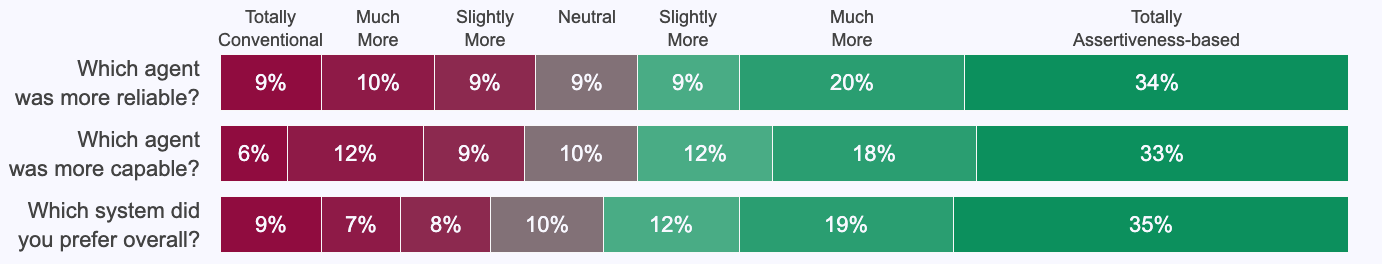
\includegraphics[width=1.000\textwidth]{fig085}
\caption[]{Preference choices of clinicians when comparing both conventional and assertiveness-based agents within this study. Rates of clinicians are ranging from {\it Totally Conventional} to {\it Totally Assertiveness-based} on perceived {\it reliability}, {\it capability}, and {\it overall preference} of each agent.}
\label{fig:fig085}
\end{figure}
%%%%%%%%%%%%%%%%%%%%%%%%%%%%%%%%%%%%%%%%%%%%%%%%%%%

Clinicians' perceptions of trust, understanding, competence, and thoughtfulness towards the conventional and assertiveness-based agents were examined (Table~\ref{tab:tab013} on Section~\ref{sec:app005007002}).
The results indicated comparable trustworthiness (F = 19.47, p = 0.06 $>$ 0.05) between the agents.
No significant differences (p = 0.14 $>$ 0.05) in understanding were found.
The assertiveness-based agent was perceived as more competent (p = 0.04 $<$ 0.05), and clinicians showed higher thoughtfulness with this agent (p = 0.001 $<$ 0.05).
These findings partially support our hypothesis ({\bf H2.2.}) on preference choices.

We assessed the workload and usability of the conventional and assertiveness-based agents and found no significant differences.
There were no significant differences in the workload scores measured by the \ac{NASA-TLX} (p = 0.38 $>$ 0.05) and no significant differences in the usability scores measured by the \ac{SUS} (p = 0.38 $>$ 0.05).
These results support our hypothesis ({\bf H2.3.}) that personalization will not increase clinicians' workload nor decrease usability, with no significant differences between agents.

Last, we examined how clinicians perceive the levels of assertiveness in communicating clinical arguments (Figure~\ref{fig:fig091} on Section~\ref{sec:app005007002} of Appendix~\ref{chap:app005}).
The results revealed significant differences in reliability (F = 31.36, p = 0.0001 $<$ 0.05) and capability (F = 18.17, p = 0.0003 $<$ 0.05) between novice and expert clinicians.
These findings support our hypothesis ({\bf H2.4.}) that clinicians' preferences vary based on the assertiveness level of the agent, indicating differing perceptions of clinical arguments.

\subsection{Summarized Qualitative Insights}
\label{sec:chap006006003}

This section provides a summarized overview of the qualitative analysis of clinicians' perceptions and experiences with conventional and assertiveness-based agents.
For a more detailed analysis, refer to Section~\ref{sec:app005007003} of Appendix~\ref{chap:app005}.
We used a participatory approach to analyze the data collected from focus group sessions, participant opinions, and transcripts.
Through emergent affinity diagrams, common themes were identified regarding clinicians' perceptions of clinical arguments and visualizations of \ac{AI} recommendations.
This qualitative analysis yielded valuable insights into the impact of assertiveness-based agents on clinicians' workflows and mental models.

The qualitative findings revealed that clinicians overwhelmingly preferred human-interpretable arguments over numeric representations of \ac{AI} output classifications (Section~\ref{sec:app005007003001} of Appendix~\ref{chap:app005}).
In fact, 92\% of clinicians preferred the personalized communication and clinical arguments provided by the assertiveness-based agent over the conventional agent.
They found that the assertiveness-based agent enhanced their decision-making process by providing more meaningful and understandable explanations for the \ac{AI} recommendations.
One junior clinician stated, ``{\it The assertiveness-based gave me a better understanding of the AI's reasoning, which helped me make more informed decisions}'' (C6).

Our qualitative insights provided evidence of how clinicians develop mental models of \ac{AI} agents based on their preconceived notions and comparative experiences (Section~\ref{sec:app005007003002} of Appendix~\ref{chap:app005}).
A clinician described the difference, saying, ``{\it The first AI [assertiveness-based] was outstanding... but in the second AI [conventional] I was frustrated with the lack of communication in comparison to the first one}'' (C48).
Expert clinicians used the communication tone to anticipate wrong \ac{AI} recommendations, while novice clinicians focused on the learning process and patient comparisons.
These observations highlight the importance of personalized and customized communication to cater to the varying needs and expectations of clinicians.
These findings contribute to the growing understanding of the impact of \ac{AI} communication on clinicians' decision-making processes and highlight the importance of designing \ac{AI} systems with user-centered approaches~\cite{10.1145/3491102.3517789}.
Something that was indicated in Chapter~\ref{chap:chap005}.

\section{Discussion}
\label{sec:chap006007}

In this section, we provide a condensed overview of the in-depth discussion presented in Section~\ref{sec:app005008} of Appendix~\ref{chap:app005}, where we explore the insights derived from our study and offer targeted recommendations for designing and integrating intelligent agents into the field of medical imaging.
We studied how personalized and customized communication of an intelligent agent can aid clinicians in their decision-making during medical imaging diagnosis.
We conducted a within-subject to investigate how clinicians perceive assertiveness-based agents differently.
Our results show that assertiveness-based agents can alter clinicians' workflows by increasing the efficiency of clinicians while maintaining overall efficacy.

Our findings revealed that the classification accuracy was unaffected by assertiveness-based communication.
However, the tone of the explanations had a significant influence on the decision-making behavior of novice and expert clinicians.
This emphasizes the need for compliant agents that provide personalized and tailored explanations.
By addressing this, future developments can focus on enhancing the provision of relevant and customized explanations, ultimately improving the effectiveness of intelligent agents in medical imaging diagnosis.
These insights contribute to healthcare, \ac{HCI}, decision support, and \ac{AI} communication research.

\subsection{Design Implications}
\label{sec:chap006007001}

This section explores valuable design implications for developing innovative \ac{AI} systems in the clinical domain.
It covers various topics such as combining diverse knowledge classifiers (Section~\ref{sec:app005008001001}), enriching training models with additional information (Section~\ref{sec:app005008001002}), and designing intuitive and user-friendly \acp{UI} for effective agent communication (Section~\ref{sec:app005008001003}).
The generalizability and broader applicability of the study to other related fields are also discussed (Section~\ref{sec:app005008001004}).
Further in-depth insights and recommendations can be found in Section~\ref{sec:app005008001} of Appendix~\ref{chap:app005}.

Including lesion details and the relevance of classification is crucial for improving decision-making in breast cancer diagnosis (Section~\ref{sec:app005008001001}).
By aligning the \ac{AI} system with clinicians' mental models and providing personalized guidance and explanations, intelligent agents can enhance clinicians' decision-making.
Future research should focus on training models with mixed information to effectively integrate them into clinical workflows.
These insights and recommendations contribute to developing human-centered and efficient medical \ac{AI} systems, ultimately improving clinical outcomes and patient care.

The study suggests that personalization of agent communication can positively impact clinical workflows and trust.
To achieve this, \ac{DL} models must predict mixed clinical arguments and adapt communication based on clinicians' experience and demographics (Section~\ref{sec:app005008001002}).
This approach can be implemented through fused training or separate models for each variable.
Personalizing agent communication and incorporating patient information improves intelligent agents in medical imaging, benefiting decision-making and patient outcomes.

The focus is on evaluating personalized and customized communication between agents and clinicians with different medical experience levels (Section~\ref{sec:app005008001003}), specifically by adapting the communication tone.
While the results suggest its potential effectiveness, future research should explore other clinicians' demographic characteristics or agent behaviors to enhance decision-making (Section~\ref{sec:app005015}).
Qualitative findings indicate clinicians' willingness to adjust communication based on the \ac{AI}'s confidence, a warranting investigation into the impact of different performance actions on decision-making.
In conclusion, this section expands on personalized communication in medical \ac{AI} and emphasizes its potential benefits, considering clinicians' experience and confidence in improving care outcomes.

While caution is needed when generalizing the study's findings to other medical domains (Section~\ref{sec:app005008001004}), the personalized and customized communication techniques identified can benefit various medical diagnoses, considering shared challenges across specialties.
For instance, lung cancer and skin cancer diagnosis could also benefit from tailored agent communication, matching clinicians' expertise and background, resulting in improved accuracy and patient outcomes.
Moreover, studies supporting personalized medicine in \ac{AI}-based systems for diagnosis and treatment guidance further validate the relevance and potential impact of the recommendations beyond assertiveness-based agents.

\subsection{Limitations}
\label{sec:chap006007002}

This section summarizes the analysis of the study constraints discussed in Section~\ref{sec:app005008002} of Appendix~\ref{chap:app005}.
The study on assertiveness-based agents in breast cancer diagnosis faced challenges due to limited clinician availability and remote study conditions, impacting task control and clinician interactions.
Liability implications in medical settings and evolving legal frameworks present further limitations, requiring research and legal developments.
Future efforts should focus on robust frameworks and guidelines to address risks and establish accountability.
Training personalized \ac{DL} models and exploring different agent features are areas for future exploration.

\section{Conclusion}
\label{sec:chap006008}

In this work, we provide a novel perspective on how to personalize and customize the explanations of intelligent agents to human clinicians.
Our results from an experimental study with 52 clinicians comparing a conventional agent to an assertiveness-based agent suggest that the ability of a system to not only exploring how to adapt the communication tone ({\it i.e.}, more suggestive or more assertive), but also provide granular explanations of patient cases has merits for end users.
From our results, the time performance was satisfactory, where clinicians took less 25\% of the time to diagnose a patient with the assertiveness-based agent in comparison to the conventional agent.
As we observed, the caparison between the conventional agent and the assertiveness-based agent was more effective also with the latter in achieving the proper diagnostic of the patient.
Additionally, our results demonstrate that if explanations are adapted taking into account the medical experience of clinicians, accuracy chance of correctly diagnosing a patient is 91\% higher for novice and 78\% higher for expert clinicians.
Last, clinicians are showing an increase in trust, preferring the assertiveness-based agent by being more reliable and capable, as this agent was revealing to be further understandable, competent and thoughtful.
Our work has implications for the design of \ac{AI} systems not only in the medical domains, but also in fields that are facing similar challenges, demanding a personalization of the human-AI interaction.
% If Printing on DOUBLE SIDED pages, the second page should be white.
% Otherwise, comment the following command:
\cleardoublepage
%
% Chapter 7
% #############################################################################
% This is Chapter 7
% !TEX root = main.tex
% #############################################################################
% Change the Name of the Chapter i the following line
\fancychapter{Discussion}
\clearpage
% The following line allows to ref this chapter
\label{chap:chap007}

In this dissertation, we carry out a thorough investigation of the role and design of intelligent agents in high-stakes domains, specifically for critical healthcare environments.
Our thesis spans three primary investigations.
Chapter~\ref{chap:chap004} examines the receptiveness of clinicians to intelligent agents, employing the \ac{UTAUT} model as a lens to scrutinize the various factors influencing technology adoption within the medical imaging field.
Through a human-centered approach, Chapter~\ref{chap:chap005} deepens this exploration by addressing clinicians' experiences and perceptions when using \ac{AI} assistance in radiology, shedding light on potential design interventions for more effective integration of \ac{AI} tools into their workflows.
Finally, in Chapter~\ref{chap:chap006}, we provide a novel perspective on personalizing and customizing the communication of intelligent agents adapted to the characteristics of human clinicians, illustrating its importance in facilitating decision-making processes.
Through these investigations, we bridge the gap between \ac{HCI} and \ac{AI} in healthcare, while making significant strides towards understanding, as well as enhancing the adoption and utility of \ac{AI} technologies in clinical settings.

This chapter presents a compendium of contributions (Section~\ref{sec:chap007001}) toward the overarching thesis statement (Section~\ref{sec:chap007002}) and provides pertinent design recommendations (Section~\ref{sec:chap007003}) to integrate intelligent agents into medical imaging workflows.
Our findings underscore the necessity of compliant agents providing tailored explanations, informing future enhancements in the field (Section~\ref{sec:chap007004}).
The insights derived from this dissertation significantly contribute to \ac{HCI}, decision support systems, and \ac{AI} communication research for healthcare, providing a robust foundation for subsequent investigations and developments in these areas.

\section{Contributions and Impact}
\label{sec:chap007001}

This dissertation serves as a substantial contribution to the interwoven realms of \ac{HCI} and \ac{AI}.
Specifically, within the context of decision-making in high-stakes domains such as healthcare.
It provides meaningful exploration of the intricate relationship between these fields, offering invaluable insights for researchers and practitioners navigating the dynamic landscape of healthcare technology.
The cornerstone of this thesis rests in the comprehensive exploration of integrating intelligent agents within healthcare settings, delving into the intricate dynamics affecting clinicians' adoption and usage of such advanced technologies.
It elucidates many factors that influence the acceptance of these systems, providing an in-depth understanding that bridges \ac{HCI} and \ac{AI} in the context of medical decision-making.
By harnessing the power of \ac{AI} and grounding it in the principles of \ac{HCI}, we present potential pathways for enhancing decision-making processes where decisions are critical.
This cross-disciplinary exploration not only enhances the theoretical underpinnings of the field, but also opens new avenues for practical applications in the design and development of user-centric \ac{AI} technologies for critical environments.
The investigation spans three distinct contexts, detailed next.

Our first contribution centers on elucidating the processes through which intelligent agents can be seamlessly integrated into medical imaging workflows.
Relying on the \ac{UTAUT} model as a guiding framework (Chapter~\ref{chap:chap004}), we unravel the roles played by critical determinants and various moderator variables in accepting \ac{AI} recommendations.
This rigorous exploration unveils nuanced insights into how these factors influence clinicians' readiness to incorporate \ac{AI} systems into their routine clinical workflow.
Our findings not only enrich the theoretical underpinnings regarding the incorporation of \ac{AI} systems in healthcare, but they also provide pragmatic recommendations for designing and implementing these technologies effectively.
A critical facet of our research underscores trust's role in clinicians' interaction with \ac{AI} systems, considering potential behavioral variations among clinicians of diverse demographics.
Consequently, our research asserts that fostering trust by considering these varied factors and characteristics is a crucial component in the successful design and deployment of \ac{AI} systems within healthcare settings.

The second significant contribution of this dissertation is the employment of a human-centered design approach that seamlessly weaves \ac{AI} systems into the intricate domain of medical imaging diagnosis (Chapter~\ref{chap:chap005}).
Our approach forms design interventions for a robust medical assistant tool, capturing user needs for control and comprehension of \ac{AI} methods, thereby enhancing clinicians' decision-making.
The research provides an in-depth analysis of these interventions, emphasizing the criticality of transparency, explainability, and usability in building trust.
From this exploration, we distill vital design recommendations endorsing task-specific evaluations, concrete evidence delivery, and precision and recall metrics calibration.
These findings underscore \ac{HCI} principles' pivotal role in developing efficient, user-centric \ac{AI} systems for healthcare, thus augmenting the synergy between clinicians and \ac{DL} predictions.

Our third essential contribution focuses on personalized and customized explanations from intelligent agents, enabling improved communication with clinicians in the complex realm of medical imaging diagnosis (Chapter~\ref{chap:chap006}).
We carried out a comprehensive experimental study comparing a conventional and an assertiveness-based agent.
The latter proved significantly more effective in offering detailed explanations and tailoring communication to clinicians' medical experiences.
Clinicians favored the assertiveness-based agent, perceiving it as more reliable and proficient due to its enhanced understandability and competence.
This preference led to significant reductions in diagnosis time, implying improved efficiency.
Moreover, accuracy rates in diagnoses rose for both novice and expert clinicians.
We extend these findings to infer implications for \ac{AI} system design in medical domains and other fields requiring personalized \acp{HAII}, highlighting the broad applicability of this human-centered approach.

To summarize, our work contributes to the intertwined fields of \ac{HCI} and \ac{AI}, particularly, within the healthcare sector.
Our investigations span clinician acceptance of \ac{AI} systems, the role of human-centered design, and the importance of personalized explanations from intelligent agents.
The findings provide insights for improving decision-making in healthcare and pave the way for practical applications in crafting user-centric \ac{AI} technologies across critical sectors, signifying a substantial stride in \ac{HAII}.

\section{Thesis Statement Support}
\label{sec:chap007002}

This section supports the claims made in this dissertation (Section~\ref{sec:chap001003} of Chapter~\ref{chap:chap001}), aiming to significantly improve the efficiency of the diagnostic process for cancer patients through a human-centered design approach.
The first claim aligns with the principles of \ac{HCI} that emphasize reducing waiting times and alleviating the workload of clinicians in medical systems.
In fact, \ac{HCI} principles serve as guiding paradigms that prioritize \ac{UCD} methodologies, ensuring that \ac{AI} systems in medical imaging are seamlessly integrated and intuitive for clinicians.
While considering the power of such methodologies to address clinicians' experiences and perceptions, this thesis strives to create intuitive and seamlessly integrated \ac{AI} systems that enhance the diagnostic process.
The second claim aligns with the \ac{HCI} principles of personalizing and customizing \ac{AI} outcomes, emphasizing the importance of explainability and interpretability to foster trust and support informed decision-making.
\ac{HCI} research has highlighted the importance of designing \ac{AI} systems that provide clear explanations and insights, empowering clinicians to understand and trust the \ac{AI}-generated outcomes.
These \ac{HCI} principles reinforce the transformative potential of a \ac{UCD} approach, supporting the claims to enhance the efficiency of the diagnostic process and improve the overall healthcare experience.
Next, we provide a detailed description for each claim, offering fundamental evidence that supports these claims within the context of this thesis.

\vspace{1.00mm}

\begin{displayquote}
{\bf Claim:}
{\it
Through a human-centered design, the outcome of this dissertation aims to significantly improve the efficiency of the diagnostic process for cancer patients by reducing the waiting time from weeks to days, which is critical given the time-sensitivity of cancer treatments.
Additionally, it can reduce the workload of radiologists by decreasing the number of exams to be analyzed by half.
}
\end{displayquote}

\vspace{1.00mm}

Our meticulous human-centered design approach aims to significantly enhance the efficiency of the diagnostic process for cancer patients.
In Chapter~\ref{chap:chap004}, we investigate the integration of intelligent agents into medical imaging workflows, uncovering crucial factors that influence clinicians' acceptance and adoption of \ac{AI}-based systems in radiology.
Our findings enrich the theoretical foundations and provide practical recommendations for designing and implementing these technologies effectively, thereby improving the diagnostic process for cancer patients.
Chapter~\ref{chap:chap005} further advances our first claim by focusing on the human-centered design of \ac{AI} assistance in medical imaging diagnosis.
From our design interventions, we gain valuable insights that support clinicians' decision-making capabilities and satisfaction.
By prioritizing transparency, explainability, and usability, we strive to reduce waiting times and alleviate the workload of radiologists, enhancing the overall efficiency of the diagnostic process.
Collectively, these achievements underscore the potential of a human-centered design approach to significantly improve the diagnostic process for cancer patients and relieve the burden on radiologists.

\begin{displayquote}
{\bf Claim:}
{\it
Broader adaptation and customization of the \ac{AI} outcomes may augment individual clinicians to higher cancer detection rates, as well as a reduction of cost and risk for the patient.
As appealing concepts, personalizing and customizing the \ac{AI} outcomes for each clinician will promote a better understanding of \ac{AI} predictions and explain why \ac{AI} achieved some results.
}
\end{displayquote}

\vspace{1.00mm}

Chapter~\ref{chap:chap006} serves as a compelling support for our second claim, as it sheds light on the significance of personalizing and customizing intelligent agents' explanations within our human-centered design strategy.
The preference shown by clinicians towards the assertiveness-based agent, with its enhanced understandability and competence, further strengthens our claim for the importance of adapting and customizing \ac{AI} outputs to improve the comprehension of \ac{DL} predictions and explanations (Section~\ref{sec:app005008} of Appendix~\ref{chap:app005}).
These findings provide solid evidence that such an approach has the potential to enhance detection rates, reduce costs, and mitigate risks for patients.
Furthermore, our research implications transcend healthcare, demonstrating the versatility of personalized \ac{HAII} in diverse fields.
This confirms our thesis claim and underscores user personalization's transformative potential across contexts.

\section{Design Recommendations}
\label{sec:chap007003}

Our design recommendations are based on several thorough analyses.
The first analysis focused on accepting and adopting intelligent agents into the clinical workflow (Section~\ref{sec:chap004006002}).
Another vital study was optimizing workflow integration (Section~\ref{sec:chap005007003}).
Finally, we explored the power of adapting \ac{AI} systems to specific clinical characteristics (Section~\ref{sec:chap006007001}).
From these analyses, we derived recommendations for future \ac{AI} development, targeting enhanced clinical alignment and workflow efficiency.

\vspace{2.00mm}

\noindent
{\bf Guidance Control}:
To preserve clinicians' control, the system should offer precise explanations of the reasoning behind each \ac{DL} prediction and statistical confidence.
An \ac{AI} system should be designed with enough flexibility that allows clinicians to adjust or even override the final diagnostic when necessary.

\vspace{2.00mm}

In terms of decision-making control, \ac{AI} systems should be designed in a way that augments human decision-making rather than trying to replace it.
For better acceptance and adoption, clinicians should always have the final decision and be able to override the recommendations of \ac{DL} predictions if necessary.
This approach reinforces clinician agency, fosters trust, and ensures clinicians stay in charge of patient diagnosis.
In essence, the role of the \ac{AI} guidance should be viewed as a `decision-support' tool rather than a `decision-maker' tool, emphasizing the importance of human judgment in critical domains.

\vspace{2.00mm}

\noindent
{\bf Variability and Usability}:
Account for variability in behavioral characteristics of clinicians during decision-making and adapt \ac{AI} techniques accordingly.
Enhance understanding and usability of \ac{AI} systems to improve clinician trust.

In our human-centered design approach across several clinical institutions, we prioritize accounting for clinician variability during decision-making, impacting how they interact with \ac{AI} systems.
We recommend customizing \ac{AI} techniques to accommodate diverse clinician needs by aligning system functionalities and interfaces with their contexts, terminologies, and conventions.
This tailored approach enhances \ac{AI} usability, understanding, and clinician trust.
Not only it improves \ac{AI} effectiveness, and efficiency, but also supports collaborative decision-making among clinicians with different behavioral characteristics.

\vspace{2.00mm}

\noindent
{\bf Explainability and Transparency}:
Incorporate explainability functionalities, such as feature importance and granular visualization of the clinical arguments, to enhance clinicians' interpretation and belief in \ac{AI} recommendations, fostering interpretability and transparency.

\vspace{2.00mm}

To improve collaboration between clinicians and \ac{DL} models, prioritize explainability in system design.
Features like severity importance provide insights into the factors considered significant by the intelligent agent in making diagnostic decisions.
This enhances clinicians' understanding and confidence in \ac{AI} recommendations.
Additionally, visualizing detailed results can make complex \ac{AI} algorithms more interpretable, fostering transparency and deepening clinicians' comprehension of \ac{AI} suggestions.
Interactive functionalities should be integrated, allowing clinicians to explore variables and conditions and their impact on \ac{DL} predictions.

\vspace{2.00mm}

\noindent
{\bf Workflow Integration and Optimization}:
Integrate \ac{AI} systems seamlessly into the clinical workflow, optimizing the compatibility, performance, and efficiency of each institution.

\vspace{2.00mm}

\ac{AI} systems should be designed to comprehend and accommodate the unique procedures, guidelines, and standards inherent to each clinical setting.
This can be achieved by mapping the workflow and identifying clinicians' needs for specific tasks.
Additionally, \ac{AI} systems should be designed to adapt and evolve based on user feedback and changing clinical needs, incorporating mechanisms for continuous design improvement.
In this way, the \ac{AI} system can become a valuable tool in the clinical workflow, enhancing productivity and ultimately contributing to diagnostic performance.

\vspace{2.00mm}

\noindent
{\bf Longitudinal Studies and Continuous Evaluation}:
Conduct longitudinal studies and gather feedback to iterate on design-based evolving needs and challenges.

\vspace{2.00mm}

Adopt a longitudinal approach to monitor clinicians' evolving interactions with the \ac{AI} system and to pinpoint emerging challenges and enhancement opportunities.
Collect user feedback through multiple channels like surveys, interviews, and usage data, and iterate on the system's design and functionality based on the insights gathered.
Crucially, include clinical outcomes and efficiency measures in evaluations to ensure the system positively impacts medical workflows.
Be prepared to adapt the \ac{AI} system to significant changes in the clinical landscape, such as new guidelines or technologies.
This commitment to continuous evaluation and adaptation underpins the long-term success of \ac{AI} systems in healthcare.

\noindent
{\bf Combination of Classifiers and Enriched Training Models}:
Implement \ac{AI} systems that align with clinicians' mental models, providing personalized guidance and explanations.
Incorporate mixed information in training models to integrate \ac{AI} systems effectively into clinical workflows.

\vspace{2.00mm}

Design \ac{AI} systems that align with clinicians' mental models by incorporating classifiers that consider multiple factors like patient history, demographic data, and clinical observations.
The classifiers should be trained to consider these varied inputs, providing more holistic and accurate predictions.
To ensure effective integration into clinical workflows, the training of these models should also leverage mixed information.
This could include combining diverse data sources such as clinical notes, laboratory results, and imaging data, enhancing the system's ability to handle complex clinical scenarios.
The system should also explain its recommendations by linking them to relevant data or clinical guidelines, enhancing transparency and trust.
Ultimately, these design approaches can enhance the \ac{AI} system's utility in clinical decision-making and its acceptance by clinicians.

\vspace{2.00mm}

\noindent
{\bf Personalization of Communication}: Develop \ac{DL} models that predict mixed clinical arguments and adapt communication based on clinicians' experience and demographics.

\vspace{2.00mm}

To cater effectively to clinicians' needs, \ac{AI} system development should emphasize personalization.
This involves designing systems to predict mixed clinical arguments by incorporating data such as clinicians' experience level, medical specialty, and demographics.
Experienced clinicians may prefer concise, technical language, whereas less experienced ones might find more straightforward, explanatory language beneficial.
Moreover, tailoring communication to the clinician's specialty ensures the relevance of \ac{AI} recommendations.
This personalization enhances usability and fosters a sense of ownership and trust in the system.
By bridging the gap between technical complexity and clinical applicability, \ac{AI} provides personalized, meaningful insights to augment decision-making.
Additionally, the system should flexibly adjust its communication style based on feedback preferences.

\vspace{2.00mm}

\noindent
{\bf Adapting Communication Tone to Generalizability Concerns}: Adjust the communication tone based on \ac{DL} model confidence and case similarity to address the generalizability concerns effectively.

\vspace{2.00mm}

Ensuring effective communication between clinicians and \ac{AI} systems in the context of \ac{DL} models requires addressing the crucial concern of generalizability.
To achieve this, it is necessary to tailor the communication tone by considering two key factors:
(1) the {\it patients' dissimilarity problem} to the training set; leading to
(2) the {\it potential inaccuracies} in the model's confidence.
To adjust the tone based on confidence levels, it is recommended to incorporate case similarity by evaluating how closely the patient's characteristics align with the training data.
When the model encounters a case that significantly deviates from its training set, it should proactively alert the clinician about potential limitations and encourage further assessment.
Additionally, contextual explanations about the model's training data and its potential impact on predictions can greatly enhance clinicians' interpretability and decision-making abilities.

To conclude, these design recommendations call for \ac{AI} systems in healthcare to augment human decision-making, requiring flexibility and transparency.
Both \ac{HCI} and \ac{AI} communities should collaboratively strive to accommodate the diversity among clinicians and ensure seamless integration of their systems into clinical workflows.
Our recommendations stress continuous evaluation, alignment with clinicians' mental models, and personalization.
Emphasis is also placed on explainability, transparency, and tailored communication to address generalizability concerns.
The ultimate goal is to facilitate effective \ac{AI} integration into clinical institutions, thereby improving medical outcomes and patient care.

\section{Future Work Opportunities}
\label{sec:chap007004}

Our research carves a path for numerous intriguing future explorations.
A compelling next step could involve applying insights from the assertiveness-based agent to other high-stakes domains where pivotal decisions deeply impact individuals' lives, such as airport security or supermarket surveillance.
Additionally, these agents could prove valuable in fields marked by considerable variability in professional expertise.
For example, an assertiveness-based agent could provide \ac{AI} recommendations on optimal publication venues for research scientists.
This would help determine whether our findings hold specific relevance to the medical domain or possess broader applicability across varied professions.

We propose exploring diverse communication tones and enhancing explanation relevance by incorporating lexicon specific to breast modalities.
Unraveling the distinct characteristics of assertive and non-assertive tones, and integrating explanations with precise medical terminology, aims to cultivate a stronger rapport between humans and \ac{AI} systems.
Future work should focus on developing \ac{AI} tools that provide detailed, accurate, and tonally appropriate explanations.
We believe such improvements can enhance breast cancer diagnostic accuracy, leading to more confident and informed clinical decisions.

There is another significant potential for training \ac{DL} models to offer personalized, interpretable arguments, which could strengthen clinicians' trust in \ac{AI} recommendations.
Moreover, studying the impacts of essential functionalities, namely, explanations and tone, under a wider array of conditions is critical (Section~\ref{sec:app005015} of Appendix~\ref{chap:app005}).
For the \ac{AI} community, this means technical adaptations to the \ac{DL} model, while for the \ac{HCI} community, the challenge lies in ensuring transparency and accommodating the behavioral characteristics of the clinicians.

Potential future research directions include investigating clinicians' acceptance of \ac{AI}-based follow-up suggestions and assessing the influence of explanations within \acp{CDSSe}.
Furthermore, executing exploratory thematic analyses of intelligent agents, as well as designing ambiguity-aware \ac{AI} assistants, offers exciting research trajectories.
Advancements in these domains will augment our comprehension of the intersection between \ac{HCI} and \ac{AI} in healthcare, thereby facilitating the creation of enhanced, user-friendly tools for healthcare professionals and promoting improved patient outcomes.
% If Printing on DOUBLE SIDED pages, the second page should be white.
% Otherwise, comment the following command:
\cleardoublepage
%
% Chapter 8
% #############################################################################
% This is Chapter 8
% !TEX root = main.tex
% #############################################################################
% Change the Name of the Chapter i the following line
\fancychapter{Future Work}
\clearpage
% The following line allows to ref this chapter
\label{chap:chap008}

The last chapter (Chapter~\ref{chap:chap007}) discussed the design implications, research limitations, and future directions with a specific focus on the research scope of breast cancer diagnosis.
In this chapter, the document broadly scopes and addresses additional directions for future research in this space of \ac{HAII} collaboration decision-making for complex and explainable functionalities.
As a result, the following sections are detailing the future directions sustained by the work developed under this thesis proposal.

\section{Technology Adoption}
\label{sec:sec008001}

Although the current work under this thesis proposal has already studied the preliminary acceptance and trust of \ac{AI} systems, more work should be done.
To strengthen the thesis evidence for such claims, further work must measure a more detailed technology adoption in the context of medical imaging diagnosis.
In this work, a continuing quest to ensure clinicians' acceptance of \ac{AI} is an ongoing clinical challenge.
However, this challenge has occupied researchers to such an extent that \ac{AI} adoption in the clinical domain is now considered an opportunity.

A substantial level of activity has witnessed the use of a wide range of exploratory techniques, examining many different systems in countless different contexts, to the extent that even the most cursory examination will reveal a variety of user perspectives, contexts, analysis, theories, and research methods~\cite{williams2015unified}.
Such situation has in turn led to an element of confusion, as it is often current to be forced of picking specific characteristics across a wide variety of models and theories.
In response to this confusion, and in order to harmonize the literature associated with acceptance of new systems, Venkatesh et al.~\cite{venkatesh2016unified} developed a unified model~\textendash~created and studied by these authors, the \ac{UTAUT}~\textendash~that brings together alternative views on user and innovation acceptance.

As future work, the thesis proposes the application of a model based on the \ac{UTAUT} constructs to study the determinants for adoption of \ac{AI} systems in medical imaging diagnosis.
The idea is to test the model via confirmatory factor analysis and structural equation modeling while using clinicians' responses (expected n $>$ 300 clinicians) to a formulated \ac{UTAUT} questionnaire.
Future results will show how an increased understanding of a vital role of safety, security, privacy, and trust in usage intention of intelligent agents in these medical fields.
It is expected that such results will show to this thesis how improvements of the workflow performance for a clinical \ac{AI} system is a strong predictor of adoption, while medical professional experience ({\it i.e.}, Interns, Juniors, Middles and Seniors) and medical specialities ({\it e.g.}, Radiologists, Surgeons, Dermatologists, Neurologists, etc) are essential moderators of behavioral intention.
The future empirical findings will provide valuable theoretical contributions to \ac{HCI} and \ac{AI} researchers concerning the design and implementation of intelligent agents by explaining the reasons behind adoption and usage of \ac{AI} systems in the clinical workflow.

The questionnaire will be sent via e-mail to participants and the raw data will be analyzed as follows.
In accordance with the recommendations of the two-stage procedure~\cite{rahi2018investigating}, \ac{CFA} will be used to test validity and reliability of the model~\cite{crede2019questionable}.
\ac{SEM} will be used as a preferable technique to regression as it allows simultaneous analysis of all relationships through multiple regression, while also allowing for both observed and latent variables to be analyzed at the same time, and providing overall fit statistics~\cite{hair2017advanced}.
\ac{CFA} will be conducted in \href{https://www.python.org/}{Python} using \ac{MLE}~\cite{cham2017full}, which will be followed by path analysis of the structural relationships that are also expected to be conducted in \href{https://www.python.org/}{Python} with \ac{SEM} libraries~\cite{igolkina2020semopy}.
Moderation analysis will also be undertaken in \href{https://www.python.org/}{Python}~\cite{hayes2017regression}.

\section{Assertiveness-based Intelligent Agents}
\label{sec:sec008002}

Having mechanisms to obtain and analyse clinicians' behaviour, can help researchers to create a more reliable assistant agent~\cite{Miao2019}.
Concerning medical experience and clinical profile ({\it e.g.}, radiologists, surgeons, etc), the future directions of the thesis will analyse critical behaviour and implement persuasive mechanisms to reduce the rates of \acp{FP} and \acp{FN}.
In particular, personalized persuasion strategies are more effective than non-personalized strategies in reporting the diagnostic or influencing the clinician to take the right decision~\cite{sonntag2016persuasive}.
Thus, it will add great value for researchers in the development of assistant agents for the diagnostic via medical imaging.

In this section, it is presented a proposal for applying {\it BreastScreening-AI} in two scenarios, where clinicians will interact with Assertive and Non-Assertive assistant agents~\cite{pacheco2019alignment, 10.1145/3311350.3347162}.
The assistant will act as a second reader, providing results in terms of improvements on the classification diagnosis ({\it i.e.}, Over-Diagnosis {\it vs} Under-Diagnosis) regarding \acp{FP} and \acp{FN}, as well as efficiency and efficacy in the workflow.
While considerable work is focusing on improving the accuracy of \ac{AI} algorithms, comparatively less work focused on improving the communication between Humans and \ac{AI} to satisfy the clinician's own concerns on the explained (\ac{XAI}) information.
This thesis proposal contributes broadly to new work development by examining what clinicians need when using \ac{AI}-powered image diagnostics with proper communication, the practices they adopt while interacting with these novel communication approaches, and how these communications are affecting the end-user interpretation towards the underlying \ac{AI} algorithms.

To conclude, this section describes a proposal study to understand how the level of assertiveness, displayed by an assistant agent, will impact the clinicians' decision-making process during breast cancer diagnosis.
A proof-of-concept prototype~\textendash~another medical imaging assistant~\textendash~will be developed with two major scenarios of the assistant behaviour:
(1) one scenario for an Assertive assistant; and
(2) a second scenario for a Non-Assertive assistant;
paired with two assistant behaviours:
(i) Proactive; and
(ii) Reactive.

A $4$x$4$ within-subjects experiment (n $>$ 45 clinicians) will be conducted, in which the four Assertive, Non-Assertive, Proactive, and Reactive subjects will be matched with the four categories of radiologists' professional experience, {\it i.e.}, Interns, Juniors, Middles and Seniors.
In a latter study, the rates of \acp{FP} and \acp{FN} will be extracted to understand the patterns of critical behaviour among the four categories of professional experience.
Finally, several strategies are proposed expecting to promote unbiased behaviour per each category of professional experience, improving the \acp{FP} and \acp{FN} rates during diagnostics.

\section{New Explainable Methods}
\label{sec:sec008003}

Explanations for machine decisions and predictions are needed to justify their reliability.
This requires greater interpretability, which often means a need to understand the mechanisms that are underlying the algorithm.
Unfortunately, the ``black-boxe'' nature of \ac{DL} is still unresolved, and many machine decisions are still poorly understood.
Future developments of this thesis must follow literature implementations on explainable (\ac{XAI}) and interpretability methods suggested by research works~\cite{9233366}.
The various methods will show clinicians different dimensions in interpretability research, from provide ``obviously'' explainable and interpretable information in complex patterns of lesions and patient co-variables.
By applying such methods to interpretability in medical imaging, it is hoped that: (1) clinicians can subsequently approach these methods with caution; (2) insights into interpretability will be created with more considerations for the clinical workflow; and (3) initiatives to push forward the generated data and leverage its completeness are encourage.
However, it will be also important to evaluate the quality of explanations and levels of interpretability given by the introduction of these new \ac{XAI} methods.
Therefore, the \ac{SCS}~\cite{andreas2020measuring} will support future studies of this thesis.

\section{Publishing Data}
\label{sec:sec008004}

Image data availability is an important hurdle for implementation of \ac{AI} in the clinical setting.
Both \ac{HCI} and \ac{AI} communities need to be aware of the data source and potential biases, which may affect generalizability of \ac{AI} algorithms.
However, curating and annotating data, as well as computational requirements, are substantial barriers.
Future work will include collecting and curating an overall of data to demonstrate how the information produced by clinicians can be used to train humans and machines.
In this thesis, a dataset will be published including, not only clinical data, but also user results.
On the one hand, the clinical data will be published containing important information to the \ac{ML} algorithms, such as medical images, original classifications and manual segmentations from clinicians.
On the other hand, the user results will be published containing usability (\ac{SUS}) and workload (\ac{NASA-TLX}) measures, as well as trust (\ac{DOTS}) and causability (\ac{SCS}) assessment information, between other future metrics to be applied.
% If Printing on DOUBLE SIDED pages, the second page should be white.
% Otherwise, comment the following command:
\cleardoublepage
%
% -----------------------------------------------------------------------------
% BIBLIOGRAPHY
% Add the Bibliography to the PDF table of contents (not the document table of contents)
\pdfbookmark[0]{bibliography}{bib}
% The bibliography style sheet
% Chose your preferences on the format of the entries and the Labels:
% IEEEtran: Used in general (recommended for IST Thesis)
%           Entries are labelled and sorted by appearance in the document
%           Labels are Numeric inside square brackets
\bibliographystyle{IEEEtran}
%
% Apalike:  Entries formatted alphabetically, last name first, with identation
%           Labels with Autor's Name and Year inside square brackets
%\bibliographystyle{apalike}
%
% Alpha:    Entries formatted with Autor's Name and Year, hanging identation
%           Labels with Autor's abbr. Names and Year inside square brackets
%\bibliographystyle{alpha}
%
% Acm:     Entries formatted with Autor's Name (small Caps), hanging identation
%          Labels are Numeric inside square brackets
%\bibliographystyle{acm}
% The following command resets the 'emphasis' style for bibliography entries
\normalem
% Name of your BiBTeX file
\bibliography{
bibliography/own,
bibliography/references
}
%
% The following command modifies the 'emphasis' style for bibliography entries
\ULforem
% If Printing on DOUBLE SIDED pages, the second page should be white.
% Otherwise, comment the following command:
\cleardoublepage
%
% -----------------------------------------------------------------------------
% HERE GO THE APPENDIXES IF REQUIRED
% If not required just comment the blocks
\appendix
%% First Appendix
\pdfbookmark[1]{Appendix}{appendix}
% #############################################################################
% This is Appendix A
% !TEX root = main.tex
% #############################################################################
\chapter{Appendix}
\label{chap:appendix}

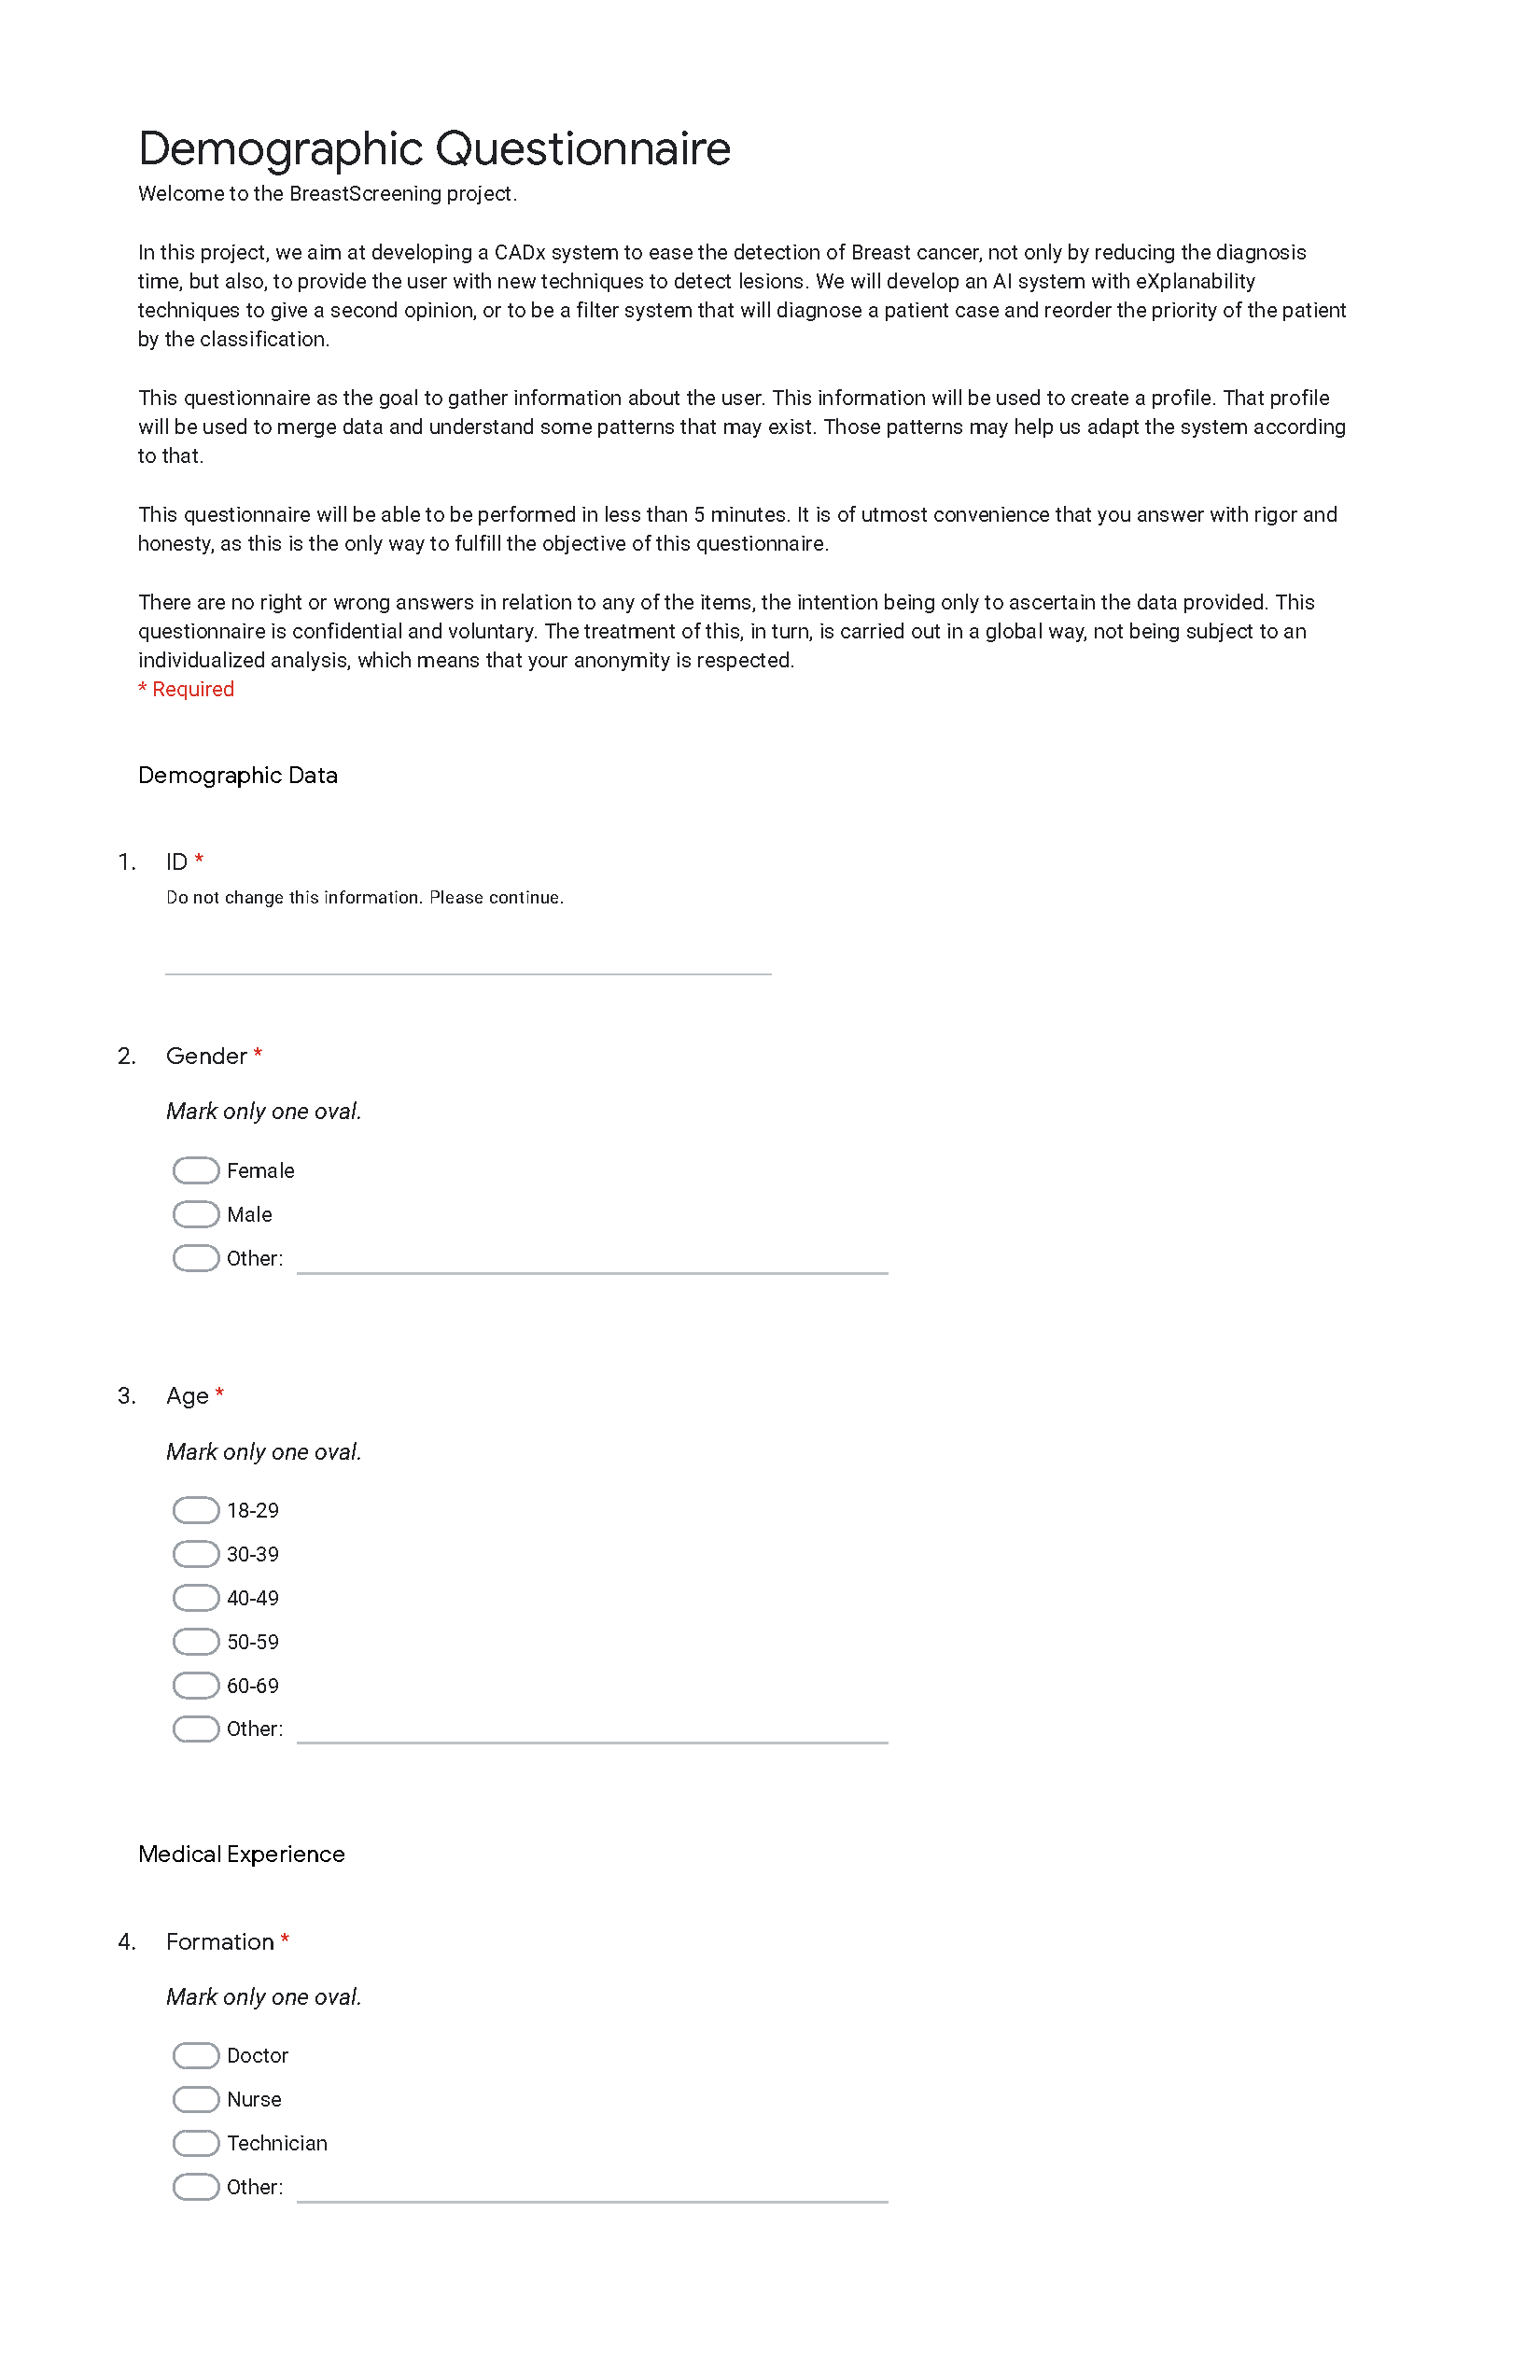
\includepdf[pages=-]{supplements/app001.pdf}
%% If Printing on DOUBLE SIDED pages, the second page should be white.
%% Otherwise, comment the following command:
\cleardoublepage

% -----------------------------------------------------------------------------
% And this is THE END of the IST Thesis Document
\end{document}